%%%%%%%%%%%%%%%%%%%%%%%%%%%%% Define Article %%%%%%%%%%%%%%%%%%%%%%%%%%%%%%%%%%
\documentclass[12pt,a4paper,openany]{My_book}
% \documentclass[12pt,a4paper,openany]{My_article}
% \documentclass[12pt,a4paper]{book}
% \usepackage[pdf]{graphviz}

%%%%%%%%%%%%%%%%%%%%%%%%%%%%%%%%%%%%%%%%%%%%%%%%%%%%%%%%%%%%%%%%%%%%%%%%%%%%%%%

% \usepackage{import} %use of \import functions


%%%%%%%%%%%%%%%%%%%%%%%%%%%%%%%%%%%%%%%%%%%%%%%%%%%%%%%%%%%%%%%%%%%%%%%%%%%%%%%
\newcommand{\size}{0.22\textwidth}
\newcommand{\avg}[1]{\left<#1\right>}
%\newcommand{\condavg}[1]{\left<#1 | \mathscr{C}_1\right>}
\newcommand{\Exp}[1]{\overline{\overline{#1}}}
\newcommand{\davg}[1]{\left<#1\right>_d}
\newcommand{\cavg}[1]{\left<#1\right>_c}
\newcommand{\kavg}[1]{\left<#1\right>_k}
\newcommand{\Iavg}[1]{\left<#1\right>_I}
\newcommand{\pavg}[1]{n \left<#1\right>}
\newcommand{\pnavg}[1]{\left<#1\right>}
\newcommand{\nstavg}[1]{\overline{#1}^{nst}}
\newcommand{\condavg}[2]{\overline{#1}^{#2}}
\newcommand{\nstrelavg}[1]{\overline{#1}_{nst}^{rel}}
\newcommand{\mavg}[1]{\left<#1\right>_m}
\newcommand{\gavg}[2][\gamma]{\left<#2\right>_{#1}}
\newcommand{\partials}[1]{\partial_{i_1}\partial_{i_2}\ldots\partial{i_{#1}}}
\newcommand{\partialp}[2]{ \prod_{m=#1}^{#2} \partial_{i_m}}
\newcommand{\hatpartialp}[2]{ \prod_{m=#1}^{#2} \hat{\partial}_{j_m}}
\newcommand{\hatpartialpi}[2]{ \prod_{m=#1}^{#2} \hat{\partial}_{i_m}}
\newcommand{\pri}[2]{ \prod_{m=#1}^{#2} r_{i_m}}
\newcommand{\prj}[2]{ \prod_{m=#1}^{#2} r_{j_m}}
\newcommand{\nablab}{\bm{\nabla}}
\newcommand{\nablabh}{\hat{\bm{\nabla}}}
\newcommand{\ddt}{\frac{d}{d t}}
\newcommand{\pddt}{\partial_t}
% \newcommand{\pddt}{\partial t \;}
\newcommand{\tb}[1]{\color{blue}#1\color{black}}
% \renewcommand{\tb}[1]{}

% \renewcommand{\ref}[1]{\autoref{#1}}
\renewcommand{\size}[1]{0.3\textwidth}
\newcommand{\expo}[1]{\frac{(-1)^n}{n!} \partialp{1}{n} \pavg{\int_{\Omega_\alpha} \pri{1}{n}#1 d\Omega}}

%%%%%%%%%%%%%%%%%%%%%%%%%%%%%%% Title & Author %%%%%%%%%%%%%%%%%%%%%%%%%%%%%%%%


\title{General overview model for drops suspensions}
\author{Fintzi Nicolas}



\makenomenclature

\includeonly{
    parts/part2_Nearest_Pairs_Statistics
    % parts/part2_intro,
    % parts/part2_Gouverning_eq,
    % parts/part2_Averaged_eq,
    % parts/part2_Lagrangian,
    % parts/part2_Probabilistic_approaches,
    % parts/part2_Lagrangian_averaged,
    % parts/part2_Hybride,
    % parts/part2_closure,
    % parts/part3_intro,
    % parts/part3_physical_description,
    % parts/part3s1,
    % parts/part3s2,
    % parts/part3_Validation,
    % parts/part4_intro,
    % parts/part4_drag,
    % parts/part4_Reynolds_stress,
    % parts/part4_Particule_stress,
    % parts/part4_Statistical_closure,
    % Appendix/Averaging,
    % Appendix/cinematique,
    % Appendix/Exp,
    % Appendix/Equivalence,
}

\begin{document}

\frontmatter
%================================================================
\makeatletter
\begin{titlepage}

\begin{table}[h!]
\begin{minipage}[h]{0.5\linewidth}
% \includegraphics[width=8cm]{Logos/INSA_Texte.png}
\end{minipage}
\hspace{1cm}
\begin{minipage}[h]{0.5\linewidth}
% {\large \textbf{\textsc{Département Génie Mécanique}}}
\end{minipage}
\end{table}

\vfill

%================================================================
%----------------------------------------------------------------
\begin{center}
{\Large\textbf{PhD Thesis}}\\

\vspace{3em}
% \normalsize \hrule height 0.3ex \vspace{0.2ex} \hrule height 0.1ex
\vspace{10pt}
% \title{Investigation on theoritical and numerical macroscopic models aiming to describe emulsions.}
\title{Statistical modeling of disperse two-phases flows : application to buoyancy driven droplets suspensions.}
{\huge\textbf{\@title}} \\
\vspace{10pt}
% \normalsize \hrule height 0.1ex \vspace{0.2ex} \hrule height 0.3ex


\vspace{2em}
\author{\textsc{Fintzi} Nicolas}
{\LARGE \@author}

\vspace{3em}
{\large\textbf{\@date}}\\
% \includegraphics[width=0.5\textwidth]{image/ValidationTriPerio/lescouleurs2.png}
% {\centering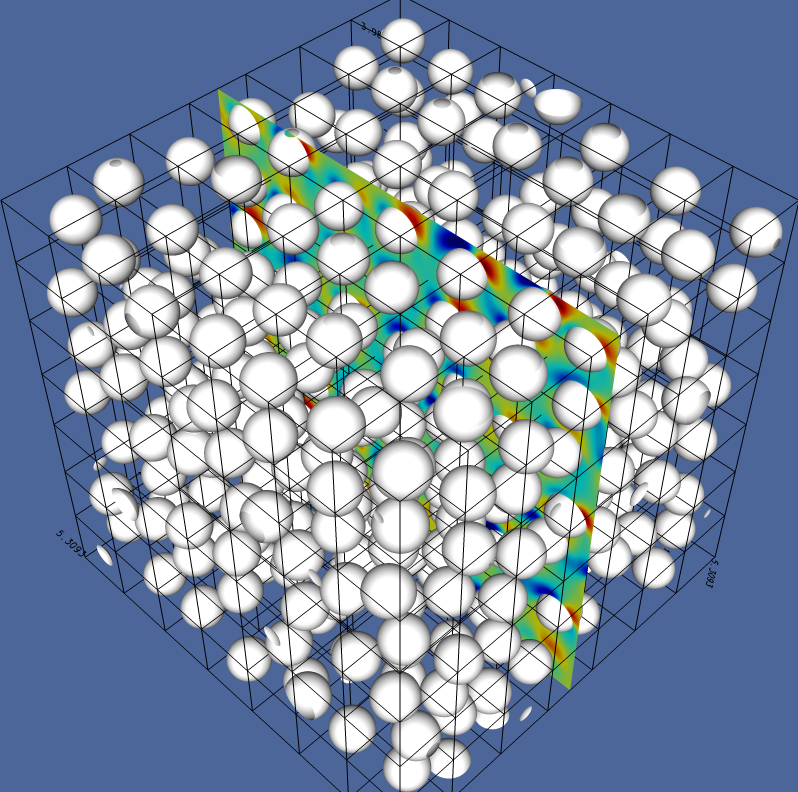
\includegraphics[width = 0.7\textwidth]{image/3D/sim49.png}}
\end{center}
%================================================================


\vfill

%================================================================

\vspace{1em}
\noindent{\large\textbf{Home structure~:} IFPEN Solaize}

\vspace{1em}
\noindent{\large\textbf{Director~:} Stephane \textsc{Popinet}
\footnote[1]{\footnotesize Sorbonne Université, \texttt{21, rue de l'école de médecine, 75006 Paris}. \url{https://www.sorbonne-universite.fr/}}
}

\vspace{1em}
\noindent{\large\textbf{IFPEN supervisors ~:} Jean-Lou \textsc{Pierson}
\footnote[2]{\footnotesize IFP Energies Nouvelles, \texttt{Rond-point de l'échangeur de Solaize, 69360 Solaize}. \url{https://www.ifpenergiesnouvelles.fr/}}
}

%================================================================

\vfill

%================================================================

\includegraphics[height=1.2cm]{image/Logo_IFPEN.png}
\hfill

\includegraphics[height=1.6cm]{image/Sorbonne.jpg}

%================================================================

\end{titlepage}
\makeatother

%================================================================

\hypersetup{linkcolor=black}
\tableofcontents\newpage %\protect\thispagestyle{title}
\listoffigures\newpage
\addcontentsline{toc}{section}{List of figure}
\listoftables
\addcontentsline{toc}{section}{List of tables}

% \section*{Labels}
\nomenclature{$_k$}{Index of the arbitrary  phase $k$}
\nomenclature{$_c$}{Index of the continuous phase $c$}
\nomenclature{$_d$}{Index of the continuous phase $d$}
\nomenclature{$_\alpha$}{Index of the particle $\alpha$}

% \section*{Physical parameters}
\nomenclature{$V_k$}{Volume of the phase $k$  [m$^3$]}
\nomenclature{$\rho_k$}{Density of the phase $k$ [kg.m$^{-3}$]}
\nomenclature{$\mu_k$}{Viscosity of the phase $k$ [kg.m$^{-1}$.s$^{-1}$]}
\nomenclature{$\sigma$}{Surface tension coefficient [N.m$^{-1}$]}
\nomenclature{$g$}{Gravity acceleration [m.s$^{-2}$]}

% \section*{Dimensionless parameters}
\nomenclature{$Ga$}{\textit{Galileo number}}
\nomenclature{$Bo$}{\textit{Bond number}}
\nomenclature{$\mu_r$}{Viscosity ratio}
\nomenclature{$\mu_r$}{Density ratio}
\nomenclature{$N_b$}{Number of droplets}
\nomenclature{$\phi$}{Volume fraction of droplets} 


\nomenclature{$\textbf{x}$}{Macroscopic position vector}
\nomenclature{$\textbf{y}$}{Microscopic position vector}
\nomenclature{$f_k$}{Arbitrary microscopic quantity}
\nomenclature{$\mathbf{\Phi}_k$}{Arbitrary non-convective term}
\nomenclature{$\textbf{S}_k$}{Arbitrary source term}
\nomenclature{$\textbf{u}_k$}{Fluid velocity vector field}
\nomenclature{$\chi_k$}{Phase indicator function}
\nomenclature{$\textbf{n}_k$}{Unit outward normal vector}
\nomenclature{$\delta_I$}{Interface indicator function}
\nomenclature{$\textbf{y}_I$}{Interface position}
\nomenclature{$\textbf{I}$}{Unity tensor}
\nomenclature{$\textbf{u}_I$}{Interfacial velocity vector field}
\nomenclature{$\textbf{J}_I$}{Arbitrary jump field}
\nomenclature{$\kappa$}{Curvature of the interface}
\nomenclature{$M_k$}{Mass transfer term}
\nomenclature{$\textbf{T}_k$}{Stress tensor}
\nomenclature{$p_k$}{Pressure field}
\nomenclature{$\textbf{f}_I$}{Surface tension force}
\nomenclature{$\textbf{b}_k$}{Body forces term}
\nomenclature{$E_k$}{Total energy}
\nomenclature{$e_k$}{Internal energy}
\nomenclature{$\textbf{q}_k$}{Energy heat flux}
\nomenclature{$T_k$}{Temperature}
\nomenclature{$D_k$}{Thermal conductivity}
\nomenclature{$D_k$}{Thermal conductivity}
\nomenclature{$a_I$}{Area density}
\nomenclature{$\phi_k$}{Volume fraction of phase $k$}



\nomenclature{$q_\alpha$}{Arbitrary Lagrangian quantity of the particle $\alpha$}
\nomenclature{$\textbf{Q}_\alpha$}{Arbitrary dipole quantity of the particle $\alpha$}
\nomenclature{$\textbf{Q}_\alpha^n$}{Arbitrary dipole quantity of order $n$}
\nomenclature{$n$}{Number density of particles}
\nomenclature{$A_\alpha$}{Surface of the particle $\alpha$}
\nomenclature{$V_\alpha$}{Volume of the particle $\alpha$}
\nomenclature{$m_\alpha$}{Mass of the particle $\alpha$}
\nomenclature{$\textbf{p}_\alpha$}{Momentum of the particle $\alpha$}
\nomenclature{$\textbf{u}_\alpha$}{Velocity of the particle $\alpha$}
\nomenclature{$\textbf{y}_\alpha$}{Position of the particle $\alpha$}
\nomenclature{$\textbf{w}_k$}{Internal relative velocity of the particle $\alpha$}
\nomenclature{$\textbf{r}$}{Relative position vector}
\nomenclature{$E_\alpha$}{Total energy of the particle $\alpha$}
\nomenclature{$E^\sigma_\alpha$}{Surface energy of the particle $\alpha$}
\nomenclature{$\mathcal{G}_\alpha$}{Inertia tensor}
\nomenclature{$\mathcal{P}_\alpha$}{Moment of momentum tensor}
\nomenclature{$\mathcal{A}_\alpha$}{Angular momentum tensor}
\nomenclature{$\mathcal{S}_\alpha$}{Strain of momentum tensor}

\nomenclature{$\mathscr{C}_N$}{Configuration vector of $N$ particles}
\nomenclature{$P_N$}{Probability density function of $\mathscr{C}_N$ }
\nomenclature{$\Psi$}{Source term related to collision, coalesce and break-up}
\nomenclature{$\theta_\gamma$}{$\gamma^{th}$ Moments of the distribution of $P$}

\nomenclature{$\delta_\alpha$}{Particle indicator function}


% \section*{Mathematical operators}
\nomenclature{$\ddt$}{Time derivative}
\nomenclature{$\pddt$}{Partial time derivative}
% \nomenclature{$\grad$}{Local gradient operator}
\nomenclature{$\gradI$}{Local interfacial gradient operator}
% \nomenclature{$\grad$}{Global gradient operator}
% \nomenclature{$\grad\cdot$}{Local divergence operator}
% \nomenclature{$\grad_I\cdot$}{Local interfacial divergence operator}
% \nomenclature{$\grad_\mathscr{C}\cdot$}{Divergence operator of the phase space}
% \nomenclature{$\grad\cdot$}{Global divergence operator}
\nomenclature{$\avg{\ldots}$}{Ensemble or volume average operator}
\nomenclature{$\kavg{\ldots}$}{Phase average operator}
\nomenclature{$\pnavg{\ldots}$}{Particular average operator}
\nomenclature{$\Iavg{\ldots}$}{Interfacial average operator}
\nomenclature{$\gavg{\ldots}$}{Moment weighted average operator}
\nomenclature{$\mavg{\ldots}$}{Mass weighted average operator}
\nomenclature{$(\ldots)^S$}{Return the symmetric part of the argument}
\nomenclature{$(\ldots)^A$}{Return the antisymmetric part of the argument}
\nomenclature{$\Exp{\ldots}$}{Return the dipole expansion of the argument}

\printnomenclature
\addcontentsline{toc}{section}{Nomenclature}

\newpage

\printacronyms[name=List of acronym]
\addcontentsline{toc}{section}{List of acronym}
\ac{CFD}
\ac{CFD}

% \chapter*{\centering Remerciement}
\phantomsection\addcontentsline{toc}{section}{Acknowledgements}
%\begin{stretchpars}
\noindent 
Je tiens avant tout a remercier Jean-Lou Pierson de m'avoir aceuillie pour mon stage de master à l'IFPEN, puis de m'avoir acceuil une nouvelle fois pour ce sujet de thèse et enfin de m'avoir acceuil une dèrnière fois à l'IFPEN pour un post d'ingénieur ! 
Je te remerci de m'avoir fait découvrir le monde de la recherche, 
de m'avoir enseigner la ``slender-body-theory'' quand je suis arrivé, 
de m'avoir poussé toujours plus loin dans mes projet, 
et de m'avoir fait confiance dans mes idées  (car on a un peu changer le programme de la thèses),
d'être un exemple en terme de rigeurs scientique (ce qui n'était vraiment pas mon fort qd je suis arrivé), 
d'avior toujour sur répondre à mes questions et me guider dans ma thèse vers les bons papiers et livres (merci de m'avoir donné à lire "Jackson 1997" je crois que c'est avec ca que ma thèse a commencé, et de me prêter ta bible: "Jackson 2000", désolé de l'avior un peu abimé d'ailleurs !).
J'ai énormément  appris a travailler à tes cotés, un grand merci !
PS: désolé de t'avoir fait travailler les dimanches sur ma thèse,  maintenant il faut faire de la \textit{slow science} ! 

Merci à Lionel Gamet bien-sur d'avior encadré mon stage de Master 2 également, de m'avoir enseigner les subtiliées de \texttt{Linux} et (particulièrement du fameux \texttt{.rpmmacros}) et de m'avoir appris a faire des maillage butterfly.  
Un plaisir de continuer a travailler avec toi ! 
PS: merci de nous avoir aidés a organiser la soutenance de thèse car on était un peu perdu. 
 
Merci a  Stéphane popinet mon directeur de thèse pour tout ses sage conseilles qui ont su me guider durant toute ma thèse. 
Sache que c'est une fièreté pour moi d'avoir travailler avec toi et d'avoir pu contributer à ton code \texttt{Basilisk}, j'ai bceaucoup appris en matière de programmation quand je me torturais a comprendre comment était codé le \texttt{qcc.h}. 
Merci de m'avior aceuillie a la Sorbonne, et de m'avoir fait présenter mon travail à Daniel Lhuillier et Rodey Fox ce qui constitué le point de départ de ce travail.  
PS: désoloé pour toutes ces fautes d'ortographes quand tu as relu le manuscript ! 

En plus de mes enquadrant j'aimerais bien evidement remercier Daniel Lhuillier qui a pris part à la direction de cette thèse de manière  officieuse. 
Tu m'a montré qu'il était possible d'exposer et de comprendre les equations du modèle hybrid avec simplicitées et pédagogie, ce qui a donner lieu a la rédaction des 3 premier chapitres de ce manuscript, et pour ca je te remercie. 

Je tiens a remercier également les deux rapporteur de cette thèse Duan Zong Zang et Olivier Simonin pour avoir lu ce manuscript en détail et avoir mis en anvant certain problèmes et point important. 
Je remerci égalemnt les autre membre du jury Fabien Candelier, Aurore Naso et Stephane Z. 
Merci a tous les autres chercheur avec qui j'ai pu interagir regulièrement ou ponctuellement cela m'a permis de réaliser ce travail  (Prabuh nott,  Thomas Pathz, Howard Stone.)


Merci à tous les menbres du département R174 pour leurs acceuil quand je suis arrivé en thèse et pour leurs second accueil a mon arrivé en CDI. 
Merci à mes cammarades de thèse Kamel et Paul pour toutes ces discutions scientique inspirantes, et les autres discutions moin scienttifique mais tout autant inspirante; et bon courage a vous pour la suite de la thèse. 

Merci à mes autres amis proche qui se reconnaisseront, et a ma famille pour tout le soutiens porté durant ces trois ans de thèse et plus généralement dans mes étude. 

Enfin merci a Camille Chavassieux qui aura su m'éloigner du travail et m'apporter un soutiens quotidien pour être heureux et équilibré dans la vie.  

\newpage
% \phantomsection\addcontentsline{toc}{chapter}{Front matter}
\chapter*{\centering Abstract}
\phantomsection\addcontentsline{toc}{section}{Abstract}

Buoyancy-driven droplet flows are encountered in many chemical engineering processes such as gravity separators and liquid-liquid extractors. 
These systems exhibit a wide range of scales, from the size of individual inclusions (as small as a few micrometers) to the size of the reactor (often exceeding one meter), making fully resolved simulations computationally impractical.
As a result, the current engineering practice relies on averaged equations of motion for both the dispersed and continuous phases.

Regarding the modeling of dispersed two-phase flows, previous studies have primarily focused on suspensions of solid spherical particles. 
However, significantly less work has been devoted to the modeling of emulsions. 
Hence, the primary focus of this PhD work is the derivation of a set of averaged equations capable of describing suspensions of arbitrarily shaped fluid inclusions and complex surface properties. 
The dispersed phase is represented through Lagrangian-averaged conservation laws, while the continuous phase is modeled using Eulerian-averaged conservation laws. 
Consequently, this formalism is referred to as the ``hybrid model''. 

The second aspect of this PhD is the development of closure models to feed the equations of the ``hybrid model''. 
Specifically, we derive closure laws for the momentum and energy-averaged equations in the dilute and Stokes flow regimes considering mono-disperse emulsions of spherical droplets. 
These theoretical investigations are supplemented by Direct Numerical Simulations (DNS) of buoyant emulsions of droplets, conducted using the open-source code \texttt{Basilisk C}. 
Based on theoretical analysis, DNS results, and findings from the literature, we propose models for the interphase drag force, stresslet tensor, and Reynolds (or pseudoturbulence) stress tensor applicable to rising homogeneous emulsions with finite inertial effects and in non-dilute regimes. 
Our results suggest that including the drift velocity contribution, not only in the inter-phase drag force but also in the effective stress of the continuous phase averaged momentum equation, is essential to model the rheology of emulsions. 

The final contribution of this work concerns the study of the nearest-particle Statistics pair distribution, used to characterize the microstructure of the emulsion and the relative kinematics   of interacting droplets.
It is shown that the microstructure geometry can be described using the second moment of the nearest-particle pair distribution, which quantifies features such as clusters and layers of droplets.
We then analyze the microstructure kinematics through the derivation of a transport equation for this quantity.
In particular, it is shown that the mean interaction time of droplets corresponds to the relaxation time of the second moment of the nearest-particle pair distribution. 
Hence, this timescale governs the formation of the microstructure.


% Overall this PhD work offers mathematical tools necessary to model emulsions within a multiscale ``hybrid'' approach.


\newpage
\chapter*{\centering R\'esum\'e}
\phantomsection\addcontentsline{toc}{section}{R\'esum\'e}

 
Les \'ecoulements de gouttes entra\^in\'es par la flottabilit\'e se rencontrent dans de nombreux proc\'ed\'es de g\'enie chimique, tels que les s\'eparateurs gravitaires et les extracteurs liquide-liquide.
Ces syst\`emes pr\'esentent une large gamme d'\'echelles, allant de la taille des inclusions individuelles (aussi petites que quelques microm\`etres) \`a celle des r\'eacteurs (souvent sup\'erieure \`a un m\`etre), ce qui rend les simulations enti\`erement r\'esolues impossibles \`a r\'ealiser avec les ressources informatiques actuelles.
Par cons\'equent, les pratiques actuelles de mod\'elisation reposent sur l'utilisation des \'equations moyenn\'ees qui d\'ecrive l'\'evolution des phases dispers\'ee et continue.


Concernant la mod\'elisation des \'ecoulements diphasiques dispers\'es, les recherches se sont principalement concentr\'ees sur les suspensions de particules solides sph\'eriques, tandis que beaucoup moins de travaux ont \'et\'e consacr\'es \`a la mod\'elisation des \'emulsions.
L'objectif principal de cette th\`ese est donc la d\'erivation d'un ensemble d'\'equations moyen\-n\'ees capables de d\'ecrire des \'ecoulements dispers\'es avec des inclusions fluides. 
La phase dispers\'ee est repr\'esent\'ee par des lois de conservation lagrangiennes  moyenn\'ees, tandis que la phase continue est mod\'elis\'ee par des lois de conservation eul\'erienne moyenn\'ees.
Ce formalisme est donc appel\'e  ``mod\`ele hybride''.

Le deuxi\`eme aspect de cette th\`ese est le d\'eveloppement de mod\`eles de fermeture pour alimenter les \'equations du  ``mod\`ele hybride'' .
Plus pr\'ecis\'ement, nous d\'erivons des lois de fermeture pour les \'equations moyenn\'ees de quantit\'e de mouvement et d'\'energie cin\'etique dans les r\'egimes dilu\'e et de Stokes, en consid\'erant des \'emulsions monodisperses de gouttes sph\'eriques.
Ces \'etudes th\'eoriques sont compl\'et\'ees par des simulations num\'eriques directes (DNS) d'\'emulsions de gouttes soumises \`a la gravit\'e, r\'ealis\'ees \`a l'aide du code open source \texttt{Basilisk C}.
Avec les analyses th\'eoriques, r\'esultats DNS, et des donn\'ees de la litt\'erature, nous proposons des mod\`eles pour la force de tra\^in\'ee interphasique et le tenseur des contraintes de Reynolds (ou pseudoturbulence), applicables aux \'emulsions homog\`enes ascendantes dans des r\'egimes non dilu\'es et \`a effets inertiels finis.
Nos r\'esultats sugg\`ere que l'inclusion de la contribution de la vitesse relative entre phase dispers\'ee et continue, non seulement dans la force de tra\^in\'ee interphasique, mais aussi dans la contrainte effective de la phase continue, est essentielle pour pr\'edire la rh\'eologie des \'emulsions.

La contribution finale de ce travail concerne l'\'etude de la fonction de corr\'elation de paires des voisines les plus proches, utilis\'ees pour caract\'eriser la microstructure de l'\'emulsion et la cin\'ematique relative des gouttes en interaction.
Nous montrons que la g\'eom\'etrie de la microstructure peut \^etre d\'ecrite en utilisant le second moment de cette distribution, qui quantifie des caract\'eristiques telles que les amas et les couches de gouttes form\'es dans l'\'ecoulement.
Nous proposons ensuite d'analyser la cin\'ematique de la microstructure \`a travers la d\'erivation d'une \'equation de transport pour ce tenseur.
En particulier, il est montr\'e que le temps moyen d'interaction des gouttes correspond au temps de relaxation du second moment de la distribution des paires de particules les plus proches.
Ce temps caract\'eristique gouverne ainsi la formation de la microstructure.

\mainmatter


%chap 1
% \chapter{Introduction}
\label{part:intro}

\tb{Clearly more on floation etc... ask for picture }
\section{Industrial challenges} 
Sedimentation of particles falling or rising under the action of gravity through a fluid is frequently used in a variety of industrial and natural processes, such as food processing, cosmetics, petroleum production, and environmental remediation. 
It is an efficient way to separate solid particles or droplets from the surrounded fluid. 
The clarification of waste water makes use of such a physics, the particles or droplets rise up due to buoyancy forces, afterward they are ejected from the mixture.
Even through numerous experimental and theoretical studies have been conducted on this topic, models are still very restricted and show a significant lack of accuracy. 
In the Perspective of reducing the cost and the environmental impacts of energy processes involving multiphase flows, IFP Energies Nouvelles and public funds, supply finance for the theoretical as well as for experimental research on multiphase flows.
Therefore, this thesis focus on the theoretical and numerical modeling of buoyant emulsion in the context of water waste treatment.  


\section{A multiscale problem} 
The Liquid /Liquid multiphase flows often involve multiscale physical phenomenons. 
Indeed, at the scale of the vessel we can consider the mixture as a homogeneous phase.
The physical properties and the hydrodynamics of the mixture, will depend on the microscale properties and the phases' interactions.
In the context of droplets those interactions are of two kinds. 
The first one is the hydrodynamical interactions between the dispersed phase and continuous phase.
Here, the scale of interest is the droplet scale.
The second type of interaction come from the van der Walls forces which act at the molecular scale. 
Then, we can already identify $3$ scales in this problem.
The scale of the bulk, or the vessel, where the medium seems homogeneous. 
The scale of the droplets, where hydrodynamic forces drive the flow. 
And finally, the molecular scale or the interface scale, where the chemical interaction drive the motions. 
Note that the chemical interactions also involve surfactant which won't be treated in this thesis. 

The link between the vessel's scale and the droplets' scale is usually made using averaged technics. 
It consists in averaging the constitutive equations, that drives the physics at the drop scale, to the reactor scale. 
For isothermal Newtonian flow we generally use the averaged Navier-Stokes equations \citep{jackson1997locally}. 
When we consider specific types of particles or fluid, we need to apply some changes to these equations. 
These averaged equations regardless of the hypothesis taken, involve what we call closure terms.
Those closures are the mathematical expression of the nature of the microstructure.
As an example the averaged drag force on the particles, the velocity fluctuations and the averaged torque and higher moments are closures terms. 
To solve those equations one needs a precise expression of the closure terms. 
Another problem tackled by averaged equations is the modeling of the local size distribution of the droplets. 
The distribution of size can be affected through migration of particles that have different rising velocity as a consequence of their size, and through coalescence and break up of the droplets. 
Note that the particle size distribution is of a major importance as the drag force and the other closure terms depends on it. 
Then, the most challenging part of this problem is not to solve the averaged equations, but rather to find empirical or theoretical closures. 
Regarding the link between the molecular scale and the upper scales, it is done through the modeling of chemical interactions.
Indeed, while the droplets are in contact chemical interaction influence greatly the probability of coalescence and therefore the coalesce rate. 
As a consequence it changes the drops size distribution too.

\section{Non-exhaustive authors cartography of particles suspension dynamics} 
\begin{figure}[h!]
    \begin{tikzpicture}[thick, scale=1, every node/.style={scale=0.5}]
        \node (img) at (0,0){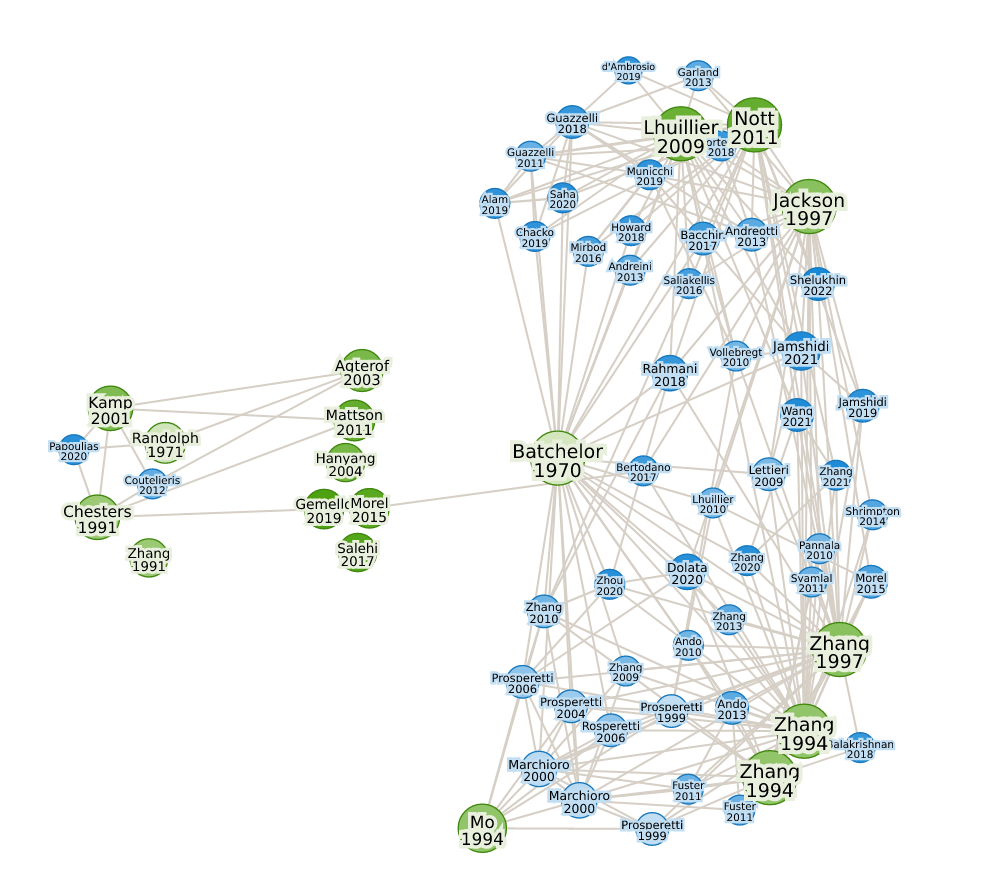
\includegraphics[width=2\textwidth]{Bib/graph70_paperGraph_network.png}};
        \draw[dashed,very thick](-2,-0.5)ellipse(1 and 2.5);
        \draw[dashed,very thick](-5,-0.5)ellipse(1.5 and 2.5);
        \draw[dashed,very thick](4,4)ellipse(2 and 1.5);
        \draw[dashed,very thick](4.5,-4)ellipse(1.5 and 2);
        \draw[dashed,very thick](4,5)node[above,very thick]{\Large$\bm{(III)}$};
        \draw[dashed,very thick](6,-5)node[right,very thick]{\Large$\bm{(II)}$};
        \draw[dashed,very thick](-6.5,2)node[above,very thick]{\Large$\bm{(I)}$};
        \draw[dashed,very thick](-1.3,1.75)node[above,very thick]{\Large$\bm{(IV)}$};
        % \draw[<->](com2.north)--(com3.south)node[midway]{Equivalent};
    \end{tikzpicture}
    \caption{Non-exhaustive cartography of the different publications on population balance models and averaged equations. The articles are represented by the name of the first author. The lines between each article mean that both articles cited each other.}
    \label{fig:carte}
\end{figure}
\ref{fig:carte} summarize the main area related to the theoretical modeling of emulsion through the averaged technics. 
The $\bm{(I)}$ field correspond to the modeling of coalescence and break up phenomenon in a drop or bubbles suspension.
It includes the Population Balance Model (PBM) theory.  
But also the modeling of the film drainage when two drops nearly coalesce. 
Indeed, \citet{randolph2012theory} introduced the first population balance models, at the origin it was designed  for Crystallizes. 
Then, \citet{chesters1991modelling} studied the hydrodynamical and chemical interaction of a pair of droplets leading to coalesce.
And finally, we can observe the first model of PBM including coalescence for a population of droplets \citep{KAMP20011363}.  
The $\bm{(II)}$ and $\bm{(III)}$ area are the authors who studied the averaged equations.
Most of them considered mono-dispersed suspension, therefore the PBE is not involved.
Rather they focused on closing the averaged equations theoretically. 
We consider two district formalism, the one represented here by the main article, \citet{jackson1997locally} and the other by \citet{zhang1994averaged}.
The first one makes use of volume average method and the second one of ensemble average method (those methods will be discussed in \ref{chap:avg}).
To model a poly-disperse suspension of particles (either solid, bubbles or droplet) one has to links the two former theories together, \citep{morel2015mathematical}. 
However, the current state of the art regarding droplets suspension is incomplete.
Therefore, in \ref{chap:avg}, after an entire review of the bibliography, we carry out the derivation of a generalized hybrid model for droplets particles. 
We will see that each of the terms of the averaged equations have a well-defined physical sense related to the nature of the particular phase. 
Then, we address the problematic of the identification of the essential closure terms, and evaluate their relative error while neglecting specific terms. 
Then, in \ref{chap:DNS} we tackle the problematic of the finding of closure terms through Direct Numerical Simulation (DNS).
After identifying the related investigation in the literature, we present our own model and a glimpse of our results in \ref{chap:mono-disperse}. 

\tb{introduce the main equations}

%chap 2
\chapter{The hybrid model for dispersed multiphase flow made of fluid particles}
% \chapterquote{The motion of a suspension can be viewed in two ways.}{R. Jackson}{Poet}
\label{chap:avg}

As stated in \ref{chap:intro} it is computationally too expensive to carry out direct numerical simulation of multiphase flows at the industrial scales. 
Additionally, the microscale interactions themselves are not relevant to optimize these processes, only the macroscopic quantities are significant. 
Therefore, we require laws that can describe the macroscopic scale without having to solve the computationally expensive multiphase problems at the particle scale. 
This is the aim of averaging or Up-scaling technics.
Indeed, by averaging the quantities over a representative volume, timescale or realization, it is possible to derive macro-scale conservation equations for the mean fields, such as the mean velocity and pressure fields. 
Even though we solve these equations for averaged variables, the macro-scale equations still require information related to the microscale phenomena.
The connection between the micro and macro scales is established through different closure laws in these equations. 
These terms, are referred to as the closure terms, they are the mathematical representations of the microscale behavior incorporated into the macro-scale equations
For dispersed multiphase flows, several methods are then available to derive these averaged equations.  
Each of these methods are suited to a given problem depending on the flow's nature and topology. 
In the following, we make an overview of those technics. 

Multiphase flows can be categorized into dispersed flows, such as bubbly flows or emulsions, and arbitrary flows, where the mixture does not exhibit a distinct geometry.
Even though the industrial context of this work focus on dispersed two phases flows we will be interested in a more general formalism in this manuscript. 
Now, let's have a closer look to the different model exposed in the literature. 
Numerous authors introduced theoretical framework to derive averaged equations.
\citet{drew1983mathematical} and \citet{ishii2010thermo} performed ensemble average on the equations of motion, for a mixture of immiscible fluid. 
They make no assumption on the phases' topology therefore this formalism is somewhat the most general. 

Regarding the dispersed two-phase flows, many authors derived averaged equations considering in the first place solely solid spherical particles mono-disperse suspension.
In \citet{jackson1997locally,anderson1967fluid} the continuous-phase conservation equations are averaged with the volume average method.
Then, they consider the dispersed phase as a Lagrangian-phase and perform the average defining an average operator related to the center of mass of the particles instead of their whole volume. 
Consequently, the first set of equations results from the continuous average of the continuous phase equations, and the second from the particular average of the dispersed phase equations, it is therefore known as the \textit{hybrid model}.  
Finally, they considered a suspension of solid spherical particles in the limit of low Reynolds number, and derived theoretical expressions for the closure terms based on classic theoretical results of hydrodynamic.
A different methodology was proposed by \citet{zhang1994averaged} where they also considered a suspension of equal rigid spheres.
They carried out ensemble average method on both phases and derive rigorously the averaged equations similar to \citet{jackson1997locally}.
The closures terms were then derived considering inviscid flows in the dilute limit. 
The statistical averaging method, used in \citet{zhang1994averaged} can  be applied considering an arbitrary number of particles' internal coordinates.  
As an example, in \citet{zhang1994ensemble} they consider variable diameter of spheres with a constant mean diameter and derived with the statistical averaged conservation equations. 
These considerations involve inevitably additional closure terms related to the microscale variation of the diameters.
On another hand, the time averaging method is used by \citet{ishii2010thermo} to derive the macroscopic governing equations, which again, yields the same equations of conservation. 
Although the statistical average turns out to be more practical for the general cases, the other average methods are of course equivalent and lead to the same macroscopic equations. 

Most of the studies mentioned before focus on mono-disperse two phases flows. 
However, fluid-fluid multiphase flows are poly disperse in nature.  
The size distribution of the particles greatly influence the hydrodynamics, energy transfer and mass transfer phenomenons.
Besides, the closure terms of the averaged equations of motion depend highly on the size distribution of particle size. 
Consequently, the population balance equations (PBE) are needed to predict the size distribution in poly disperse flows.
PBE have been derived in the context of Crystallizer in chemical industry \citep{randolph2012theory}.
Numerous authors \citep{marchisio2013computational,fox2022hyperbolic,morel2015mathematical} have been using  and developing those models in the purpose of bubbly flows and emulsion modeling. 

As can be observed, there is numerous framework and tools to average conservation equations for dispersed multiphase flows. 
The suitability of a particular method for the derivation of the averaged equations depend on the physical characteristics of the phases present and the topology of the flow being considered.
In other words, one method may be better adapted than another depending on these factors.
The studies regarding the derivation of the dynamical conservation equations mostly focus on suspension of mono-disperse solid spherical particles.
In some cases they consider other type of particles but still with the mono-disperse assumption.  
As it will be shown the conservation equations using this framework and the PBE use different type of averaging technics and therefore involve different type of averaged velocity fields.
This distinction is often neglected while solving the PBE equations together with the conservation equations from the hybrid models \citet{KAMP20011363}.
While \citep{zaepffel2011modelisation} acknowledges that it is possible to consider the issue, it is noted that doing so can result in mathematical complexities.

In this chapter we present the classic equations of conservation for multiphase flow based on the formulation of \citet{drew1983mathematical,kataoka1986local,ishii2010thermo}. 
Which can be referred to as the \textit{continuous} averaged equations for multiphase flows. 
We then derive a new Lagrangian model for fluid particles, in the continuity of the study of \citet{morel2015mathematical,zaepffel2011modelisation}.
\tb{
By making use of this Lagrangian description, we present the classic way to model poly-dispersity with PBE based on \citet{sporleder2012population,marchisio2013computational,randolph2012theory} and introduce the dynamic Lagrangian equation of kinetic theory.
As it will be shown this formalism is not explicitly linked to the continuous phase averaged equations as both average methods are different.} 
Afterward we apply volume average to the Lagrangian local balance equations, so that we obtain the \textit{particular} averaged equations for the dispersed phase.  
Besides, we demonstrate that it is possible to include change in topology in that model. 
Up to this point we present a set of equation for the continuous phase obtained with the \textit{continuous} averaged method and another for the dispersed phase derived with the \textit{particular} average method. 
Together they form the hybrid model for fluid particles. 
The link and compatibility between the PBE and the classic  generalized hybrid model is discussed, and the latter is shown to fix the inconsistency that the PBE induced. 
On the other hand, as it will be shown in this chapter, the particular averaged equations consider by essence point of mass particles whether it is obtained with statistical approach and PBE or volume averaged Lagrangian equations.
While the continuous average method applied to the dispersed phase by definition doesn't make this point of mass assumption.  
Meaning that two option are available to average the dispersed phase, both leading to different averaged equations as one is continuous and the other discrete. 
Therefore, in the last section of this chapter we address the problem of the equivalence between both method of derivation. 
It is shown that both method are in fact consistent and lead to the same hybrid models but still yields some differences. 
At last, we present the set of equation  and closure terms of the hybrid model for fluid particles.  




\section{Microscopic scale governing equations for two-phase flow}
\label{sec:conservation_laws}

In this section we define the local scale governing equations of multiphase flow using the formulation of \citet{kataoka1986local} and \citet{drew1983mathematical}. 
Before diving into the derivation we would like to emphasize that the local position vector at the local scale is noted $\textbf{y}$.
This clarification will have its usage in the next section where we will use another variable for the global location, namely the vector $\textbf{x}$. 
Also, in this manuscript we write in bold symbols the vectors and tensors, while the scalar variables are written with the usual font. 

Any conservation equation for an arbitrary quantity $f_k(\textbf{y})$, where $f_k$ represent the quantity $f$ but defined in the arbitrary phase $k$, will takes the form,
\begin{equation}
    \pddt f_k
    = \grad \cdot \left(
        \bm{\Phi}_k
        - f_k\textbf{u}_k
        \right)
    + \textbf{S}_k
    \label{eq:general_conservation}
\end{equation}
where $\grad\cdot()$ is the local divergence operator defined as, $\frac{\partial}{\partial \textbf{y}}\cdot()$, $\textbf{u}_k$ is the phase velocity defined in the phase $k$. 
$\bm{\Phi}_k$ is the non-conservative flux corresponding to the quantity $f_k$,
The non-conservative flux is often expressed through a constitutive equation depending on the nature of the flow such as the stress tensor for the momentum. 
And $\textbf{S}_k$ is the volumetric source of $f_k$, such as the body forces still for the momentum equation.
It is important to note that \ref{eq:general_conservation} is solely defined in the volume occupied by the phase $k$.
To generalize the conservation equation over the whole domain, i.e. in each phase and also at the interfaces, we will need supplementary equations. 
To carry out the derivation of these equations we first introduce the Phase Indicator Function (PIF),
\begin{equation}
    \chi_k(\textbf{y}) =  \left\{
      \begin{tabular}{cc}
        $1 \;\text{if} \;\textbf{y} \in V_k$\\
        $0 \;\text{if} \;\textbf{y} \notin V_k$
      \end{tabular}
      \right.,
      \label{eq:phase_indicator}
\end{equation}
with $V_k$ the volume occupied by the $k^{th}$ phase.
As an example, $V_c$ is the volume occupied by the continuous phase and $V_d$ by the dispersed phase. 
With the use of this function we will be able to generalize the phase quantities to general fields, and to derive two kinds of conservation equations, namely, the single-fluid formulation and the two-fluid formulation. 

\subsection{Topological equations}

Before introducing the physical balance equations such as the mass and momentum conservation equations, we study the transport of the volume occupied by a phase $k$ and the interface between the phases considered. 
Therefore, the topological balance equations correspond to the transport equations of $\chi_k$, and the transport of its \textit{roots} along the velocity of its interfaces. 
First, the transport equation of $\chi_k$ reads as \citep{drew1983mathematical,kataoka1986local,morel2015mathematical},
\begin{equation}
    \pddt \chi_k
    + \textbf{u}_I \cdot \grad \chi_k 
    = 0,
    \label{eq:phaseindicator_transport}
\end{equation}
where $\textbf{u}_I$ is the velocity of the interface.
It is important here to make the distinction between the velocity \textbf{of the interface} which is different from the velocity of the phase $k$ \textbf{at the interface} location which is noted $\textbf{u}_k$.
Besides, it can be shown \citep{tryggvason2011direct} that, 
\begin{equation}
    \grad \chi_k 
    = - \delta_I \textbf{n}_k   
\end{equation}
where we have introduced the interface indicator function $\delta_I$, defined as $\delta(\textbf{y}-\textbf{y}_I)$, where $\delta$ is the Dirac-delta function and $\textbf{y}_I$ the position vector of the interfaces. 
We also define $\textbf{n}_k$ as the outward normal vector of the phase $k$. 
We apply the Reynolds transport theorem on $\delta(\textbf{y}-\textbf{y}_I)$, which permit us to obtain the surface balance equation \citep{lhuillier2003dynamics,morel2015mathematical}, 
\begin{equation}
    \pddt \delta_I
    + \grad \cdot\left[
        (\textbf{u}_I\cdot\textbf{n})\textbf{n}\delta_I 
    \right]
    = \delta_I (\textbf{u}_I\cdot\textbf{n})
    (\grad_I\cdot\textbf{n}),
    \label{eq:interface_transport}
\end{equation}
where, $\grad_I$ is the interfacial gradient operator defined as $\grad_I\cdot() = (\textbf{I}-\textbf{nn}):\grad()$.
Note that the normal vector \textbf{n} appear twice in each term, the sign has therefore no importance and there isn't any ambiguity regarding the definition of \textbf{n}, so we removed the index $k$.  
The first term on the right-hand side (RHS) of this equation corresponds to the source term due to the deformation of the interface.
Indeed, it is expressed as the normal velocity $\textbf{u}\cdot\textbf{n}$ times the curvature of the interface defined as $\kappa = - \grad \cdot \textbf{n}$.
Consequently, we can stipulate that the interface evolution is explicitly function of the velocity times the curvature at the interface and its own advection along the interfacial velocity. 
We would like to highlight that this source term doesn't explicitly include topological change in the flow. 
Indeed, it is important to understand that coalescence and break-up phenomenons affect the curvature term, which, in turn, have an impact on the evolution of the interface. 
\footnote{Besides, we will see in the last part of this chapter, that this term is somehow equivalent to the Coalescence kernel of the kinetic theory, which acts directly acts on the area transport equation.} 
As pointed out by \citet{morel2007surface}, this equation can be rewritten under the more common form,
\begin{equation}
    \pddt \delta_I
    + \grad \cdot (\delta_I \textbf{u}_I)
    = \delta_I \grad_I \cdot \textbf{u}_I.
    \label{eq:interface_transport2}
\end{equation}
Note that now the velocity involved is simply $\textbf{u}_I$ and not the normal velocity $\textbf{u} \cdot \textbf{n}$ as in \ref{eq:interface_transport}.
Therefore, this equation has the form of a traditional transport equation, which is the reason why it is preferred. 

\subsection{Generalized balance equations}

As stipulated above, \ref{eq:general_conservation} is solely defined on phase $k$.
We thus need to generalize this equation over the whole domain constituted by all phases.  
There are two possible formulations to carry out this task.
In the following, we give a brief overview of both formulations in the case of a general conservation equation such as \ref{eq:general_conservation}.
The first formulation is the so-called \textit{Two-fluid formulation}.
In this formulation we transport the quantity $f_k\chi_k$, so that $f_k\chi_k$ is defined over the whole domain, since $\chi_k f_k = f_k$ where $\textbf{y} \in V_k$ and $\chi_k f_k = 0$ else where.
So we derive the so called \textit{two-fluid} formulation by multiplying \ref{eq:general_conservation} by the PIF, $\chi_k$ and rearranging each term. 
By making use of the \ref{eq:phaseindicator_transport}, it yields  
\begin{equation}
    \pddt (\chi_k f_k)
    = \grad \cdot (\chi_k \bm{\Phi}_k - \chi_k f_k \textbf{u}_k)
    + \chi_k \textbf{S}_k
    + \left[
        \bm{\Phi}_k 
        + f_k 
        \left(
            \textbf{u}_I
            - \textbf{u}_k
        \right) 
    \right]
    \cdot \textbf{n}_k \delta_I, 
    \label{eq:two-fluid_global}
\end{equation}
where the last term is the interfacial source term representing the interactions across the phases. 
As an example, if $f_k$ turns out to be the momentum, then the interfacial source term would be the drag forces between the phases (see next section). 
For a more detailed derivation of this equation see \ref{ap:average}.
As desired, in this equation all quantities $f_k$ are factor of $\chi_k$. 
So we transport the field $\chi_k f_k$, which is a field quantity defined over the whole domain. 
Note that the interfacial term is factor of $\delta_I$ instead of $\chi_k$ as it is defined on the interface.
Anyhow, \ref{eq:two-fluid_global} is defined over the entire domain and is therefore considered as a valid transport equation. 

The consistency across several phase's conservation equations, is made through the interfacial source term.  
And more precisely it is done with the use of the \textbf{jump condition} at the interface.
It is defined as the sum of the interfacial terms of each phase $k$ over the domain of the interfaces $\textbf{y}_I$. 
It will or will not be null depending on the nature of $f_k$. 
Therefore we define this jump condition as
\begin{equation}
    \sum_k 
    \left[
        \bm{\Phi}_k 
        + f_k 
        \left(
            \textbf{u}_I
            - \textbf{u}_k
        \right) 
    \right]
    \cdot \textbf{n}_k\delta_I
    = \textbf{J}_I\delta_I
    \label{eq:general_jump}
\end{equation}
where $\textbf{J}_I$ is the \textit{jump quantity} related to $f_k$, such as the surface tension force if $f_k$ were the momentum.

Now that we properly defined any conservation laws inside and across each phase, let's derive the \textit{single-fluid} formulation for \ref{eq:general_conservation}.
To do so we sum on all phases \ref{eq:two-fluid_global}, and make use of the jump condition \ref{eq:general_jump} to simplify the interfacial terms. 
Besides, we define the arbitrary quantity $f$ being the sum of the $f_k\chi_k$'s on all phases, i.e. $f = \sum_k \chi_k f_k$.
By taking into account these remarks it is trivial to show that, 
\begin{equation}
    \pddt f
    = \grad \cdot (\bm{\Phi} - f \textbf{u})
    + \textbf{S}
    + \textbf{J}_I \delta_I,
    \label{eq:single-fluid_global}
\end{equation}
which is the \textit{single-fluid} formulation. 
In the following we expose the most important conservation equations for our purpose by replacing $f_k$ or $f$ by the desired quantities.  

\subsection{Mass balances}

Let's introduce the incompressible mass balance for multiphase flows by taking $f_k = \rho_k$. 
According to \ref{eq:two-fluid_global} the \textit{two-fluid} formulation mass balance reads as,
\begin{equation}
    \rho_k\pddt\chi_k
    = 
    - \rho_k\grad\cdot(\textbf{u}_k \chi_k)  
    + \rho_k (\textbf{u}_k-\textbf{u}_I) \cdot \textbf{n}_k \delta_I,
    \label{eq:two-fluid_mass}
\end{equation}
where the first term on the right-hand side (RHS) is the advection of the mass and second term the mass transfer source term.
The points located on the interface must respect the mass jump condition,
\begin{equation}
    \sum_k \left[
        \rho_k (\textbf{u}_k-\textbf{u}_I) \cdot \textbf{n}_k
    \right]
    =\sum_k M_k 
    = 0,
    \label{eq:mass_jump}
\end{equation}
where we introduced the notation $M_k$ to refer to the mass transfer term, and we set $\sum M_k =0$ since any mass leaving a phase is conserved in the neighboring phase.
Note that this equation is valid under the condition that there is no accumulation of mass at the 
interface which is usually what is considered (see \citet{morel2015mathematical}). 

By summing \ref{eq:two-fluid_mass} on all phases and using the jump condition \ref{eq:mass_jump} and the definition of the field quantities we can derive the \textit{single-fluid} formulation of the mass balance equation, namely,  
\begin{equation}
    \pddt \rho
    + \grad\cdot(\rho\textbf{u}_k). 
    = 0 
    \label{eq:single-fluid_mass}
\end{equation}
Note that even though the densities $\rho_k$ are constant in each phase, the overall density $\rho$ isn't since it varies across the phases, therefore it must be considered inside the derivatives.


\subsection{Momentum balances}

We can apply the same routine to obtain the momentum balance equation than for the mass balance, i.e. we transport the momentum field, thus we set $f_k = \rho_k \textbf{u}_k$ in \ref{eq:two-fluid_global}.
Then, the momentum balance in the \textit{two-fluid} formulation is given by,
\begin{equation}
    \pddt (\rho_k \chi_k \textbf{u}_k)
    = \grad \cdot \left(
        \chi_k\textbf{T}_k 
        -\rho_k \chi_k \textbf{u}_k \textbf{u}_k 
    \right) 
    + \textbf{b}_k\chi_k
    +  \delta_I\left(
        M_k \textbf{u}_k
        + \textbf{T}_k \cdot \textbf{n}_k 
    \right),
    \label{eq:two-fuild_momentum}
\end{equation}
where $\textbf{T}_k$ is the stress tensor.
In this work we consider solely Newtonian fluid therefore,
\begin{equation*}
    \textbf{T}_k 
    = -\grad p_k 
    + \mu_k \left[\grad \textbf{u} - (\grad\textbf{u})^T\right],
\end{equation*}
with $p_k$ the pressure field and $\textbf{b}_k$ the body forces present in the phase $k$.
The last term on the RHS is due to the exchange momentum at the interface.
The force acting on the interface is made up of two contribution : the drag force represented by $\textbf{T}\cdot\textbf{n}$, and the momentum transfer resulting from mass exchange, which is represented by $M_k \textbf{u}_k$.
The jump condition at the interface for the momentum reads as, 
\begin{equation*}
    \sum_k \left(
        M_k \textbf{u}_k
        + \textbf{T}_k \cdot \textbf{n}_k
    \right)
    = \textbf{f}_I,
    \label{eq:stressjump}
\end{equation*}
where $\textbf{f}_I$ is the \textit{jump force}. 
If we consider no momentum jump caused by the mass transfer, this force is solely due to the surface tension forces. 
Therefore, it can be expressed as \citep{tryggvason2011direct},  
\begin{equation}
    \textbf{f}_I    
    = \sigma \kappa \textbf{n}
    +\grad_I \sigma,
    \label{eq:f_I}
\end{equation}
where we recall that $\kappa$ is the curvature of the interface defined by $\kappa = -\grad_I\cdot\textbf{n}$ or $\kappa = -\grad\cdot\textbf{n}$. 
We can note that the surface tension force include a term expressed as the divergence of $\sigma$, which is the contribution of non-constant superficial surface tension coefficient which it is commonly known as the  Marangoni forces.
In this work we discard the effect of these forces and consider solely a constant surface tension coefficient.  

Next, we introduce the \textit{single-fluid} formulation of the momentum balance by adding on all phases \ref{eq:two-fuild_momentum} and using the momentum jump condition \ref{eq:stressjump}, 
\begin{equation}
   \pddt (\rho \textbf{u})
    = \grad \cdot (\textbf{T} -\rho  \textbf{u} \textbf{u})
    + \textbf{b}
    + \textbf{f}_I\delta_I.
    \label{eq:one-fuild_momentum}
\end{equation}
where, $\textbf{f}_I\delta_I$ is the contribution of the surface force due to \ref{eq:stressjump} to the bulk momentum $\rho \textbf{u}$. 
It is interesting to note that in the static case, when $\textbf{u}=0$ on all the domain, we recover the famous Laplace equation, i.e. $ -\bm{b} = \hat{\bm{\nabla}}p +\sigma \kappa \textbf{n} $.

\subsection{Energy balance}

Finally, the balance equation for the total Energy transport can be obtained by transporting the total energy $\rho_k E_k$, defined such that $\rho_k E_k = \rho_k(e_k + \frac{1}{2}u_k^2)$, 
where $e_k$ is the internal energy and $u_k^2$ the dot product $\textbf{u}_k\cdot\textbf{u}_k$.
Therefore, $\rho_k E_k$ is the sum of the internal energy and the kinetic energy of phase $k$.
The total energy balance for phase $k$ is obtained by setting $f_k = \rho_k E_k$ in \ref{eq:two-fluid_global} and reads as
\begin{multline}
    \pddt \left(
        \chi_k \rho_k E_k
    \right)
    = \grad \cdot \left[
        \chi_k\left(
            \textbf{T}_k\cdot\textbf{u}_k
            - \textbf{q}_k
            - \textbf{u}_k \rho_k E_k 
        \right)
    \right]
    + \chi_k\textbf{b}_k\cdot\textbf{u}_k\\
    +\left[
        M_k E_k
        + \left(
        \textbf{T}_k\cdot\textbf{u}_k
        - \textbf{q}_k
        \right) 
        \cdot\textbf{n}_k   
    \right]\delta_I,
    \label{eq:two-fuild_totenergy}
\end{multline}
where $\textbf{q}_k$ is the internal energy flux in the phase $k$, usually defined with a Fourier 
law, namely, $\textbf{q}_k = D_k\grad T_k$ with $T_k$ the temperature and $D_k$ the thermal 
conductivity. 
The first term on the RHS correspond to the work of the stress $\textbf{T}_k\cdot \textbf{u}_k$ the internal flux, $\textbf{q}_k$,  and the advection of the total energy, $\textbf{u}_k \rho_k E_k$. 
The source term $\textbf{b}\cdot\textbf{u}_k$ correspond to the work of the body forces. 
Lastly, the interfacial term contains the total energy exchange caused by mass transfer, $M_k E_k$, the exchange of work $\textbf{T}_k\cdot\textbf{u}_k$ due to interfacial stress, and the internal flux from the neighboring phases $\textbf{q}_k$.   
The total energy jump condition reads as, 
\begin{equation}
    \sum_k \left[
        M_k E_k
        + \left(
            \textbf{T}_k \cdot \textbf{u}_k
            - \textbf{q}_k 
        \right)
        \cdot \textbf{n}_k
    \right]
    = \textbf{f}_I\cdot\textbf{u}_I.
    \label{eq:total_energy_jump}
\end{equation}
where we assumed that the \textit{energy jump} is solely due to the work of the interfacial forces. 
Indeed, the jump due to different thermal conductivity and energy mass exchange is not necessarily null. 
However, it will not be addressed in this manuscript as it falls outside the scope of its focus. 

Likewise, the \textit{single-fluid} formulation is given by adding up \ref{eq:two-fuild_totenergy}
on all phases and making use the above jump condition, it is then trivial to show that
\begin{equation}
    \pddt (\rho E)
    = \grad \cdot \left(
        \textbf{T}\cdot\textbf{u}
        - \textbf{q}
        -\rho E \textbf{u} 
    \right)
    + \textbf{b}\cdot\textbf{u}
    +(\textbf{f}_I\cdot\textbf{u})\delta_I.
    \label{eq:one-fuild_totenergy}
\end{equation}
This equation can be split into two distinct equation, one for the kinetic energy and the other for the internal energy. 
The kinetic energy equation is obtained by taking the dot product between 
\ref{eq:two-fuild_momentum} and the velocity vector $\textbf{u}$, yielding,
\begin{equation}
    \frac{1}{2}\pddt (\rho u^2)
    +\frac{1}{2} \grad \cdot (\rho u^2 \textbf{u})
    =\textbf{u}\cdot\left(
        \grad\cdot\textbf{T}
        +\textbf{b}
        +\textbf{f}_I\delta_I.
    \right)
    \label{eq:one-fuild_meca}
\end{equation}
The LHS of this equation is the advection of the kinetic energy $\frac{1}{2}\rho u^2$, while on the RHS we recognize the work of the stress, body forces and surface tension forces. 
Additionally, by taking the difference between the mechanical and the total energy equation, one 
obtain the internal energy equation \citep{tryggvason2011direct}
\begin{equation}
    \pddt (\rho e)
    = 
    \textbf{T}:\grad\textbf{u}
    - \grad\cdot(\textbf{q} + \rho  e\textbf{u}),
    \label{eq:one-fuild_internal_energy}
\end{equation}
where the first term on the RHS is the source term caused by friction in the fluid and the remaining terms have already been defined. 

As a conclusion, in the \textit{two-fluid} approach the interfacial force term is taken into account though the jump condition. 
It is mostly used in theoretical developments, since it describes explicitly the forces between the phases in presence. 
Where in the \textit{single-fluid} method, it is included as a body forces term in the momentum conservation balance (\ref{eq:two-fuild_momentum}) and in the total energy conservation, \ref{eq:two-fuild_totenergy}. 
This formulation allows a greater ease to implement multiphase flows into CFD code for reason that will be detailed in the next section.
More detailed and derivations of these equations can be found in the book of \citet{morel2015mathematical}. 


\section{Averaged equations for two-phase flows.}
\label{sec:introavg}

As stated in the introduction of this chapter we now present the continuous averaged equations for multiphase flow. 
It is important to keep in mind that up to now and all along this section we do not assume anything on the topology of the phase.


\subsection{The averaging concepts}

We start this section by presenting the most common technics of averages and their operators. 
Therefore, we note $\left<f\right>(\textbf{x})$ the average of an arbitrary quantity $f(\textbf{y})$, 
where $\textbf{y}$ is the spacial coordinate in the laboratory reference frame, 
and $\textbf{x}$ macro scale coordinate at which we evaluate the average.
Therefore, we define the \textbf{volume average} operator such as,
\begin{equation}
    \left<f\right>(\textbf{x},t) = \int g(\textbf{x},\textbf{y}) f(\textbf{y},t)dV,
    \label{eq:avg}
\end{equation}
where $g(\textbf{x},\textbf{y})$ is the smoothing (or weighting) function introduced by 
\citet{jackson1997locally,marle1982macroscopic}.
The first argument, $\textbf{x}$, is location at which we take the average, and \textbf{y} is the variable of integration or the local coordinate vector.
The smoothing function $g(\textbf{x},\textbf{y})$ must follow two properties, the first one is normalization to unity 
$\int g(\textbf{x},\textbf{y}) dV = 1 \;\forall g$.
The second one is that $g$ vanish for all $\textbf{y}$ far form $\textbf{x}$, thus $\lim\limits_{|\textbf{r}| \to \infty} g(\textbf{x},\textbf{y}) = 0$ with $\textbf{r} = \textbf{x} - \textbf{y}$.
Also, the radius $R$, of the weighting function $g$, it is defined as $1/2 = \int_{|\textbf{r}|<R} g(\textbf{x},\textbf{y})dV$.
Those characteristics ensure that the integral of \ref{eq:avg} is convergent and well normalized. 

All Eulerian quantities are function of time also. 
Thus, we can average a quantity $f$ on a period of time $T$. 
Therefore, the \textbf{time average} operator is defined such as (see \citet{morel2015mathematical,drew1983mathematical,ishii2010thermo}), 
\begin{equation*}
    \left<f\right>(\textbf{x},t) = \frac{1}{T}\int_{t-T}^t f(\textbf{x},t')dt',
\end{equation*}
with $t$ the time and $t'$ the variable of integration.
Note that the location vector \textbf{x} is the same after and before averaged $f$ since we average over the time dependency of $f$ therefore we use a unique position vector.  

Next, we introduce the ensemble average. 
This averaging technics has been introduced in the context of averaged dispersed 
two-phase flows by \citet{batchelor1972sedimentation,hinch1977averaged} and latter by \citet{zhang1994averaged}.
It is based on statistical approach and defined as follows. 
Let $\mathscr{C}_N$ be a set of parameters describing a configuration of a dispersed two phase flow. 
We then define $P(\mathscr{C}_N,t)$ as the probability density function of being in the configuration $\mathscr{C}_N$ at the time $t$. 
Then for any quantity $f(\mathscr{C}_N,\textbf{x},t)$ of the flow, we can define the \textbf{ensemble average} operator as
\begin{equation}
    \label{eq:enselblea}
    \avg{f}(\textbf{x},t) 
    = \int f(\mathscr{C}_N,\textbf{x},t) P(\mathscr{C}_N)d\mathscr{C}_N,
\end{equation}
where the integration is on all the realization $\mathscr{C}_N$. 
This method is somewhat more general because it allows averaging over an entire 
phase-space of parameters, unlike the two previous methods. 
This averaging technics is widely used in kinetic theory or in turbulence while deriving the Maxwell equation  for example, see \citet[Chapter 7]{rao2008introduction}.  

In short, the first method focus on averaging over the timescale, the second over a volume and the third method over all or a set of configuration of the flow.
While, the latter method and the Volume averaged method seem different in a lot of ways it has been shown that there are strictly equivalent \citet{jackson1997locally,zhang1994ensemble}.
In what follow we apply the volume average method to derive the averaged equation of motion, as we think it is more instinctive.
It is important to note that in any averaging process we must respect the separation of 
scale. 
Consequently, we must respect the mathematical constraints, $D\ll R\ll \mathcal{L}$ with $\mathcal{L}$ the size of the domain, i.e. the scale of the vessel in the industrial context of the process. 
Moreover, it is interesting to mention some mathematical properties shared by all the averaging operators. 
For two arbitrary Eulerian fields $f$ and $h$ we have,
\begin{align}
    &\avg{f+h} = \avg{f}+\avg{h}, 
    &\avg{\avg{f}h} = \avg{f}\avg{h}, \nonumber \\
    &\avg{\frac{\partial f}{\partial t}} 
    = \pddt\avg{f}, 
    &\avg{\frac{\partial f}{\partial x_i}}
    = \frac{\partial}{\partial x_i}\avg{f}. 
    \label{eq:avg_properties}
\end{align}
The two first relations are called the Reynolds' rules, the $3^{th}$ one is the Leibniz' 
rule and the last one, the Gauss' rule \citep{drew1983mathematical}.
Besides, it is important to note that the derivative operator of the last equation change of differentiation variable, from \textbf{y} to \textbf{x}, in the context of volume average.
In the following, we use the notation $\grad$ to represent the global gradient operator, $\frac{\partial}{\partial \textbf{x}}$.
Thus, this last property can be re-written as, $\avg{\grad f}= \grad \avg{f}$ in the volume average context \citep{jackson1997locally}.

Now we introduce the subclass operators, or conditional average operators.
The average of the quantity $f$ considering only the volume of the $k^{th}$ phase, will be defined, such that, 
\begin{equation}
    \phi_k \kavg{f} 
    = \avg{\chi_k f_k},
    \label{eq:avg_k_phase}
\end{equation}
where $\phi_k$ is the volume fraction of the phase $k$ at \textbf{x} and $\kavg{\ldots}$ is the conditional average operator on the phase $k$.
It can be obtained by substituting $f$ by $1$ in \ref{eq:avg_k_phase}, it reads,
\begin{equation*}
    \phi_k  
    = \avg{\chi_k}
\end{equation*}
\tb{We recall here that as all the global average operators are all equivalent, thus we adopt here the general notation $\avg{\ldots}$ to refer to a kind of global average.  }
Additionally, from the previous averaging operators, we can define the mass-weighted average operator by
\begin{equation}
    \avg{\rho} \mavg{f} 
    = \avg{\rho f}
    = \sum_k \phi_k \rho_k\kavg{f}.
\end{equation}

Having established averages operators over the volume of both phases independently, we now define one last conditional averaging operator.
Namely, the surface phase average operator,  
\begin{equation}
    a_I\Iavg{f} 
    = \avg{\delta_I f},
    \label{eq:avg_I_phase}
\end{equation}
where $a_I$ is the interfacial area concentration.  
$a_I$ can be thought of the ratio between the surface of the interfaces over the volume where the interface are included. 
It is defined by, 
\begin{equation}
    a_I
    = \avg{\delta_I}.
\end{equation}

Now, we would like to emphasize that the quantities inside phase average, are implicitly defined inside the $k^{th}$ phase so that it avoid redundancies. 
Therefore, $\kavg{f} = \kavg{f_k}= \avg{f_k\chi_k}$.
At the interface however it is not the case, indeed by definition, at the interface the quantities are defined in both phases.
Thus, we adopt the following convention, when averaging an equation on the volume of phase $k$, $\Iavg{f_k}$ will be the interfacial average of $f_k$, with $f_k$ being the quantity $f$ defined on the phase $k$. 
However, $\Iavg{f}$ without the subscript $_k$, will refer to the interface average of the quantity $f$ defined on the neighboring phase of $k$. 

From the \textit{single-fluid} and \textit{two-fluid} equations exposed previously, one can  note that to obtain an averaged equation on the volume of the $k$ phase two choices are available. 
The first one and more logical choice is to apply the global average on the \textit{two-fluid} formulation equations.
Indeed, half the work is already done since our quantities are already product of $\chi_k$ and the average operators commute with the derivatives.
The other way is to take the conditional average on the volume of the $k$ phase on the \textit{single-fluid} formulation. 
Which implies re-doing some algebra which were already done to get this form of the 
equation.
Anyhow, those two methods are of course strictly equivalent.
In the next few sections we follow the same routine as the previous one and expose the conservation equations in both form but under the averaged form. 


\subsection{The averaged topological equations}

We start by averaging the PIF transport equation, or \ref{eq:phaseindicator_transport}. 
Using the phase average operator \ref{eq:avg_k_phase}, we can easily show that
\begin{equation}
    \pddt \phi_k 
    + \grad \cdot \left(
        \kavg{\textbf{u}}\phi_k 
    \right) 
    = a_I\Iavg{(\textbf{u}_k-\textbf{u}_I) \cdot \textbf{n}_k}, 
\end{equation}
which correspond to the transport equation of the volume fraction $\phi_k$ advected by the mean velocity fields $\kavg{\textbf{u}}$.
The term on the RHS is the interface average of the volume exchange term. 
We will see in the next subsection that this equation is strictly equivalent to the averaged mass balance divided by the density.

Regarding the averaged interfacial transport equation, we can obtain it by averaging \ref{eq:interface_transport}, yielding
\begin{equation}
    \pddt a_I
    + \grad \cdot \left(
        a_I
        \Iavg{\textbf{u}}
    \right)
    = - a_I \Iavg{\kappa \textbf{u}_I \cdot \textbf{n}}
    \label{eq:avg_I_a}
\end{equation}
where this equation correspond to the transport equation of the interfacial concentration $a_I$, along the interfacial averaged velocity field $\Iavg{\textbf{u}}$.

\subsection{Average of an arbitrary conservation equation}

From the \ref{eq:two-fluid_global} and the phase average operator definition (\ref{eq:avg_k_phase}) we can show that the phase averaged conservation equation of an arbitrary quantity $f_k$ reads as, 
\begin{equation}
    \pddt (\phi_k\kavg{f})
    = \grad \cdot \left(
        \phi_k \kavg{\bm{\Phi} - f \textbf{u}}
    \right)
    + \phi_k \kavg{\textbf{S}}
    + a_I \Iavg{
        \bm{\Phi}_k \cdot \textbf{n}_k
        + f_k 
        \left(
            \textbf{u}_I
            - \textbf{u}_k
        \right) \cdot \textbf{n}_k
    },
    \label{eq:avg_k_global}
\end{equation}
where we have used the average operator properties \ref{eq:avg_properties}.
Likewise, the jump condition can be averaged too, using \ref{eq:avg}, yielding,
\begin{equation}
    \sum_k 
    \Iavg{
        \bm{\Phi}_k 
        \cdot \textbf{n}_k
        + f_k 
        \left(
            \textbf{u}_I
            - \textbf{u}_k
        \right) 
        \cdot \textbf{n}_k
    }
    = \Iavg{\textbf{J}_I}.
    \label{eq:avg_general_jump}
\end{equation}
So as the microscopic jump condition this equation maintains the consistency between the different averaged quantity in presence. 
Similarly, the bulk or global averaged conservation equation can be obtained averaging \ref{eq:single-fluid_global} yielding,
\begin{equation*}
    \pddt \avg{f}
    = \grad \cdot \avg{\bm{\Phi} - f \textbf{u}}
    + \avg{\textbf{S}}
    + a_I\avg{\textbf{J}_I}.
    \label{eq:avg_global}
\end{equation*}


\subsection{The averaged mass balance equations}

We first consider the mass conservation. 
By applying the phase average operator (\ref{eq:avg}) to the mass conservation (\ref{eq:two-fluid_mass}) one obtain the mass balance of the $k^{th}$ phases, 
\begin{equation}
    \pddt \phi_k 
    + \grad \cdot \left(
        \kavg{\textbf{u}}\phi_k 
    \right) 
    = \frac{a_I}{\rho_k}\Iavg{M_k},
    \label{eq:avg_k_mass}
\end{equation}
Note that it correspond to the transport equation of the mass fraction of the 
$k^{th}$ phase $\rho_k \phi_k$. 
The source term due to mass transfer can also be expressed though the jump condition, 
\ref{eq:mass_jump} as, $a_I\Iavg{M_k} = - a_I\Iavg{M}$, where we recall that $M$ is the mass transfer term of the neighboring phase such as defined by our notation convention adopted in the previous section. 
We can note that taking the sum of \ref{eq:avg_k_mass} for every phase $k^{th}$ and using the jump condition \ref{eq:mass_jump}, gives us and equation for the bulk density,
\begin{equation}
    \pddt \avg{\rho}
    + \grad \cdot 
        \avg{\rho\textbf{u}} 
    = 0,
    \label{eq:avg_mass}
\end{equation}
which is also the global averaged equation of the \textit{single-fluid} formulation of the mass balance. 
Note that it is possible to uncorrelated $\rho$ and $\textbf{u}$ under the global average operator by using the mass weighted average operator, indeed $\avg{\rho\textbf{u}} = \avg{\rho}\mavg{\textbf{u}}$.
Therefore, the mean density is transported by the mass weighted average velocity. 

\subsection{The averaged momentum balance equations}

The averaged momentum conservation equation on the $k$ phase is obtain by applying 
\ref{eq:avg} on \ref{eq:one-fuild_momentum}. 
It directly gives, 
\begin{equation}
    \pddt (\phi_k\kavg{\rho\textbf{u}}) 
    % + \grad\cdot(\phi_k\kavg{\textbf{uu}})
    = \grad\cdot\left(
        \phi_k \kavg{\textbf{T}
        - \rho\textbf{uu}}
    \right)
    +\phi_k\kavg{\textbf{b}}
    + a_I\Iavg{M_k \textbf{u}_k +\textbf{n}_k\cdot\textbf{T}_k},
\end{equation}
Note that the term including the density, are both average on the volume of the phase $k$.
Thus, the density can be taken out the average such as, $\kavg{\rho \textbf{u}} = \rho_k\kavg{\textbf{u}}$ since $\rho$ is constant in each phase. 
Also, the stress and mass transfer terms inside the interfacial term at the RHS of the equation, are both expressed in their own phase as a consequence of the subscript $_k$.
Usually the drag force term is expressed as the force applied on the interface due to the stress from the neighboring phase. 
Similar thinking goes for the mass transfer term. 
Then to introduce such quantities we make use of the jump condition \ref{eq:stressjump}. 
Applying the preceding remarks on the previous equation yields,
\begin{equation}
    \pddt \left(
        \phi_k\kavg{\rho\textbf{u}}
    \right)
    = \grad\cdot\left(
        \phi_k \kavg{
            \textbf{T}
            -\rho \textbf{uu}}
    \right)
    +\phi_k\kavg{\textbf{b}}
    + a_I\Iavg{
        \textbf{f}_I 
        - M \textbf{u} 
        - \textbf{n}\cdot\textbf{T}
    }.
    \label{eq:avg_k_momentum}
\end{equation}
We recall that by dropping the indices on the interfacial terms $M$, $\textbf{n}$ and $\textbf{T}$ refer to the mass transfer stress tensor defined in the neighboring phase. 
Also, the advantage of \ref{eq:avg_k_momentum} is that we clearly see the action of the surface tension force $\textbf{f}_I$ explicitly.

Applying \ref{eq:avg} on \ref{eq:two-fuild_momentum} gives the bulk average of the momentum equation, namely,
\begin{equation}
    \pddt 
        \avg{\rho\textbf{u}}
    % +  \grad \cdot \left(
    %     \avg{\rho \textbf{u} \textbf{u}}
    % \right)
    = \grad \cdot \avg{
        \textbf{T}
        -  \rho \textbf{u} \textbf{u}} 
    + \avg{\textbf{b}}
    + \Iavg{\textbf{f}_I}.
    \label{eq:avg_momentum}
\end{equation}
In this equation it is interesting to note that the surface jump force appear as a source term. 
On closed surfaces, i.e. droplets or bubbles surface, the resultant of the force $\textbf{f}_I$ cancel out as a result of the divergence theorem \citep{tryggvason2011direct}. 
Nonetheless, the averaged quantity $\Iavg{\textbf{f}_I}$ is not null, despite the fact that we consider solely closed surfaces.
Indeed, it can be shown that this force has the form 
\begin{equation*}
    \avg{\textbf{f}_I}
    = \nabla \cdot \textbf{M}_I + \mathcal{O}(D^2/R^2),
\end{equation*} 
with $\textbf{M}_I$ being a second order tensor that has the form of a stress. 
This point will be discussed in \ref{sec:hybrid_model} were we demonstrate that any averaged quantity can be express as a Taylor expansion series of higher order moments. 

\subsection{The averaged energy balance equations}

Likewise, we apply \ref{eq:avg} to \ref{eq:two-fuild_totenergy} to derive the phase averaged total energy equation.
Also, by making use of the jump condition (\ref{eq:total_energy_jump}), it is trivial to show, 
\begin{multline}
    \pddt \left(
        \phi_k\kavg{\rho E}
    \right)
    % + \rho_k \grad \cdot \left(
    %     \phi_k\kavg{\textbf{u} E} 
    % \right)
    % \\
    = \grad \cdot \left(
        \phi_k\kavg{\textbf{T}\cdot\textbf{u}
        - \textbf{q}
        - \rho E \textbf{u} }
    \right)
    + \phi_k\kavg{\textbf{b}\cdot\textbf{u}} \\
    +a_I \Iavg{
        \textbf{f}_I\cdot\textbf{u}_I
        + \left(
        \textbf{q}
        - \textbf{T}\cdot\textbf{u}
        \right) 
        \cdot\textbf{n}
        -M E}.
    \label{eq:avg_k_total_energy}
\end{multline}
The interfacial on the RHS represent, the heat flux directed inside the phase,
the work of the interfacial force from the external phase, the energy transfer due 
to mass transfer, and the work of the interfacial forces.
The other terms have been described in the previous section. 
Again we can derive an equation for the total energy conservation averaged on the whole bulk. 
From \ref{eq:one-fuild_totenergy}, it yields
\begin{equation}
    \pddt \avg{\rho E}
    = \grad \cdot 
        \avg{\textbf{T}\cdot\textbf{u}
        - \textbf{q}
        - \rho E \textbf{u}}
    + \avg{\textbf{b}\cdot\textbf{u}}
    + \Iavg{\textbf{f}_I\cdot\textbf{u}_I}.
    \label{eq:avg_totenergy}
\end{equation}
Again, as previously it is possible to separate, mechanical and internal energy from this general equation. 
The mechanical energy equation is obtained by averaging \ref{eq:one-fuild_meca}, namely,
\begin{equation}
    \frac{1}{2}\frac{\partial }{\partial t}
            \avg{\rho u^2}
    + \frac{1}{2}\grad \cdot 
            \avg{\rho u^2 \textbf{u}}
    = \grad\cdot\avg{\textbf{u}\cdot \textbf{T}}
    +\avg{\textbf{u}\cdot\textbf{b} - \textbf{T}: \grad\textbf{u}}
    +\Iavg{\textbf{u}\cdot\textbf{f}_I}
\end{equation}
Since we considered the \textit{energy jump} as being solely due to the work of the \textit{force jump}, it must appear entirely in this equation. 
Likewise, the internal averaged energy equation is obtained averaging \ref{eq:one-fuild_internal_energy},
\begin{equation}
    \pddt \avg{\rho e}
    + \grad \cdot \avg{\rho  e\textbf{u}}
    = \avg{\textbf{T}:\grad\textbf{u}}
    + \avg{\grad\cdot\textbf{q}}.
\end{equation}
Again, since the \textit{energy jump} is purely mechanical the surface source term do nor appear in this equation. 
Additional, work on the averaged equations of energy is presented in \ref{ap:average}.

\section{Lagrangian description of a single fluid particle}
\label{sec:Lagrangian_desc}

In the previous sections we derived equations of conservation for Newtonian multiphase flows. 
Then we averaged them in a continuous manner, leading us to a set of averaged conservation equations regardless of the topology of the dispersed phase. 
However, as stated in introduction, the industrial context of this work focuses on dispersed multiphase flows. 
Thus, it is important to take advantage of the dispersed nature of the flow. 
Before, introducing the different averaged models considering dispersed phases, it is important to accurately define the conservation laws acting on a single particle. 
It may seem trivial at first, nevertheless for a whole fluid particle immersed in a Newtonian fluid the Lagrangian balance equations turns out be quite complicated. 

Therefore, in this section we present a complete set of Lagrangian equations describing the evolution of the Lagrangian particle's properties within time. 
We first give a rigorous definition of what is a Lagrangian property for a whole fluid particle. 
Then, we derive general balance equations similar to \ref{eq:general_conservation}, but for a Lagrangian particle. 
Afterward we expose the mass, linear momentum and energy conservation laws.
Additionally, we present a method to describe the evolution of the shape, angular and strain of momentum, and more generally any higher order properties related to a whole fluid particle. 

\subsection{Definition of the Lagrangian properties}

Let us define a particle indexed, $\alpha$, occupying the volume $V_\alpha(t)$ having a Lagrangian property $q_\alpha(t)$.
Then $q_\alpha(t)$ is defined as the mean of the arbitrary Eulerian quantity $f_k(\textbf{y},t)$ over the domain $V_\alpha(t)$, or a subdomain included in $V_\alpha(t)$.
In this section the phase $k$ represent the phase of the dispersed phase as it is arbitrary. 
Therefore, we define $q_\alpha(t)$ such as 
\begin{equation}
    q_\alpha(t)
    = \int_{\Omega_\alpha(t)} f_k(\textbf{y},t) d\Omega,
    \label{eq:q_alpha}
\end{equation}
where $\Omega_\alpha(t)$ is the domain defined such that $\Omega_\alpha \subseteq  V_\alpha$.
Usually, we transport volume quantities, therefore in most of the cases $\Omega_\alpha = V_\alpha$, but it can also be surface quantities, in which case $\Omega_\alpha = S_\alpha$, where $V_\alpha$ and $S_\alpha$ are respectively the volume and surface of the particle $\alpha$.
As an example, $q_\alpha$ is the mass of the particle $\alpha$ when $f_k = \rho_k$ in \ref{eq:q_alpha}.
Also, if $f_k$ has the form of an arbitrary quantity times the surface identification function, i.e. $f_k = f_k \delta_I$, then it is possible to write, 
\begin{equation}
    q_\alpha(t)
    = \int_{V_\alpha} f_k(\textbf{y}) \delta_I dV,
    = \int_{S_\alpha} f_k(\textbf{y}) dS,
    \label{eq:q_surf_alpha}
\end{equation}
in which case $\Omega_\alpha$ turns out to be $S_\alpha$. 
So both expressions remain equivalent. 

All along this section we refer to the Lagrangian quantities labelled by $_\alpha$ solely for quantities that are owned by the particle indexed $\alpha$.
Since, all Lagrangian quantities depend solely on time we discard the argument $t$ in all variables indexed $\alpha$.

\subsection{Generalized balance equations}

For any arbitrary Lagrangian quantity $q_\alpha$ we wish to define its evolution within time. 
To do so, we carry out the total derivative of $q_\alpha$, namely $\ddt q_\alpha$, thanks to Reynolds transport theorem.
So let's introduce the general Reynolds transport equation for any quantity $q_\alpha$, namely, 
\begin{equation*}
    \ddt  q_\alpha 
    = \ddt \int_{V_\alpha} f_k dV 
    = \int_{V_\alpha} \pddt f_kdV 
    + \int_{S_\alpha} f_k \textbf{u}_I \cdot \textbf{n}_k d S,
\end{equation*}
where $\textbf{u}_I$ is the velocity of the interface and $\textbf{n}_k$ the unit outward normal vector to $S_\alpha$. 
By adding and subtracting, $\int_{S_\alpha} f_k \textbf{u}_k\cdot \textbf{n}_k dS$ on the RHS,  this integral can be reformulated as,
\begin{equation}
    \ddt  q_\alpha 
    = \int_{V_\alpha}\left[ \pddt f_k + \grad \cdot\left(f_k\textbf{u}_k\right) \right]dV 
    + \int_{S_\alpha} f_k (\textbf{u}_I-\textbf{u}_k)\cdot \textbf{n}_k d S,
    \label{eq:q_alpha_dt}
\end{equation}
where we clearly distinguish, the volume integral of the local material derivative (first term), and the surface integral of the flux of $f_k$ across the phases (second term).
By substituting the first term with the general conservation law from \ref{eq:general_conservation}, it is straightforward to show that 
\begin{equation}
    \ddt  q_\alpha 
    = \int_{V_\alpha} \textbf{S}_k dV 
    + \int_{S_\alpha} \left[\bm{\Phi}_k + f_k (\textbf{u}_I-\textbf{u}_k) \right] \cdot \textbf{n}_k d S,
\end{equation}
where we used the divergence theorem to transform the non-conservative flux $\bm{\Phi}$ to a surface integral. 
The jump condition \ref{eq:general_jump} can be used to rewrite the previous equation into
\begin{equation}
    \ddt  q_\alpha 
    = \int_{V_\alpha} \textbf{S}_k dV 
    + \int_{S_\alpha} \left[\bm{\Phi} + f (\textbf{u}_I-\textbf{u}) \right] \cdot \textbf{n}_k d S
    + \int_{S_\alpha} \textbf{J}_I dS,
    \label{eq:q_alpha_balance}
\end{equation}
where we recall that \textbf{u} and $\bm{\Phi}$ refer to the velocity and the non-conservative flux of the neighboring phase since we dropped the indices (based on the convention that we adopted in \ref{sec:conservation_laws}). 
Besides, notice that we kept the index $k$ on $\textbf{n}_k$ so that it still refer to the normal outward of the particle $\alpha$. 
Now it is clear that the derivative of any integral quantities over the volume of a particle is the sum of the volumetric source term $\textbf{S}_k$ integrated over the volume, the integral of the jump quantity $\textbf{J}_I$ and integral of the non-convective flux and the flux of $f$ across the surface of the particle. 

Next, let's transport the arbitrary surface quantity $f_k \delta_I$.
In this specific case we must use the general Reynolds transport theorem known as the Leibniz integral rule. 
Indeed, it reads as \citep[Appendix B]{morel2015mathematical}, 
\begin{equation}
    \ddt  q^I_\alpha
    = \int_{S_\alpha} f_k dS 
    = \int_{S_\alpha} \left[
        \pddt f_k 
        +   \grad_I \cdot (\textbf{u}_If_k)
    \right]dS,
    \label{eq:q_alpha_I_dt}
\end{equation}
where this relation is valid for any surface topology. 
Notice that fixing $f=1$ in the above equation gives us an equation of transport for the interfacial area of a particle, which can lead us back to the topological balance \ref{eq:interface_transport}. 
This matter will be discussed in the next few sections. 
Additionally, here is another interesting relation that can be applied to the second term on the RHS of \ref{eq:q_alpha_I_dt} \citep[Appendix B]{tryggvason2011direct}, 
\begin{equation}
    \int_{S_\alpha}  \grad_I  \cdot F dS
    = \int_{C_\alpha} F \cdot \textbf{p} dC
    - \int_{S_\alpha} \kappa F \cdot \textbf{n} dS. 
    \label{eq:surf_div_theorem}
\end{equation}
where $F$ is a tensor of any rank, $C_\alpha$ the boundary of $S_\alpha$, $dC$ is an infinitesimal piece of $C_\alpha$, and \textbf{p} is the vector normal to the line $C_\alpha$ and tangent to the surface $S_\alpha$.
Remark that the first term on the RHS is null for closed surface. 
Notice that in this definition, the direction of \textbf{n} doesn't matter as it appear twice in the expression, indeed a second normal vector \textbf{n} appear inside the definition of the curvature $\kappa$. 

\subsection{Area and surface energy equations}

Let's begin by describing the evolution of the particle surface area within time.
It can be obtained simply by setting $f_k = 1$ in \ref{eq:q_alpha_I_dt}.  
In agreement with \citet{morel2007surface} we obtain,  
\begin{equation*}
    \ddt A_\alpha
    = \ddt \int_{S_\alpha} dS
    = \int_{S_\alpha} \grad_I \cdot \textbf{u}_I dS,
\end{equation*}
where $A_\alpha$ is the surface of the particle $\alpha$. 
Using $F = \textbf{u}_I$ in \ref{eq:surf_div_theorem}, and considering a closed surface, yields the following relation, 
\begin{equation}
    \ddt A_\alpha
    = - \int_{S_\alpha} \kappa \textbf{u}_I \cdot \textbf{n} dS,
    \label{eq:A_dt}
\end{equation}
We can notice on the RHS of \ref{eq:A_dt} that only the normal velocity of the interface appears.
Consequently, the area of a particle surface evolve proportionally to local normal velocity times the local curvature of the interface. 

Likewise, let's consider the derivative of the surface energy of a particle, by substituting $f_k$ by $\sigma$ in \ref{eq:q_alpha_dt} (we recall that $\sigma$ is the surface tension coefficient), resulting in 
\begin{equation*}
    \ddt  E^\sigma_\alpha
    = \int_{S_\alpha} \sigma dS 
    = \int_{S_\alpha} \left[
    \pddt \sigma
    - \kappa \sigma (\textbf{u}_I \cdot \textbf{n})
    \right]dS,
\end{equation*}
where we used the divergence theorem on the last term of the RHS. 
If we consider the expression of the surface force \ref{eq:f_I} with a constant surface tension coefficient $\sigma$ we obtain the following simplified expression,
\begin{equation}
    \ddt  E^\sigma_\alpha
    = \int_{S_\alpha} 
    \textbf{f}_I \cdot \textbf{u}_I
    dS.
    \label{eq:E_sigma_dt}
\end{equation}
\ref{eq:E_sigma_dt} shows that the rate of change of the surface energy is strictly equivalent to the work done by the local surface tension force $\textbf{f}_I$. 
This expression will be useful to clarify the contribution of the surface force in the total energy balance equation. 

\subsection{Mass, momentum and total energy balance equations}

The first set of conservation laws that we can derive rather easily, is  the mass, momentum and total energy balance equations. 
Indeed, substituting $f_k$ with $\rho_k$, $\rho_k \textbf{u}_k$ and $\rho_k E_k$  in \ref{eq:q_alpha_balance}, and making use of the previously defined microscopic balance \ref{eq:two-fluid_mass}, \ref{eq:two-fuild_momentum} and \ref{eq:two-fuild_totenergy}, together with the jump condition of each transport equations, i.e. \ref{eq:mass_jump},\ref{eq:stressjump} and \ref{eq:total_energy_jump} lead us to respectively the mass, momentum and total energy balance equations for a whole fluid particle.
These equations read as,
\begin{align}
    \label{eq:dt_m_alpha}
    \ddt m_\alpha 
    % = \ddt \int_{V_\alpha} \rho_k  dV
    &= \int_{S_\alpha} M_k dS
    = - \int_{S_\alpha} M dS, \\
    \label{eq:dt_p_alpha}
    \ddt \textbf{p}_\alpha 
    % = \ddt \int_{V_\alpha} \rho_k \textbf{u}_k dV
    &= \int_{V_\alpha} \textbf{b}_k dV
    + \int_{S_\alpha} \left(
    \textbf{T}\cdot\textbf{n}_k
    + \textbf{f}_I 
    + M_k \textbf{u}_k
    \right)dS, \\
    \label{eq:dt_e_alpha}
    \ddt E_\alpha 
    % = \ddt \int_{V_\alpha} \rho_k E_k dV
    &= \int_{V_\alpha} \textbf{b}_k \cdot \textbf{u}_k dV 
    + \int_{S_\alpha} \left[
        (\textbf{T}\cdot \textbf{u} 
    - \textbf{q})\cdot\textbf{n}_k 
    + M_k E_k 
    + \textbf{f}_I \cdot \textbf{u}_I 
    \right]dS, 
\end{align}
where $m_\alpha =  \int_{V_\alpha} \rho_k dV$, $\textbf{p}_\alpha= \int_{V_\alpha} \rho_k \textbf{u}_k dV$ and $E_\alpha= \int_{V_\alpha} \rho_kE_k dV$ are respectively the mass, momentum and total energy of the particle $\alpha$. 
We recall that $M_k$ is the mass transfer term, $E_k$ the local total energy, \textbf{T} the stress tensor of the neighboring phase, $\textbf{b}_k$ the body forces of the phase $k$, $\textbf{f}_I$ the surface tension force. 
Notice that thanks to the jump condition of the energy and the momentum equation, we made appear the stress and heat flux of the neighboring phase together with the surface tension force. 
Which is more appropriate when dealing with solid particles as the internal stress $\textbf{T}_k$ and heat flux $\textbf{q}_k$ is not always defined. 
It is possible to reformulate these equations in several ways. 
First, if we consider \ref{eq:f_I}, it can be shown that the integral of $\textbf{f}_I$ over a closed surface is null \citep[Appendix B]{tryggvason2011direct}, therefore this term vanishes.
Additionally, by substituting the term $\textbf{f}_I \cdot \textbf{u}_I$ by \ref{eq:E_sigma_dt} in the energy equation we can make appear the surface tension energy.  

Before diving in further details it is crucial to define some fundamental quantities of the particles $\alpha$. 
First, the position of the center of mass of the particle, $\textbf{y}_\alpha$, is defined as, 
\begin{equation*}
    m_\alpha \textbf{y}_\alpha
    = \int_{V_\alpha} \rho_k \textbf{y}_k dV,
\end{equation*}
Additionally, we define the distance between any points inside $V_\alpha$ and $\textbf{y}_\alpha$ by the vector \textbf{r}, such that, $\textbf{r}(\textbf{y},t) = \textbf{y} - \textbf{y}_\alpha(t)$.
Again, we can notice here, and it will be of major importance in the next derivations, that $\textbf{r}$ is function of space and time. 
Now that the position of the center of mass is stated, we can define the point velocity of a whole fluid particle.
The unique and non-arbitrary definition of the particle's center of mass velocity, is that it is the derivative within time of its position vector $\textbf{y}_\alpha$.
Therefore, by making use of the Reynolds transport theorem (\ref{eq:q_alpha_dt}), and classical rules of derivation, it can be shown that (see \ref{ap:average}),  
\begin{equation}
    \textbf{u}_\alpha
    = \frac{1}{m_\alpha} \left(
        \textbf{p}_\alpha
        +  \int_{S_\alpha} \textbf{r} M_k dS
    \right)
    \label{eq:dt_y_alpha}
\end{equation}
where we introduced the notation of the particle's center of mass velocity, 
\begin{equation*}
    \textbf{u}_\alpha = \ddt \textbf{y}_\alpha,
\end{equation*}
and we made use of the momentum definition \ref{eq:dt_p_alpha}.
Notice that the first component of the RHS of the velocity is the linear momentum divided by the mass of the particle.
The second term is less intuitive, it results from the contribution of the anisotropic mass transfer over the surface of the particle. 
We emphasize that this term is different from the momentum exchange term $\int \textbf{u}_kM_k dS$ (in \ref{eq:dt_p_alpha}) as it does not involve momentum exchange, but rather mass exchanges. 
In \citet{zaepffel2011modelisation}, \citet{paisant2014modelisation} and \citet{morel2015mathematical}, they state that the particle's center of mass velocity is $\textbf{u}_\alpha = \textbf{p}_\alpha / m_\alpha$ even though they are considering mass transfer. 
It is indeed what we would expect in most of the cases, nevertheless this definition turns out to be not adapted in the presence of anisotropic mass transfer as denoted by \ref{eq:dt_y_alpha}. 
To give a better understanding on the physical implication of this contribution we propose the following example :
Let consider the particle of volume $V_\alpha$ be represented by a rocket of volume $V_\alpha$.
Then while the rocket is taking off, a considerable amount of kerosene leaves the volume $V_\alpha$ causing mass transfer from the inside to the outside of the rocket's volume.
Then the center of mass of the rocket, $\textbf{y}_\alpha$, rise up because of two distinct contribution.
The first one is because of newton 3$^{th}$ law which stipulate that any transfer of momentum results in a source of momentum in the opposite direction.
This contribution corresponds to the last term of \ref{eq:dt_p_alpha}, namely, $\int \textbf{u}_kM_k dS$.
The second contribution is due to the loss of kerosene in the rocket, which makes the center of mass slightly move upward in the rocket frame of reference, since the mass balance within the rocket changes.
The rate of change of the center of mass is the second contribution to the total velocity, i.e. the second term of \ref{eq:dt_y_alpha}, namely $\int_{S_\alpha} \textbf{r}M_kdS$.  
Knowing that, it is hard to imagine how such contribution could have any importance in the context of dispersed two-phase flows. 
Besides, it is interesting to notice that regardless of the particle's internal motions, the relevant velocity is $\textbf{u}_\alpha = \textbf{p}_\alpha /m_\alpha,$ if we neglect mass transfer.
Also, we define the \textit{inner velocity} $\textbf{w}_k(\textbf{y},t)$, such that $\textbf{w}_k(\textbf{y},t) = \textbf{u}_k(\textbf{y}) - \textbf{u}_\alpha(t)$. 
Using this definition, and after manipulating \ref{eq:dt_y_alpha} we obtain the following relation for the momentum, 
\begin{equation}
    \textbf{p}_\alpha
    =  m_\alpha \textbf{u}_\alpha
    - \int_{S_\alpha} \textbf{r} M_k dS
    = m_\alpha \textbf{u}_\alpha
    + \int_{V_\alpha} \rho_k \textbf{w}_k dV,
    \label{eq:velocity_definition}
\end{equation}
where the step from the second to the third equality is made possible thanks to a relation derived in the next section, see \ref{eq:M_alpha_dt}. 
Anyhow, as we stated above the integral of the innner velocity is \textbf{rigorously null}, regardless of the internal motions, as long as there is no mass transfer across the  particle's surface.  

At this point it is interesting to reformulate the LHS of the momentum equation by making use of the previous remarks. 
By using the momentum decomposition and the derivative of the mass equation, respectively \ref{eq:velocity_definition} and \ref{eq:dt_m_alpha}, we can demonstrate that
\begin{equation*}
    \ddt \textbf{p}_\alpha 
    = m_\alpha  \ddt \textbf{u}_\alpha
    + \textbf{u}_\alpha \int_{S_\alpha} M_k dS  
    - \ddt \int_{S_\alpha} \textbf{r}M_k dS.
\end{equation*}
Above all of those considerations, we can re-write the momentum and energy balance equations under a more simplified form, namely, 
\begin{align}
    \label{eq:u_alpha_dt}
    m_\alpha \ddt \textbf{u}_\alpha 
    &= \int_{V_\alpha} \textbf{b}_k dV
    + \int_{S_\alpha} \left(
    \textbf{T}\cdot\textbf{n}_k
    +\textbf{w}_k M_k
    \right)dS
    + \ddt \int_{S_\alpha} \textbf{r}M_k dS,\\
    \label{eq:dt_e_esig_alpha}
    \ddt (E_\alpha + E^\sigma_\alpha) 
    &= \int_{V_\alpha} \textbf{b}_k \cdot \textbf{u}_k dV
    + \int_{S_\alpha} \left[
        (\textbf{T}\cdot \textbf{u} 
    - \textbf{q})\cdot\textbf{n}_k 
    - M_k E_k 
    \right]dS.
\end{align}
Under this form we clearly distinguish the contribution of phenomenons to the momentum balance. 
Indeed, the first term on the RHS is the contribution of the body force, the second term is the stress applied on the surface of the particle from the neighboring fluid, the third one is the contribution of the momentum exchange, and finally the last term correspond to the contribution due to the rate of anisotropic mass transfer. 
Regarding the total energy equation we demonstrate in \ref{ap:average} how to decompose the total energy into an equation of internal energy and kinetic energy. 
Besides, The kinetic energy equation can itself be decomposed into the kinetic energy of the center of mass motions and the kinetic internal motion.
Resulting into 3 independent equations for the energy.  

\subsection{Higher order description of the particles}

Now that we have defined these fundamental quantities, we can introduce the definition of the moments of a particle.
Indeed, we define the first moment or dipole of any property $q_\alpha$ as,
\begin{equation*}
    \textbf{Q}_\alpha 
    = \int_{V_\alpha} \textbf{r} f_k dV
\end{equation*}
As, before we use the Reynolds transport theorem to describe the evolution of any $\ddt \textbf{Q}_\alpha$ within time. 
Considering \ref{eq:general_conservation}, the Reynolds theorem, and the relation,
$  \pddt \textbf{r}
+ \textbf{u}_k \cdot \grad \textbf{r}
= - \frac{d}{dt} \textbf{y}_\alpha  + \textbf{u}_k \cdot \textbf{I}
= \textbf{w}_k$,
where $\textbf{I}$ is the identity tensor, it can be shown that, 
\begin{align}
    \ddt \textbf{Q}_\alpha
    = \int_{V_\alpha} \left( 
        \textbf{r} \textbf{S}_k 
        - \bm{\Phi}_k
        + f_k  \textbf{w}_k 
    \right) dV
    + \int_{S_\alpha} \textbf{r} \left[
        \bm{\Phi}_k
        + f_k (\textbf{u}_I-\textbf{u}_k)
    \right]\cdot \textbf{n}_k  dS.
    \label{eq:dt_Q_alpha}
\end{align}
As the derivation is rather complicated we provide the full derivation in \ref{ap:cinematic}. 
This equation is equivalent to the \ref{eq:q_alpha_balance}, in the sense that we recover all the terms, but multiplied by the vector \textbf{r}.
Yielding the moment of the source term $\textbf{rS}_k$, the moment of the non-convective term $\textbf{r}\mathbf{\Phi}_k\cdot\textbf{n}_k$ and the moment of phase exchange term,$\textbf{r} f_k (\textbf{u}_I-\textbf{u}_k)\cdot\textbf{n}_k$. 
Additionally, two supplementary terms appear in this equation, the integral of the non-convective flux $- \int \bm{\Phi}_k dV$ and the integral of the fluctuation of the internal velocity times the property of interest $f_k$, i.e. $\int \textbf{w}_k f_k dV$. 
 
Furthermore, it can be shown that the transport of an arbitrary order moments,
\begin{equation*}
    \textbf{Q}_\alpha^n
    = \int_{V_\alpha} \underbrace{
        \textbf{r}\textbf{r}\ldots\textbf{r}
    }_{
        \text{n times}
    }
    f_k dV
\end{equation*} 
do not involve additional terms in its own balance, but just higher order moments of the already present quantities, (see \ref{eq:dt_P_order_l}).
In short, these higher order equilibrium equations will be able to describe the moment of the distributions of $f_k$ inside the particle.
As an example, the zeroth order moments are the mean quantities, the first order moments measure the symmetry of the distribution, the second order moments represent the standard deviations of the distribution and so on.


\subsection{Dipole of mass and momentum equations.}

Thanks to the derivation carried out in the previous subsection we can derive the balance equations for the moment or dipole of mass and moment of momentum equations.
To do so, we substitute $f_k$ in \ref{eq:dt_Q_alpha} by $\rho_k \textbf{r}$ and $\rho_k \textbf{u}_k \textbf{r}$, yielding, 
\begin{align}
    \label{eq:M_alpha_dt}
    \ddt \int_{V_\alpha} \textbf{r} \rho_k dV
    = \int_{V_\alpha} \rho_k  \textbf{w}_k  dV
    &+ \int_{S_\alpha} \textbf{r} M_k  dS = 0,\\
    \label{eq:P_alpha_dt}
    \ddt \mathcal{P}_\alpha
    % = \ddt \int_{V_\alpha} \rho_k  \textbf{r} \textbf{u}_k dV
    = \int_{V_\alpha} \left( 
        \textbf{r} \textbf{b}_k 
        - \textbf{T}_k
        + \rho_k \textbf{u}_k  \textbf{w}_k 
    \right) dV
    &+ \int_{S_\alpha} \textbf{r} \left(
        \textbf{f}_I
        + \textbf{T} \cdot \textbf{n}_k
        + \textbf{u}_k M_k
    \right) dS,
    % \\
    % \label{eq:dt_E_alpha}
    % \ddt \mathcal{E}_\alpha
    % = \ddt \int_{V_\alpha} \rho_k  \textbf{r} E_k dV
    % &= \int_{V_\alpha} \left( 
    %     \textbf{r} \textbf{b}_k \cdot \textbf{u}_k
    %     + \textbf{q}_k
    %       - \textbf{T}_k\cdot\textbf{u}_k
    %     + \rho_k E_k  \textbf{w}_k 
    % \right) dV \nonumber \\
    % &+ \int_{S_\alpha} \textbf{r} \left[
    %     \textbf{f}_I \cdot \textbf{u}_I
    %     + (\textbf{T} \cdot \textbf{u} - \textbf{q}) \cdot \textbf{n}_k
    %     - E M
    % \right]  dS,
\end{align}
with $\int_{V_\alpha} \rho_k \textbf{r} dV$ and  $\mathcal{P}_\alpha$, being respectively, the first moment of mass and the first moment of momentum. 
Note that the first equation is null by essence of the definition of \textbf{r}. 
The moment of momentum can be re rewritten as $\int_{V_\alpha} \rho_k \textbf{rw} dV$ since $\int_{V_\alpha} \textbf{r} dV = 0$. 
Besides, the third term of this equation can be simplified using the inner velocity definition, i.e.  $\textbf{w}_k = \textbf{u}_k - \textbf{u}_\alpha$, and \ref{eq:M_alpha_dt} yielding, 
\begin{equation*}
    \int_{V_\alpha} \rho_k \textbf{u}_k \textbf{w}_k dV 
    + \int_{S_\alpha} \textbf{r} \textbf{u}_k M_k dS
    = 
    \int_{V_\alpha} \rho_k \textbf{w}_k \textbf{w}_k dV 
    + \int_{S_\alpha} \textbf{r} \textbf{w}_k M_k dS. 
\end{equation*}

Additionally, we must include to this already complex system, the second moment of mass's equation of conservation. 
Following the previous definitions the second moment of mass reads as, $\mathcal{G}_\alpha = \int_{V_\alpha} \rho_k \textbf{rr}dV$.
This tensor is similar to the classic inertia tensor defined for solid particle.  
Indeed, if we note $\mathcal{I}_\alpha$ the \textit{classic} inertia tensor used in solid mechanics then, $\mathcal{I}_\alpha = \frac{1}{3}(\mathcal{G}_\alpha : \textbf{I})\mathbf{I} - \mathcal{G}_\alpha$. 
Meaning that $\mathcal{I}_\alpha$ is in fact the deviatoric part of the more general tensor $\mathcal{G}_\alpha$. 
Then the tensor $\mathcal{G}_\alpha$ gives  us information on the shape of the particle as it correspond to the standard deviation of the position vectors inside a particle. 
The time derivative of this tensor reads as,  
\begin{equation}
    \ddt \mathcal{G}_\alpha
    = \ddt \int_{V_\alpha} \rho_k \textbf{rr} dV 
    = 2 \mathcal{S}_\alpha
    + \int_{S_\alpha} \textbf{rr} M_k dS,
    \label{eq:G_alpha_dt}
\end{equation}
where we introduced $\mathcal{S}_\alpha$ the strain of momentum tensor which is defined as the symmetric part of $\mathcal{P}_\alpha$.
Likewise, if we take the antisymmetric part of the moment of momentum tensor we obtain the angular momentum tensor $\mathcal{A}_\alpha$. 
Therefore, taking the symmetric and antisymmetric part of the moment of momentum balance (\ref{eq:dt_p_alpha}) yields the strain and angular momentum balance. 
Considering the previous few facts and carrying out the decomposition of the moment of momentum equation,  gives
\begin{align}
    \label{eq:dt2_G_alpha_dt}
    \frac{d^2}{dt^2} \mathcal{G}_\alpha
    &=2 \int_{V_\alpha}\left[
        (\textbf{r} \textbf{b}_k)^S 
        - \textbf{T}_k
        + \rho_k \textbf{w}_k  \textbf{w}_k 
    \right] dV  
    - \ddt \int_{S_\alpha} \textbf{rr} M_k dS, \nonumber \\
    &+ \frac{1}{2}\int_{S_\alpha} \left(
            \textbf{r}\textbf{f}_I
            + \textbf{r}\textbf{T} \cdot \textbf{n}_k
            + \textbf{r}\textbf{w}_k M_k
    \right)^SdS, \\
    \label{eq:dt_2A_alpha}
    \ddt \mathcal{A}_\alpha
    &= \int_{V_\alpha} \left( 
        \textbf{r} \textbf{b}_k 
    \right)^A dV
    + \int_{S_\alpha} 
            (\textbf{r}\textbf{f}_I
            + \textbf{r}\textbf{T} \cdot \textbf{n}_k
            + \textbf{r}\textbf{w}_k M_k)^A 
    dS,
\end{align}
where $(\ldots)^S$ and $(\ldots)^A$ are functions that return respectively the symmetric and antisymmetric part of the argument.  


With \ref{eq:dt2_G_alpha_dt} we clearly identify all the contributions to the shape evolution of the particle. 
Indeed, the second derivative of the inertia tensor of a particle is proportional to the symmetric part of the moment of body forces, the internal fluctuations, the surface tension forces and the external hydrodynamic forces. 
Besides, the inertia tensor is inversely proportional to the internal stress, and the derivative of the second moment of mass transfer term. 
Then, when the former contributions generate deformation inside the particle, the latter contributions increase and act again the deformation of the particle.  
Regarding the angular momentum balance it is interesting to remark that neither the internal stress nor the internal fluctuations contribute to the angular momentum balance. 
Therefore, no internal forces from the particle dump the angular momentum as it is the case for the strain of momentum. 
Otherwise, it is clear that the antisymmetric part of the moment of force generate angular momentum.  


\section{Particular averaged equaitons.}
\label{sec:Lagrange_to_Euler}
In this section, we introduce an average method suited to the dispersed nature of the flow, namely the particular averaged. 
This type of average has been used massively during the past few years, and has been introduced in this context, by \citet{jackson1997locally,zhang1994ensemble}. 
Most of the studies focus on solid point of mass particles\footnote{\textit{point of mass} refer to the assumption made when the particles' length scale is small enough, relatively to the length scale of the problem, to be considered as infinitely small spheres.}. 
% However, another type of dispersed phase change considerably the physic of the bulk. 
% As an example, non-Newtonian behavior arise from anisotropic particle suspensions \citep{guazzelli2011}.
In \citet[Chapter 3]{morel2015mathematical} they consider whole fluid dispersed phase, and they point out the differences with the classic point of mass dispersed models resulting from the arbitrary nature of the dispersed phase. 
In this section we revisit this model and point out the compatibility of this method with the volume average method. 

\subsection{From a Lagrangian to Eulerian description of the dispersed phase}


Up to now we described the particles within a Lagrangian framework, meaning that the particles' properties were solely function of time (see \ref{sec:Lagrangian_desc}). 
Indeed, any quantity related to a particle $\alpha$, namely $q_\alpha(t)$, isn't defined though space. 
In continuous mechanics we wish to transport fields defined at any point \textbf{y} in space, so that we are able to average a quantity over several particles contained in a given volume of space.
Therefore, we define the field quantity related  to $q_\alpha$ by, $\delta_\alpha q_\alpha$, where we introduced the Dirac delta function, $\delta_\alpha$ \citep{morel2015mathematical}, defined such as
\begin{equation}
    \delta_\alpha(\textbf{y},t) = \delta(\textbf{y}-\textbf{y}_\alpha(t)).
\end{equation}
This way, any the field $q_\alpha \delta_\alpha$ is defined everywhere in space and time, with a value of $q_\alpha$ at $\textbf{y}_\alpha$ and a null value everywhere else. 
At the microscopic level we know that the $\delta_\alpha$ function is transported along the velocity of the particle $\alpha$ since it is defined with its position $\textbf{y}_\alpha$. 
Therefore, $\delta_\alpha$ follows the transport equation 
\begin{equation}
    \pddt \delta_\alpha 
    + \grad \cdot (\textbf{u}_\alpha  \delta_\alpha) 
    = \psi_\alpha \delta_\alpha,
    \label{eq:delta_alpha_dt}
\end{equation}
where we included $\textbf{u}_\alpha$ in the divergence operator since we recall that it is solely function of time. 
The source term is due to change of topology, i.e. coalescence and break-up of particles.
The function $\psi_\alpha(t)$ is defined so that it is equal to 0 for all time were the particle $\alpha$ is present, 1 when a particle $\alpha$ appear and -1 when it disappears.
Note that $\psi$ is a Dirac function such that $\psi = \delta(t - t_0)$ where $t_0$ is either the birth or death time of a particle. 
As an example, if the particle indexed $1$ were to merge with particle $2$ at time $t_1$ giving birth to a $3^{th}$ particle indexed $3$, then $\psi_1(t_1) = \psi_2(t_1) = -1$, and $\psi_3(t_1) = 1$. 
Similarly, for any derivative of Lagrangian quantity, i.e. $\ddt q_\alpha$, we define its related field quantity, i.e. $\delta_\alpha \ddt q_\alpha$, and we show that, 
\begin{equation}
    \delta_\alpha \ddt q_\alpha
    = \pddt (\delta_\alpha q_\alpha)
    + \grad (\delta_\alpha q_\alpha \textbf{u}_\alpha)
    - q_\alpha \psi_\alpha \delta_\alpha
    \label{eq:delta_q_alpha_dt}
\end{equation}
where we use the fact that $q_\alpha(t)$ and $\textbf{u}_\alpha(t)$ are solely function of time, and the \ref{eq:delta_alpha_dt}.
We can observe that the source term due to change in topology is now proportional to $q_\alpha$. 
Now let's consider a volume containing $N$ particles, we define the \textit{particular} field of a given quantity, $q_\alpha$, as the sum of all independent field, i.e. $\sum_\alpha \delta_\alpha q_\alpha$.
Note that \ref{eq:delta_q_alpha_dt} remains valid for a sum of fields since derivative operators are linear.  
Now that we defined properly the Eulerian equivalent quantities, i.e. $\sum_\alpha q_\alpha \delta_\alpha$, we can introduce the averaging procedure. 
For consistency, we use the volume average operator from \ref{eq:avg}.
So form this step it is similar to the last section. 
Indeed, the volume average of $\sum_\alpha \delta_\alpha q_\alpha$ yields, 
\begin{equation*}
    \pavg{q_\alpha}(\textbf{x},t)
    = \avg{\sum_\alpha\delta_\alpha q_\alpha} (\textbf{x},t)
    = \int_V 
    \sum_\alpha \delta_\alpha(\textbf{y}- \textbf{y}_\alpha) q_\alpha(t)  
    g(\textbf{x},\textbf{y}) 
    dV
    \label{eq:avg_p}
    % =  \sum_\alpha g(\textbf{x},\textbf{y}_\alpha) q_\alpha(t) 
\end{equation*}
where we introduced the number density of particles, $n(\textbf{x})$, defined by $n = \avg{\delta_\alpha}$, and the \textbf{particular average} operator, $\pavg{\ldots}$.  
The Reynolds’s, Leibniz's and Gauss's rules from \ref{eq:avg_properties} still hold while averaging the fields, $\sum_\alpha q_\alpha \delta_\alpha$.
Thus, if we consider the previous properties we can show that any mean of Lagrangian derivative reads as, 
\begin{equation}
    \pavg{\ddt q_\alpha}
    = \pddt \left(\pavg{q_\alpha}\right)
    + \grad \cdot \left(\pavg{q_\alpha \textbf{u}_\alpha}\right)
    - \pavg{\psi_\alpha q_\alpha}
    ,\label{eq:q_alpha_dt_avg}
\end{equation}
in agreement with \citep{anderson1967fluid}.

It is now straight forward to average any Lagrangian balance equation, indeed one has to multiply the aforesaid equation by $\delta_\alpha$, sum over all particles contained in a given domain and apply the volume average operator (\ref{eq:avg}) on each term. 
Applying this process on the general balance equation for an arbitrary quantity $q_\alpha$ (\ref{eq:q_alpha_balance}), yields the general particular averaged equilibrium equation,
\begin{multline}
    \pddt   \left(\pavg{q_\alpha}\right)
    + \grad \cdot \left(\pavg{q_\alpha \textbf{u}_\alpha}\right) 
    = \pavg{\int_{V_\alpha} \textbf{S}_k dV}\\
    + \pavg{\int_{S_\alpha} \left[\bm{\Phi} + f (\textbf{u}_I-\textbf{u}_k) \right] \cdot \textbf{n}_k d S}
    + \pavg{\psi_\alpha q_\alpha}
    .\label{eq:q_avg_p_global}
\end{multline}
Similarly, if we consider the balance equation for an arbitrary fist moment tensor, $\textbf{Q}_\alpha$ (\ref{eq:dt_Q_alpha}), its particular average yield,  
\begin{multline}
    \pddt   \left(\pavg{\textbf{Q}_\alpha}\right)
    + \grad \cdot \left(\pavg{\textbf{Q}_\alpha \textbf{u}_\alpha}\right) 
    = \pavg{\int_{V_\alpha} \left( 
        \textbf{r} \textbf{S}_k 
        - \bm{\Phi}_k
        + f_k  \textbf{w}_k 
    \right) dV}\\
    + \pavg{\int_{S_\alpha} \textbf{r} \left[
        \bm{\Phi}_k
        + f_k (\textbf{u}_I-\textbf{u}_k)
    \right]\cdot \textbf{n}_k  dS}
    + \pavg{\psi_\alpha \textbf{Q}_\alpha}
    .\label{eq:dt_avg_Q_alpha}
\end{multline}
Note that these equations include the source term due to change in topology as $\psi_\alpha q_\alpha$, nevertheless it is important to understand that this term is somewhat less general than the one appearing in Kinetic theories or PBE. 
As a matter of fact $\psi$ include solely change in topology while the source term of Kinetic theory include also the pair interactions phenomenon between particles such as collisions. 
Also, from those equations one can choose an averaged set of equations such that it describe the desired properties of the dispersed phase at any desired level of accuracy.
Indeed, in \ref{sec:Lagrangian_desc} and \ref{ap:cinematic} we demonstrate how to describe the evolution of the moments of shape, inertia and momentum at any order.
Therefore, if one wish to describe completely the dispersed phase, he would need to include an infinite number of higher moments, in addition to the already displayed ones. 
Despite the technical complications it is theoretically possible but shows little interest as the first order moments are usually already enough to describe the dispersed phase.  

\subsection{Topological equations}
We start by the simplest equation, namely, the transport equation of the number density of particles $n$. 
It is in fact the average of \ref{eq:delta_alpha_dt}, it can be obtained by setting $q_\alpha = 1$ in \ref{eq:q_avg_p_global}, which directly gives, 
\begin{equation}
    \pddt n 
    + \grad \cdot \left(
        \pavg{\textbf{u}_\alpha}
    \right) 
    = \pavg{\psi_\alpha}.
    \label{eq:avg_p_n}
\end{equation}
This equation keep track of the mean number of particle per unit of volume.

The second topological equation, is the surface conservation equation. 
Which is obtained from \ref{eq:A_dt} by applying the average process, namely, 
\begin{equation}
    \pddt (\pavg{A_\alpha})
    + \grad\cdot(\pavg{A_\alpha \textbf{u}_\alpha})
    = - \pavg{\int_{S_\alpha} \kappa \textbf{u}_I \cdot \textbf{n} dS},
    % + \tb{\pavg{\psi_\alpha A_\alpha}},
    \label{eq:A_avg_p}
\end{equation}
in agreement with \citet{lhuillier2000bilan,lhuillier2003dynamics}.
Note that the source term is due to the averaged deformation of the surface of the particles.
\footnote{Depending on the consideration either this or to coalesce source term must be taken into account, this matter will be discussed in a future work} 
The change of topology source term $\avg{A_\alpha \psi_\alpha} = 0$ in the continuous approach. 
Indeed, if we consider two droplets that merge at the time $t_0$, then the average area $\pavg{A_\alpha}$, would be the same just before and after coalesce.
However, at the exact instant of Coalescence the curvature of the merged droplet becomes infinite at the point of contact.
As a consequence the surface decrease since curvature is one of the source terms of the equation. 
Therefore, coalescence and break up doesn't act directly on the mean surface of the flow but act through the curvature source term. 
\tb{
    This is one of the differences with the PBE seen in \ref{sec:PBE} which consider instantaneous coalescence with spherical particles at all times.   
    Therefore, the kernel of coalescence acts directly on the surface equation.
}

\subsection{Mass, momentum and energy equations}

As stated above the volume or mass conservation equations are equivalent in the case of constant densities and read as, 
\begin{equation}
    \pddt   \left(\pavg{m_\alpha}\right)
    + \grad \cdot \left(\pavg{m_\alpha \textbf{u}_\alpha}\right) 
    = 
    \pavg{\int_{S_\alpha} M_k d S}. 
    \label{eq:avg_p_m_mass}
\end{equation}
We would like to highlight that this equation is strictly equivalent to \ref{eq:avg_p_n} in the case of mono dispersed flows. 
Indeed, the average $\pavg{m_\alpha}$ simplify to $m_\alpha n$, then by dividing by the mass we get the transport of the number density equation. 
Thus instead of considering one equation for the transport of the number density and the mass as it is usually done in mono-disperse multiphase flow, here we must take into account both equations due to the poly-disperse nature of the flow. 
Also, as the mass is conserved through topology changes the source term $\pavg{\psi m_\alpha} = 0$ in accordance with kinetic theory.

The particular averaged momentum and total energy equations are obtained by averaging respectively, \ref{eq:dt_p_alpha} and \ref{eq:dt_e_alpha}, yielding, 
\begin{multline}
    \pddt   \left(\pavg{\textbf{p}_\alpha}\right)
    + \grad \cdot (\pavg{\textbf{p}_\alpha \textbf{u}_\alpha})
    = \pavg{\int_{V_\alpha} \textbf{b}_k dV}\\
    + \pavg{\int_{S_\alpha} \left[\textbf{T}_k  \cdot \textbf{n}_k  + \textbf{u}_k M_k \right]d S}
    \label{eq:avg_p_momentum}
\end{multline}
\begin{multline}
    \pddt (\pavg{E_\alpha})
    + \grad \cdot ( \pavg{E_\alpha \textbf{u}_\alpha})
    = \pavg{\int_{V_\alpha} \textbf{b}_k \cdot \textbf{u}_k dV}\\
    + \pavg{\int_{S_\alpha} \left[
        (\textbf{T}_k\cdot \textbf{u}_k 
    - \textbf{q}_k)\cdot\textbf{n}_k 
    - M_k E_k 
    \right]dS}.
    \label{eq:avg_p_energy}
\end{multline}
Note that the source term due to changes in topology vanish for these equations as coalesce and breakup do not impact the averaged momentum nor the total energy.  
\tb{In the  momentum equation it is interesting to note that we cannot introduce the collision flux term that appear in kinetic theory \citep{rao2008introduction}. 
Indeed, as mentioned earlier the kernel from kinetic theory included pair interaction of particles where in this framework we cannot account for these.   
}
\subsection{Multipole or first moment equations}

It is also straight forward to obtain the moment of momentum and the dipole of mass equations, by averaging respectively, \ref{eq:G_alpha_dt} and \ref{eq:P_alpha_dt}, which gives, 
\begin{equation}
    \pddt   \left(\pavg{\mathcal{G}_\alpha}\right)
    + \grad \cdot \left(\pavg{\mathcal{G}_\alpha \textbf{u}_\alpha}\right) 
    = 2 \pavg{\mathcal{S}_\alpha}
    + \pavg{\int_{S_\alpha} \textbf{rr} M_k dS}
    +\pavg{\psi \mathcal{G}_\alpha},
    \label{eq:avg_p_G_alpha}
\end{equation}
\begin{multline}
    \pddt   \left(\pavg{\mathcal{P}_\alpha}\right)
    + \grad \cdot \left(\pavg{\mathcal{P}_\alpha \textbf{u}_\alpha}\right) 
    = \pavg{\int_{V_\alpha} \left( 
        \textbf{r} \textbf{b}_k 
        - \textbf{T}_k
        + \rho_k \textbf{w}_k  \textbf{w}_k 
    \right) dV}\\
    + \pavg{
    \int_{S_\alpha} \textbf{r} \left[
        \textbf{T}_k \cdot \textbf{n}_k
        + \textbf{w}_k M_k
    \right] dS},
    \label{eq:avg_p_P_alpha}
\end{multline}
where, we recall that $2\mathcal{S}^\alpha_{ij} = \mathcal{P}^\alpha_{ij} + \mathcal{P}^\alpha_{ji}$, is the strain of momentum. 
As well as the momentum and energy equations we already discussed these in the previous section.
Also, the change in topology kernel do not cancel for the inertia tensor equation. Indeed, the instantaneous coalescence of two droplets does change the shape of the resulting particle.  
Let's consider two spherical droplets coalescing at time $t_0$ for example.
Then, at time $t_0^-$ just before coalescence, the mean shape tensor is isotropic as both sphere are spherical.
At time $t_0^+$ just after the coalescence, the third droplet becomes axisysmmetric and therefore $\pavg{\mathcal{G}_\alpha}$ isn't isotropic anymore. 
Therefore, the kernel of coalescence must remain.  
Which is not the case for the moment of momentum quantity as it is conserved through coalescence. 

This set of 7 equations is the minimal set of equation to describe an arbitrary dispersed two phase flow at the first order of accuracy (by including the first moment equations).
Great simplifications can be made depending on the nature of the dispersed phase.
As stated before mono disperse flows, the equations for the number density, the area conservation and mass balance would be equivalent.
Also, for solid particles all the symmetric part of the moment of momentum, the strain of momentum $\mathcal{S}_\alpha$, equation cancel, which greatly simply the equation. 
Therefore, when dealing with mono-disperse spherical particles suspensions we usually solve solely the number of density equation and the momentum equation without mass transfer together with the continuous phase averaged equations presented in the last section. 
Considering arbitrary particular phase seems therefore a lot more involving. 

\tb{
In the previous sections we derived the zeroth, second and first order PBE (\ref{eq:PBEarea},\ref{eq:PBEmass},\ref{eq:PBEsize}) which are equivalent to respectively the number density, surface and volume averaged transport equations of this system (\ref{eq:avg_p_momentum} \ref{eq:avg_p_m_mass} and \ref{eq:A_avg_p}). 
Both systems are therefore approximately equivalent.
Indeed, the number density, mean surface and volume of the droplets can lead us the knowledge of the size distribution.  
Regarding the number density equations, both system lead to the same equation since in this case the source term is solely due to change in topology. 
On the other hands, the surface transport equation (\ref{eq:A_avg_p}) include a source term due to the curvature,  which is neglected in the PBE formulation (\ref{eq:PBEarea}).  
This difference is due to the different consideration made while deriving both formalism. 
Indeed, in PBE we consider spherical particle coalescing instantaneously leading to an instantaneous change in the area in the system. 
In this model we did not made any assumption and therefore considered a continuous coalesce model, meaning that the discontinuity at the coalescence time yields inside the curvature term. 
Lastly, the mass transport equation yields consistent between both formalism.  

Also, remark that the equations derived in this section are all consistent by the use of the same advection velocity fields $\pavg{\textbf{u}_\alpha}$, and therefore avoid the complications linked to the weighted velocity appearing in the PBE \citep{zaepffel2011modelisation}.
However, It must be said that one equation lake in this system to accurately model the poly disperse nature of the flows.
Indeed, in \citet{zaepffel2011modelisation} they demonstrate that for the use of more sophisticated size's distribution functions, one needs also the first moments of the size distribution. 
But, our present system possesses no such equivalent equation since it would be the equivalent of the diameter transport equation. 
On another hand, in the global case, the source term in this model account solely for the appearing and despairing of particles in the system, while in PBE and Kinetic theory we saw that in addition to take in account these changes in topology, it also accounts for pair interaction such as the collision flux.
These two point are the two major drawback of this model.  

We would like to emphasize that kinetic theory is fundamentally the same as this volume averaged system of equation if we consider the same hypothesis but displayed under a different form. 
Anyhow, we provided a consistent Lagrangian model for whole fluid particles taking in account topology changes and the poly disperse nature of the flow. 
}
\section{Derivation of the hybrid model for poly-disperse multiphase flows made fluid particles}
\label{sec:hybrid_model}


In the field of dispersed two phase flow it is usual to use a set of continuous averaged equations to describe the continuous phase. 
Which in our case correspond to continuous averaged mass and momentum conservation, respectively, \ref{eq:avg_k_mass} and \ref{eq:avg_k_momentum} seen in \ref{sec:introavg}.
However, for the dispersed phase it is more practical to use particular averaged equations, i.e. \ref{eq:avg_p_m_mass} and \ref{eq:avg_p_momentum} for reason discussed previously.
So we have a set of two mass balance equation and two momentum balance equations, where both phases' equations are derived under different averaging operators, one use the continuous average and the other the particular average.
This set of equations is therefore known as the hybrid model. 
Based on the framework build in the past few sections, we present in this section the usual way to build a consistent hybrid model containing solely the mass and momentum balance, following the classic method of \citet{jackson1997locally}. 

On another hand, The dispersed phase model assume point of mass particles regardless of the framework considered, resulting in an error of order of $\mathcal{O}(D^2 /R^2)$ where $R$ is the macroscopic length scale of the problem.    
Even though this error is more likely to be insignificant due to the separation of scale hypothesis, we investigate in this section a brand new hybrid model derived without the point of mass assumption. 
Indeed, by using the continuous formulation of the dispersed phase's equations we re derive a set of particular averaged equations. 
Which yield a similar but different form than the original one. 
We call this model the \textit{no-assuption} hybrid model as it uses both, particular averaged and continuous averaged equations, but without any assumption on the dispersed phase resulting a null error. 
As we said, this new model has few practical uses yet, as the error in the original model were negligible.
However, it has great theoretical interest as it allows us to identify explicitly the contribution of each property of the arbitrary dispersed phase and proves the equivalence between continuous and particular average. 
For compactness, in all our derivation we present solely the mass and momentum balance, but the derivation holds for any conservation laws.
Similarly, we drop all the terms related to change in topology in this section as it is not relevant for the understanding of this equivalence principle. 

\subsection{Presentation of the classic hybrid model}

It is evident that both method of averaging seen in the previous parts lead to different terms in the equations. 
This part aim to point out the compatibility of both set of equations as they are solved together, namely, the equations produced by the continuous averaged operator defined by \ref{eq:avg_k_global}, and the one defined by the particular averaged formulation \ref{eq:q_avg_p_global}. 
As derivation operators are linear, the latter comparison is equivalent to evaluate the differences between the continuous averaged terms, $\kavg{f_k}$ and $\Iavg{f_k}$, against the particular averaged terms, namely $\pnavg{q_\alpha}$.

To start with, it is well known that the weighting function $g(\textbf{x},\textbf{y})$ in the volume average method can be expressed as a Taylor series expansion around any particles center of mass $\textbf{y}_\alpha$ \citep{jackson1997locally},
\begin{equation}
    g(\textbf{x},\textbf{y})
    = g(\textbf{x},\textbf{y}_\alpha)
    - \textbf{r} \cdot \nablab g(\textbf{x},\textbf{y}_\alpha)
    + \frac{1}{2} \textbf{r}\textbf{r} : \nablab\nablab g(\textbf{x},\textbf{y}_\alpha)
    + \ldots
    \label{eq:g_exp}
\end{equation} 
where, we used the relation $\nablabh g_\alpha = - \nablab g_\alpha$, to make appear the global gradient operators. 
This relation is the starting point to carry out the comparison between both averaging methods. 
Indeed, from this Taylor expansion it can be shown that any phase and interface averaged quantities can be expressed as a Taylor expansion series of particular averaged quantities. 
We can show that any continuous averaged volumetric and surface quantities follows these relations
\begin{align*}
    \phi_k \kavg{f_k} 
    &=  \pavg{q_\alpha}
        - \nablab \cdot  
        \left(\pavg{\textbf{Q}_\alpha}\right)        
        + \frac{1}{2} \nablab\nablab : \left(\pavg{\textbf{Q}_\alpha^2}\right)
        + \ldots  \\
    a_I \Iavg{f_k} 
    &=  \pavg{q_\alpha^I}        
        - \nablab \cdot  \left(\pavg{\textbf{Q}_\alpha^I}\right)        
        + \frac{1}{2} \nablab\nablab : \left(\pavg{\textbf{Q}_\alpha^{I2}}\right)
        + \ldots  
\end{align*}      
where, we have used the definition of the particular, volume and interface average, together with the \ref{eq:g_exp}. 
We recall that $q_\alpha = \int_{V_\alpha} f_k dV$, $\textbf{Q}_\alpha = \int_{V_\alpha} \textbf{r} f_k dV$, $q_\alpha^I = \int_{S_\alpha} f_k dS$  and $\textbf{Q}_\alpha^I = \int_{S_\alpha} \textbf{r} f_k dS$ and so on for the higher moments. 
As a matter of fact this expression clearly exhibit the link between particular and continuous average.
Since these expansions have a cumbersome notation, we propose the following formulation, 
\begin{align}
    \phi_k \kavg{f_k} 
    &= \pavg{q_\alpha} - \nablab \cdot \Exp{\textbf{Q}_\alpha},\\
    a_I \Iavg{f_k} 
    &= \pavg{q_\alpha^I} - \nablab \cdot \Exp{\textbf{Q}^I_\alpha}, 
    \label{eq:q_alpha_exp}
\end{align}   
where $\Exp{\ldots}$ is the operators that return the first and above order terms of the expansion series of the arguments.

By making use of the previous expansion series, we can now present the classic dispersed two phase flow hybrid model. 
As stated in the introduction of this section, this model contains, in the most simplified form, one equation of mass and second equation of momentum for each phase. 
Nonetheless, each equation of the continuous average phase must be consistent with the particular averaged equations, therefore the interfacial terms sheared by both phase must be consistent. 
Therefore, in the following we make use of \ref{eq:q_alpha_exp} to clearly demonstrate the consistency of these equations. 
Indeed, regarding the mass conservation equations we have,
\begin{equation}
    \pddt (\pavg{m_\alpha})
    + \nablab \cdot \left(\pavg{m_\alpha\textbf{u}_\alpha}\right) 
    = 
    - \pavg{\int_{S_\alpha} M_c dS},
    \label{eq:classic_hybrid_mass_p}
\end{equation}
for the dispersed phase and from \ref{eq:avg_k_mass} and \ref{eq:q_alpha_exp}, we get
\begin{equation}
    \pddt \phi_c 
    + \nablab \cdot \left(
        \cavg{\textbf{u}}\phi_c 
    \right) 
    =  \pavg{\int_{S_\alpha} M_c dS} - \nablab \cdot \Exp{\int \textbf{r} M_c dS},
    \label{eq:classic_hybrid_mass_c}
\end{equation}
for the continuous phase. 
Also, notice that from now on $c$ will be the label which refer to the continuous phase.
Under this form we clearly see that the former equation's mass transfer term is exactly the opposite as the one appearing in the latter equations. 
Therefore, both formulation are explicitly consistent since both source terms are equivalent. 
As a consequence, we remark that the higher terms expansion is present in the continuous phase equation. 

Similarly, the continuous momentum balance interfacial term in \ref{eq:avg_k_momentum}, to be consistent with the particular averaged momentum balance \ref{eq:avg_p_momentum}, need to be expressed as an expansion series according to \ref{eq:q_alpha_exp}.  
We recall that the particular averaged dispersed phase momentum equation reads as,
\begin{multline}
    \pddt   \left(\pavg{\textbf{p}_\alpha}\right)
    + \nablab \cdot (\pavg{\textbf{p}_\alpha \textbf{u}_\alpha})
    = \pavg{\int_{V_\alpha} \textbf{b}_d dV}\\
    - \pavg{\int_{S_\alpha} \left(\textbf{T}_c  \cdot \textbf{n}_c  + \textbf{u}_c M_c \right) d S}.
    \label{eq:classic_hybrid_momentum_p}
\end{multline}
On the other hand, after expanding the interfacial term the continuous averaged momentum equation of the continuous phase reads as, 
\begin{multline}
    \pddt (\phi_c\cavg{\rho\textbf{u}}) 
    + \nablab \cdot ( \phi_c \cavg{\rho\textbf{uu}})
    = \pavg{\int_{S_\alpha} (\textbf{T}_c  \cdot \textbf{n}_c + \textbf{u}_c M_c) d S}\\
    +\phi_c\cavg{\textbf{b}}
    + \nablab\cdot\left[
    \phi_c \cavg{\textbf{T}}
    - \Exp{\int_{S_\alpha} \textbf{r} (\textbf{T}_c  \cdot \textbf{n}_c + \textbf{u}_c M_c)dS}
    \right]
    \label{eq:classic_hybrid_momentum_c}
\end{multline}
where we included the higher moments of the interfacial source term inside the divergence operator. 
Thus, in addition to the averaged stress term $\cavg{\textbf{T}}$, the expansion of the interfacial term adds a contribution to the overall stress.
We clarify to the reader that $\Exp{\int \textbf{r}\textbf{T}_c  \cdot \textbf{n}_c}$, represent the higher moment of the interfacial forces, thus it represents at the lowest order, the particular averaged first moment of the hydrodynamic loads.
This tensor can be decomposed into a symmetric and an antisymmetric part, respectively $\int \textbf{r} \times (\textbf{T}_c\cdot\textbf{n}) dS$ and $\int \left[\textbf{r} (\textbf{T}_c\cdot\textbf{n}) +(\textbf{T}_c\cdot\textbf{n}) \textbf{r} \right]  dS$. 
Under this form we recognize the former tensors as being respectively, the averaged torque  and the averaged stresslet applied on each particle due to hydrodynamic loads \citep{kim2013microhydrodynamics}. 
Similar transformation holds for the interfacial term of the energy equation and for the other conservation equations. 

The four previous equations constitute the so-called \textit{classic hybrid model}. 
By doing such transformations to the equations we introduced terms of higher order under the divergence operator, i.e. the divergence of the higher moments of the interfacial terms. 
This permitted us to maintain consistency between the equations' interfacial terms of each phase. 
However, is it relevant to reach a better accuracy by including the higher order terms appearing in the continuous phase equations, 
while on the other sides the particular averaged equations themselves assume point of mass particles, and therefore generate an error. 
% while we might have neglect first order terms in the particular phase equation since they are derived considering the particles as being point of mass ? 
Indeed, the particular average operator assume by definition point of mass particles, since we applied the volume average on Dirac delta functions fields representing the dispersed phase  (see \ref{sec:Lagrange_to_Euler}).  
To address this issue we derive in the next section the particular averaged equation without the point of mass assumption. 

\subsection{The equivalence between continuous and particular averaged equations.}


\citet{nott2011suspension} demonstrated that the continuous averaged momentum equation, for mono disperse suspension of solid spheres, were strictly equivalent to the particular averaged momentum equation.
While they didn't provide many details on the derivation of this equivalence, they limited their study to mono disperse suspension of solid spherical particles. 
Originally, this work pointed out that no term expressed as the divergence of a stress appear in the particular averaged momentum balance (\ref{eq:avg_p_momentum}).
However, from their arguments, the dispersed phase momentum equation must possess a non-convective terms.
Indeed, since we observe particle migration in suspensions of solid particles \citep{guazzelli2011}, a term express as the divergence of a stress must appear inside the momentum equation even at low inertia. 
That is the main argument for the proof of the existence of the so called, \textit{particle-fluid-particle} stress.
Anyhow, our motivation is to extend this equivalence to the whole system of equation of the dispersed two-phase flows model.  

Based on the derivation of \citet{nott2011suspension}, in \ref{ap:exp}, we extended their theory to any kind of conservation laws and particles nature and demonstrated, as they did for mono disperse solid particles suspensions, the equivalence between both formalism. 
To be brief, in \ref{ap:exp} we demonstrate that the continuous phase averaged non-convective term of \ref{eq:avg_k_global}, i.e.  $\kavg{\bm{\Phi}}$, can  be expressed as a multipole expansion following \ref{eq:g_exp}.
Likewise, the other terms of \ref{eq:avg_k_global} can also be expanded in such a way. 
It turns out that terms of the former expansion cancel out the terms of the latter expansion except for the zeroth order moments of these expansions.
Therefore, the phase average balance, \ref{eq:avg_k_global}, is \textbf{rigorously equivalent} to the corresponding particular averaged laws, i.e. \ref{eq:q_alpha_dt_avg}.
Nevertheless, this property is true if and only if, there is indeed a non-convective term present in the equation, i.e. if $\bm{\Phi} \neq \textbf{0}$. Because as stated above it is the expansion of the convective term that cancels out the others terms' expansion.
Therefore, as an example the phase averaged mass conservation law, \ref{eq:avg_k_mass}, and the particular averaged mass balance \ref{eq:avg_p_m_mass} are not equivalent. 
The same holds for the surface conservation laws, i.e. \ref{eq:A_avg_p} and \ref{eq:interface_transport}, as pointed out by \citet{lhuillier2000bilan}.

From \ref{ap:exp} we can be certain that the momentum and total energy averaged equations are equivalent in the continuous and particular formulation.
Indeed, in both cases the microscale balance of energy and momentum equation possess a non-convective term, respectively $\textbf{T}$ and $\textbf{T}\cdot\textbf{u}-\textbf{q}$.
What about the dipole equations, i.e. the first moment of momentum and mass equation ?
With similar developments as in \ref{eq:dt_Q_alpha}, it is possible to derive a local transport law for any arbitrary quantity $\textbf{r}f_k$.
It reads as,
\begin{equation*}
    \pddt (f_k \textbf{r})
    + \nablabh \cdot \left(
        f_k \textbf{r} \textbf{u}_k
    \right)
    = \textbf{r} \textbf{S}_k 
    - \bm{\Phi}_k
    + f_k \textbf{w}_k
    + \nablabh \cdot \left(
        \textbf{r}\bm{\Phi}_k
    \right),
\end{equation*}
where it is evident that the term $\textbf{r} \bm{\Phi}_k$, is the non-convective term in the transport equation of the moment $\textbf{r}f_k$.
As a consequence of the equivalence principle demonstrated in \ref{ap:exp}, the above equation averaged using particular or continuous average method will ultimately lead to the exact same equation as long as $\bm{\Phi}\neq 0$. 
Besides, as shown in \ref{ap:cinematic} the higher order moments' conservation equations have similar structure, in particular they all posses a non-convective term of the form $\textbf{rr}\ldots\textbf{r}\mathbf{\Phi}$.
Therefore, we can also state that these higher order equations are equivalent whether in the continuous or particular averaged formulation.
In short, we can state that the averaged kinematic conservation laws, as the mass or surface conservation, particularly or continuously averaged, are not equivalent. 
While, the others balance equations studied in this work are rigorously equivalent whether we use the particular or continuous averaging method.   

Now that we properly exposed the equivalence or the non-equivalence for the different type of conservation equations with both averaging technics, let's present the hybrid model for the dispersed two-phase flows. 
We recall that the idea is to expand each term of \ref{eq:avg_k_mass} and \ref{eq:avg_k_momentum} while taking into account the equivalence property defined above.
In such a way that we obtain the mass and momentum balance for the particular phase with additional higher order moments. 
Regarding the averaged equations for the continuous phase, they remain the same as in the \textit{classic hybrid} model presented previously (\ref{eq:classic_hybrid_mass_c} and \ref{eq:classic_hybrid_momentum_c}) therefore they will not be display here.
Anyhow, the dispersed phase mass and momentum averaged equations in the hybrid model reads respectively as, 
\begin{equation}
    \pddt   \left(\pavg{m_\alpha}\right)
    + \nablab \cdot \left(\pavg{m_\alpha \textbf{u}_\alpha} 
    + \frac{1}{2}\nablab\nablab : \Exp{ \mathcal{G}_\alpha\textbf{u}_\alpha}\right) 
    = -\pavg{\int_{S_\alpha} M_c d S},
        \label{eq:hybrid_mass_p}
\end{equation}
\begin{multline}
    \pddt   \left(\pavg{\textbf{p}_\alpha}\right)
    + \nablab \cdot (\pavg{\textbf{p}_\alpha \textbf{u}_\alpha})
    = \pavg{\int_{V_\alpha} \textbf{b} dV}\\
    + \pavg{\int_{S_\alpha} \left(\textbf{T}_c  \cdot \textbf{n}_c  + \textbf{u}_c M_c \right) dS},
    \label{eq:hybrid_momentum_p}
\end{multline}
First, we emphasize that these equations are just another form of the continuous average formulation \ref{eq:avg_k_mass} and \ref{eq:avg_k_momentum}, applied on the dispersed phase. 
We notice that, as stated by the equivalence principle, the phase averaged momentum balance (\ref{eq:avg_k_momentum}), reduce to the particular averaged momentum balance (\ref{eq:avg_p_momentum}), so the momentum equation in this model is found to be exactly the same as in the \textit{classic} hybrid model presented above. 
Regarding the mass balance equation, we can notice that as expected higher order terms stay and do not cancel out.
This equation is obtained after simplification of the higher order moments of each terms in the original mass balance equation. 
Indeed, the derivation isn't trivial, it makes use of the use of \ref{eq:velocity_definition}, \ref{eq:G_alpha_dt} and \ref{eq:dt_G_alpha_l}.
As a result, we see appear in the LHS of this equation the advection of the higher moments of mass; i.e. $\nablab \nablab : \Exp{ \mathcal{G}_\alpha\textbf{u}_\alpha}$. 
Interestingly enough, the higher moments of the mass transfer terms and the time derivative of the moments of mass vanish. 
Also, notice that the particular averaged equation of mass (\ref{eq:avg_p_m_mass}) remain valid, therefore subtracting the no-assumption mass balance with the former equation results in the following condition, $\nablab\nablab\nablab \vdots \left(\pavg{ \mathcal{G}_\alpha\textbf{u}_\alpha}\right) = 0$, where we keep solely the first term of the expansion. 
From the view of this condition we can state that the flux of the shape of each particle through a control volume must remain null. 
This term can might have a certain importance in inhomogeneous medium. 

In the context of poly-disperse dispersed flows it is essential to derive an equation for surface transport. 
As shown in the previous section the continuous averaged model leads to \ref{eq:avg_I_a}, and the particular transport model leads to \ref{eq:A_avg_p}. 
The equivalence between both equations has been partially studied by \citep{lhuillier2000bilan}, indeed, they considered solely spherical particles. 
In \ref{ap:exp} we derive the surface transport equation by carrying out the expansion of each term of \ref{eq:avg_I_a}, resulting in the particular averaged transport equation of the area transport, namely, 
\begin{equation}
    \pddt (\pavg{A_\alpha})
    + \nablab \cdot (\pavg{\textbf{u}_\alpha A_\alpha})
    = -\pavg{\int_{S_\alpha} \kappa\textbf{u}_I\cdot \textbf{n} dS }\\
    - \nablab \cdot \Exp{\int_{S_\alpha} \textbf{u}^I \cdot\textbf{nn} dS}^S,
    % + \Exp{\Psi A_\alpha}
    \label{eq:hybrid_area}
\end{equation}
where we recall that the $^S$ refer to the symmetric part of the argument. 
On the RHS we can notice two source terms due to the deformation of the surface. 
The first term is already present in the classic Lagrangian derivation, \ref{eq:A_avg_p} and is due to the deformation of the interfaces. 
The second  terms are the higher moments of the normal velocity distribution over the interface. 
\tb{
It is interesting to notice that the first and second terms on the RHS vanish if we consider spherical particles. 
Which is consistent with the PBE since they consider instantaneous coalesce of spherical particle and therefore do not consider this source terms. 
However, the second term remains present even for spherical particles, indicating that it could be significant in contrast with \ref{eq:PBEarea} which doesn't consider any divergent terms. 
Indeed, if we consider rigid spherical particles $\int_{S_\alpha}\textbf{u}^I\cdot\textbf{nn} dS = \frac{A_\alpha}{3} \textbf{u}_\alpha$.
}

We derived the hybrid model based on the continuous averaged equations. 
Which differ from the classical approaches that have been presented earlier. 
This leads to additional terms in the mass and surface transport equations. 
From these observations we deduce that to solve the hybrid model we need to know a priory the particular quantity $\mathcal{G}_\alpha$ and $\int_{S_\alpha} (\textbf{u}_I \cdot \textbf{nn})^S dS$ at the order considered. 
The inertia tensor can be considered as a part of the closure terms or can be solved through \ref{eq:avg_p_G_alpha} and \ref{eq:avg_p_P_alpha}. 
Similarly, the closure terms for the surface area transport, can be obtained through the averaged transport equation \citep{lhuillier2000bilan}.  
We would like to emphasize that those additional terms are more likely to be negligible, nevertheless we provided a proof of the equivalence between the continuous and particular averaged equations.

% \section{\tb{Three dispersed phases flows}}
\section{The closure problem for the hybrid model}

As it is widely known the system of equations derived above (\ref{eq:classic_hybrid_mass_c}, \ref{eq:classic_hybrid_momentum_c}, \ref{eq:hybrid_mass_p} and \ref{eq:hybrid_momentum_p}), needs to be feed with closure terms in order to be solved. 
Indeed, as previously observed the equations contain in the most general case an averaged source, diffusive and interfacial terms. 
Those terms are the macroscopic representation of the microscopic phenomenons.
In this section we give a brief idea of the form of the different closure terms, solely focusing on the previous stated equations, in order to stay succinct.
We will start by reformulating the equations into a more explicit form, meaning that we must isolate the averaged velocities, volume fraction, mass, surface and number density variable for which we solve the equation, respectively $\pnavg{\textbf{u}}$, $\cavg{\textbf{u}}$,$\phi_c$, $\pnavg{m_\alpha}$,$\pnavg{A_\alpha}$, and $n$. 
Depending on the method used to solve the system, we could find others variables considered as unknown, such as the averaged temperature, but it will not be discussed here.
Nevertheless, for succinctness we only apply this simple logic, i.e. we consider those variables as unknown and the others terms as closure terms. 
Afterwards, we pinpoint each closure terms and provide a brief discussion of each. 
Notice that the closure terms are specific to the nature of the flows, thus each closure will be clarified in more details in the following chapters where we consider specific cases of dispersed two phase flow. 
So there's no confusion in this section we expose the terms of zeroth and first order, but as soon as a first order moment is presented it implies that higher order moments exist in the equation.

We can now re-write the equations of the hybrid model for the dispersed phase, making explicitly appear the variables and closure terms.
Following the procedure described in the next few subsection we obtain, 
\begin{multline*}
    \pddt   \left(\pavg{m_\alpha}\right)
    + \grad \cdot \left[\pavg{m_\alpha} \pnavg{\textbf{u}_\alpha} 
    + \frac{1}{2}\grad\grad : (\pavg{ \mathcal{G}_\alpha\textbf{u}_\alpha})\right] \\
    = -\pavg{\int_{S_\alpha} M_c d S}
    - \grad \cdot \left(\pavg{m_\alpha' \textbf{u}_\alpha'} \right) ,
\end{multline*}
\begin{multline*}
    \pddt \left(\pavg{A_\alpha}\right)
    + \grad \cdot \left(\pavg{\textbf{u}_\alpha} \pnavg{A_\alpha}\right)\\
    = -\pavg{\int_{S_\alpha} \kappa\textbf{u}_I\cdot \textbf{n} dS }
    - \grad \cdot \left[
        \pavg{A_\alpha' \textbf{u}_\alpha'}
        +\Exp{ \int_{S_\alpha} \textbf{u}^I \cdot\textbf{nn} dS}^S
    \right],
    % + \Exp{\Psi A_\alpha}
\end{multline*}
for the mass and surface balance equations. 
Finally, the momentum transport equation yields,
\begin{multline}
    \pddt   \left(\pavg{\textbf{u}_\alpha}\right)
    + \grad \cdot \left(\pavg{\textbf{u}_\alpha}\pnavg{\textbf{u}_\alpha}\right)
    = \pavg{\frac{1}{m_\alpha}\int_{V_\alpha} \textbf{b} dV}
    + \pavg{\frac{1}{m_\alpha}\ddt \int_{S_\alpha} \textbf{r}M_c dS}\\
    - \pavg{\frac{1}{m_\alpha}\int_{S_\alpha} \left(\textbf{T}_c  \cdot \textbf{n}_c  + \textbf{w}_c M_c \right) dS}
    - \grad \cdot \left(\pavg{\textbf{u}_\alpha' \textbf{u}_\alpha'}\right). 
\end{multline}
In this system of equation we clearly distinguish the source of each contribution or closure terms at the RHS, while on the LHS we solely have the unknown mean variable $\pavg{A_\alpha}$, $\pavg{m_\alpha}$ and $\pavg{\textbf{u}_\alpha}$. 
On the other hands the continuous equations can also be re-written in a more convenient form namely,
\begin{equation*}
    \pddt \phi_c 
    + \grad \cdot \left(
        \cavg{\textbf{u}}\phi_c 
    \right) 
    =  \pavg{\int_{S_\alpha} M_c dS} 
    - \grad \cdot \left(
        \pavg{\int \textbf{r} M_c dS}
    \right),
\end{equation*}
\begin{multline*}
    \rho_c \pddt (\phi_c\cavg{\textbf{u}}) 
    +\rho_c \grad \cdot ( \phi_c \cavg{\textbf{u}}\cavg{\textbf{u}})
    = \pavg{\int_{S_\alpha} (\textbf{T}_c  \cdot \textbf{n}_c + \textbf{u}_c M_c) d S}\\
    +\phi_c\cavg{\textbf{b}}
    + \grad\cdot\left[
    \phi_c (\cavg{\textbf{T}}
    - \cavg{\textbf{u'u'}})
    - \pavg{\int_{S_\alpha} \textbf{r} (\textbf{T}_c  \cdot \textbf{n}_c + \textbf{u}_c M_c)dS}
    \right].
\end{multline*}


\subsection{Mass transfer closure terms}

Let's start by a simple consideration. 
Each mass and momentum balance equation of the hybrid model posses respectively, a mass transfer term and a momentum transfer term. 
Indeed, in the particular phase balance, \ref{eq:hybrid_mass_p} and \ref{eq:hybrid_momentum_p}, we can notice the presence of the terms,
\begin{equation*}
    \pavg{\int_{S_\alpha} M_c dS},  \;\;\;
    \pavg{\int_{S_\alpha} M_c \textbf{u}_c dS}.  \;\;\;
\end{equation*}
Both of these terms are closures terms that need theoretical or empirical expression as they do not depend explicitly on the averaged velocity nor the averaged pressure. 
These terms are also found in the continuous phase balance equations together with the higher moments of these terms, $\pavg{\int_{S_\alpha} \textbf{r} M_c dS}$ and $\pavg{\int_{S_\alpha} \textbf{r}  \textbf{u}_c M_c dS}$ which are also part of the closure problem. 

Another, but less obvious mass transfer closure term can be found in the averaged particular momentum balance (\ref{eq:hybrid_momentum_p}). 
Indeed, if we make use of the decomposition from \ref{eq:velocity_definition}, on \ref{eq:dt_p_alpha},  it  can be shown with ease that the LHS of \ref{eq:hybrid_momentum_p} can be reformulated as  
\begin{multline}
    \pddt   (\pavg{\textbf{p}_\alpha})
    + \grad \cdot (\pavg{\textbf{p}_\alpha \textbf{u}_\alpha}) 
    = \pddt (\pavg{m_\alpha\textbf{u}_\alpha}) \\
    + \grad \cdot (\pavg{m_\alpha \textbf{u}_\alpha \textbf{u}_\alpha})
    - \pavg{\ddt \int_{S_\alpha} \textbf{r} M_c dS}.
    \label{eq:advection_term_eq}
\end{multline}
In addition to the explicit appearance of the mass transfer term, this manipulation allow us to isolate to velocity vector, $\textbf{u}_\alpha$, from the total momentum $\textbf{p}_\alpha$. 
The physical meaning of these mass transfer terms have been outlined in \ref{sec:Lagrangian_desc}.
Besides, up to this point no additional details will be  given regarding the mass transfer terms as it is not the subject  of this manuscript to give a closure for these terms. 

\subsection{The stress, body force and interfacial force closure terms}

The averaged stress tensor term $\cavg{\textbf{T}}$ appearing in \ref{eq:classic_hybrid_momentum_c}, is a closure term, as it is the average value of the microscopic stress. 
Nevertheless, simple expression can be derived for Newtonian flows. 
Indeed, if we make use of the relation, $\textbf{T}_c = -p_c\textbf{I} + \mu_c \left(\grad \textbf{u}_c+ (\grad \textbf{u}_c)^T\right)$, 
we can show that \citep{jackson2000dynamics}, 
\begin{equation*}
    \cavg{\textbf{T}} \approx - \cavg{p}\textbf{I} 
    + \frac{\mu_c}{\phi_c} \left[\grad \avg{\textbf{u}} + \left(\grad \avg{\textbf{u}}\right)^T\right].
\end{equation*}
This relation is true for solid particles since there is no internal strain in the dispersed phase, therefore it is an approximation in the case of fluid particles.  
Where the reader can notice that the velocity average is taken solely though the continuous phase, unlike in most dispersed two phase flow model where they consider solid particle with no internal rate of strain \citep{jackson1997locally}. 
Regarding the integral of the body force term, i.e. $\pavg{\int_{V_\alpha} \textbf{b} dV}$ and $\phi_c\cavg{\textbf{b}}$ in respectively \ref{eq:classic_hybrid_momentum_c} and \ref{eq:classic_hybrid_momentum_p}, they represent in our context only gravitational acceleration forces. 
According to \citet{nott2011suspension} these terms also contains forces such as the \textit{action at a distance}, inter-particle forces.
Nevertheless, the latter won't be treated here, and we will consider the field $\textbf{b}$ as being solely due to the gravity acceleration $\textbf{g}$. 
Therefore, at the microscopic scale the body force fields can be expressed as, $\textbf{b} = \sum_{k} \rho_k \textbf{g}$. 
Consequently, it follows the simple relations, $\phi_c\cavg{\textbf{b}} = \phi_c \rho_c \textbf{g}$ and $\pavg{\int_{V_\alpha} \textbf{b} dV} = \pavg{m_\alpha}\textbf{g}$.  


On the RHS of the hybrid model momentum equations, the only remaining closure terms is now, the \textit{Drag force} terms and higher order moments of the drag force terms. 
The drag force term, common to both equations, reads as $\int \textbf{T}_c \cdot \textbf{n} dS$ and the first moment as $ \int \textbf{T}_c \cdot \textbf{nr} dS$. 
Both terms are source of extensive studies that will be further discussed in \ref{chap:mono-disperse}.

\subsection{Closure terms related to the Poly-dispersion}

In this section we present all the closure terms related to the poly dispersion of the flow. 
Indeed, in \ref{eq:hybrid_mass_p} and \ref{eq:hybrid_area} the advection terms are respectively, $\pavg{m_\alpha \textbf{u}_\alpha}$ and $\pavg{m_\alpha \textbf{u}_\alpha\textbf{u}_\alpha}$  (where we made use of \ref{eq:advection_term_eq} to transform the second term).  
In mono disperse suspension $\pnavg{m_\alpha \textbf{u}_\alpha} = \pnavg{m_\alpha}\pnavg{\textbf{u}_\alpha}$, however for poly disperse suspensions, we must use the following decomposition to isolate the velocity vector.
We define $\avg{f'}$ as being the fluctuation of any quantity around the arbitrary average of $q$.
To be more specific we define in the general case for an Eulerian fields, 
\begin{equation*}
    f' = f - \avg{f}. 
\end{equation*}
From this definition, it follows that, $\pavg{m_\alpha \textbf{u}_\alpha} = \pavg{m_\alpha}\pnavg{\textbf{u}_\alpha} + \pavg{m_\alpha' \textbf{u}_\alpha'}$.
Therefore, in the mass balance, the term, $-\grad\cdot(\pavg{m_\alpha' \textbf{u}_\alpha'})$ appear in the RHS of the equation. 
Similarly, for the surface area transport balance, \ref{eq:A_avg_p}, we see appear the term $-\grad \cdot \pavg{\textbf{u}_\alpha' A_\alpha'}$ on the LHS of the equation. 

The same procedure can be applied to the terms on the LHS of \ref{eq:hybrid_momentum_p}, nevertheless it is more convenient to use the momentum formulation of \ref{eq:u_alpha_dt} to perform this task. 
Indeed, under this form the only term involving the mass is the average of the LHS term, namely $\pnavg{m_\alpha \textbf{a}_\alpha}$ where we recall that $\textbf{a} = \ddt \textbf{u}_\alpha$. 
As a consequence the closure for the momentum equation reads as, $\pnavg{m_\alpha' \textbf{a}_\alpha'}$.
It is also possible to divide the momentum balance of an isolated particle by $m_\alpha$ so that we avoid the apparition of this term.
The latter option is therefore used here.

Consequently, the effect of poly dispersion on the surface, mass and momentum balance is the appearance of one additional term for each equation.
In the mass and surface balance, we observe respectively, the mean fluctuation of the velocity with the particles' mass and surface. 
While for the momentum balance, it is the correlation of the acceleration with the mass of each particle that appear as a source term. 
In the PBE equation we had to find closure for the weighted velocities fields which appear in each moment equations \citet{zaepffel2011modelisation}.
In those equations the problem is turned into the finding of the fluctuating quantities mentioned above which is somewhat equivalent.  
The understanding of those terms, is a complex issue, therefore it is not trivial to guess phenomenological closure on these terms, consequently a numerical analysis will be carried out to estimate the values of those terms in \ref{chap:mono-disperse}.


\subsection{Reynolds stress or pseudo turbulence tensor}

Last but not least, the \textit{Reynolds stress} or \textit{Pseudo turbulent} tensor is the closure related to the velocity fluctuation. 
Indeed, let's consider the advection terms in \ref{eq:classic_hybrid_momentum_c} and \ref{eq:hybrid_momentum_p}, in which we can notice the average of product of velocities or momentum. 
However, as said previously, in our basic reasoning, we solve the system solely for averaged velocities.
Therefore, we must transform the average of a product into product of averaged quantities. 
Thus, if we start by the continuous averaged phase momentum equation, the manipulation to perform is to decompose the averaged product $\kavg{\textbf{u} \textbf{u}}$, to, $\kavg{\textbf{u} \textbf{u}} = \kavg{\textbf{u}} \kavg{\textbf{u}} + \kavg{\textbf{u}' \textbf{u}'}$. 
Here we just obtained the \textit{Reynolds stress} tensor, $\kavg{\textbf{u}' \textbf{u}'}$, for the continuous phase. 
Notice that this term appears under the divergence operator in \ref{eq:classic_hybrid_momentum_c}, that is why it is referred as a stress. 
Similarly, for the particular phase, if we use the average of \ref{eq:u_alpha_dt}, the closure term is nearly the same, namely, $\pnavg{\textbf{u}_\alpha'\textbf{u}_\alpha'}$.
This closure, is a topic that have been deeply studied in turbulence flows and dispersed two phases flow since decades. 
Again a more detailed discussion of these terms will be given in the following chapters where we treat specific cases. 

Notice, that instead of providing closure for the \textit{Reynolds} stress tensor, it is also possible to solve the equation of transport of $\avg{\textbf{uu}}$. 
Indeed, by carrying out mathematical manipulation we can derive the equation of transport of the \textit{granular temperature} of the flow which is the trace of the \textit{Reynolds stress}, this has been done for solid particle in \citet{jackson2000dynamics} and \citet{nott2011suspension}, and for liquid dispersion in \citet{morel2015mathematical}.
Besides, in \ref{ap:average}, we derive the equation for the granular temperature for the continuous and arbitrary dispersed phase. 
Even though it is in some case practical to solve these equations instead of providing directly closure for the \textit{Reynolds stress}, it must be said that these equations of transport will also need closures which are not necessarily simpler. 

\subsection{Higher order terms of the hybrid model}

As stated before, the tensor $\mathcal{G}_\alpha$ is part of the particular mass balance \ref{eq:hybrid_mass_p}, it thus needs closure. 
Before discussing the ways to close the equation, it is important to notice that the tensor appear in the equation under the operator $\grad \grad$. 
Therefore, by a simple scale argument we can guess that this term is of order $\mathcal{O}(D^5 / R^3)$ which is more likely to be negligible. 
As for the \textit{Reynolds} stress tensor there are two ways to close this term. 
Either we directly solve is averaged transport equation with the use of \ref{eq:avg_p_P_alpha} and \ref{eq:avg_p_G_alpha}.
In which case we would need others closure terms appear. 
Besides, this solution is rather costly, since it require solving two tonsorial equations. 
The second option is to search for phenomenological closures for $\mathcal{G}_\alpha$. 
Indeed, in some specific case it is possible to determine the form of those tensors based on physical arguments. 
This matter will be discussed in more depth, in \ref{chap:mono-disperse}.



\section{Discussion and conclusion}

In the course of this chapter, we have examined the averaging theories applied to the main conservation equations of the dispersed multiphase flows. 
Namely, the surface, mass, momentum and energy equations. 
We derived the average of these equations with the classic methods (the one of \citet{drew1983mathematical} and \citet{kataoka1986local}), for the continuous  and dispersed phase. 
Afterwards, we described the dispersed phase through a Lagrangian balance model for whole fluid particles, strongly motivated by the study of \cite{morel2015mathematical} and \citet{zaepffel2011modelisation}. 
Then, we either average these Lagrangian equations with the volume average method, or with the statistical approaches so that we obtained macroscopic equations for the dispersed phase. 
We would like to highlight that up to this stage, we made no assumption regarding the nature of both phases, thus we derived a complete system of equations for the dispersed and continuous phase, using both, particular, kinetic and volume average theory.

The derivation of the particular equations, leaded us to some new findings compared to the classical particular models that we could find in the literature. 
Indeed, we found out that in the momentum equation the particles' internal fluctuation motions, play a role solely when mass transfer is present.
Otherwise, the momentum of an arbitrary particle can be described solely by the center of mass velocity and the whole mass of the particles. 
This may seem trivial, but for fluid particles where the internal flow isn't necessarily a linear function of the position, it was thought to be of a certain importance.   

Regarding the averaged equations we introduced a brand-new model, namely the \textit{no-assumption} hybrid model. 
The inquiry raised at the opening of this chapter was the following :
Is the classical model from the kinetic theory, PBE or the point of mass Lagrangian formalism, consistent with the continuous averaged equation from the continuous phase ? 
In order to provide a rigorous answer, we derived the Lagrangian phase equations from the continuous phases' equations without any assumption on the dispersed phase to preserve consistency. 
This derivation demonstrated that any continuous averaged equation is rigorously equivalent to any particular averaged equations for all conservation laws, except when the non-convective term of these conservation laws is null.
We demonstrated that the particular and continuous averaged momentum equations were therefore, rigorously the same equation. 
As a consequence of this demonstration, We expose the additional terms which appears in the non-dissipative equilibrium equations, such as the mass and surface balance equations, which differs from usual hybrid models.

We concluded this chapter by exposing the \textit{no-assumption} hybrid model's closure terms. 
The following chapters will be devoted to the finding of those closure terms. 
Our approach will be to merge theoretical results together with the support of numerical simulation.  

\chapter{Inter particle scale description of dispersed two phase flows}

\section{Kinetic theory}
\label{sec:PBE}

In \ref{sec:introavg} we exposed a set of averaged equations without any consideration on the topology of the present phases. 
However, the source terms involved in \ref{eq:avg_k_mass} \ref{eq:avg_k_momentum} and \ref{eq:avg_k_total_energy} depend highly on the topology of the flow. 
The continuous averaged equations derived in \ref{sec:introavg} provide only one piece of information about the dispersed phase's topology, which is the volume fraction $\phi_k$.
As the only knowledge of $\phi_k$ is not enough to describe multiphase interactions, we must find a better way to obtain more information about the size distribution of the particle present in the flow.
The entire challenge in determining the size distribution of particles in a dispersed multiphase flow is in part due to change in topology, because of coalesce and breakup phenomenons. 

Consequently, This section presents other average theories that are based on the Lagrangian representation of the dispersed phase. 
We first expose the classic strategy to model momentum, mass and energy balance averaged equations but within this Lagrangian framework, these are called the kinetic theory equations. 
Then we introduce Population Balance Equations (PBE), which is the usual way to model poly-disperse multiphase flows. 
Changes in topology, i.e. particles coalesce and break up, are then introduced as source term in these PBE. 


\subsection{One point particle statistics}

Originally created for the modeling of granular gas, the kinetic theory is an averaging theory based on probabilistic approaches \citep{rao2008introduction,marchisio2013computational}. 
We therefore start this section by defining the basis of this framework.
Let, $P(\mathscr{C}_N,t)$ be the probability density function that describe the probability of finding the flow in the configuration $\mathscr{C}_N$ at time $t$, were $\mathscr{C}_N = (\textbf{x}_1,\textbf{u}_1,q_1\ldots\textbf{x}_N,\textbf{u}_N,q_N)$ is the set of all the Lagrangian parameters describing the dispersed phase (such as the particles' velocity and position).  
In other words, we define $P(\mathscr{C}_N,t)d\mathscr{C}_N$ as the probable number of particles in the incremental region of the particles' phase space $d\mathscr{C}_N$ around $\mathscr{C}_N$ at time $t$. 
It follows the definition of the ensemble average of a Lagrangian property $q_\alpha$ \citep{zhang1994ensemble},
\begin{equation}
    \avg{q_\alpha}
    =\int q_\alpha P(\mathscr{C}_N,t)d\mathscr{C}^N
    \label{eq:ensemble_avg}
\end{equation}  
In kinetic theory and PBE we rather focus on the reduced probability density function, $P(\mathscr{C}_1)$ defined such as
\begin{equation}
    P(\mathscr{C}_1)
    = \int  P(\mathscr{C}_N,t) d\mathscr{C}^{N-1}
\end{equation} 
where we integrated $P$ on all the particles' configurations except one, denoted by $\mathscr{C}^{N-1}$.
On the LHS, $\mathscr{C}_1 =(\textbf{x}_1,\textbf{u}_1,q_1 \ldots) $ corresponds to the vector containing the internal coordinates of one particle \citep{rao2008introduction,zaepffel2011modelisation,fede2015monte,fox2012large}. 
It is also possible to define the pair probably distribution function as, 
\begin{equation*}
    P(\mathscr{C}_1,\mathscr{C}_2)
    = \int  P(\mathscr{C}_N,t) d\mathscr{C}^{N-2},
\end{equation*} 
and so on.
From these reduced PDF we can define the conditional PDF of the $N-1$ particles' configurations, knowing one particle's configuration \citep{batchelor1972sedimentation}, it reads as,
\begin{equation}
    P(\mathscr{C}_{N-1}|\mathscr{C}_{1}) 
    = P(\mathscr{C}_N)/ P(\mathscr{C}_1). 
    \label{eq:P_conditional}
\end{equation}
From \ref{eq:ensemble_avg} and \ref{eq:P_conditional} we introduce the definition of the conditional average of $q_\alpha$ as, 
\begin{equation*}
    \condavg{q_\alpha}
    =\int q_\alpha P(\mathscr{C}_N,t)d\mathscr{C}^{N-1}
\end{equation*}  
where the subscript $_{\mathscr{C}_1}$ denotes the condition on the particle one.
By making use of these fundamental properties we can redefine the ensemble average of a Lagrangian property such that 
\begin{equation*}
    \avg{q_\alpha}
    =\int \condavg{q_\alpha} P(\mathscr{C}_1,t)d\mathscr{C}^{1}
    \approx\frac{1}{n}\int q_\alpha P(\mathscr{C}_1,t)d\mathscr{C}^{1} /d\textbf{x}_1
\end{equation*}  
where $n$ is the number density of particle in the domain defined by,
\begin{equation*}
    n(\textbf{x},t) = \int P(\mathscr{C},t) d\mathscr{C} /d\textbf{x}_1,
\end{equation*}
where we integrated $q_\alpha P(\mathscr{C}_1)$ on all the internal coordinates, except the spacial coordinates $\textbf{x}_1$. 
The step from the second to third equation may seem trivial, but it involves some mathematical complications.
Therefore, we refer the interested reader to the following work, \citet[Chpater 2]{zaepffel2011modelisation} for a detailed derivation of this equivalence.  
Anyhow, this last definitions enables us to describe the ensemble average of $q_\alpha$ on the distribution of one particle, i.e. $P(\mathscr{C}_1)d\mathscr{C}^1$,  instead of the whole PDF of the dispersed phase.  
For consistency in the following we drop the subscript $_1$ of $\mathscr{C}_1$. 
Additionally, we also drop the time argument $t$ for all functions. 

Consider that the rate of change of $P(\mathscr{C})$ is equal to the income and outcome of particles in the volume phase space \citep{sporleder2012population}.
Then it is evident that
\begin{equation}
    \ddt\int P(\mathscr{C}) d\mathscr{C} 
    = \int \Psi(\mathscr{C}) d\mathscr{C},
    \label{eq:PBMraw}
\end{equation}
where, $\Psi(\mathscr{C})d\mathscr{C}$ is the net rate of production or vanishing of particles with coordinate $\mathscr{C}$ inside the range $[\mathscr{C};\mathscr{C}+d\mathscr{C}]$. 
As we will see in the following paragraphs, $\Psi(\mathscr{C})$ can account for coalescence and breakage as well as pair's interactions of particles.
Using the extended Reynolds transport theorem for a fixed arbitrary volume one can derive the Liouville-Boltzmann equation from \ref{eq:PBMraw}\citep{zaepffel2011modelisation,rao2008introduction,zhang1994ensemble},
\begin{equation}
    \pddt P(\mathscr{C})
    +  \frac{\partial}{\partial \mathscr{C}} \cdot
    \left(
        \frac{d\mathscr{C}}{dt}  
        P(\mathscr{C})
    \right)
    = \Psi(\mathscr{C})
    \label{eq:dt_P}
\end{equation}
This equation is the starting point of all kinetic and PBE theories.
It is important to keep in mind that the distribution must remain physical, thus it must respect $\lim_{\mathscr{C} \rightarrow \partial\mathscr{C}} P(\mathscr{C})= 0$, where $\partial \mathscr{C}$ correspond to the boundary of the domain of definition of each component of $\mathscr{C}$. 

It is now possible to average this equation on all realizations $\mathscr{C}$. 
But first we must specify the phase space definition as it remained general until now. 
Indeed, here we consider solely $\mathscr{C}_1 = (\textbf{x}_1,\textbf{u}_1,q_1)$. 
Then, by multiplying \ref{eq:dt_P} by an arbitrary quantity $q_\alpha$ and integrating over $\textbf{u}_1$ and $q_1$, we obtain the following equation of transport,
\begin{equation}
    \label{eq:maxwell}
    \pddt \left( \pavg{q_\alpha}\right)
    + \bm{\nabla} \cdot \left(\pavg{\textbf{u}_\alpha q_\alpha}\right)
    = \pavg{\Psi q_\alpha}
    + \pavg{\frac{dq_\alpha}{dt}}.
\end{equation}
Again since the derivation of this equation isn't trivial we encourage the reader to look at \ref{ap:equivalence} or \citet{rao2008introduction,zaepffel2011modelisation} for a more detailed derivation. 
This equation is the general form of an averaged transport equation for the averaged Lagrangian quantity $\avg{q_\alpha}$ along the averaged Lagrangian velocity $\avg{\textbf{u}_\alpha}$.

\ref{eq:maxwell} is the general form of the Lagrangian averaged conservation equation (\ref{eq:avg_k_global}). 
It is proved to be equivalent to the Lagrangian approach exposed in \ref{sec:hybrid_model}. 
However, it offers a significant advantage by allowing the introduction of the source term $\Psi$ in a more general manner than with the Lagrangian approach.
Indeed, this term is the key point of coalesce and breakup modeling, and more generally for the modeling of particular interactions. 
From this equation we can obtain the averaged balance equations for all the particles properties studied in \ref{sec:Lagrangian_desc}.
In \ref{ap:equivalence} we demonstrate how to obtain the number density, mass and momentum conservation equations which read as respectively,
\begin{align*}
    \pddt n
    + \grad \cdot \left(n \avg{\textbf{u}_\alpha}\right)
    &= n\avg{\Psi},\\
    \pddt \left(n\avg{m_\alpha}\right)
    + \grad \cdot \left(n \avg{m_\alpha \textbf{u}_\alpha}\right)
    &= n\avg{\int_{S_\alpha} M_k dS},\\
    \pddt \left( n \avg{\textbf{p}_\alpha}\right)
    + \grad \cdot \left(n \avg{\textbf{u}_\alpha \textbf{p}_\alpha}\right)
    &=  \nabla \cdot \Theta
    + n\avg{\int_{V_\alpha} \textbf{b}_k dV},\\
    &+ \avg{\int_{S_\alpha} \left(
    \textbf{T}_k\cdot\textbf{n}_k
    + M_k \textbf{u}_k
    \right)dS},
\end{align*}
where the source terms on the RHS of the umber density transport equation is a source term solely due to change in topology.
Regarding the momentum transport equation, apart from the terms already defined in \ref{sec:Lagrangian_desc} (drag, body forces and mass transfer term), we notice the additional term $\grad\cdot\Theta$, which is the collisions flux source term \citep{curtiss1956kinetic}. 
Notice that coalescence and breakup phenomenons do not impact the momentum that is why $\pavg{\textbf{p}_\alpha \Psi} = \nabla\cdot\Theta$ (see \ref{ap:equivalence}, \citep{KAMP20011363}). 
For the mass balance equation neither change in topology nor collisions influence the mass conservation therefore the source term cancels out. 
In short, note that any Lagrangian equation derived in \ref{sec:Lagrangian_desc} can be averaged using this process, in each of this equation the source term $\Psi$ will take a different form depending on the nature of the quantity transported. 
Again we refer the reader to \ref{ap:equivalence} for more detail on the derivation of these equations. 



\subsection{The population balance equation}

Following the same pattern as the previous subsection we employ an averaging method to solve \ref{eq:dt_P}.
However, the method of averaging used this time involves averaging on the moments of the distribution of $P(\mathscr{C})$, i.e. the mean of $P(\mathscr{C})$, standard deviation of $P(\mathscr{C})$, and so on. 
We define the moments of the distribution with, 
\begin{equation}
    \theta_{\gamma} = \int_{\partial \mathscr{C}} \mathscr{C}^\gamma P(\mathscr{C})  d\mathscr{C}
    \label{eq:g}
\end{equation}
where $\theta_{\gamma}$ is the $\gamma^{th}$ moment of the distribution $P$.
This way we are able to solve the moment averaged equations for the moments of the distribution $P(\mathscr{C})$. 
Then by assuming the shape of $P(\mathscr{C})$ it is possible to recover the exact PDF from its moments.
Note that here we gave the definition of the moments for an arbitrary set of internal coordinates $\mathscr{C}$, but in the practical cases, we consider the moments of the size distribution, hence $\mathscr{C} = D^\alpha$.
We are then able to recover the particles' size distribution inside the averaged domain by setting the particle's size as being the only internal coordinate and.
That is the global logic of the so called, \textit{Moments method}.  
Note that it is also possible to solve directly the PBM equations without internal-average \citep{salehi2017population}.
Indeed, they only discretized the function $P(\mathscr{C})$ into several bins instead of solving the moments equations. 
Even though this method provide a good accuracy to recover $P(\mathscr{C})$, this is computationally expensive.

For any physical quantity $q_\alpha$, we define the $\gamma^{th}$ weighted average of $q_\alpha$ by,
\begin{equation}
    \theta_{\gamma}\gavg{q_\alpha}(\textbf{x})  = \int_{\partial \mathscr{C}} q_\alpha P(\mathscr{C})\mathscr{C}^\gamma d\mathscr{C}
    \label{eq:g_avg}
\end{equation}
Notice that the $0^{th}$ moment of the distribution $\theta_0$, is the number of particles concentration per unit of volume, which is $n$.
$\theta_1/n$ is then, the mean of the distribution $P(\mathscr{C})$, $\theta_2$ corresponds to the standard deviation of the distribution, and so on for the higher moments. 
Such as in 
Applying \ref{eq:g_avg} and \ref{eq:g} to \ref{eq:dt_P} yields,
\begin{equation}
    \label{eq:PBM_QBMM}
    \pddt \theta_{\gamma}  
    + \bm{\nabla} \cdot \left(\theta_\gamma \gavg{\textbf{u}_\alpha}\right)  
    = \theta_{\gamma} \gavg{\Psi} 
    +\gamma \theta_{\gamma-1} \gavg[\gamma-1]{\frac{d \mathscr{C}}{dt}}. 
\end{equation}
\ref{eq:PBM_QBMM} is the most general form of the PBE equations. 
It is valid for any set of internal coordinate $\mathscr{C}$.
Nevertheless, in practical case we use PBE in the context of finding the diameter distribution of the dispersed phase, therefore we use  $\mathscr{C} = D_\alpha$.
In this context, each moment of the distribution $P(D_\alpha)$ have a specific meaning related to the geometry of the flow. 
To start with, the first $3$ moments are related through \citep{morel2010comparison,KAMP20011363,zaepffel2011modelisation},
\begin{align}
    &\theta_0 = n&
    &\theta_1 = n D&
    &\theta_2 =  \pavg{k^a_\alpha A_\alpha}& 
    &\theta_3 =  \pavg{k^v_\alpha V_\alpha}&
    \label{eq:relation}
\end{align}
were $n$, $D$, $\pnavg{A_\alpha}$ and $\pnavg{V_\alpha}$ are respectively the number density function, the mean diameter of the drops and the mean volume. 
$k_v$ and $k_a$ are geometrical coefficient relating the size of the particle to the area or the volume. 
For spherical particles, $k_v = \frac{\pi}{6}$ and $k_a = \pi$.

By considering the size of the particles in \ref{eq:PBM_QBMM}, the second term on the RHS becomes $\frac{\partial D}{\partial t}$, and is thus the rate of variation of the size of the particles.
In this context it is solely caused by mass transfer or pressure variation. 
Besides, we assumed that the number density function $P$ vanish at $D=0$ and $D\rightarrow\infty$, which is true for any physical distribution of droplets size.
Note that this is not necessarily true with others particles.
As an example if we consider nucleation in crystallization system this assumption isn't valid anymore \citep{randolph2012theory}. 
The last source term corresponds to the coalescence and breakup phenomenons. 
Anyhow, \ref{eq:PBM_QBMM} provide $\gamma$ equations to solve, one for each moment, $\theta_\gamma$.
In some cases, only the equations of the first and second moment are needed \citet{KAMP20011363}.
Indeed, a distribution $P$ solely function of two parameters, such as normal or log-normal distribution, is representative of bubbly flows \citep*{KAMP20011363,zaepffel2011modelisation} and needs only two moments to be recovered. 
Generally speaking, only $\gamma$ equations are needed to recover a distribution with $\gamma$ parameters. 
However, in most of the case we do not know the distribution a priori, therefore we make use of the famous \textit{Quadrature-Based Moments Methods} (QBMM).
This topic has been widely investigated by Rodney Fox.
He developed several algorithms which are all derivate from QBMM. 
We can cite, the Quadrature  methods of moment (\citet{marchisio2013computational} \citet{morel2015mathematical}\citet{marchisio2003quadrature}), the Direct Quadrature methods of moment (\citet{marchisio2005solution}), And the Conditional Quadrature methods of moment (\citet{yuan2011conditional}), all of which has their own specificities.  
Although the study of these methods is of a great interest, we won't focus on this topic in this work.

If we make use of the preceding remarks, we can derive the 3 first moments' equation. 
Using \ref{eq:relation} with $\gamma = 0,1,2,3$ yields respectively the following system of equations,
\begin{align}
    \label{eq:PBM_QBMM3}
    \pddt n  
    + \grad \cdot \left(n\gavg[0]{\textbf{u}_\alpha}\right) 
    &= n\gavg[0]{\Psi}\\
    \label{eq:PBEsize}
    \pddt \left(nD\right)
    + \grad \cdot \left(nD\gavg[1]{\textbf{u}_\alpha}\right) 
    &= n\bar{L}\gavg[1]{\Psi}+ \gavg[0]{\dot{m_\alpha}} \\
    \label{eq:PBEarea} 
    \pddt ( \pavg{k_\alpha^A A_\alpha} ) 
    + \grad \cdot \left( \pavg{k_\alpha^A A_\alpha} \gavg[2]{\textbf{u}_\alpha}\right) 
    &= \varrho\gavg[2]{\Psi} + \gavg[1]{\dot{m_\alpha}}\\
    \label{eq:PBEmass}
    \pddt (\pavg{ k_\alpha^V  V_\alpha} )
    + \grad \cdot \left( \pavg{k_\alpha^V V_\alpha}  \gavg[3]{\textbf{u}_\alpha}\right) 
    &=  \gavg[2]{\dot{m_\alpha}}
\end{align}
We obtained 4 transport equations, one for each geometrical parameters of the droplets' diameter distribution, namely, the number density, the mean diameters, the mean area concentration and mean volume of the particles.
The first weighted source term on the RHS of the equations represent respectively, the rate of generation of the number density, the diameter distribution, the interfacial area fraction and in the volume fraction. 
Note that coalescence nor break-up change the latter property, therefore the source term is null. 
The second source term is related to the mass transfer phenomenons, the exact expression of this source term can be found in \citep{zaepffel2011modelisation}. 
In order to solve \ref{eq:PBM_QBMM} for the moments of the distribution, one has to know $\gavg{\textbf{u}_\alpha}$, the mass transfer source terms and $\gavg{\Psi}$.
If we discard the mass transfer terms the most critical points in the use of \ref{eq:PBM_QBMM} is the modeling of the source term $\Psi$.
It is a challenging problem because the rate of coalescence or break up of droplets involves physical and chemical microscale interactions.
This will be discussed in more details in \ref{chap:mono-disperse}.
Regarding the $\gavg{\textbf{u}_\alpha}$, they could be provided by the use of four equations of momentum each one of a moment of the velocity fields.  
It is theoretically possible to derive these equations (see \ref{ap:equivalence}) however as solving four momentum equations would be extremely expensive it is not done in the practical cases. 
In practice, we obtain the dispersed mean velocity field $\kavg{\textbf{u}}$ from \ref{eq:avg_k_momentum} and consider that $\gavg{\textbf{u}_\alpha} \approx \kavg{\textbf{u}}$ for any $\gamma$ \citep{morel2010comparison,KAMP20011363}. 
Nevertheless, the error of this approximation is yet unknown and from the best of our knowledge, it isn't discussed in the literature. 
In \citet{zaepffel2011modelisation} they introduce a way to close these terms by setting $\gavg{\textbf{u}} = \kavg{\textbf{u}} + \gavg{\Delta \textbf{u}}$, where $\gavg{\Delta \textbf{u}}$ is a fluctuation term depending on the moment considered.
However, this method involves a lot of complications in the theoretical derivation. 
Another issue related to this system is the compatibility of these equations with the continuous phase equations derived \ref{sec:introavg}.
Indeed, the average method used here is fundamentally different from the continuous phase average therefore the link between both set of equations is unclear. 

To address this issue we expose in the next section a general Lagrangian framework which account for polydispertion, changes in topology and arbitrary particle nature. 
This framework will be equivalent to the kinetic theory, nevertheless it is derived by the use of volume averaging methods which is therefore consistent with the continuous averaged equations. 
By using one singular framework the inconsistency related to the weighted velocity fields is also fixed. 



\section{Mesoscale equations}

Let $\delta_i(\textbf{x},t) = \delta(\textbf{x} - \textbf{x}_i(t))$ with $\delta$ the Dirac function and $\textbf{x}_i$ the position of the particle $i$.  
Similarly, we define $\delta_j(\textbf{y},t) =\delta(\textbf{y} - \textbf{x}_j(t)) $ for the particle label $j$. 
Then, it is trivial to show that, 
\begin{align*}
    \pddt \delta_i + \partial_\textbf{x} \cdot (\textbf{u}_i \delta_i) &= 0\\
    \pddt \delta_j + \partial_\textbf{y} \cdot (\textbf{u}_j \delta_j) &= 0.
\end{align*}
where we introduced $\textbf{u} = \ddt \textbf{x}$
and both equation equal $0$ since we do not consider particle appearance or vanishing. 
Manipulating those equations we can then have, 
\begin{equation}
    \pddt (\delta_j\delta_i) + \partial_\textbf{x} \cdot (\textbf{u}_i \delta_i\delta_j) + \partial_\textbf{y} \cdot (\textbf{u}_j \delta_i\delta_j) = 0.
    \label{eq:delta_beta_delat_alpha}
\end{equation}
The pair distribution function is defined as,
\begin{equation}
    P_2(\textbf{x},\textbf{y}) = \int \sum_i\delta_i(\textbf{x},t) \sum_j\delta_j(\textbf{y},t) P(\mathscr{C})d\mathscr{C}
\end{equation}
and the conditional pair average of a quantity \textbf{q} is defined as, 
\begin{equation}
    \avg{\textbf{q}}_2(\textbf{x},\textbf{y})P_2(\textbf{x},\textbf{y}) = \int \sum_i\delta_i(\textbf{x},t) \sum_j\delta_j(\textbf{y},t) \textbf{q} P(\mathscr{C})d\mathscr{C}
\end{equation}
Therefore, summing \ref{eq:delta_beta_delat_alpha} over all $i$ and $j$ and integrating on every configuration gives, 
\begin{equation}
    \pddt P_2 + \partial_\textbf{x} \cdot (\condavg{\textbf{u}_i}{2}P_2) + \partial_\textbf{y} \cdot (\condavg{\textbf{u}_j}{2}P_2) = 0.
    \label{eq:P_2}
\end{equation}
where then obtain an evolution equation for $P_2(\textbf{x},\textbf{y},t)$
integrating \ref{eq:P_2} over $\textbf{y}$ would give us the classic number density equation. 

Now let's define 
\begin{equation*}
    h_{ij} 
    = \frac{1}{N_i}
    \prod_{k \neq i,j}
    H(|\textbf{x}_k - \textbf{x}_i| - |\textbf{x}_j - \textbf{x}_i|)
    = \frac{1}{N_i}
    \prod_{k \neq i,j}
    H_{kij}
\end{equation*}
\begin{equation*}
    N_i
    = 
    \sum_{j\neq i}
    \prod_{k \neq i,j}
    H(|\textbf{x}_k - \textbf{x}_i| - |\textbf{x}_j - \textbf{x}_i|)
    = 
    \sum_{j\neq i}
    \prod_{k \neq i,j}
    H_{kij}
\end{equation*}
The function $h_{ij} (\mathscr{C}) = 1/N_i$ , if particle $j$ is one
of the nearest neighbors to particle $i$ in configuration $\mathscr{C}$ ;
and $h_{ij} (\mathscr{C} ) = 0$ otherwise.

Multiplying \ref{eq:delta_beta_delat_alpha} by $h_{ij}$ gives, 
\begin{equation}
    \pddt (\delta_j\delta_i h_{ij}) + \partial_\textbf{x} \cdot (\textbf{u}_i \delta_i\delta_j h_{ij}) + \partial_\textbf{y} \cdot (\textbf{u}_j \delta_i\delta_j h_{ij}) = \delta_j\delta_i\pddt h_{ij}
    \label{eq:delta_beta_delat_alpha_h}
\end{equation}
Considering implicit summation on $i$ and $j$ and integrating equation \ref{eq:delta_beta_delat_alpha_h}  yields, 

\begin{multline}
    \pddt \left(\int \delta_j\delta_i h_{ij} d\mathscr{P} \right) 
    + \partial_\textbf{x} \cdot \left(\int\textbf{u}_i \delta_i\delta_j h_{ij} d\mathscr{P} \right) 
    + \partial_\textbf{y} \cdot \left( \int \textbf{u}_j \delta_i\delta_j h_{ij} d\mathscr{P} \right) 
    \\=\int \delta_j\delta_i\pddt h_{ij} \mathscr{P}
\end{multline}
defining $\nstavg{\textbf{u}_i} P_{nst}= \int\textbf{u}_i \delta_i\delta_j h_{ij} d\mathscr{P} $ and $P_{nst} = \int \delta_j\delta_i h_{ij} d\mathscr{P} $ we obtain :
\begin{equation}
    \pddt \left(P_{nst} \right) 
    + \partial_\textbf{x} \cdot \left(\nstavg{\textbf{u}_i} P_{nst}\right) 
    + \partial_\textbf{y} \cdot \left( \nstavg{\textbf{u}_j} P_{nst} \right) 
    =\int \delta_j\delta_i\pddt h_{ij} \mathscr{P}
\end{equation}

\subsection*{Computation of the kernel }
We now want to find the expression of $\pddt h$. 
\begin{align*}
    \pddt h_{ij}
    &= \pddt \left(
        \frac{1}{N_i}
    \right)
    \prod_{k \neq i,j}  H_{kij}
    + \frac{1}{N_i} \pddt \left[
        \prod_{k \neq i,j}
        H_{kij} 
    \right] \\
    &= - \frac{\pddt N_i}{N_i^2}
    \prod_{k \neq i,j}  H_{kij}
    + \frac{1}{N_i} \sum_{l \neq i,j} \left[
        \pddt H_{lij}
        \prod_{k \neq i,j,l}
        H_{kij} 
    \right] \\
\end{align*}
From now on we decompose the calculation. 
Notice that we need to derive $\pddt N_i$ which is, 
\begin{equation}
   \pddt N_i
    = 
    \sum_{j\neq i}
    \pddt
    \prod_{k \neq i,j}
    H_{kij}\\
    = \sum_{j\neq i}
    \sum_{l \neq i,j} \left[
        \pddt H_{lij}
        \prod_{k \neq i,j,l}
        H_{kij} 
    \right]
\end{equation}
Then we can imporove the notaition
\begin{multline}
    \pddt h_{ij}
    = \\
    - h_{ij} \frac{1}{N_i}
    \sum_{j\neq i}
    \sum_{l \neq i,j} \left[
        \pddt H_{lij}
        \prod_{k \neq i,j,l}
        H_{kij} 
    \right]
    + \frac{1}{N_i} \sum_{l \neq i,j} \left[
        \pddt H_{lij}
        \prod_{k \neq i,j,l}
        H_{kij} 
    \right] 
\end{multline}

Considering that 
\begin{equation*}
    \pddt H(|\textbf{x}_l - \textbf{x}_i| - |\textbf{x}_j - \textbf{x}_i|)
    = \left(
        \pddt|\textbf{x}_l - \textbf{x}_i| - \pddt|\textbf{x}_j - \textbf{x}_i|
    \right)
    \delta(|\textbf{x}_l - \textbf{x}_i| - |\textbf{x}_j - \textbf{x}_i|)
\end{equation*}
where we assumed that $\pddt H(x) = \delta(x)$, and if we take $\pddt |f(x)| = \frac{f(x) f'(x)}{|f(x)|}$
\begin{multline*}
    \pddt H(|\textbf{x}_l - \textbf{x}_i| - |\textbf{x}_j - \textbf{x}_i|)
    \\= 
    \left[
    \frac{(\textbf{x}_l - \textbf{x}_i) \cdot (\textbf{u}_l - \textbf{u}_i)}{|\textbf{x}_l - \textbf{x}_i|}
    - 
    \frac{(\textbf{x}_j - \textbf{x}_i) \cdot(\textbf{u}_j - \textbf{u}_i)}{|\textbf{x}_j - \textbf{x}_i|}
    \right]\delta(|\textbf{x}_l - \textbf{x}_i| - |\textbf{x}_j - \textbf{x}_i|)
    \\= 
    \left[
    \textbf{n}_{li}\cdot \textbf{w}_{li}
    - 
    \textbf{n}_{ji}\cdot\textbf{w}_{ji}
    \right]\delta(|\textbf{x}_l - \textbf{x}_i| - |\textbf{x}_j - \textbf{x}_i|)
    \\= U_{lij}\delta_{lij}
\end{multline*}
Therefore, $\pddt H$ is the difference between the relative velocities between the $j$ and $l$ with the particle $i$ particles along their relative position. 

Finally, 
\begin{multline}
    \pddt h_{ij}
    = 
   \frac{1}{N_i} \sum_{l \neq i,j} \left[
    U_{lij}
    \delta_{lij}
    \prod_{k \neq i,j,l}
    H_{kij} 
    \right] 
    -  \frac{h_{ij}}{N_i}
    \sum_{j\neq i}
    \sum_{l \neq i,j} \left[
        U_{lij}
        \delta_{lij}
        \prod_{k \neq i,j,l}
        H_{kij} 
    \right]
    \label{eq:dt_h_ij}
\end{multline}
To summary : 
\begin{itemize}
    \item $H_{kij} =  1$ if $|\textbf{x}_k - \textbf{x}_i| > |\textbf{x}_j - \textbf{x}_i|$ if $j$ is closer to $i$ than $k$ to $i$.
    \item $H_{kij} =  0$ if $|\textbf{x}_k - \textbf{x}_i| < |\textbf{x}_j - \textbf{x}_i|$ if $k$ is closer to $i$ than $j$ to $i$.
    \item $\delta_{lij} =  0$ if $|\textbf{x}_l - \textbf{x}_i| \neq |\textbf{x}_j - \textbf{x}_i|$ if $k$ and $i$ are at a different distance than $j$ and $i$. 
    \item $\delta_{lij} =  1$ if $|\textbf{x}_l - \textbf{x}_i| = |\textbf{x}_j - \textbf{x}_i|$ if $k$ and $i$ are at the same distance as $j$ and $i$. 
\end{itemize}
Meaning that the first term of \ref{eq:dt_h_ij} is :
\begin{itemize}
    \item $\prod_{k \neq i,j,l} H_{kij} = 1$ if $j$ is the nearest neighbor to $i$ excluding the particle $l$. 
    \item $U_{lij}\delta_{lij}\prod_{k \neq i,j,l} H_{kij} = U_{lij}$ if $j$ and $l$ are at the same distance to $i$. 
    \item $1/N_i\sum_{l\neq i,j}U_{lij}\delta_{lij}\prod_{k \neq i,j,l} H_{kij} = U_{lij}/N_i$ if there is at least one particle $l$ at the same distance than $j$ to $i$.  
\end{itemize}

On the second term we add up this same contribution over all the neighbor $j$. 
Since the problem is symmetric when having two nearest neighbor this contribution will ultimately vanish. 


As a result we obtain, 
\begin{equation*}
    \pddt h_{ij} 
    = \frac{1}{N_i} \sum_{l \neq i,j} \left[
        \left[
    \textbf{n}_{li}\cdot \textbf{w}_{li}
    - 
    \textbf{n}_{ji}\cdot\textbf{w}_{ji}
    \right]\delta(|\textbf{x}_l - \textbf{x}_i| - |\textbf{x}_j - \textbf{x}_i|)
        \prod_{k \neq i,j,l}
        H_{kij} 
        \right] 
\end{equation*}
\begin{equation*}
    \pddt h_{ij} 
    = \frac{1}{N_i} \sum_{l \neq i,j} \left[
        \left[
    \textbf{n}_{li}\cdot \textbf{w}_{li}
    - 
    \textbf{n}_{ji}\cdot\textbf{w}_{ji}
    \right]\delta(|\textbf{r}_{li}| - |\textbf{r}_{ji}|)
        \prod_{k \neq i,j,l}
        H_{kij} 
        \right] 
\end{equation*}

Then, 
\begin{equation*}
    \int \delta_j\delta_i\pddt h_{ij} \mathscr{P}
    = \int \delta_j \delta_i
    \frac{1}{N_i} \sum_{l \neq i,j} \left[
        \left[
    \textbf{n}_{li}\cdot \textbf{w}_{li}
    - 
    \textbf{n}_{ji}\cdot\textbf{w}_{ji}
    \right]\delta(|\textbf{r}_{li}| - |\textbf{r}_{ji}|)
        \prod_{k \neq i,j,l}
        H_{kij} 
        \right] d\mathscr{P}
\end{equation*}
Since $r_{li} = r_{ji}$ we drop the restriction on $k$ yielding, 
\begin{equation*}
    \int \delta_j\delta_i\pddt h_{ij} \mathscr{P}
    = \int \delta_j \delta_i
    \sum_{l \neq i,j} \left[
    \textbf{n}_{li}\cdot \textbf{w}_{li}
    - 
    \textbf{n}_{ji}\cdot\textbf{w}_{ji}
    \right]\delta(|\textbf{r}_{li}| - |\textbf{r}_{ji}|)
        h_{ij}d\mathscr{P}
\end{equation*}


\section{Transport of relative properties}

We start from 
\begin{equation}
    \pddt (\delta_j\delta_i h_{ij}) + \partial_\textbf{x} \cdot (\textbf{u}_i \delta_i\delta_j h_{ij}) + \partial_\textbf{y} \cdot (\textbf{u}_j \delta_i\delta_j h_{ij}) = \delta_j\delta_i\pddt h_{ij}
\end{equation}
Let $q_{ij}$ be a relative property to the particle $i$ and $j$ and time, then multiplying this equation by $q_{ij}$ gives,
\begin{equation}
    \pddt (\delta_j\delta_i h_{ij}q_{ij}) 
    + \partial_\textbf{x} \cdot (\textbf{u}_i \delta_i\delta_j h_{ij}q_{ij}) 
    + \partial_\textbf{y} \cdot (\textbf{u}_j \delta_i\delta_j h_{ij}q_{ij}) 
    = q_{ij}\delta_j\delta_i\pddt h_{ij}
    + \delta_j\delta_i h_{ij}\dot{q_{ij}}
\end{equation}
Introducing, 
\begin{equation*}
    \nstavg{q_{ij}} P_{nst}(\textbf{x},\textbf{y})= \int\delta_i\delta_j h_{ij}q_{ij} d\mathscr{P} 
\end{equation*}
and integrating the previous equation yields, 
\begin{equation}
    \pddt (\nstavg{q_{ij}} P_{nst}) 
    + \partial_\textbf{x} \cdot (\nstavg{\textbf{u}_i q_{ij}} P_{nst}) 
    + \partial_\textbf{y} \cdot (\nstavg{\textbf{u}_j q_{ij}}P_{nst}) 
    = q_{ij}\dot{P_{nst}}
    + \nstavg{\partial_t q_{ij}}P_{nst}
\end{equation}

let's mark $\textbf{r} = \textbf{y} - \textbf{x}$
\begin{equation*}
    \nstavg{q_{ij}} P_{nst}(\textbf{x},\textbf{x}+\textbf{r})= \int\delta_i(\textbf{x})\delta_j(\textbf{x}+\textbf{r}) h_{ij}q_{ij} d\mathscr{P} 
\end{equation*}
reformulating in conditional probability, 
\begin{equation*}
    \nstavg{q_{ij}} P_{nst}(\textbf{x}+\textbf{r}|\textbf{x}) P(\textbf{x})= \int\delta_i(\textbf{x})\delta_j(\textbf{x}+\textbf{r}) h_{ij}q_{ij} d\mathscr{P} 
\end{equation*}
the mean relative velocity $w_{ij}$
\begin{align*}
    \nstavg{w_{ij}} P_{nst}(\textbf{x},\textbf{y}) 
    &= \int\delta_i\delta_j w_{ij}h_{ij} d\mathscr{P} \\
    &= \int\delta_i\delta_j (u_j - u_i)h_{ij} d\mathscr{P} \\
    &= \int\delta_i\delta_j u_j h_{ij} d\mathscr{P} 
    - \int\delta_i\delta_j u_i h_{ij} d\mathscr{P} \\
    &= (\nstavg{u_j} - \nstavg{u_i}) P_{nst}(\textbf{x},\textbf{y})
\end{align*}
first term : velocity of the particle at \textbf{x} knowing \textbf{y}.
Second :  velocity of the particle at \textbf{y} knowing \textbf{x}.
Since $P_{nst}$ isn't necessarily symmetric it is not nulle. 
but,  
\begin{align*}
    \avg{\delta_i w_{ij}}
    &=\iint\delta_i\delta_j w_{ij}h_{ij} d\mathscr{P}d\textbf{y}\\
    &= \int \nstavg{u_j} P_{nst}(\textbf{x},\textbf{y}) d\textbf{y}
    - \int \nstavg{u_i} P_{nst}(\textbf{x},\textbf{y}) d\textbf{y}
    = 
    \avg{\delta_i (u_j-u_i)}
    = 0
\end{align*}
Product , 
\begin{align*}
    \nstavg{w_{ij}w_{ij}} P_{nst}(\textbf{x},\textbf{y}) 
    &= \int\delta_i\delta_j (u_j - u_i)(u_j - u_i) h_{ij} d\mathscr{P} \\
    &= \int\delta_i\delta_j (u_ju_j + u_iu_i - u_iu_j - u_ju_i) h_{ij} d\mathscr{P} \\
    &= (\nstavg{u_iu_i}+ \nstavg{u_ju_j} - \nstavg{u_iu_j}- \nstavg{u_ju_i}) P_{nst}(\textbf{x},\textbf{y})
\end{align*}
So the general avg 
\begin{align*}
    \avg{\delta_i w_{ij}w_{ij}}
    &=\int \nstavg{w_{ij}w_{ij}} P_{nst}(\textbf{x},\textbf{y}) d\textbf{y}\\
    &= \int(\nstavg{u_iu_i}+ \nstavg{u_ju_j} - \nstavg{u_iu_j}- \nstavg{u_ju_i}) P_{nst}(\textbf{x},\textbf{y})d\textbf{y}\\
    &= \avg{\delta_i u_iu_i} 
    + \avg{\delta_i u_ju_j}
    - \avg{\delta_i u_iu_j}
    - \avg{\delta_i u_ju_i}
\end{align*}
The last term is interesting indeed, 
\begin{align*}
    \avg{\delta_i u_ju_i}
    =\iint \delta_i \delta_j u_ju_i h_{ij} d\mathscr{P} d\textbf{y}
\end{align*}

so we can arrive to the conclsion 
\begin{align*}
    2\avg{\delta_i u_iu_i} 
    =\avg{\delta_i w_{ij}w_{ij}}
    + 2\avg{\delta_i u_iu_j}
\end{align*}
or 
\begin{align}
    \pavg{u_iu_i}
    = \frac{1}{2}\pavg{w_{ij}w_{ij}}
    + \pavg{u_iu_j}
\end{align}

\subsection*{Yet Another transport}
Let $\textbf{y} = \textbf{x} + \textbf{r}$, then $\delta_j(\textbf{x}_j - \textbf{x}-\textbf{r})$. 
Remark that 
$\pddt \delta_j(\textbf{x}_j - \textbf{x}-\textbf{r}) 
= \textbf{u}_j \cdot \partial_{\textbf{x}_j} \delta_j(\textbf{x}_j - \textbf{x}-\textbf{r})
= - \textbf{u}_j \cdot  \partial_{\textbf{r}}   \delta_j(\textbf{x}_j - \textbf{x}-\textbf{r})
= - \textbf{u}_j \cdot  \partial_{\textbf{x}}   \delta_j(\textbf{x}_j - \textbf{x}-\textbf{r})
$
Therefore by adding and substracting ,
\begin{align*}
    \pddt \delta_i
    + \textbf{u}_i \cdot \partial_{\textbf{x}}    \delta_i
    &= 0 \\
    \pddt \delta_j
    + (\textbf{u}_j - \textbf{u}_i) \cdot \partial_{\textbf{r}}    \delta_j 
    + \textbf{u}_i \cdot \partial_{\textbf{x}}    \delta_j 
    &= 0 
\end{align*}
Then multiplying the second eq by $\delta_i$ 
\begin{equation*}    
    \pddt (\delta_i\delta_j)
    + \partial_{\textbf{r}} \cdot  (\textbf{w}_{ij} \delta_j \delta_i )
    +\partial_{\textbf{x}} \cdot (\textbf{u}_i\delta_j \delta_i )
\end{equation*}
multipliying by $h_{ij}$ gives
\begin{equation*}    
    \pddt (\delta_i\delta_j h_{ij})
    +\partial_{\textbf{x}} \cdot (\textbf{u}_i\delta_i \delta_j h_{ij} )
    + \partial_{\textbf{r}} \cdot  (\textbf{w}_{ij} \delta_i \delta_j h_{ij} )
    = \delta_i\delta_j \pddt h_{ij}
\end{equation*}
multipliying by an arbitratry qte $q_{ij}$ gives
\begin{equation*}    
    \pddt (\delta_i\delta_j h_{ij}q_{ij})
    +\partial_{\textbf{x}} \cdot (\textbf{u}_i\delta_i \delta_j h_{ij}q_{ij} )
    + \partial_{\textbf{r}} \cdot  (\textbf{w}_{ij} \delta_i \delta_j h_{ij}q_{ij} )
    = 
    \delta_i\delta_j q_{ij}\pddt h_{ij}
    + \delta_i\delta_j h_{ij}\pddt q_{ij}
\end{equation*}
Considering,
\begin{equation*}
    \nstavg{q_{ij}} P_{nst}(\textbf{x},\textbf{r})= \int\delta_i\delta_{ij} q_{ij} h_{ij} d\mathscr{P} 
\end{equation*}
Thus averaging the above eq gives, 
\begin{multline*}
    \pddt (\nstavg{q_{ij}} P_{nst}(\textbf{x},\textbf{r})) 
    + \partial_\textbf{x} \cdot ( \nstavg{q_{ij}\textbf{u}_i} P_{nst}(\textbf{x},\textbf{r}))\\
    + \partial_\textbf{r} \cdot ( \nstavg{q_{ij}\textbf{w}_{ij}} P_{nst}(\textbf{x},\textbf{r})) 
    = 
    \avg{\delta_i\delta_{j}q_{ij}\pddt h_{ij} }
    + \nstavg{\partial_t q_{ij}}P_{nst}
\end{multline*}
Integrating this equation along \textbf{r} gives, 
\begin{equation}
    \pddt \avg{\delta_i q_{ij}} 
    + \partial_\textbf{x} \cdot  \avg{\delta_i q_{ij}\textbf{u}_i}
    = 
    \avg{\delta_i \ddt q_{ij}}
    + \int \condavg{q_{ij}\pddt h_{ij}}{2}P_2d\textbf{r}
\end{equation}
The third term canceled du to theorem of divergence, and the last one probably would too 
This equation implies that $ \int\avg{\delta_i\delta_{ij}q_{ij}\pddt h_{ij} }d\textbf{r} =0 $  ? or does it ??
Yes it must bu null\ldots



\subsubsection*{First moments}
Let multiply by \textbf{r}. 
\begin{multline*}
      \pddt (\delta_i\delta_{j}q_{ij}\textbf{r}h_{ij}) 
    + \partial_\textbf{x} \cdot (\textbf{u}_i \textbf{r}\delta_i\delta_{j}q_{ij}h_{ij})
    + \partial_\textbf{r} \cdot (\textbf{w}_{ij} \textbf{r}\delta_i\delta_{j}q_{ij}h_{ij}) \\
    =  \textbf{w}_{ij} \delta_i\delta_{j}q_{ij}h_{ij}
    + \delta_i\delta_{j}\textbf{r}\pddt q_{ij}h_{ij} 
    + \delta_i\delta_{j}q_{ij}\textbf{r}\pddt h_{ij} 
\end{multline*}
averaging on $\iint \ldots d\mathscr{P}d\textbf{y}$ gives, 
\begin{equation*}
      \pddt \avg{\delta_iq_{ij}\textbf{r}} 
    + \partial_\textbf{x} \cdot \avg{\delta_i\textbf{u}_i \textbf{r}q_{ij}}
    = \avg{\delta_i\textbf{w}_{ij}q_{ij}}
    + \avg{\delta_i\textbf{r}\pddt q_{ij}} 
    + \avg{\delta_i\delta_{j}q_{ij}\textbf{r}\pddt h_{ij} }
\end{equation*}
\subsection*{Position :}
Let $\textbf{r} = \textbf{x}_j - \textbf{x}_i$, thus, 
$\ddt \textbf{r} = \ddt (\textbf{x}_j - \textbf{x}_i) = \textbf{u}_j - \textbf{u}_i$. 
Thus injecting $q_{ij} =\textbf{r}$, 
\begin{equation*}
    \pddt \avg{\delta_i \textbf{r}\textbf{r}} 
  + \partial_\textbf{x} \cdot \avg{\delta_i\textbf{u}_i \textbf{r} \textbf{r}}
  = \avg{\delta_i\textbf{w}_{ij} \textbf{r}}
  + \avg{\delta_i\textbf{r} \textbf{w}_{ij}} 
  + \int \avg{\delta_i\delta_{j} \textbf{r}\textbf{r}\pddt h_{ij} } d\textbf{r}
\end{equation*}
Let $\mathbb{M} = \avg{\delta_i \textbf{r}\textbf{r}}$ then, 
$\avg{\delta_i\textbf{u}_i \textbf{r} \textbf{r}} 
= P_1\condavg{\textbf{u}_i \textbf{r} \textbf{r}}{1} 
= P_1\condavg{\textbf{u}_i}{1} \condavg{\textbf{r} \textbf{r}}{1} 
+ P_1\condavg{\textbf{u}_i' (\textbf{r} \textbf{r})'}{1}
=\condavg{\textbf{u}_i}{1} \mathbb{M} 
+ \avg{\delta_i\textbf{u}_i' (\textbf{r} \textbf{r})'}$
Besides, 
\begin{equation*}
    \int \int\delta_i\delta_{j} \textbf{r}\textbf{r}\pddt h_{ij} d\mathscr{P} d\textbf{r}
    =P_1\condavg{\textbf{r}\textbf{r}\pddt h_{ij}}{1}
    = \mathbb{M}\condavg{\pddt h_{ij}}{1}
    +\avg{\delta_i(\textbf{r}\textbf{r})'(\pddt h_{ij})'}
\end{equation*}

Therefore the evolution of $\mathbb{M}$ yields, 
\begin{equation*}
    \pddt \mathbb{M} 
  + \partial_\textbf{x} \cdot (\mathbb{M} \condavg{\textbf{u}_i}{1}
  + \avg{\delta_i\textbf{u}_i' (\textbf{r} \textbf{r})'})
  = 
   \mathbb{S}
  + P_1\condavg{\textbf{r}\textbf{r}\pddt h_{ij}}{1}
\end{equation*}
The last term on the RHS represent the mean square distance at which particle switch nearest neighbors, $\mathbb{S} = \avg{\delta_i\textbf{w}_{ij} \textbf{r}}
+ \avg{\delta_i\textbf{r} \textbf{w}_{ij}} $



\subsubsection*{Momentum :}
Let's $\textbf{p}_{ij} = \textbf{m}_j \textbf{u}_j-\textbf{m}_i \textbf{u}_i =\int_{\Omega_j}\rho_2 \textbf{u}_2d\Omega
- \int_{\Omega_i}\rho_2 \textbf{u}_2d\Omega$, 
\begin{equation}
\ddt \textbf{p}_{ij} 
= \int_{\Omega_j}\rho_2\textbf{g}d\Omega 
- \int_{\Omega_i}\rho_2\textbf{g}d\Omega
+ \int_{\Sigma_j} \textbf{T}_1 \cdot \textbf{n}_2d\Sigma
-\int_{\Sigma_i} \textbf{T}_1 \cdot \textbf{n}_2d\Sigma
\end{equation}
\begin{equation}
\ddt \textbf{p}_{i} 
= \ddt (\textbf{m}_i \textbf{u}_i)
= \int_{\Omega_i}\rho_2\textbf{g}d\Omega
+ \int_{\Sigma_i} \textbf{T}_1 \cdot \textbf{n}_2d\Sigma
\end{equation}
Consequently, 
\begin{align*}
    \ddt \textbf{w}_{ij} 
    &= \frac{1}{m_j}\int_{\Omega_j}\rho_2\textbf{g}d\Omega 
    - \frac{1}{m_i}\int_{\Omega_i}\rho_2\textbf{g}d\Omega
    + \frac{1}{m_j}\int_{\Sigma_j} \textbf{T}_1 \cdot \textbf{n}_2d\Sigma
    - \frac{1}{m_i}\int_{\Sigma_i} \textbf{T}_1 \cdot \textbf{n}_2d\Sigma\\
    &=\textbf{B}_{ij} + \textbf{F}_{ij}
\end{align*}
and, 
\begin{equation}
    \ddt \textbf{u}_{i} 
    = \frac{1}{m_i}\int_{\Omega_i}\rho_2\textbf{g}d\Omega
    + \frac{1}{m_i}\int_{\Sigma_i} \textbf{T}_1 \cdot \textbf{n}_2d\Sigma
    = \textbf{B}_i + \textbf{F}_i
\end{equation}
using the avg procedure 
\begin{equation*}
    \pddt \avg{\delta_i\textbf{w}_{ij}\textbf{r}} 
  + \partial_\textbf{x} \cdot \avg{\delta_i\textbf{u}_i \textbf{r}\textbf{w}_{ij}}
  = \avg{\delta_i\textbf{w}_{ij}\textbf{w}_{ij}}
  + \avg{\delta_i\textbf{r} \textbf{B}_{ij}} 
  + \avg{\delta_i\textbf{r} \textbf{F}_{ij}} 
  + \avg{\delta_i\delta_{j}\textbf{w}_{ij}\textbf{r}\pddt h_{ij} }
\end{equation*}
Let $\mathbb{P} = \avg{\delta_i \textbf{rw}_{ij}}$, then, 
\begin{equation*}
    \pddt \mathbb{P} 
  + \partial_\textbf{x} \cdot (\condavg{\textbf{u}_i}{1} \mathbb{P}
  + P_1\condavg{\textbf{u}_i' (\textbf{r}\textbf{w}_{ij})'}{1})
  = \avg{\delta_i\textbf{w}_{ij}\textbf{w}_{ij}}
  + \avg{\delta_i\textbf{r} \textbf{B}_{ij}} 
  + \avg{\delta_i\textbf{r} \textbf{F}_{ij}} 
  + P_1\condavg{\textbf{w}_{ij}\textbf{r}\pddt h_{ij}}{1}
\end{equation*}

Now we consider the transport of the velocity, 
\begin{equation*}
    \pddt \avg{\delta_i\textbf{u}_{i}\textbf{r}} 
  + \partial_\textbf{x} \cdot \avg{\delta_i \textbf{r}\textbf{u}_i\textbf{u}_{i}}
  = \avg{\delta_i\textbf{u}_{i}\textbf{w}_{ij}}
  + \Sigma_{PFP}
  + \avg{\delta_i\delta_{j}\textbf{w}_{ij}\textbf{r}\pddt h_{ij} }
\end{equation*}
where we considered that $\avg{\delta_i\textbf{r} \textbf{B}_{i}} = 0 $ since $\textbf{B}_i$ is constant for a given particle and $\Sigma_{PFP} = \avg{\delta_i\textbf{r} \textbf{F}_{i}}$ 



Besides assuming $\textbf{w}_{ij} = \textbf{u}_j - \textbf{u}_i$, 
\begin{equation}
    \avg{\delta_i \textbf{ru}_{i}}
    = 
    \int{\textbf{r}\nstavg{\textbf{u}_{i}}} P_{nst}d\textbf{r}
    = \int{\textbf{r}\nstavg{\textbf{u}_{j}}} P_{nst}d\textbf{r}
    - \int{\textbf{r}\nstavg{\textbf{w}_{ij}}} P_{nst}d\textbf{r}
\end{equation}
If we decompose, $\textbf{r}\nstavg{\textbf{u}_{i}} = \nstavg{\textbf{u}_{i}}$
\subsection{Conditional particular shape}
\begin{multline*}
    \pddt (\nstavg{\mathcal{M}_{i}} P_{nst}) 
    + \partial_\textbf{x} \cdot ( \nstavg{\mathcal{M}_{i}\textbf{u}_i} P_{nst})\\
    + \partial_\textbf{r} \cdot ( \nstavg{\mathcal{M}_{i}\textbf{w}_{ij}} P_{nst}) 
    = 
    \condavg{\mathcal{M}_{i}\pddt h_{ij}}{2}P_2
    + \nstavg{\mathcal{S}_i}P_{nst}
\end{multline*}
\subsection{Conditional particular stress}

Evolution of the stresslet of an arbitratry dispersed phase without mass transfer. 
For a signgle partile, 
\begin{equation}    
     \ddt \mathcal{S}_i
    =  \int_{\Omega_i} \rho_2 \textbf{w}_2 \textbf{w}_2d\Omega
    - \int_{\Omega_i}\mathbf{T}_2d\Omega
    -  \textbf{M}_i^\sigma
    +   \textbf{S}_i
\end{equation}
\begin{multline*}
    \pddt (\nstavg{\mathcal{S}_{i}} P_{nst}) 
    + \partial_\textbf{x} \cdot ( \nstavg{\mathcal{S}_{i}\textbf{u}_i} P_{nst})
    + \partial_\textbf{r} \cdot ( \nstavg{\mathcal{S}_{i}\textbf{w}_{ij}} P_{nst}) \\
    = 
    \condavg{\mathcal{S}_{i}\pddt h_{ij}}{2}P_2
    + P_{nst}\left(
        \nstavg{\int_{\Omega_i} \rho_2 \textbf{w}_2 \textbf{w}_2d\Omega}
        - \nstavg{\int_{\Omega_i}\mathbf{T}_2d\Omega}
        - \nstavg{\textbf{M}_i^\sigma}
        + \nstavg{\textbf{S}_i}
    \right)
\end{multline*}

Integrating over $\textbf{r}$ : 
\begin{multline*}
    \avg{\delta_i \int_{\Omega_i}\mathbf{T}_2d\Omega}
    =
    \avg{\delta_i\mathcal{S}_{i}\pddt h_{ij}}
    - \partial_t \avg{\delta_i \mathcal{S}_i}
    - \partial_\textbf{x} \cdot \avg{\delta_i  \textbf{u}_i \mathcal{S}_i}\\
    + \avg{\delta_i\int_{\Omega_i} \rho_2 \textbf{w}_2 \textbf{w}_2d\Omega}
    - \avg{\delta_i\int_{\Omega_i}\mathbf{T}_2d\Omega}
    - \avg{\delta_i\textbf{M}_i^\sigma}
    + \avg{\delta_i\textbf{S}_i}
\end{multline*}

\begin{multline*}
    \pddt (\delta_i\delta_{j}q_{ij}\textbf{r}h_{ij}) 
  + \partial_\textbf{x} \cdot (\textbf{u}_i \textbf{r}\delta_i\delta_{j}q_{ij}h_{ij})
  + \partial_\textbf{r} \cdot (\textbf{w}_{ij} \textbf{r}\delta_i\delta_{j}q_{ij}h_{ij}) \\
  =  \textbf{w}_{ij} \delta_i\delta_{j}q_{ij}h_{ij}
  + \delta_i\delta_{j}\textbf{r}\pddt q_{ij}h_{ij} 
  + \delta_i\delta_{j}q_{ij}\textbf{r}\pddt h_{ij} 
\end{multline*}

\section*{Rate of coalesence }

the rate of coalescence assuming instantaneous film drainage and homogeneous diameter D is :
\begin{equation*}
    R^+ 
    = \int_{\textbf{r}<D}\delta_i(\textbf{x} - \textbf{x}_i)\delta_{j}(\textbf{x} + \textbf{r} - \textbf{x}_j) q_{ij} h_{ij} d\mathscr{P}  
\end{equation*} 







%chap 3
\section{Introduction}
    

In the preceding chapter we arrived to a clear picture of the needed closures terms.
We conclude that even through a lot of studies have been conducted on the closures for bubbly flow, few of them provided closures for emulsions.
Consequently, in this chapter we will focus on how to obtain the closures terms through DNS. 
The physics of suspension or emulsion is rather complex and involves specific phenomenons.
Indeed, depending on the physical parameters, in a buoyant driven emulsion, the drops are more likely to arrange them self to line up horizontally "raft" or in column \citep{tryggvason2011direct} \citep{guazzelli2011}. 
Besides, \citet{davis1985sedimentation} Studied the physics of the Sedimentation processes of poly disperse suspension of particles. 
They found out that different regions in a vessel, was concentrated in a given size distribution.
In dispersed pipe flows \citet{morel2010comparison} show that the larger bubbles tend to go toward the axis of the pipe, while the smaller outward of the bubble columns.
Consequently, to model those phenomenons with Euler-Euler models, accurate closure are needed while computing the averaged Navier-Stokes equations and population balance equations.
In the first section we will review the current stats of the Euler-Euler simulation modeling to get a much clearer view on what is done nowadays.
The identification of the issues and capabilities of the models will suggest the actual needs concerning the closure terms modeling.
Then we make an overview of the author who studied the microscale with DNS in order to find how they computed the closure terms.
Once the methods are clearly identified we expose our strategy and the DNS setup to model representative volume of emulsion. 
In the last parts we present a glimpse of our first DNS results and conclusion on the future projects. 


\section{Physical description of dispersed two phases flows}

In this section we present the problem at hand, along with all the relevant physical and dimensionless parameters.
Then we introduce the ranges of dimensionless parameters that correspond to our specific industrial problem. 
A representation of the situation is depicted \ref{fig:scheme} where we can observe droplets immersed in a continuous fluid phase.
The dispersed phase is Newtonian fluid defined by its viscosity $\mu_d$, and density $\rho_d$. 
The definition of $D^\alpha$ is such that it represents the diameter of a sphere with the same volume as the particle $\alpha$.
Notice that we consider poly-disperse emulsion of deformable particles, therefore the quantity $D^\alpha$ is not necessarily the same for all particles.   
Nevertheless, we define the representative length scale of the dispersed phase as the averaged size of the droplets noted by $D$. 
The continuous phase is also a Newtonian fluid of viscosity and densities of respectively $\mu_c$ and $\rho_c$.  
We will consider one external body force, namely the gravity $\textbf{g}$. 
Finally, it should be noted that the surface tension coefficient at the interface between the dispersed and continuous phases is commonly referred to as $\sigma$.
\begin{figure}[h!]
    \centering
    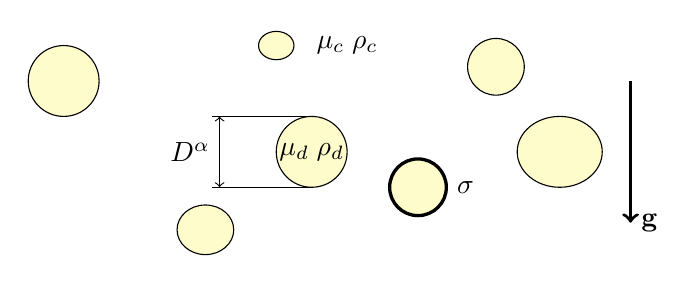
\begin{tikzpicture}[scale = 0.9]
        \draw[fill=yellow!20](3,3) node{$\mu_c\;\rho_c$};
        \foreach \x/\y/\ra/\r in {2/3/0.2/0.25,
        5.1/2.7/0.4/0.4,
        1/0.4/0.35/0.4,
        4/1/0.4/0.4,
        6/1.5/0.5/0.6,
        -1/2.5/0.5/0.5}{
            \draw[fill=yellow!20](\x,\y) ellipse(\r cm and \ra cm);
        }
        \draw[fill=yellow!20](2.5,1.5) circle(0.5)node{$\mu_d\;\rho_d$};
        \draw[thin,-](1.1,2)--++(1.4,0);
        \draw[thin,-](1.1,1)--++(1.4,0);
        \draw[very thick,black!80!black](4,1) ellipse (0.4cm and 0.4cm);
        \draw[very thick,black!80!black](4,1)++(0.4,0)node[right]{$\sigma$};
        \draw[thin,<->](1.2,1)--++(0,1)node[midway,left]{$D^\alpha$};
        \draw[very thick,->](7,2.5)--++(0,-2)node[right]{$\textbf{g}$};
    \end{tikzpicture}
    \caption{Scheme of droplets immersed into a continuous fluid phase.}
    \label{fig:scheme}
\end{figure}

There is a total of $9$ independent physical parameters to this problem (if we consider only the mean of the sizes $D$), they are all constituted by 3 fundamental units, a length, a mass and the time.
Therefore, according to Buckingham $\Pi$ theorem we can define a minimum of $9-3 = 6$ dimensionless numbers to describe the problem. 
Several options are available the selection is somewhat arbitrary, so we choose the following set of dimensionless numbers. 
The $4^{th}$ first parameters are linked to the physical properties of the emulsion, namely, 
\begin{align*}
    & Ga^2 =\frac{\rho_c(\rho_c - \rho_d) g D^3}{\mu^2_c}& 
    & Bo =\frac{(\rho_c - \rho_d) g D^2}{\sigma}&
    & \mu_r = \frac{\mu_c}{\mu_d}& 
    & \rho_r = \frac{\rho_c}{\rho_d}&
\end{align*}
And the two remaining parameters are related to the topology of the flow, 
\begin{align*}
    \phi = \frac{V_d}{V_c} & &
    N_b = \frac{6V_d}{\pi D^3}
\end{align*}
with $N_b$ is the number of droplets in the volume considered and $\phi$ the volume fraction of the dispersed phase.
The \textit{Galileo number} or \textit{Archimedes number}, is the ratio of the buoyancy forces over the viscosity forces, noted $Ga$.
Note that the \textit{Reynolds number}, defined by, $Re = \rho_c L U/\mu$, where $U$ is the characteristic velocity, is equivalent to the \textit{Galileo number} if we take $U = \sqrt{gL(\rho_c-\rho_d)/\rho_c}$ as the velocity scale.
$Bo$ is the \textit{Bond} or \textit{E\"otv\"os number}, it is the ratio between the buoyancy forces and surface tension forces. 
Notice that $We = Bo/Ga^2$, with $We$ the \textit{Weber number} compares the viscous forces with capillarity forces.
Thus, $We$ describe the deformation of the droplets, as an example, above a critical value of the \textit{Weber number} a droplet will break due to hydrodynamical forces \citet{deike2022direct}. 
Lastly, $\mu_r$ and $\rho_r$ are respectively the density and viscosity ratios. 

To give a brief idea about the range of interest of those numbers in the industrial context, we take the example of an oil/water emulsion.
In the real processes the diameter of the droplets lies in the range $D = [10 \mu \text{m}, 1 \text{mm}]$.
The density and viscosity of water are approximately $\rho_c = 1000 \text{kg/m}^3$ and $\mu_c = 10^{-3}$.
The density and viscosity of oil are close to $\rho_d = 900 \text{kg/m}^3$ and $\mu_d = 10^{-2}$.
We consider the gravity acceleration on earth, thus it is $g= 9.81 \text{kg.m.s}^{-2}$.
The surface tension of the system oil/water is known to be approximately $\sigma = 50 \text{mJ/m}^2$ \citep{de2015gouttes}. 
We display the values of dimensionless parameters computed with those physical parameters in \ref{tab:parameters}.
\begin{table}[h!]
    \centering
    \caption{Dimensionless parameters for a water/oil emulsion.}
    \begin{tabular}{|c||c|c|c|c|c|}
        \hline&$Ga$&$Bo$&$\phi$&$\mu_r$&$\rho_r$\\ \hline
        \hline Oil/Water&$[0.03,30]$&$[10^{-6};10^{-2}]$&$[0,0.15]$&$0.1$&$1.111$\\ \hline
    \end{tabular}
    \label{tab:parameters}
\end{table}
We can notice that the \textit{Galileo number} is rather low therefore can already state that it will be necessary to investigate the stokes flow limit. 
Likewise, The \textit{Bond number} is very low, meaning that the droplets are nearly spherical.
Consequently, in the following models and numerical simulations we must consider some cases with spherical particles. 
The viscosity and density ratio as well as the volume fraction do not permit any additional assumption on the flow. 

\section{Current state of dispersed two-phase flow  modeling}

Up to now a lot of investigations have been made on the modeling of bubbly flows.
Indeed, bubbly flows are of large interest since they appear in plenty applications (especially the nuclear industry).
Consequently, researchers have been trying to find closure terms on the specific case of bubbly flows. 
For these reason, most of the studies cited below investigate bubble hydrodynamics (and not droplets). 
Also, in the perspective of modeling the reactor scale authors have developed software carrying out Euler-Euler simulations. 
The most famous ones are NEPTUNE-CFD belonging to EDF, and OpenFoam with its collection of multiphase solvers. 
Again, most of the authors carried the computation of the averaged equations of bubbly flows and not emulsion.
Even though in this thesis we solely focus on the closure terms calculation, it is of interest to say a few words on the modeling of the upper scale.
i.e. the industrial scale, where we solve the averaged equations derived in \ref{chap:avg}. 

\subsection{Macro scale modeling with CFD-PBM}
Here is a brief review of the authors who attempted to carry out CFD-PBE simulation.
\citet{wang1995simultaneous} study numerically the PBM equations for buoyancy-driven setting of spherical drops suspension.
They consider a one-dimensional PBE for the axis along the column. 
And solve for the continuous size distribution function $f$.
The source terms $B(n)$ are modeled using the theoretical formulas depicted in the previous chapter, and the probability of coalescence is assumed to be 1 since there is no bouncing in the absence of inertia (therefore a contact results always in coalescence). 
In this context, they could solve the equations, and they show how the coalescence influences the phase separation inside a vessel.
In \cite{KAMP20011363} they solve numerically the averaged PEB considering one dimensional and spherical bubbly flow.
They solve the first and second-order equations of the PBE.
They also considered the velocity of the bubbles as independent of the bubble size. 
The coalescence kernel is derived for unequal bubble size interaction in turbulent flows. 
The results are validated with experimental data on pipe flows under microgravity conditions. 
They could show that the coalescence rate diminishes between the inlet and outlet due to the decrease in the rate of collision because the velocities of collision are higher. 

Next,  \citet{morel2010comparison} performed simulations of Euler-Euler models coupled with PBE for bubbly flow columns. 
They considered 4 different situations with different hypotheses, namely, the single-size approach, the moment approach based on the log-normal distribution, the moment approach based on the quadratic law, and the multi-fields approach.
The latter method is also called the class method mentioned in the previous chapter (it consists of solving the N equations for the mass and momentum of the N class of particles).
They conclude that from the first to the last method the accuracy increased together with the numerical cost.
Apart from the last method which is completely different from the others and turns out to over-predict coalescence. 
Now, in \citet{gemello2018modelling} a full CFD-PBM is modeled for bubbly column on the code \texttt{OpenFoam}. 
The CFD part is modeled with the averaged Navier Stokes equation.
They use classic turbulence model (i.e. $k-\varepsilon$ model, RNG $k-\varepsilon$ and $k-\omega$ model) to account for the velocity fluctuation term, $\left<\bm{u}'\bm{u}'\right>^f$. 
They conclude that $k-\omega$ was the most practical model in terms of accuracy and stability.
\citet{alam2022cfd} conducted CFD-PBM and experimental study on a nano-bubble generator. 
They also compared different turbulence models and found out that the $k-\omega$ model predicted a better prediction for high flow rates.
Note that this modeling of the pseudo-turbulent tensor is not physical as pseudo-turbulence is different from classic turbulence.
A slightly different work is done by \citet{salehi2017population}, they coupled Large Eddy simulation to PDF-PBM to predict the distribution shape and size of droplets in atomization turbulent flows. 
The dispersed phase is here modeled with a Lagrangian approach, the drag force term uses the mean velocity difference between the averaged continuous phase and the dispersed phase.
The additional feature of this work is that they take into account the size and the shape as variable in the droplet distribution.
The strategy of stokes binding is used here, this method consists in representing one notional particle for a particle size.

Though, all the processes modeled by these authors involve poly dispersed two-phase flow, none or few of them, are considered accurate closure for the velocity fluctuation (they often consider turbulence-like models) and the other first order moments closures terms are neglected. 
The reason is that no accurate closure terms exist yet in the literature. 
Only the drag forces seem to be predicted from robust semi-empirical correlations, for bubbly flow at least.

\subsection{DNS modeling of suspended particles or droplets}

Now, let's focus on the numerical studies providing empirical expression for the closure terms. 
Numerous authors worked on the topic, and most of them are already mentioned in the previous chapter regarding their theoretical work. 
Note that all the following articles are rather recent since DNS of bubbly flow is quite expensive and has been achievable for only a few years. 
\citet{esmaeeli2005direct} carried out  DNS of representative periodic volume of bubbly flow. 
They measure the rising velocity, velocity fluctuation as well as the relative orientation of the pair of bubbles.
Furthermore, they could predict the averaged rising velocity reasonably well, as it is the simplest quantity to predict among all the closure terms.
Indeed, the rising velocity is the quantity that converges faster than the other thus less sample is needed to predict it.
At the time they were limited by computer performances, thus, the maximum Reynolds number archived is $Re  = 77$, indeed more grid points are needed for higher $Re$. 
They simulated deformable and non-deformable bubbles.
The main difference is that the spherical bubbles form \textit{raft} where the arrangement of the deformable bubbles is pretty random. 
They also found a Gaussian distribution for the velocity fluctuation.
In a more recent work \citet{willen2019resolved} simulated equal spheres in an upward flow.
They also compute the velocity and velocity fluctuation and show that the suspension was anisotropic in the direction of the gravity force.
Besides, they also measured the structure of the flow and recovered the column arrangement and horizontal arrangement, to analyze the structure they used tetrads which allowed them to see the evolution of the relative positions.
\citet{du2022analysis} perform DNS calculation of mono disperse bubbly flow and focus on the calculation of pseudo turbulent tensor. 
They separate the pseudo turbulence tensor into two contributions.
The wake-induced turbulence and the potential flow and averaged wake fluctuation.
The former is the main focus of the study and a model is proposed.
% All these studies used DNS and analyzed the closure by computing it directly.
% However, other authors considered wave analysis to get the closure terms. 
% We won't go into details, but it is possible to compute several closures by the analysis of the wave speed.
% For more information we point the reader to the following articles,  \cite{duru2002constitutive}, \citet{willen2017continuity} and\citet{derksen2007direct}.
On another hands \citet{wang2021numerical} performed DNS of a random array of fixed spherical particle.
About 3000 spheres were modeled to get a representative sample. 
They computed the PFP stress based on the nearest particle statistic.
They show that this particle stress can predict the skewing effect along the flow direction and repealing effects on the normal directions of the particular phase. 
This is the only study reporting the calculation of the PFP stress therefore a need is clearly needed on this matter.
\citet{manga1995collective} studied experimentally as well as numerically, with boundary integral methods, the rate of coalescence of interacting pairs of drops.
They investigated the influence of deformation on the rate of coalescence and concluded that the greater the drops or bubble deform (for high $Bo$ and  $Ga$) the higher the probability of coalesce will be (might go up to one order of magnitude above than for non-deformable drops).
It also results in a wider distribution of the particle size.
\citet{innocenti2020direct} simulated 3D column of rising bubbles and evaluated velocity fluctuation and energy dissipation for turbulence. 
\citet{hidman2023assessing} simulated tri-periodic simulation of rising mono-dispersed bubbly-flows. 
Interestingly their simulations'  setup is close to what we wish to accomplish. 


From all the studies presented above it seems that getting the closure terms through DNS seems well achievable.
The most suited setup in our case seems to be the simulation of random arrays of bubbles, similarly to \citet{hidman2023assessing}.
Indeed, they could measure the velocity fluctuations properly and other closures like the drag forces (through the averaged velocity) and also terms related to turbulence modeling and transport of passive scalar. 
Additionally, to avoid the modeling of a large domain they make use of periodic boundary conditions, which is what we will do.
This way we will be able to provide closure terms for buoyant driven emulsion.
In the next section, we present the methodology to carry out massive DNS of a tri-periodic random array of rising drops.



\section{Basilisk a suited software to perform massive DNS calculations.}

In view of the previous research (especially the study of \citet{innocenti2020direct}) and the good results obtained in \citet{Naanouh2021numerical}, we thought that the partial differential equation solver, Basilisk (from \url{basilisk.fr}), was the most suited code to carry out tri-periodic simulation of buoyant droplets. 
Originally this code is based on the older code,  \texttt{Gerris}, and was developed primarily by Francesco De Vita, Jose-Maria Fullana, Geoffroy Kirstet-ter, Pierre-Yves Langrée, Emily Lane, Jose Lopez-Herrerra, John MacFarlane, Stéphane Popinet, Clément Robert, and Antoon van Hooft .
Both codes are open source, that is why since then the community contributed to the development of Basilisk and numerous authors published their contribution to the code in scientific reviews.
The open source aspect of Basilisk is somewhat essential for us since it enable us the to develop any desired features.
Besides, a lot of benchmarks demonstrated the good performances and the broad abilities of Basilisk.
All the algorithms are developed in C, if well done this language has the great advantage of optimizing the memory management, resulting in a better computation efficiency. 
Moreover, a lot of physical solvers are already implemented in the code, from wave modeling \citet{mostert2022high} to the simulation of suspended solid particles in a fluid using immersed boundary method \citet{shui2015direct}.
A last feature that has been recently implemented in Basilisk is the multilayer solvers \citep{popinet2020vertically} which will be of great interest in the modeling of film drainage problems. 
We refer the reader to this link \url{http://basilisk.fr/src/README} to see the whole range of possibilities offered by Basilisk.
Nevertheless, the most interesting feature for our use is the capability of modeling two phase flow in Basilisk. 
Indeed, the Volume-Of-Fluid (VOF) method implemented in Basilisk have shown great performance and accuracy, (see \citet{popinet2009accurate}\citet{popinet2018numerical}). 
This point will be developed in a following section since it is of major importance. 
Another practical aspect of Basilisk is that the meshing is included in the workflow of the simulation. 
This enables the possibility of switching between 2D cases and 3D cases automatically, indeed the \textit{dimension} parameter need to be switch from 2 to 3 the rest is automatic. 
In our case it is of a great use since we will start by carrying out 2D simulations and after validation we will switch to 3D mesh.
Speaking of the mesh, Basilisk provide several mesh types that considerably improve the efficiency of the calculation.
The first one is the classic Cartesian mesh, it is fully orthogonal, this is the most for mono-scale problem.
Another interesting grid is the adaptive mesh, as indicate by its name this mesh refines the area where high velocity gradients is observed.
\citet{innocenti2020direct} model a large quantity of bubbles in a container, this was only possible thanks to the adaptive mesh solver, otherwise it would have been too expansive.
The simulation of wave crashes by, \citet{mostert2022high} was made possible also thanks to the adaptive mesh refinement.
Numerous other examples testify of the usefulness of the adaptive mesh refinement solver.   
Then the last meshing technics is a subcase of the adaptive mesh, it is the \texttt{multigrid} mesh, presented in \citet{popinet2003gerris} for the incompressible Euler equations, and more recently in \citet{popinet2015quadtree} for the fully-nonlinear Boussinesq wave equations. 
This meshing technics consist in working with different levels of refined grids simultaneously.
More details will be given about the meshes in this section. 
Finally, the last point on which we would like to emphasize is that Basilisk is a self independent software (i;e. Only the source code of basilisk is needed to compile it) and simulations are launch via C files. 
Which makes it practical for the execution on any machines (cluster or not). 
In the next sections we present the specificity of the VOF methods, needs we speak more specifically about our numerical setup to model rising suspension of droplets. 



\subsection{The Volume Of Fluid Method}

The VOF method is used to model two-phase (or more) flows. 
The governing equations, solved by our solver in the present case, are the one-fluid formulation equation of momentum and mass, presented in \ref{chap:avg}. 
We recall their form here, 
\begin{equation}
    \pddt (\rho \textbf{u})
    = \nablabh \cdot (\textbf{T} -\rho  \textbf{u} \textbf{u})
    + \textbf{b}
    + \textbf{f}_I\delta_I
    \;\;\;\text{and}\;\;\;
    \pddt \rho
    = 
    - \nablabh\cdot(\rho\textbf{u}_k). 
\end{equation}
Note that the material properties (i.e. $\rho$ and $\mu$) takes the value of the phase in presence. 
As seen in \ref{chap:avg}, in two phases flows we define a phase indicator function $\chi$, which is a marker to identify the phases in presence.
When, $\chi = 1$, we are located in the dispersed phase, when $\chi = 0$ in the fluid phase for example, therefore $\chi$ correspond to a Heaviside function. 
However, the Heaviside function is not continuous and derivable everywhere. 
This latter point makes the use of $\chi$ impossible in numerical method.
Therefore, in CFD code, we use an approximation of the Heaviside function, namely the color function $C$. 
Since we want to follow the phases with time,  we need to add the equation of transport of $C$ to complete the system, namely,
\begin{equation}
    \frac{\partial C}{\partial t} + \textbf{u}\cdot\bm{\nabla} C = 0.
    \label{eq:cfunc} 
\end{equation}
At this point several methods are available to define $C$ and to discretize these equations. 

Regardless of the definition of $C$ it is important to say a few words on the discretization of the Navier-Sokes equations which is independent of this choice. 
Basilisk uses the finite volume based method to discretize the governing partial differential equations.
A full review of the finite volume method is made in the book \citet{ferziger2002computational}.
The finite volume method consists in discretizing the whole domain of fluid by finite volume called cells. 
This discretized domain is what we call a mesh. 
In Basilisk we use only orthogonal meshes. 
Which means that the cells of the domain are only squares or cubes.
Nevertheless, as mentioned in introduction there are several specificities among these orthogonal grids.   
\begin{figure}[h!]
    \centering
    \begin{tikzpicture}
        \node (a) at (-0.25\textwidth,0){
\includegraphics[height = 0.2575\textwidth]{image/pic/Uniforme.png}};
        \node (b) at (0,0){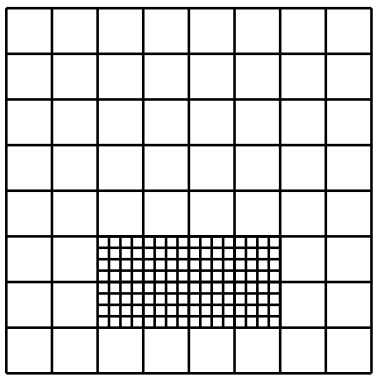
\includegraphics[height = 0.25\textwidth]{image/pic/non-uniform.png}};
        \node (c) at (0.25\textwidth,0){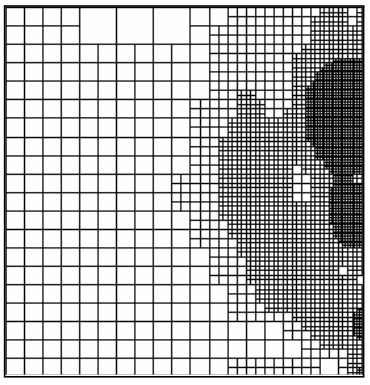
\includegraphics[height = 0.25\textwidth]{image/pic/adaptativemesh.png}};
        \node (leg) at (a.south){(a)}; 
        \node (leg) at (b.south){(b)}; 
        \node (leg) at (c.south){(c)}; 
    \end{tikzpicture}
    \caption{Different type of orthogonal meshes. (a) uniform mesh, (b) Non-uniform mesh, (c) Adaptive \textit{Quad/Octree} mesh. Reprinted from \citet{mani2021numerical}. }
    \label{fig:meshes}
\end{figure}
The first one is the classic uniform grid depicted \ref{fig:meshes} where all the cells have the same size.
The second one is the non-uniform grid. 
It is useful when the user need to refine a specific area of the mesh, due to high local gradient of the velocity for example.
Then, the last one, is the Adaptive \textit{Quad/Octree} Grids, on which we are to give a bit more details.
It consists in subdividing the cells into $2^2$ cells in two dimension, or in $2^3$ cells in 3 dimension. 
Each cell that have the same size form a group.
All the groups are referred by their respective \textit{levels}. 
The group of level 0 is the one with the larger cells size, actually at this there is only one cell of the size of the domain. 
Then as we look at higher levels the size of the cells decrease. 
Besides, Basilisk offer the possibility of the \textit{Adaptive} option. 
Which means that the cells are subdividing or merging themselves automatically all along the simulation time. 
At the frontier between two levels there is what we called the \textit{resolution boundary}. 
Those boundaries, are somewhat problematic since the cells on each side are not of the same size.
Therefore, the basic operation of the finite volume method are not trivial anymore. 
To avoid this issue Basilisk use \textit{halo cells}.
One \textit{halo cell} is the representation of the cell of the lower level that gather the mean value of the four smaller cells.
The former cell is of the same size of the cell at the other side of the \textit{resolution boundary}, that is why the system is consistent. 
In Basilisk the cells from which the \textit{halo cells} are build are called the children cells, therefore the lower level cells are the parent cells. 
This principle is used for the adaptive mesh, nevertheless, the \textit{Quad/Octree} grid has one subclass, the \textit{multigrid} mesh. 
This meshing technics is no more than a uniform mesh where we make use of the \textit{halo cells}, and parent/children principle. 
Even though there is no \textit{resolution boundary}, this technics allows the user to loop through different levels and through each branch of the mesh. 
This feature is of a great interest to carry out fast operations on vector or scalar fields. 
We refer to the publication of \citet{popinet2015quadtree} for a more detailed explanation.  
Once the mesh is set one need to discretize the governing equations in space and time (see \citet[chapter 3]{tryggvason2011direct}). 

Five main option exist to define the color function $C$ :
the volume of fluid method,
the front taking method,
the level-set method,
the phase-field method
and the CIP method.
As the title of this section is the \textit{volume of fluid method} one could guess which one we use. 
For more details on the other methods we refer the reader to \cite[Chapter 4]{tryggvason2011direct}. 
With the Volume-of-fluid method the color function is now defined by a \textit{VOF tracer}, $f_i$, where $k$ stand for the indices referring to the phase. 
For $N$ VOF tracer $f_k$ is defined for $0\leq k\leq N$.
From $k=0$ for the continuous phase to $k=1$ to $N$ for the dispersed phases (in case we have $N$ dispersed phases). 
In practice the function $f_c$ is not computed since we have the relation, $f_c = 1- \sum_{k=1}^N f_k$. 
The value of the $f_k$ is comprised between $0$ and $1$.
$f_k = 0$ meaning that the concentration of phase $k$ is null, $f_k = 1$ meaning that $100\%$ of the volume is occupied by the phase $k$. 
Note that in every cell the value of $f_k$ is either $0$ or $1$, except in the cells including an interface where the value is the percentage of the phases in presence.
\begin{equation}
    f_k = \left\{\begin{tabular}{cc}
        $1$  &if $\textbf{y}\in V_k$\\
        $0$  &if $\textbf{y}\in V_c$\\
        $0$ to $1$  &if $\textbf{y}\in V_c \cap V_k$\\
    \end{tabular}
    \right.,
\end{equation}
where $V_k$ is the volume occupied by the phase $k$.
The overall condition is that $\sum_k^N f_k \leq 1$.
Next, if we note $\rho_k$ and $\mu_k$ the material property of phase $k$ we can finally compute in each cell the value of the material properties,
\begin{equation*}
    \rho 
    = \sum_k^N \rho_k f_k 
    + (1-\sum_k^Nf_k)\rho_c 
    \;\;\;\text{and}\;\;\;
    \mu 
    = \sum_k^N\mu_k f_k 
    + (1-\sum_k^Nf_k)\mu_c.
\end{equation*} 
In the neighboring cells of the interfaces the calculation of $\rho$ and $\mu$ are slightly different \citep{tryggvason2011direct}. 
Then, once the material properties are calculated, the Navier-Stokes equations solved and the VOF tracers advected, the last step is to reconstruct the interfaces from the $f_k$.
To do so, several methods, more or less accurate, are available  to us.
\ref{fig:VOF} depicts the different reconstruction method, namely, the Simple Line Interface Calculation or SLIC method, the Hirt and Nichols reconstruction method and the Piecewise Linear Interface Calculation or PLIC method. 
As we can clearly see on the scheme the methods goes from coarse (with SLIC) definition of the interface to a more accurate reconstruction (with PLIC).
\begin{figure}
    \centering
    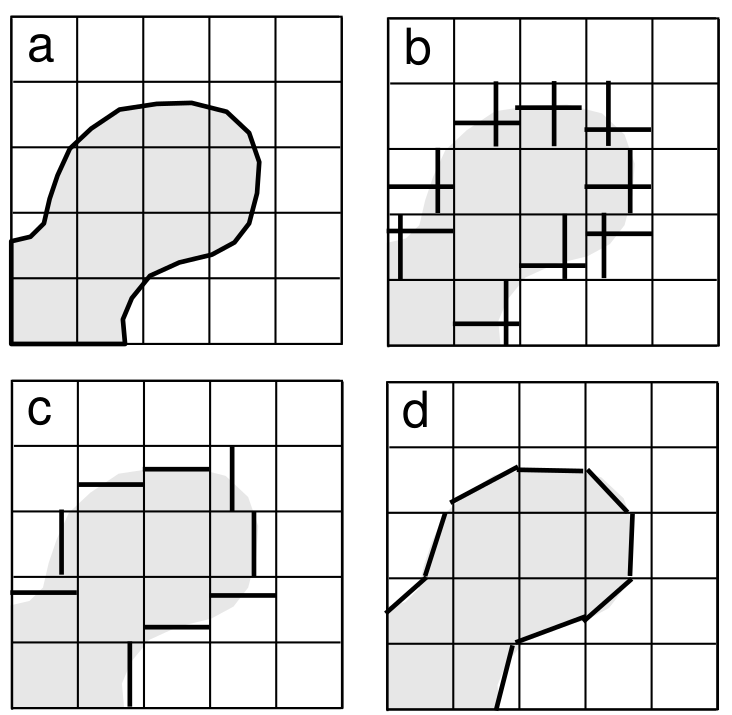
\includegraphics[width = 0.4\textwidth]{image/pic/VOF.png}
    \caption{VOF reconstruction of the solution for advection in two dimensions. 
    (a) The original interface. 
    (b) The original SLIC reconstruction. 
    (c) The Hirt and Nichols reconstruction. 
    (d) PLIC reconstruction. 
    Reprinted from \citet{tryggvason2011direct}.}
    \label{fig:VOF}
\end{figure}
In Basilisk we use PLIC method using height functions (see \citet[Chapter 5]{tryggvason2011direct}). 
Here is a quick summary of how height functions work.
Each segment is parametrized by its normal $\textbf{n}$ and the intercept of a line, $\alpha$. 
Then, in the local reference frame of coordinate $\textbf{z}$, it is possible to define the interface by,
\begin{equation}
    \textbf{n}\cdot\textbf{z} 
    = \alpha,
\end{equation}
where $\alpha$ is computed with the local volume fraction of the phase and the unit normal. 
The overall error is of second order. 
Nevertheless, it must be said that even though the PLIC method is accurate, it still has some draw back sheared with the two other methods. 
Indeed, if we consider 2 tracers the interface is reconstructed considering the tracer $f_c$ and the tracer $f_1$.
Which is equivalent to consider two phases, up to now everything is normal. 
But, consider two interfaces getting closer, then at some point the interfaces will merge together discarding the physical aspect.
Indeed, since we compute height functions from the local volume fraction, if two drops with the same tracer met, then the interfaces are reconstructed regardless of the physical geometry. 
Another problem is that VOF tracers are advected separately so interpenetration of different VOF tracers can happen (this issue will be developed in the next section). 
These two facts mandate the use of a relatively fine mesh so that the film between the droplets is partially resolved.

Once the interface is reconstructed, we can tackle the most challenging problem of VOF simulations.
Which is the modeling of the surface tension forces, i.e. the source term, $\textbf{f}_I\delta_I$, in the one-fluid formulation equations.
Obviously we will not detail the solutions here, to get an overall vision of the problem we refer the reader to \citet{popinet2018numerical} or  \citet[Chapter 7]{tryggvason2011direct}.
However, we can cite the two most basic method.
The first one is the \textit{Continuous surface force method}, in consist in discretizing the expression of the surface force source term. 
Note that the expression of $\delta_S$ make use of the color function, it is in fact equal to the gradient of the color function. 
The approximation of the surface force source term is then,
\begin{equation}
    \sigma \kappa  \textbf{n} \delta_I 
    = \sigma \kappa \nabla f_i,
\end{equation}
where the curvature $\kappa$ is estimated through height function \citep{popinet2018numerical}. 
The other method is the \textit{Continuous surface stress method} which is equivalent, but instead of discretizing the force term, we discretize the divergence of a stress.
It reads, 
\begin{equation}
    \textbf{f}_I \delta_I = \nabla \cdot \left[\sigma (\textbf{I}-\textbf{nn})\delta_I\right],
\end{equation}
\tb{Find were does that came from}
which is valid even with non-constant $\sigma$. 
In Basilisk, we make use of the former method. 

The overall difficulty encountered in the two-phase flows simulations is to manage the singularities at the interfaces.
Indeed, it is a common problem in mathematic when the function is not derivable everywhere.
Hence, from a numerical point of view it is no less of a problem. 
In the conclusion of this chapter we will review some issues arising in  the simulation of emulsion because of this point. 

\subsection{Numerical coalescence}

As briefly mentioned in the preceding section, numerical coalescence can occur during a simulation if two interfaces are one cell mesh apart (assuming there is a solely VOF tracer). 
However, in \ref{chap:avg} we showed that the coalescence of two droplets is a multiscale phenomenon. 
At first, it involves hydrodynamical and lubrication forces.
Once the interfaces are close enough Van deer Waals forces are responsible for the coalescence.
The former forces are well modeled when using a fine enough mesh. 
Indeed, we solve the Navier-Stokes equation together with the transport of the color function, which is the basis of the calculation of the lubrication forces \citep{guazzelli2011}. 
However, the latter contribution involve microscale interaction which are not included in this model.
Even though, it is possible to include Van der Waals forces in Basilisk, it would be too expensive to compute the film drainage problem for several droplets at the same time.
To avoid this problem \citet{thomas2010multiscale} modeled the film drainage by allowing coalescence when the contact time of the droplet is greater than the critical time of contact (computed theoretically).  
However, the closure for the contact time is not well define for our parameters yet.
Moreover, before allowing coalescence after a critical time, we need to prevent it anyway. 
Hence, in any cases we need to prevent coalescence event to happen since DNS of the film drainage is too expansive numerically. 
Besides, to create accurate closures terms seen in \ref{chap:avg}, we need to identify accurately the topology of a given situation.
This way we will be able to give the value of a closure term in terms of the exact number and size of the droplets for example. 
This implies that we must keep a constant number of droplets all along the simulation.

Before avoiding coalescence to happen it is important to identify why it does happen. 
The reason why numerical coalescence occurs is that only one VOF tracer is used. 
Indeed, let's take two drops approaching each other. 
The VOF tracer is advected along the velocity fields. 
We recall that in the interfacial area the VOF tracer has a transitional value between $1$ and $0$. 
Therefore, when the drops eventually get close enough the VOF tracer at the interface of the drops meet each other in the same cells. 
Since the same VOF tracer is used for the two droplet, it results in the addition of the values of the VOF tracer at the interfaces since they gather in the same cells. 
Then, as the VOF tracer merge it is impossible to reconstruct the interface of the respective droplets. 

Using different VOF tracer would prevent the drops to coalesce 
Indeed, during advection the VOF tracer will not sum with the neighboring ones thus the reconstruction of the interface will be possible. 
However, in the literature, we see that we need about hundreds of particles to be able to get a representative volume. 
And since we need to advect each VOF tracers independently, it would be too expensive to have one VOF tracer per drops.    
Luckily, we only need that the adjacent droplets at a given time $t$ have different VOF tracer. 
In 2D the famous \textit{four color map theorems} stipulate that we only need 4 color to color adjacent country with a different color (this is a topological proof).
For our concern, it does mean that we will need no more than four VOF tracer in order for the adjacent droplets to have different VOF tracer. 
In 3D this theorem is not valid anymore. 
Moreover, the droplets move within time thus their neighboring particles changes, and they might need a different VOF tracer.

To tackle this issue \citet{mani2021numerical}, developed an algorithm on Basilisk to carry out the previous task automatically. 
Even though, this algorithm is based on empirical observation and not topological arguments it prevents from using too much VOF tracer. 
The workflow is as follows.
In a first step we identify the VOF tracer having droplets that are close to each other. 
Then for each of these VOF tracers, we identify the pairs of droplets. 
Then we check which of the droplets among one pair have the least neighbors. 
Finally, we switch the VOF tracer of the former droplet to a new tracer that is not in the vicinity of the droplet. 
If no VOF tracer is available then we create a new one. 
In the practical case we indeed notice that 2D simulations do not use more than 4 VOF tracers. 
Therefore, this is a proof of the efficiency of the algorithm. 
This algorithm considers a droplet close to another one only if they have VOF tracers two cells apart.
Consequently, if the drops relative velocity is greater than that this length time the time step then the algorithm will not work.
Nevertheless, in practice the CFL condition is respected which means that the distance traveled by a fluid particle is never superior to one mesh cell. 
This algorithm is launched every time step by default, nevertheless we could call it every 2 time steps (since three would be a bit reckless). 
\tb{more details on this matter }
\subsection{Simulation of periodic rising droplets}
As concluded in the two previous sections, we are going to make DNS of a random array of droplet rising in a continuous Newtonian fluid with the code Basilisk. 
Therefore, in this section we are going to present the 


In Basilisk the computational domain of the simulation must be a square in 2D or a cube in 3D, as depicted on \ref{fig:numscheme}. 
Depending on the desired number of bubbles $N_b$ we divide the domain of size $\mathcal{L}$ in $N$ smaller squares of length $\Delta$.
In each smaller squares we initialize the VOF tracers $f_i$ as a spherical, in 3D, or circular, in 2D, shaped area representing the droplets.
Each droplet of diameter $L$ is centered inside their $\Delta\times \Delta$ square.
Besides, we add a random shift vector for each droplet position so that all the simulations with the same parameters are unique. 
The shift must be limited in order to avoid that the drops touch each other at the initialization time (in which case they would immediately merge).   
Also, another method consist of initializing all droplets randomly, making sure that they are initially far enough so that they do not touch each other at the first step of the simulation.
The latter technics was used in the simulation performed in \ref{chap:mono-disperse} since it has shown faster convergence. 
Indeed, as we initialize with a random state, the suspension takes a shorter amount of time to reach it statistically random steady state. 
\begin{figure}[h!]
    \centering
    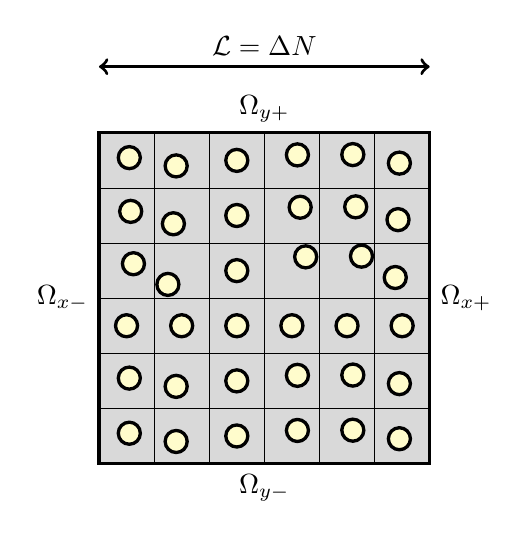
\begin{tikzpicture}[very thick,scale = 0.7]
        \draw[fill=gray!30](0,0) rectangle(6,6);
        \foreach \x/\dx in {0.5/0.1,1.5/-0.2,2.5/0,3.5/0.2,4.5/0.21,5.5/-0.1}{
            \draw[very thin](\x+0.5,0)--(\x+0.5,6);
            \draw[very thin](0,\x+0.5)--(6,\x+0.5);
            \foreach \y/\dy in {0.5/0.1,1.5/+0.1,2.5/0,3.5/0.25,4.5/0.15,5.5/0.1}{
                \draw[fill=yellow!20](\x+\dx*\dy*5,\y+\dy*\dx*5) ellipse(0.2 cm and 0.2 cm);
            }
        }
        \draw[<->](0,7.2)--(6,7.2)node[midway, above]{$\mathcal{L} = \Delta N$};
        \draw(3,6)node[above]{$\Omega_{y+}$};
        \draw(3,0)node[below]{$\Omega_{y-}$};
        \draw(6,3)node[right]{$\Omega_{x+}$};
        \draw(0,3)node[left]{$\Omega_{x-}$};
    \end{tikzpicture}
    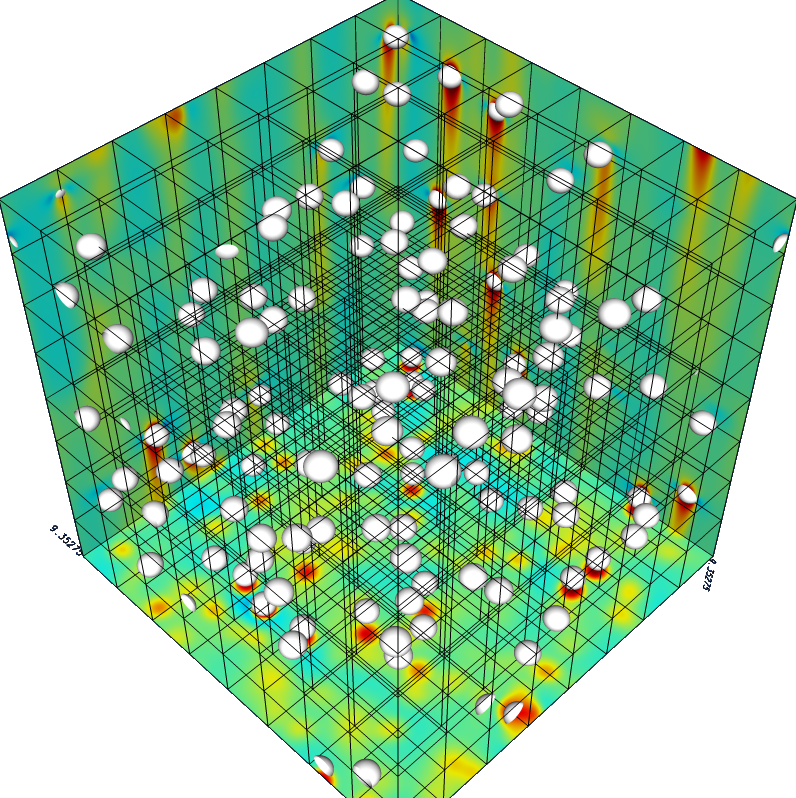
\includegraphics[width=0.45\textwidth]{image/3D/PHI01.png}
    \caption{(left) Scheme of the initialization of an array of droplets immersed in a 2D periodic domain.
    (right) Picture of a 3D simulation with $\phi = 0.1$, $N = 5$ the color represent the velocity field.}
    \label{fig:numscheme}
\end{figure}

The dimensionless parameters of this study have been already discussed in \ref{chap:avg}.
Nevertheless, additional dimensionless parameters must be introduced since numerical parameters that weren't on the theoretical problem appear. 
Only six parameters are needed among the existing dimensionless parameters. 
However, the numerical simulations involve an others length parameters among the ones already mentioned in \ref{sec:introavg}, namely the length of a cell in the mesh.
Therefore, we need to define a new dimensionless parameter, namely, the number of cells per diameter refer by $\delta$. 
From those parameters it is possible to recover the physical parameters needed by the simulation. 
But before we fix the following parameters, $\rho_d = L = g = 1$ for convenience.
Then it yields the following relations to recover the remaining parameters,
\begin{align*}
    &\rho_c = \rho_d\rho_r ,&
    &\mu_d  =\frac{\rho_d \sqrt{|1-\rho_r| \rho_r g \bar{L}^3}}{\mu_r Ga},&
    &\mu_c  = \mu_d\mu_r,&
    &\delta  = D/Nc& \\
    &\sigma = \frac{|1-\rho_r|\rho_d g L^2}{Bo},&
    &\Delta = \sqrt{\frac{\pi D^2}{4\phi}},&
    &\mathcal{L} = \Delta \sqrt{N_b}.&
\end{align*}
From those parameters it is possible to define different time, length and velocity scales. 
It will be useful when we will need to make the results dimensionless. 
The different scales in which we will be interested in are the following.
\begin{align*}
    &U_\mu = \frac{g D^2 \Delta \rho}{\mu_c}&
    &U_\rho = \sqrt{\Delta \rho \frac{Dg}{\rho_d}}&
    &U_\sigma = \sqrt{\Delta \rho \frac{Dg}{\rho_d}}& \\
    &T_\mu = \frac{\mu_c}{g\Delta \rho D}&
    &T_\rho = \sqrt{\frac{\rho_dD}{g\Delta\rho}}&
    &T_\sigma = \sqrt{\frac{\rho_{avg} D^3}{\pi \sigma}}&
\end{align*}
Were $U_\mu$, $U_\rho$ and $U_\sigma$ are respectively the viscous inertial and capillary velocity scales. 
Similarly, $T_\mu$, $T_\rho$ and $T_\sigma$ are the corresponding time scales. 
Here is a quick explanation of the physical meaning of those scales :
When $Ga \ll 1$, in one unit of $T_\mu$ a droplet travel a distance of $D$ relatively to the fluid.  
Similarly, When $Ga \gg 1$ a droplet travel a distance of $D$ in one unit of $T_\rho$. 
Lastly, the Capillary time $T_\sigma$ will be the period of one undulation of the surface droplet. 
Of course this scale provide us with an order of magnitude, they aren't exact. 

In Basilisk the set-up of a simulation (solvers and parameters) is made by including or excluding header files.
All the header files can of course be found in the sources of the code (\url{http://basilisk.fr/src/}).   
In the following, we describe the header files used in this simulation. 
The first one has in fact already been mentioned, it is \href{http://basilisk.fr/src/grid/multigrid.h}{multigrid.h} or  \href{http://basilisk.fr/src/grid/multigrid3D.h}{multigrid3D.h} file for 3D simulations. 
It set up a uniform staggered multigrid mesh. 
Then, we add the file \href{http://basilisk.fr/src/navier-stokes/centered.h}{centered.h} to resolve Navier Stokes equation on this mesh with centered formulation.
The \texttt{two-phase.h} header set up the VOF tracers and interfaces for two immiscible fluid.
It also set add transport equation of the VOF tracers coupled with the Navier Stokes solver.
To account for the tension surface forces mentioned in the previous section we include the \href{http://basilisk.fr/src/tension.h}{tension.h} header file. 
This file takes in account the curvature calculation of the interface and the interfacial forces. 
We then add the \href{http://basilisk.fr/sandbox/fintzin/Rising-Suspension/no-coalescence.h}{no-coalescence.h} header which create several VOF tracers depending on the needs in order to avoid coalescence. 
Finally, the \href{http://basilisk.fr/src/view.h}{view.h} and \href{http://basilisk.fr/src/output.h}{output.h} header are included manage the graphical output.  

As mentioned earlier  the boundaries of the domain are periodic. 
It signifies that the velocity field follow the these conditions,
\begin{align}
    \bm{u}(y_i = 0,t) = \bm{u}(y_i = \mathcal{L},t) \;\;\; &\forall \bm{y} \in \Omega_{y_i-} \;\;\;\text{and}\;\;\; \forall i \in \left\{1,2,3\right\}.\\
    \bm{u}(y_i = \mathcal{L},t) = \bm{u}(y_i = 0,t) \;\;\; & \forall \bm{y} \in \Omega_{y_i+} \;\;\;\text{and}\;\;\; \forall i \in \left\{1,2,3\right\}.
\end{align}
And the pressure fields respect similar conditions, 
\begin{align}
    p(y_i = 0,t) = p(y_i = \mathcal{L},t) \;\;\; &\forall \bm{y} \in \Omega_{y_i-} \;\;\;\text{and}\;\;\; \forall i \in \left\{1,2,3\right\}.\\
    p(y_i = \mathcal{L},t) = p(y_i = 0,t) \;\;\; & \forall \bm{y} \in \Omega_{y_i+} \;\;\;\text{and}\;\;\; \forall i \in \left\{1,2,3\right\}.
\end{align}
The advantage of using periodic domain is that we can run the simulations for an arbitrary long times since the droplets loop inside the domain.
Besides, it lets the flow develop freely, which is more physical for representative volume. 
However, it has some drawback.
The first  one is that the physical phenomenons that have a wavelength larger than the domain won't be represented. 
Therefore, the domain still needs to be large enough to represent the desired phenomenons.
And the other one is that, if we were to model the problem as it is, we would see both phases falling though a Cartesian multigrid mesh. 
Indeed, we apply an acceleration $g$ on the whole domain. 
And since our domain is periodic the velocity field will keep accelerating through the infinite domain.
If we discard the numerical issues this is not a problem.
Indeed, we could still measure the relative velocities and fluctuation over the domain. 
But, the thing is that we can not discard the numerical issues. 
Therefore, we set the simulation in the referential of the fluid phase by applying an acceleration $\bm{a}$ on the whole domain equivalent to a null averaged force.
Namely, 
\begin{equation}
    \textbf{a} = - \left[1-\frac{\left<\rho\right>}{\rho}\right]\textbf{g},
\end{equation}
where we use the volume average operator defined in \ref{chap:avg}.
We can notice that the contribution of the force on the whole numerical domain is null.
Indeed, it yields, 
\begin{equation}
   \int \rho\textbf{a} g(\textbf{x,y}) dV 
    = \textbf{g}\int \rho g(\textbf{x,y}) dV -\textbf{g}\left<\rho\right>\int g(\textbf{x,y}) dV 
    =0,
\end{equation}
where we recognized in the last equation the volume average of the density $\rho$.
Now, the net averaged velocity of the domain will be in null in both direction.
Besides, by applying a constant acceleration through the domain we preserved the relative motion.
However, it turns out that this last fact ins't true in practice. 
Indeed, numerical error accumulation of the momentum at the interfaces occurs due to the inconsistency of the numerical schemes (see \citet{popinet2018numerical}).
Besides, due to the discontinuity at the interfaces solvers can either conserve the momentum or the velocity depending on the numerical schemes used.
In our case we conserve the velocity and not the momentum. 
In Basilisk C we could use the \href{http://basilisk.fr/src/navier-stokes/conserving.h}{conserving.h} solver.
Anyhow, as this problem come from different source it is rather difficult to solve it properly.
As an example in the CFD-DEM code \href{https://hal.archives-ouvertes.fr/hal-02170320}{PeliGRIFF}
they directly force a null velocity fields inside the solver steps. 
As this solution is rather sophisticated we choose for another option. 
Indeed, to solve this problem we add an artificial acceleration on the whole domain at each time step. 
If $U_\epsilon$ is the bulk velocity (which should be theoretically null), then the acceleration to cancel this velocity must be equal to $U_\epsilon/\Delta t$ where $\Delta t$ is the current time step. 
In the next pages we will refer this artificial acceleration as the \textit{momentum correction}. 



\section{Validation of the model}

The numerical parameters introduced in the previous section, i.e. the definition of the mesh $\delta$, and the number of droplet per domain $N$ or $N_b$ (see the definition in the previous section) need to be verified. 
Indeed, in view of carrying a numerous amount of simulations it is important to identify the minimum necessary number of droplets per domain and definition of the mesh.
Clearly, if we keep the parameter $\phi$ fixed a larger number of droplets implies a larger domain, therefore a greater numerical cost.  
Besides, the range of physical parameters needed to obtain representative closure need to be investigated to. 
Therefore, in this section we identify the ranges of numerical and physical parameters in order to obtain an efficient framework. 
The validations are all based on parameter independence arguments, meaning that we keep track of a quantity, and validate our model until the quantity is independent of the parameter. 


\tb{\subsection{Comparison with experimental or numerical simulations}
\subsubsection{Comparaison with o rdered array \citet{loisy2017buoyancy} \citep{innocenti2020direct} }
Include and launch simulations with the model of trygvason for buubles 
}
\subsection{Momentum correction}
But firstly, let's validate our last hypothesis, i.e. the \textit{momentum correction}. 
The procedure is the following, we carried out two similar simulations, one with the \textit{momentum correction} referred as the simulation $C1$, and the other without referred as $C0$.
The aim is to compare the values of the closures terms in both simulations and see if there are any differences between $C1$ and $C0$. 
They both have the following dimensionless parameters : 
$Bo = 1$, $Ga = 75$, $\mu_r  =1$, $\rho_r = 1$, $N = 5$ and $\phi = 0.15$. 
In addition, we select a number of cells per diameter $\delta = 15$ so that we intentionally create numerical error (in order to test at the limit of definition our modeling).
Also, both simulations were carried in 3 dimension. 
Of course, we expect no difference between those cases. 
\begin{figure}[h!]
    \centering
    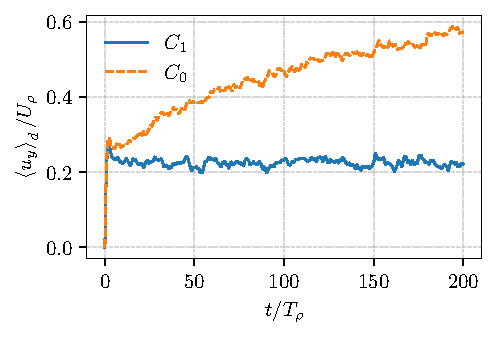
\includegraphics[height= 0.3\textwidth]{image/VALIDATION/C0C1/Ud.pdf}
    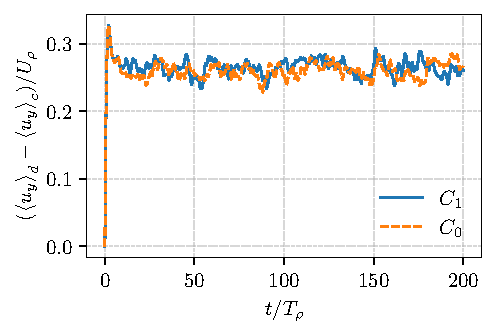
\includegraphics[height= 0.3\textwidth]{image/VALIDATION/C0C1/DeltaU.pdf}
    \caption{(left) Absolute averaged velocity of the dispersed phase along the vertical axis.
            (right) Relative velocity between the dispersed and continuous phases.
            (Dashed lines) simulation $C0$,
            (solid lines) simulation $C1$.  }
    \label{fig:VALIDATION_C0C1_1}
\end{figure}
On \ref{fig:VALIDATION_C0C1_1} we can observe the results of the two cases $C0$ and $C1$.
The (left) picture clearly shows that there is a velocity shift when no correction is applied.
Nevertheless, the two cases exhibit the same interphase velocity (see \ref{fig:VALIDATION_C0C1_1} (right)), which results in a same interphase drag force. 
The phase velocity is a term of first order, therefore it is no sensitive to the numerical parameters (e.g, number of drops per domain, number of cells per diameters).
Therefore, it is interesting to observe on \ref{fig:VALIDATION_C0C1_2}, that the similarities still holds on the first order closure terms. 
\begin{figure}[h!]
    \centering
    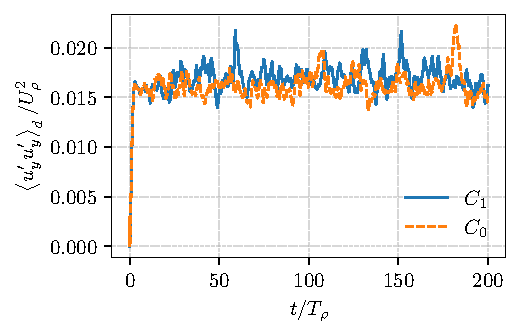
\includegraphics[height= 0.3\textwidth]{image/VALIDATION/C0C1/UpUpf.pdf}
    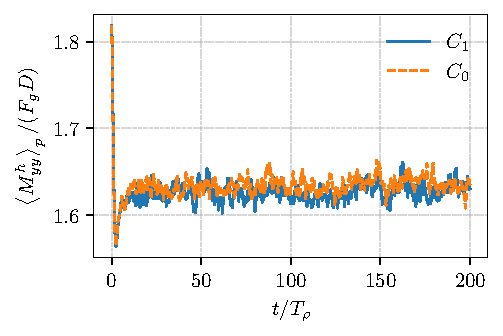
\includegraphics[height= 0.3\textwidth]{image/VALIDATION/C0C1/PA_Mh.pdf}
    \caption{(left) Fluids phase averaged fluctuation tensor.
            (right) Particular average of the first moment tensor, where $F_g$ is the buoyancy force applied on one droplet.
            (Dashed lines) simulation $C0$,
            (solid lines) simulation $C1$.  }
    \label{fig:VALIDATION_C0C1_2}
\end{figure}
Indeed, as we can remark the velocity fluctuations and the first moment are quite the same for both simulations.
It is not presented here, but all quantities remain the same thus the \textit{momentum corrector} isn't influencing any of these closures terms. 

\subsection{Number of particles per domain and definition of the mesh}

Now, let's investigate the required number of droplets per domain, $N_b$, and the minimum definition of cells per diameter of droplets $\delta$.  
\tb{Include bibliography and expectation here \ldots}
For this investigation we kept the physical parameters presented in the same section and made a double parametric analysis over $N$ and $\delta$. 
We carried out simulations for $N = 2, 3, 4, 5, 6, 7$, and for a number of cells $10 <\delta < 40$. 
In Basilisk the mesh definition is defined by a power of two, consequently depending on the size of the domain (which is fixed to keep a $\phi$ constant) the $\delta$ parameter is fixed at a power of 2 close. 
\begin{figure}[h!]
    \centering
    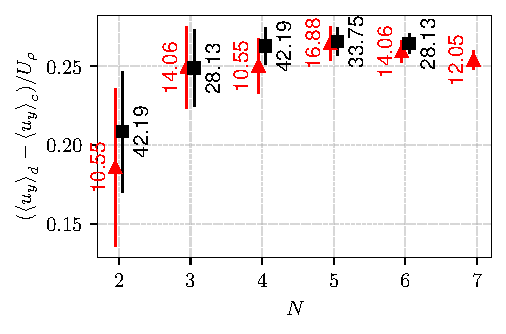
\includegraphics[height= 0.3\textwidth]{image/VALIDATION/N_and_delta/DUd.pdf}
    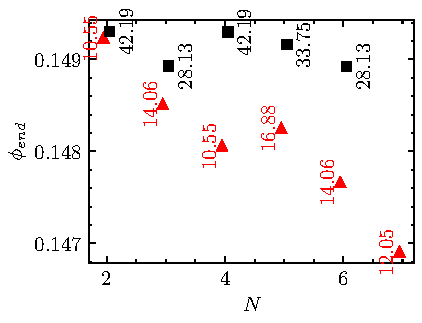
\includegraphics[height= 0.3\textwidth]{image/VALIDATION/N_and_delta/PHI.pdf}
    \caption{(left) Averaged relative velocities for both phases.
            (right) Dispersed phase volume fraction at the end of each simulation.
            The text on the side of the points is $\delta$. }
    \label{fig:VALIDATION_Nd_1}
\end{figure}
\ref{fig:VALIDATION_Nd_1}(left), illustrate clearly that the drift velocity is independent of the parameters $N_b$ and $\delta$, for $N >4$. 
On the other hand, \ref{fig:VALIDATION_Nd_1}(right), show that the volume fraction of the dispersed phase is lower for the low defined grid (red dots), due to a loss of volume during the simulation.
This doesn't mean that the solver isn't volume conservative. 
In fact, it is fund to be due to the \href{http://basilisk.fr/sandbox/fintzin/Rising-Suspension/no-coalescence.h}{no-coalescence.h} which generate fragment into the numerical domain, fragment which are deleted in the long run. 
\begin{figure}[h!]
    \centering
    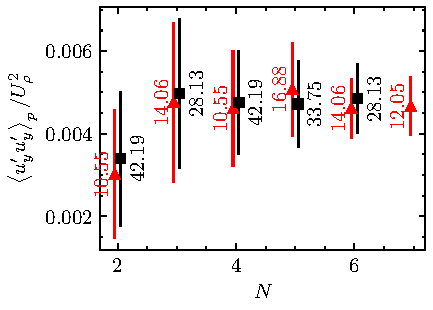
\includegraphics[height= 0.3\textwidth]{image/VALIDATION/N_and_delta/PA_UpUp.pdf}
    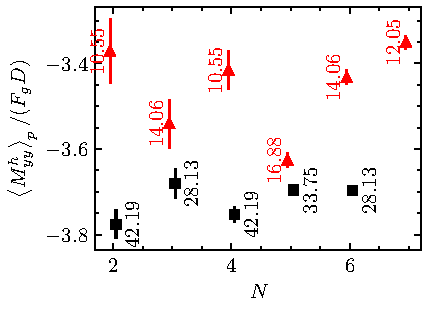
\includegraphics[height= 0.3\textwidth]{image/VALIDATION/N_and_delta/Mh.pdf}
    \caption{(left) Fluids phase averaged fluctuation tensor.
            (right) Particular average of the first moment tensor, where $F_g$ is the buoyancy force applied on one droplet. 
            The numerical values displayed alongside the dots are the number of cells per diameter.}
    \label{fig:VALIDATION_Nd_2}
\end{figure}
Now, let's look at the behavior of more \textit{complicated} closure terms. 
\ref{fig:VALIDATION_Nd_2}(left) demonstrate that the vertical component of the pseudo turbulent tensor is parameter independent rather early, independently of the grid definition. 
This fact is rather surprising but notice that the standard deviation is quite high for small domain. 
On \ref{fig:VALIDATION_Nd_2}(right), we can examine the vertical component of the first moment closure term. 
It is found to be constant for all $N$, but rather inaccurate for coarse grids. 
Which makes sens since the first moment results from a local calculation of the stress over a droplet volume, unlike the other quantities which results from the averaged center of mass velocity of a droplet. 

As we have shown, the quantities presented converge for a number of droplets equivalent to $N = 4$ and $\delta = 25$. 
Thus, we validate our simulation in space, i.e. we made sure that our domain were wide enough to minimize the influence of the periodicity on our results, and in mesh definition. 
Nevertheless, at it is the number of realization that matter when carrying a particular average, it is interesting to look at the duration of the simulation.

\subsection{Time average convergence}

The aim of this study is to be able to identify the minimum required time (or number of time steps) to obtain a representative mean. 
In this set of results we made sure that all the simulations were carried for a time that is more than sufficient. 
Therefore, in this section, we observe the convergence of the mean of a quantity depending on the number of the sample of time taken through the simulation.
More specifically we define the cumulative mean of an already, space averaged quantity, $F$, as, 
$\bar{F}(t) = \int_{T_{start}}^{t} F dt$. 
Where we introduced the start of sampling time $T_{start}$, which correspond to the starting time at which we are gathering data. 
This time is chosen as the time it takes for the simulation to reach a statistically steady state.
In other worlds, it is the time it takes for the droplets to get from an inert ordered state ($t = 0$), to a fully random state, where the droplets reach their mean drifting velocity.
As, we could remark, from its high standard deviation, the most difficult quantity, difficult in the meaning that it doesn't converge rapidly, is the \textit{Reynolds} stress tensor averaged on the particular phase, namely $\pnavg{u'_yu'_y}$.
Thus, we will confirm the representativity of our simulations, by looking at the cumulative time average of this quantity. 
\begin{figure}
    \centering
    % 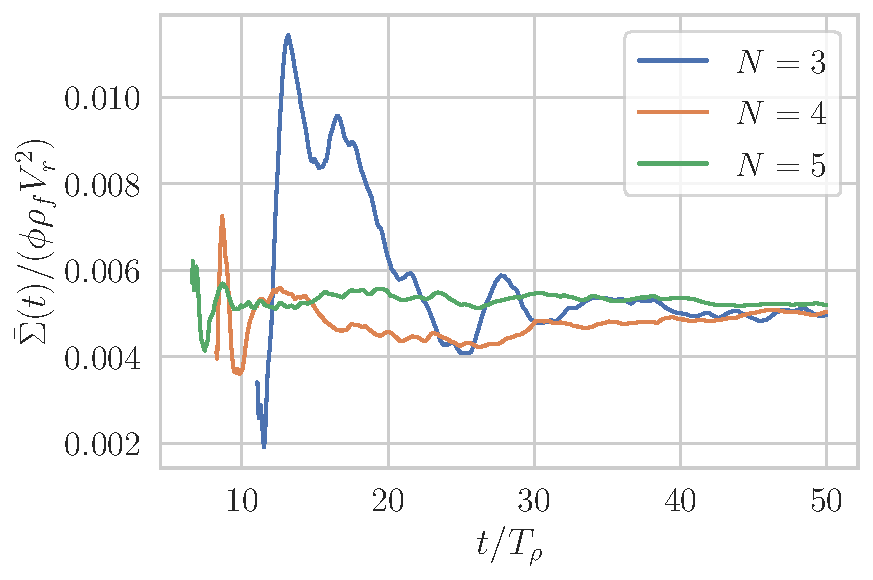
\includegraphics[height = 0.3 \textwidth]{image/VALIDATION/time/Sigma.pdf}
    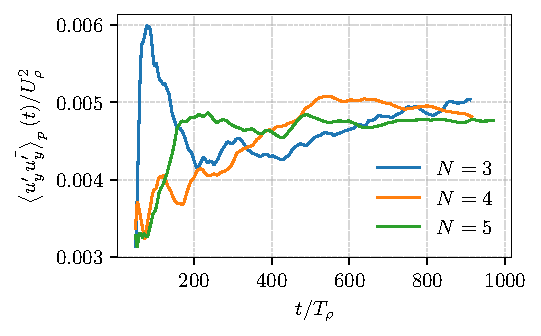
\includegraphics[height = 0.3 \textwidth]{image/VALIDATION/time/UpUp.pdf}
    \caption{Cumulative mean of the \textit{Reynolds} stress tensor. For $N = 3,4,5$ and $\delta = 25$, with $t/T_{start} = 10$.}
    \label{fig:VALIDATION_cumul_mean}
\end{figure}
From, \ref{fig:VALIDATION_cumul_mean}, it is apparent that the case where, $N=5$, has a faster convergent mean. 
Indeed, if we examine the picture, it is evident that the curve for $N=5$ reach a steady state earlier than the other ones. 
As a matter of fact, it can be perceived that the $N=5$ simulation reaches a steady mean at $t/T_\rho = 25$, while the other converge much latter. 
As a result, this study show, without surprise, that the result of the particular \textit{Reynolds} stress tends toward a steady mean faster for the simulation where $N=5$. 
In view of this it is interesting that for this range of \textit{Galileo} the time required to have significant results it $t/T_{\rho} \approx 110$, where we added the start time and $100$ inertial sampling time. 


\subsection{Asymptotic regime in low \textit{Galileo}}

Ideally we would like to cover a wide range of \textit{Galileo} numbers. 
Meaning that we need to reach both asymptotic regime, at low and high $Ga$ for any closure, if we suppose that such asymptotic regime exist. 
We limit our validation to the drag force or drift velocity closure term. 
In this section we show that in the limited range studied, i.e. $Ge \in [5,100]$, we cover enough \textit{Galileo} number to reach the low and high inertia asymptotic regime. 

First, it is interesting to see that the range of \textit{Galileo} number studied correspond to a wider range of \textit{Reynolds} numbers. 
Indeed, \ref{fig:Ga_Re} we clearly see that the computed \textit{Reynolds} numbers, based on the drift velocity, i.e. $Re = D (\cavg{\textbf{u}} - \davg{\textbf{u}}) \rho_f/\mu_f$, results in a wider range than the input \textit{Galileo} numbers. 
\begin{figure}[h!]
    \centering
    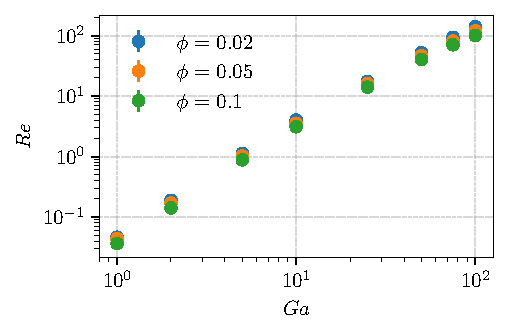
\includegraphics[height= 0.3\textwidth]{image/Dim_3/fCA/Re.pdf}
    \caption{\textit{Reynolds} number computed with the drift velocity, in terms of the \textit{Galileo} numbers.}
    \label{fig:Ga_Re}
\end{figure}
Thus, we cover both regime, inertial for $Re \approx 0.1$ and non-inertial with $Re \approx 100$. 
In order to investigate the different asymptotic regime of the drag force closure term, we plotted, in \ref{fig:f_u_f_rho}, the dimensionless drag force under two different form. 
In the first case (\ref{fig:f_u_f_rho}(left)) it is made dimensionless by the viscous material terms, namely,
\begin{equation*}
    \cavg{\textbf{f}^\mu} = \frac{\textbf{g} D^2\Delta \rho}{\mu_f |\cavg{\textbf{u}} - \davg{\textbf{u}}|}. 
\end{equation*} 
While in the other case it is made dimensionless with the inertial assumption, 
\begin{equation*}
    \cavg{\textbf{f}^\rho} = \frac{\textbf{g} D\Delta \rho}{\rho_f |\cavg{\textbf{u}} - \davg{\textbf{u}}|^2}. 
\end{equation*} 
\begin{figure}[h!]
    \centering
    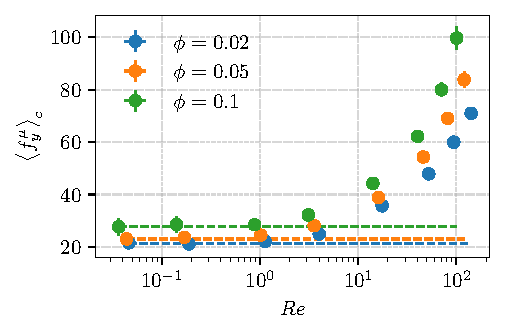
\includegraphics[height= 0.3\textwidth]{image/Dim_3/fCA/FH_Re_mu.pdf}
    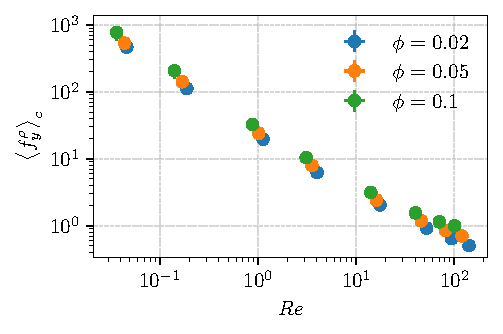
\includegraphics[height= 0.3\textwidth]{image/Dim_3/fCA/FH_rho_Re.pdf}
    \caption{(left) Non-inertial dimensionless vertical drag force term. 
             (right) Inertial dimensionless vertical drag force term. }
    \label{fig:f_u_f_rho}
\end{figure}
In \ref{fig:f_u_f_rho}(left) we can observe that $\cavg{\textbf{f}_\mu^*}$ tend to a constant value for approximately, $Re \le 1$, corresponding to a $Ga \le 5$.
Meaning, that we reach an asymptotic regime at $Ga=5$, and that it will probably tend to this same value at even lower $Re$ or $Ga$. 
However, as demonstrated by \ref{fig:f_u_f_rho} (right) the high inertial regime do not tend to a constant yet. 
Thus, no additional conclusion can be drawn so far for high inertial regime. 

In conclusion, in order to cover a wide enough range of \textit{Galileo}, we do not need to investigate $Ga<5$ since the lower \textit{Galileo} simulations, seems to behave proportionally to the case where $Ga = 5$. 
Regarding the high inertial regime, as we cannot really go above $Ga =100$ (due to the required mesh definition at higher $Ga$), we limit our study to $Ga =100$.  
Consequently, in the following simulation were carried though the range $Ga = [5,100]$, corresponding to $Re \in [1,100]$. 

\subsection{Statistical convergence}

\subsubsection{Pair PDF of presence}

In the next chapter we will see that the radial distribution function has a major importance in the closure problem. 
In order to be representative while reconstructing this function numerically, we need to gather enough sample of relative event of pairs of particles position. 
Thus, when $N$ increase, the number of particles realization of pairs of particles increase, thus we expect that $g(r)$ tends toward a constant function with increasing $N$. 
The question is, how many droplets per domain do we need so that this function is indeed representative (keeping the simulation time and time step constant) ? 
\begin{figure}[h!]
    \centering
    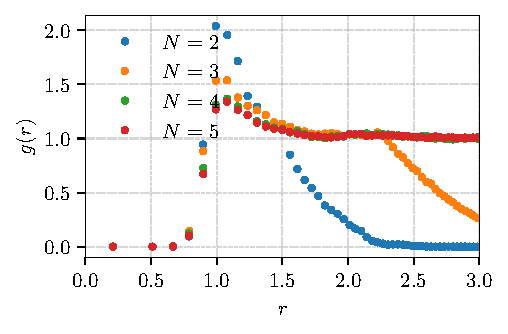
\includegraphics[height= 0.3\textwidth]{image/VALIDATION/fDist/g_r.pdf}
    \includegraphics[height= 0.3\textwidth]{image/VALIDATION/fDist/N_g_1.pdf}
    \caption{(left) Plot of the radial distribution function $g(r)$ for different $N$. 
             (right) Plot of the values of $g$ for $r =1$ in terms of the number of droplets inside the domain for different mesh definition. }
    \label{fig:g_r}
\end{figure}
On \ref{fig:g_r} (left), we see that the radial distribution function $g(r)$, tends to one with increasing $r$, which is exactly what we expect from a radial distribution function, thus it is a first validation. 
Moreover, the value of the radial distribution at $r\approx1$, is of a major importance since it is used in a closure models for the particular phase averaged stress in solid particle suspensions \citep{jackson2000dynamics}, it is also used in kinetic theory for the collision kernel modeling, \citep{fede2015monte}.
Therefore, \ref{fig:g_r} (right) we plotted the value of $g(r=1)$ for different mesh definition and number of particles per domain. 
It is evident that $g(1)$ reach a constant value above $N=4$ for a mesh definition $\delta = 25$. 

We established that the statistical distribution converged radially. 
Nevertheless, we would like to study the angular distribution in addition to the radial distribution.  
Thus, on \ref{fig:VALIDATION_fDrop_3} we show different 2D plots of this 2D distribution function. 
By comparing both plot it clearly indicates that this 2 dimensional distribution converge at $N=5$. 
\begin{figure}[h!]
    \centering
    % 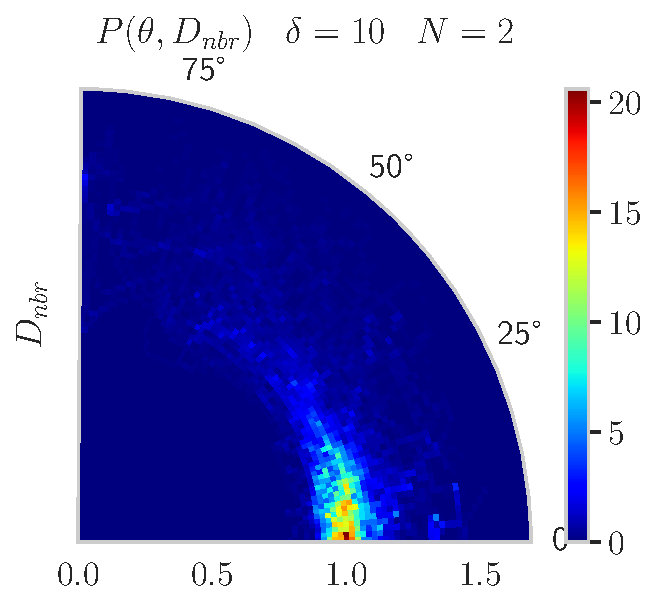
\includegraphics[height= 0.35\textwidth]{image/VALIDATION/fDrop/D_nbr_Theta_ndc_10_N_2.pdf}
    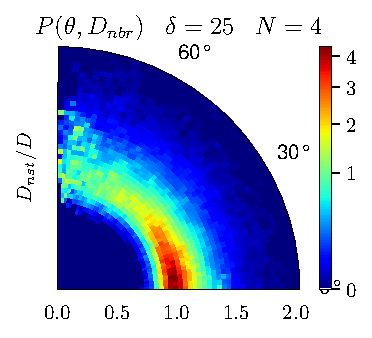
\includegraphics[height= 0.3\textwidth]{image/VALIDATION/fDrop/U_Theta_ndc_25_N_4.pdf}
    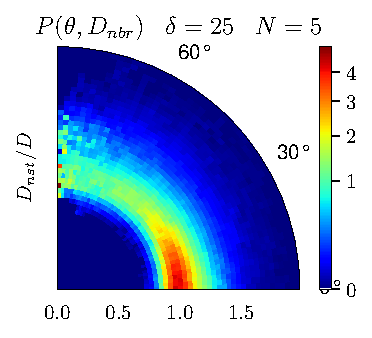
\includegraphics[height= 0.3\textwidth]{image/VALIDATION/fDrop/U_Theta_ndc_25_N_5.pdf}
    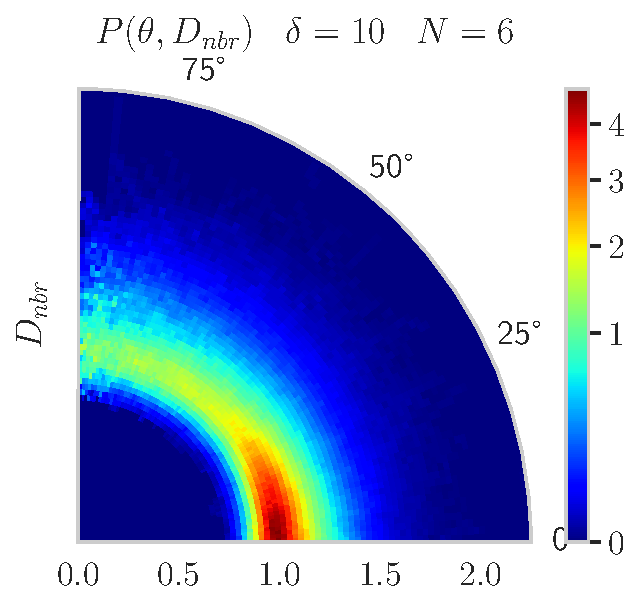
\includegraphics[height= 0.3\textwidth]{image/VALIDATION/fDrop/U_Theta_ndc_10_N_6.pdf}
    % 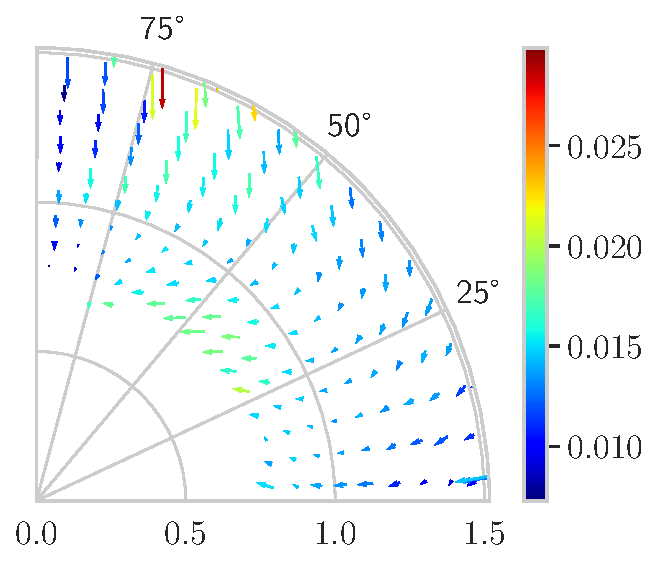
\includegraphics[height= 0.35\textwidth]{image/VALIDATION/fDrop/Dmin_Theta_Ur_uT_75_PHI_0_15.pdf}
    \caption{Radial distribution function of the nearest particle, $P(\theta, D_{nst}/D)$. 
    From $N=4$ (left) to $N=6$ simulations (right).}
    \label{fig:VALIDATION_fDrop_3}
\end{figure}
Indeed, if we look to the color bar of each plot and to the plot itself, we clearly see that the value of the PDF is the same for all $N$. 
Nevertheless, we can distinguish a small difference between $N=4$ and the others, even though it is small it deserves to be notified. 
Therefore, we consider a 2D distribution independence above a number of 64 ($N=4$) droplets per domain. 


\subsubsection{Influence of the mesh definition on nearest statistics}

Now that the required number of sample is fixed need to check out the influence of the mesh definition at the inter particle scale. 

To do so we propose to study the following a case with the following dimensionless numbers. 
We set $Ga = 75$ to be in the most disadvantageous situation. 
\begin{align}
    Ga = 75
    & \phi = 0.1
    & \mu_r =0.1 
    & \rho_r = 1.1
    & Bo = 1 
\end{align}
Finlay we test three number of cells quality, $\delta > 10$, $\delta > 25$, $\delta > 35$. 


\section{Experimental design}

From the previous few sections, we were able to identify and select relevant dimensionless parameters 
to be studied in the next chapters. 
They were deduced from parameters independence depicted in the previous few sections.
They are summaries in \ref{tab:parameters2}.
\begin{table}
    \caption{Ranges of the studied dimensionless parameters.}
    \centering
    \begin{tabular}{|c|c|c|c|c|c|c|} \hline
        $Ga$ &
        $\phi$ & 
        $Bo$ &
        $\rho_r$ &
        $\mu_r$ &
        $T_{max}/T_g$ &
        $\Delta t/T_{\sigma}$\\ \hline
        5-100
        &0.01-0.15
        & 1 
        & 1.1
        & 0.1-10
        & 500
        & 10 \\\hline
    \end{tabular}
    \label{tab:parameters2}
\end{table}
Most of the parameters have been discussed above. 
Regarding, $\phi$ we limited our study below $0.15$ because above this value bubbles or droplets instantaneously coalesce and the flow isn't dispersed anymore. 
Below $\phi =0.01$ the required domain is too wide, thus the simulations would be too expensive to carry, even though lower volume fraction would have been of interest. 
The \textit{Bond} number has been determined based on the shape of the particles. 
Indeed, we know that for extremely low $Bo$ a droplet will remain spherical. 
Thus, as for our application (see introduction of \ref{chap:avg}) we aim for spherical droplets, i.e. \textit{Bond} numbers, we need to seek for convergence toward low $Bo$. 
And as it will be shown in the results, for $Bo =1$, and this range of $Ga$, the particles remain spherical, thus we reach this asymptotic regime for low $Bo$. 
The density ratio $\rho_r = 1.1$ correspond to the ratio of our application. 
Regarding, the viscosity ratio our application (oil /water) is at $\mu_r=0.1$, but we allow our selves to explore a wider range event though we won't be able to describe entirely this dimension. 
The time of the simulation is scaled on the inertial time, $T_\rho$, as the simulations are mostly driven by inertial effect (i.e. $Ga \in [5,100]$). 
The value of $500$ inertial time has been validated empirically as can be shown by the accuracy of the previous results. 
The time step has been scaled with the capillary time in order to sample several time steps in a period of deformation of a droplet. 

In brief, the numerical parameters together with the physical ones are well validated.
Therefore, in the following chapters we carry out simulations in the restricted ranges of the parameters depicted \ref{tab:parameters2}.



\chapter{Mono-disperse buoyant water/oil emulsion.}
\label{chap:mono-disperse}

In this chapter we present the results related to the mono-disperse buoyant rising  emulsion of droplets.
All the simulations files can be found here \url{http://basilisk.fr/sandbox/fintzin/Rising-Suspenion/}
This chapter will cover the different closure terms that we brought to light in \ref{chap:avg}, such as the mean slip velocities or drag force, the Reynolds stress tensor and the particle stress tensor.
Even through we forced non coalesce in these simulations we will still discuss the possibility to close the collision kernel of PBE or Lagrangian equations. 
Also in this chapter we will solely focus on the momentum equations closure, and neglect mass transfer terms. 
\begin{figure*}
    \centering
    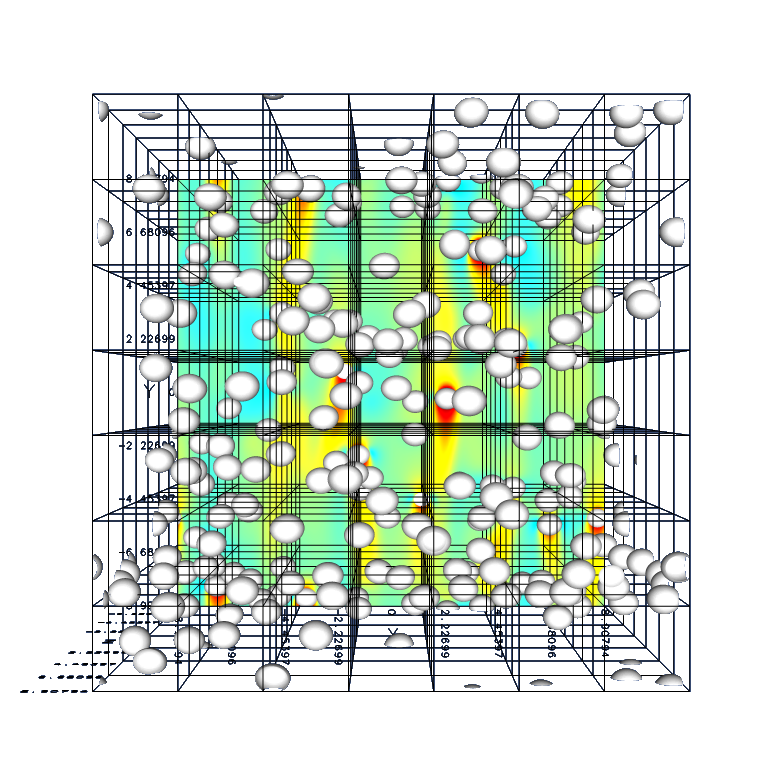
\includegraphics[width = 0.8 \textwidth]{image/PHI_01_Ga_75.png}
    \caption{Snapshot of a simulation at $T_g = 300$ for $\phi = 0.1$, $Ga = 75$ $\mu_r = 0.1$ and $N_b = 125$. In white : the interfaces, The background color map correspond to the pressure field. The grid represents the different core.}
    \label{fig:pic_sim}
\end{figure*}
As a consequence of the mono-disperse assumption it is evident that the mass balance and number density balance are similar. 
However, the surface balance (\ref{eq:A_avg_p}) remains relevant as the surface of all particles is not constant since it is a function of the deformation. 
However, as it will be shown in the low \textit{Bond} numbers limit the droplets remain spherical allowing us o discard this equation too. 
Therefore, In this context we be interested in the momentum balance's (\ref{eq:classic_hybrid_momentum_p} and \ref{eq:classic_hybrid_momentum_c}) closures. 
Neglecting the mass transfer terms and considering the mass as a constant yields the following particular and continuous averaged momentum equations, 
\begin{multline}
    \rho_c\pddt (\phi_c\cavg{\textbf{u}}) 
    + \rho_c\nablab \cdot ( \phi_c \cavg{\textbf{u}}\cavg{\textbf{u}})
    = \pavg{\int_{S_\alpha} \textbf{T}_c  \cdot \textbf{n}_c d S}
    +\phi_c\cavg{\textbf{b}}\\
    + \nablab\cdot\left[
    \phi_c \cavg{\textbf{T}}
    - \pavg{\int_{S_\alpha} \textbf{r} \textbf{T}_c  \cdot \textbf{n}_c dS}
    - \rho \cavg{\textbf{u}'\textbf{u}'}
    \right],
    \label{eq:homo_momentum_c}
\end{multline}
\begin{multline}
    \pddt   \left(\pavg{\textbf{u}_\alpha}\right)
    + \nablab \cdot \left(\pavg{\textbf{u}_\alpha}\pnavg{\textbf{u}_\alpha}\right)
    = \frac{n}{m_\alpha}\pnavg{\int_{V_\alpha} \textbf{b} dV}\\
    + \frac{n}{m_\alpha}\pnavg{\int_{S_\alpha} \textbf{T}_c  \cdot \textbf{n}_c dS}
    - \nablab \cdot \left(\pavg{\textbf{u}_\alpha' \textbf{u}_\alpha'}\right). 
    \label{eq:homo_momentum_p}
\end{multline}
From these simplified equations we can start to complete the closure problem.

Since all simulations reach as quasi static regime we can stipulate that the averaged velocities vector are constants and vertical. 
Therefore, all along this chapter we note the drift velocity such as $U = \pnavg{\textbf{u}} - \cavg{\textbf{u}}$. 
Besides, in this chapter we fix the following dimensionless parameters to $\rho_r =1.11 $, $\mu_r =0.1$, $Bo =1$ and $N_b = 125$. 
As a consequence of the small \textit{Bond} number in presence, the droplets are nearly spherical. 
A picture of a typical simulation is shown \ref{fig:pic_sim}
\section{The drag force term}
We start by the drag force term. 
Our simulations reach a quasi steady regime meaning that we can consider the velocities of the particular phase and fluid phase as constant.
Now lat's place our selves in the reference frame moving at the averaged velocity of the particles. 
In this frame of reference the particles are thus fixed and see the fluid flowing through, experiencing a drag force due to the stress on the droplets surface. 
Therefore, in this referential considering $\pavg{\textbf{u}} = \textbf{0}$, the momentum equation \ref{eq:homo_momentum_p} yields, 
\begin{equation*}
    m_\alpha \grad \cdot \left(\pavg{\textbf{u}_\alpha' \textbf{u}_\alpha'}\right). 
    = \pavg{\int_{V_\alpha} \textbf{b} dS}
    + \pavg{\int_{S_\alpha} \textbf{T}_c  \cdot \textbf{n}_c dS}
\end{equation*}
\tb{to be disscused}
We can observe that the divergence of the fluctuation is balanced by the two contributions to the RHS.  
Besides, the body force term has the simple expression, $\pavg{\int_{V_\alpha} \textbf{b} dV} = - nV_\alpha (\rho_d-\rho_c) \textbf{g}$. 
Therefore, the drag force term must be expressed as the sum of a pure drag force which balance the body force and a divergence of a stress which balance in this can the Reynolds stress \citep{zhang2021ensemble,wang2021numerical,nott2011suspension}. 
In this section we focus on the pure drag component and expresses it in the dimensionless form such as, 
\begin{align*}
    \pnavg{F_\mu}
    = \frac
    {\pnavg{\int_{V_\alpha} \textbf{T}\cdot \textbf{n}dV}}
    {\mu_c U D}
    = \frac
    {\left(\rho_d -\rho_c\right) \textbf{g}}
    {\mu_c U}D^2
\end{align*}
Where $\pnavg{F_\mu}$ is the pure dimensionless drag force along the direction of the velocity. 

\ref{fig:f_mu} displays the interphase drag force for different \textit{Galileo} number and volume fraction. 
\begin{figure}[h!]
    \centering
    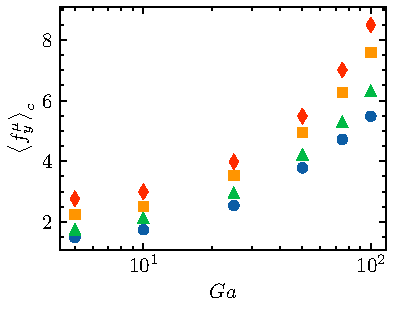
\includegraphics[height=0.3\textwidth]{image/HOMOGENEOUS/fCA/FH_mu_Ga.pdf}
    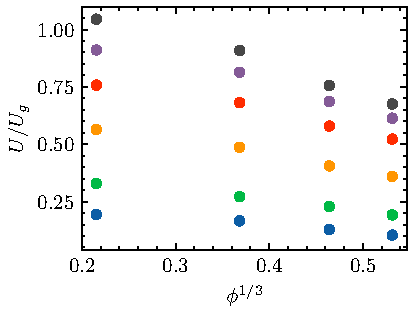
\includegraphics[height=0.3\textwidth]{image/HOMOGENEOUS/fCA/UstokesGa.pdf}
    \caption{(left) Dimensionless drag forces in terms of the \textit{Galileo} number for different volume fraction $\phi$. The other parameters are fixed at $\rho_r = 1.11$, $\mu_r = 0.1$ and $Bo = 1$.
    (dots) Numerical simulations, 
    (dashed line) empirical formula \ref{eq:f_mu_scaling}.
    (right) Dimensionless drift velocity.}
    \label{fig:f_mu}
\end{figure}
Based on the numerical results we could find simple scaling for the drag force at moderate inertial regime. 
Indeed, it yields,
\begin{equation}
    \cavg{F^\mu} = e^{5.66 \phi^{1/3}}  Ga^{0.33} 0.59 + Ga^{0.92} +18.29
    \label{eq:f_mu_scaling}
\end{equation}
From \ref{fig:f_mu} and \ref{eq:f_mu_scaling} it is evident  that in low inertial regime, the drag force scales as $f \sim Ga^{0.33}$ regardless of the volume fraction. 
Regarding the dependency of the force with $\phi$, we observe that the logarithms of the force is proportional $\phi^{1/3}$. 
This reminds the scaling of \cite{sangani1987sedimentation} which found the same $\phi$'s dependency, but on the drift velocity of arranged bubbles arrays.
This scaling is illustrated \ref{fig:f_mu} (right) where we can see that the drift velocity is indeed proportional to $\phi^{1/3}$ regardless of the \textit{Galileo} number.  
\section{Reynolds stress closure}
Now let's investigate the Reynolds stress sensor, for both the continuous and the particular phase.
We first decompose the stress tensor by a sum of a spherical and deviatoric part \citep[chapter 6]{morel2015mathematical}, such as, 
\begin{equation*}
    \cavg{\textbf{u'u'}}
    = \frac{2}{3}\cavg{T}\left(
        \textbf{I}
        + \cavg{\textbf{B}}
    \right),
\end{equation*}
where we introduced the turbulent kinetic energy, $\cavg{T} = \frac{1}{2}\cavg{\textbf{u'u'}}:\textbf{I}$ and the deviatoric part of the Reynolds stress as, 
$\cavg{\textbf{B}} = \cavg{\textbf{u'u'}}/(2\cavg{T}) - \frac{1}{3}$.
A similar logic can be applied to the particular averaged Reynolds stress yielding, 
$
\pnavg{\textbf{u}'_\alpha \textbf{u}_\alpha'}
    = \frac{2}{3}\pnavg{T_\alpha}\left(
        \textbf{I}
        + \pnavg{\textbf{B}_\alpha}
    \right)
$.
In this case $\pnavg{T_\alpha}$ is the granular temperature from kinetic theory \citep{rao2008introduction}. 
Note that the non-diagonal components of $\cavg{\textbf{B}}$ and  $\pnavg{\textbf{B}_\alpha}$ are all null due to the symmetry of the model. 
Therefore, they will not be shown here. 
\subsection{The continuous phase Reynolds stress}
The fluid averaged kinetic energy can be easily scaled on the numerical results shown \ref{fig:Tf_Bf}(left).
Indeed, we found out that 
\begin{equation}
    \frac{\cavg{T}}{U^2} \approx \frac{\phi}{Ga^2}5.98\cdot10^{4} ,
    \label{eq:Tf_scaling}
\end{equation}
where we use the drift velocity $U$ to make $T$ dimensionless. 
\begin{figure}[h!]
    \centering
    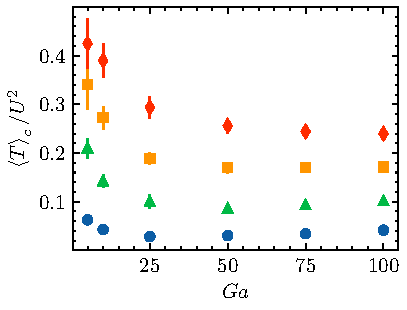
\includegraphics[height=0.3\textwidth]{image/HOMOGENEOUS/fCA/Tf.pdf}
    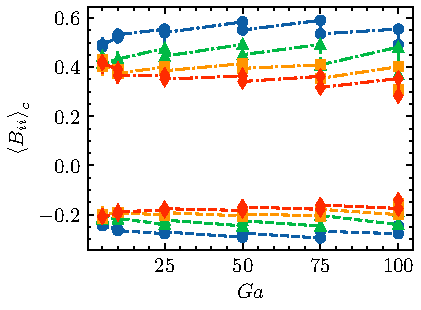
\includegraphics[height=0.3\textwidth]{image/HOMOGENEOUS/fCA/Bf.pdf}
    \caption{(left) Dimensionless turbulent kinetic energy in terms of the \textit{Galileo} number for different $\phi$. (dots) Numerical simulations, (dashed line) empirical formula \ref{eq:Tf_scaling}.
    (right) deviatoric part of the Reynolds stress, ($\bullet$) are the vertical components, $B_{yy}$, ($\blacktriangle$) are the horizontal components, $B_{xx} = B_{zz}$.}
    \label{fig:Tf_Bf}
\end{figure}
In opposition to the drift velocity, the dimensionless turbulent kinetic energy scale as $\sim \phi$ regardless of the \textit{Galileo} number. 
As shown previously $U \sim \phi^{1/3}$, consequently the turbulent kinetic energy scale as $\cavg{T} \sim \phi^{5/3}$. 
Besides, $\cavg{T}$ is a monotonic function of $Ga$ with a growth rate of $0.91$. 
Regarding the deviatoric part of the Reynolds stress tensor, namely, $\cavg{\textbf{B}}$, it can be approximated by, roughly, $\cavg{\textbf{B}_{yy}} \approx 0.4$ and $\cavg{\textbf{B}_{zz}} = \cavg{\textbf{B}_{xx}}  \approx - 0.2$.
Therefore, the \textit{Reynolds} stress is clearly oriented, indeed the stress is greater in the direction of the flow. 
Also, as depicted by \ref{fig:Tf_Bf} (right), at high $Ga$ and $\phi$ those components slightly tend to lower values, whether it is for the horizontal or vertical components. 
This means that the global Reynolds stress tends to be isotropic with for high $Ga$ and $\phi$. 
In \citet{jackson2000dynamics} they stipulate that at high rate of collision the \textit{Reynolds} stress tends to be isotropic. 
Which is in accordance with our findings since, $Ga$ and $\phi$ are directly correlated to the rate of collision. 
For now a good approximation of $\cavg{\textbf{B}}$ is 
\begin{equation}
    \cavg{\textbf{B}} 
    \approx 0.4 \textbf{dd} + 0.2 (\textbf{I} - \textbf{dd}),
    \label{eq:Bf_scaling}
\end{equation}
where $\textbf{d}$ is the unit vector following the direction of the flow, in our case, $\textbf{d} = \textbf{g}/g$ or more generally, $\textbf{d} = U/|U|$. 

\subsection{The particular phase Reynolds stress}
Now let's focus on the particular averaged Reynolds stress tensor.
\ref{fig:Talpha_Balpha} shows that the granular temperature behavior is quite similar from the continuous averaged turbulent kinetic energy.
\begin{figure}[h!]
    \centering
    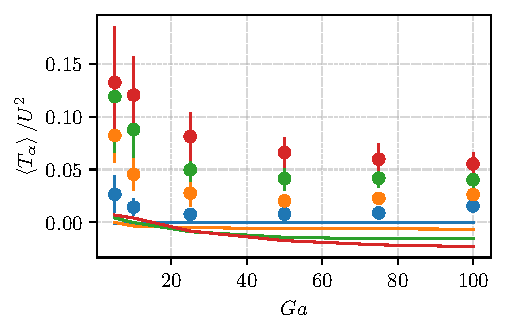
\includegraphics[height=0.3\textwidth]{image/HOMOGENEOUS/fPA/Talpha.pdf}
    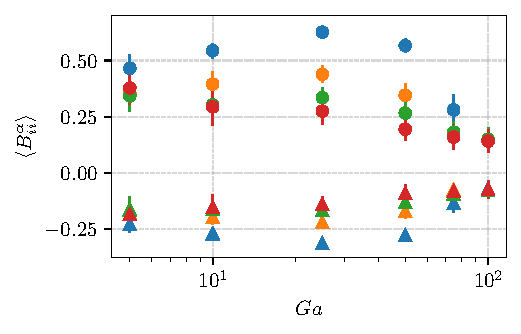
\includegraphics[height=0.3\textwidth]{image/HOMOGENEOUS/fPA/Bf.pdf}
    \caption{(left) Dimensionless turbulent kinetic energy in terms of the \textit{Galileo} number for different $\phi$. (dots) Numerical simulations, (dashed line) empirical formula \ref{eq:Talpha_scaling}.
    (right) deviatoric part of the Reynolds stress, ($\bullet$) are the vertical components, $B_{yy}$, ($\blacktriangle$) are the horizontal components, $B_{xx} = B_{zz}$.}
    \label{fig:Talpha_Balpha}
\end{figure}
We can also provide a scaling for the granular temperature, it reads as,  
\begin{equation}
    \frac{\pnavg{T_\alpha}}{U^2}  \approx \frac{\phi}{Ga^2} 2.86\cdot10^{4} 
    \label{eq:Talpha_scaling}
\end{equation}
From \ref{fig:Talpha_Balpha} we observe that this scaling is valid for the lowest \textit{Galileo}. 
The deviatoric part of $\pnavg{T_\alpha}$ is displayed on \ref{fig:Talpha_Balpha}.
It tells us that the Reynolds stress for the particular phase tends to be isotropic in the same way as $\cavg{T}$. 
Indeed, the components of $\pnavg{\textbf{B}}$ go to zero with increasing $Ga$ and $\phi$. 
This behavior is explained by the higher rate of collision present for higher volume fraction and inertia \citep[chapter 1]{jackson2000dynamics}
\section{The first moment}
In this section we will be interested into the first moment tensor appearing in \ref{eq:homo_momentum_c}, namely the average of the tensor $\textbf{D}_\alpha = \int_{S_\alpha} \textbf{r}\textbf{T}_c\cdot \textbf{n}_c dS = \int_{S_\alpha} \textbf{rf}_c dS$, where we introduced the microscopic hydrodynamical force vector $\textbf{f}_c = \textbf{T}_c\cdot \textbf{n}_c$.
Following the same approach as the analysis of \citet[chapter 2]{kim2013microhydrodynamics} we decompose the first moment tensor into two distinct tensors and remove the isotropic part of $\textbf{D}_\alpha$, yieldings
\begin{equation*}
    \textbf{D}_\alpha - \frac{1}{3}(\textbf{I}:\textbf{D}_\alpha)\textbf{I}
    = \textbf{S}_\alpha+\textbf{T}_\alpha,
\end{equation*}
where $\textbf{S}_\alpha$ is the stresslet tensor and $\textbf{T}_\alpha$ the hydrodynamical torque acting on the particle. 
Besides, because of numerical limitations, we prefer to use the force defined inside the dispersed phase $\textbf{f}_d$ instead of original force, $\textbf{f}_c$. 
It is possible to switch from a force to another by making use of the jumps condition (\ref{eq:stressjump}) defined in \ref{chap:avg}, i.e. $\textbf{f}_c = \textbf{f}_I - \textbf{f}_d$. 
Consequently, we can write that $\textbf{D}_\alpha = \textbf{D}_\alpha^I + \textbf{D}_\alpha^h$, where $\textbf{D}_\alpha^h$ is the hydrodynamical contribution to the first moment and $\textbf{D}_\alpha^I$ the surface tension force contribution. 
Applying the same decomposition for the torque and stresslet tensors yields,
\begin{align*}
    \textbf{S}_\alpha^h &= 
    \frac{1}{2}\int_{S_\alpha}
    \left(
        \textbf{r} \textbf{f}_d + \textbf{f}_d \textbf{r}
    \right)dS
    - \frac{1}{3}\int_{S_\alpha}
        (\textbf{r} \cdot \textbf{f}_d )\textbf{I}
        dS,\\
        \textbf{T}_\alpha^h &= 
    \frac{1}{2}\int_{S_\alpha}
    \left(
        \textbf{r} \textbf{f}_d - \textbf{f}_d \textbf{r}
    \right)dS,
\end{align*}
where we defined $\textbf{S}_\alpha^I$ and $\textbf{T}_\alpha^I$ as the contribution of the surface tension force and $\textbf{S}_\alpha^h$ and $\textbf{T}_\alpha^h$ as the hydrodynamical contribution.

The surface tension part of the first moment, $\pnavg{\textbf{D}_\alpha^I}$, can be obtained theoretically. 
Indeed, in the limit of low \textit{Bond} numbers the droplets are in average spherical.
Therefore, it is possible to compute the integral, $\int_{S_\alpha} \textbf{r} \textbf{f}_I dS$, analytically since $\textbf{f}_I $ is solely a function of the shape.
Then, the first moment of the surface tension force turns out to have the simple expression, 
\begin{align*}
    &\pnavg{\textbf{D}_\alpha^I}
    = \frac{2V_\alpha\sigma}{D_\alpha}  \textbf{I}
    &
    \text{and} 
    &&
    \pnavg{\textbf{S}_\alpha^I}
    =\pnavg{\textbf{T}_\alpha^I}
    = 0&
\end{align*}
For a detailed derivation we refer the reader to \ref{ap:cinematic}. 
It is also possible to consider other shapes than spherical, such as oblate and spheroid particles. 
These shapes might be considered for high $Bo$ and $Ga$ flows, since the droplets' shape can be approximated as a spheroid.
Again, we encourage the reader to look at \ref{ap:cinematic} for a detailed derivation of $\textbf{D}_\alpha^I$.  

Regarding the first moment generated by hydrodynamic forces theoretical investigation are not in order for the range of parameters studied here, therefore we expose our numerical results. 
First, notice that due to the symmetry of the numerical simulations all the non-diagonal components of $\textbf{D}_\alpha$ are null.
Consequently, the only non-null components in homogeneous rising suspensions flows are the three diagonal components of $\textbf{S}_\alpha^h$.
\begin{figure}[h!]
    \centering
    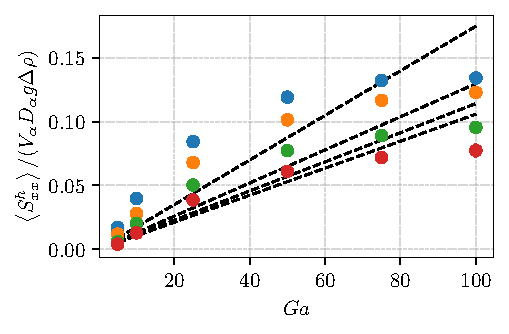
\includegraphics[height=0.3\textwidth]{image/HOMOGENEOUS/fPA/Sxx.pdf}
    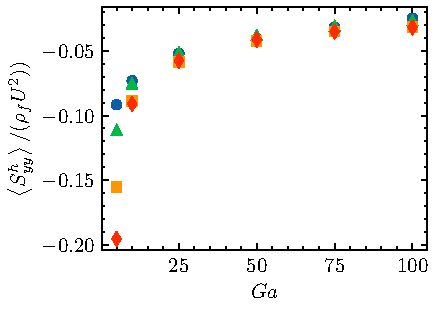
\includegraphics[height=0.3\textwidth]{image/HOMOGENEOUS/fPA/Syy.pdf}
    \caption{(left) Dimensionless trace of the first moment in terms of the \textit{Galileo} number for different $\phi$. (dots) Numerical simulations, (dashed line) empirical formula \ref{eq:trD_scaling}.
    (right) Dimensionless diagonal components of the stresslet tensor, ($\bullet$) are the vertical components, $S^\alpha_{yy}$, ($\blacktriangle$) are the horizontal components, $S^\alpha_{xx} = S^\alpha_{zz}$. (dashed line) empirical formula \ref{eq:B_scaling}.}
    \label{fig:trD_Sx_Sy}
\end{figure}
On \ref{fig:trD_Sx_Sy} we can observe that the dimensionless first moment's trace or spherical part has a quite simple tendency with the Galileo number.
Indeed, as depicted by the black dashed line in \ref{fig:trD_Sx_Sy} (left) the first moment behave in the dilute limit as a linear function with the \textit{Galileo} number, 
\begin{equation}
    \frac
    {\pnavg{\textbf{I}:\textbf{D}_\alpha^h}}
    {3V_\alpha D_\alpha g (\rho_f - \rho_d)}
    \sim  -1.44\cdot 10^{-03} Ga.
    \label{eq:trD_scaling}
\end{equation}
However, it possesses a non-monotonic behavior with respect to $\phi$. 
Determining whether the observed effect is a result of a numerical artifact or due to physical phenomenon is difficult to figure out.

On \ref{fig:trD_Sx_Sy} (right) we observe the proportion of each component of $\textbf{S}_\alpha^h$. 
Thus, we remark that the first moment gets isotropic for low $Ga$ and high $\phi$.
Then, the first moment decrease in the direction of the flow and increase on the direction perpendicular to the flow, as indicated by the ratios on the \ref{fig:trD_Sx_Sy} (right).
In conclusion, we suggest the following empirical formula for the first moment valid in the dilute regime, namely
\begin{equation}
    \pnavg{\textbf{S}^h_\alpha}
    =\frac{1}{3} \pnavg{\textbf{I}:\textbf{D}_\alpha}
    \left(
        \textbf{I} 
        + \pnavg{\textbf{B}}
    \right),
\end{equation}
where $\pnavg{\textbf{I}:\textbf{D}_\alpha}$ is defined by \ref{eq:trD_scaling} and $\pnavg{\textbf{B}}$, by,
\begin{equation}
    \pnavg{\textbf{B}} = 3.93 \cdot 10^{-04} ((\textbf{I}-\textbf{dd})-2\textbf{dd}).
    \label{eq:B_scaling}
\end{equation}
Based on this last empirical formula we observe that the stresslet is twice larger and with opposite sign in the direction of the flow than on the plan normal to the flow direction. 
In other words the mean force traction on the surface of the particle is in traction in the direction of the flow and in compression in the plan normal to the flow, besides the force traction is twice larger in the direction of the flow. 
\section{Statistical closure}

Consider doing machine learning to predict the collision normal velocity used in coalescence model

This way you can predict knowing the angle of attack the relative velocity or foces. 

INPUT, pos angle and Ga Phi. 
input learned through statisticla arguments. 

OUT, Rel vel and forces. 






%cll

The original issue addressed in this work is to find an appropriate method to represent emulsion or any ploy disperse multiphase flow within an averaging framework.
Indeed, due to the multiscale physical phenomenon present in those flows it is rather difficult to model the classical governing equations of fluids mechanics.  
Therefore, in this manuscript we presented a clear workflow providing accurate tools for the modeling of multiphase flows. 

The devellopement presented in this manuscript can be summaries into 9 key points:
\begin{enumerate}
    \item \ref{chap:daniel1} provides a derivation of the averaged equations governing the motion of dispersed two-phase flows with interfacial transport. 
    The averaged equations for the dispersed phase are derived through two distinct approaches: the particle-averaged (or Lagrangian) formalism, and the phase-averaged method. 
    The main conclusion of this work is the demonstration of the relation between the particle-averaged and phase-averaged equations. 
    We show that the dispersed phase-averaged equations can be interpreted as a series expansion of the particle-averaged moment equations. 
    The paper concludes by presenting a "hybrid" set of equations, consisting of phase-averaged equations for the continuous fluid phase, complemented by an arbitrary number of moment conservation equations for the dispersed phase.
    \item Following this we expose in \ref{chap:daniel15} the mass, momentum and energy averaged equations, using the ``hybrid'' formalism, that are necessary to describe buoyant emulsions. 
    Notably, this derivation allowed us to discuss the energy exchange present in an emulsion.
    Additionally, we provided an explicit and general formulation for the effective stress of an emulsion.
    \item \ref{chap:deformable} we consider spheroidal droplets geometry and show how from the first moment of momentum and second moment of mass equation we could derive tensor equations for the particle mean shear rate and deformation tensor. 
    This leads to a set of equation which closely reassemble the second-order forced oscillatory model, which describe the droplets' deformation. 
    With our formalism, we were able to express explicitly, in terms of local instantaneous properties of the flows, what are the forcing terms of this equation.  
    \item In \ref{chap:daniel2} we demonstrate how to reformulate any ensemble averaged terms into what we call \textit{single-particle conditional} averaged quantities. 
    Doing so, we propose a better formulation for partitioning the total momentum exchange term, showing that the usual formulation originally proposed by \citep{zhang1997momentum} might lead to inconsistent formulations. 
    On another hand we revisit the derivation of (2.10) of \citet{batchelor1972sedimentation} which relates continuous phase ensemble-averaged quantities to single-particle conditionally averaged quantities.
    Notably, we show that the assumptions made by \citet{batchelor1972sedimentation} to derive its formula are not sufficient to arrive at the actual expression given by (2.10), which explains the non-converging issue sometimes encountered using this formula. 
    To obtain the conditional averaged quantities, we follow \citet{hinch1977averaged}, and we propose a generic routine to derive the \textit{single-particle conditional averaged} Navier-Stokes equations. 
    We show that in the limiting case of low volume fraction, we find back the classic equations of the disturbance fields of an isolated particle immersed in an unbounded fluid. 
    Additionally, we demonstrate that our method can be extended to more complicated situations, which might lead to the consideration of inertia, non-vanishing volume fraction of particles, or gradient of concentration for example.
    \item In \ref{chap:daniel2}, we re-derived most of the closures present in the hybrid model. 
    While many of these were already established \citep[Appendix A]{zhang1997momentum}, we introduced several new closures, specifically: 
    The pseudo-turbulent stress $\avg{\chi_f \textbf{u}_f'\textbf{u}_f'}$ generated by a mean shear flow $\textbf{E}_f$ on droplets; 
    The pseudo-turbulent kinetic energy transfer resulting from the local work on particles surfaces; 
    The continuous phase droplets induced dissipation $\avg{\chi_f \bm\sigma_f^0:\grad \textbf{u}_f^0}$; 
    The dissipation term inside the droplets, generated by the mean continuous phase motion. 
    \item In \ref{chap:daniel2}, we also proposed an analysis of the impact of the phases relative motion on the particle deformation and carrier fluid phase effective stress  at low but finite Reynolds number. 
    We could demonstrate an alternative derivation of the droplet's deformation generated by relative translation, as in the study of \citet{taylor1964deformation}. 
    It is shown that the exchange terms responsible for the droplets' deformation, i.e. the \textit{Stresslet} term, were also responsible for an additional source in the continuous phase stress. 
    Notably, we could show that the \textit{Stresslet} term, usually neglected in this context, is not null and is function of the particle-carrier phase relative velocity square and $\phi Re$.  
    It is also demonstrated that \textit{Reynolds stress} term and the \textit{Stresslet} term form the effective stress of the continuous phase momentum equation. 
    Both term is shown to be of the same order of magnitude hence non-negligible. 
    \item Using the \textit{Nearest-neighbor statistic} framework of \citet{zhang2023evolution} we provided a methodology characterizing the microstructure of the emulsions. 
    This includes the study of the microstructure geometry, that is: how does the droplets arrange themselves relatively to each other in terms of the dimensionless parameters ? (see \ref{chap:microstructure}). 
    We also developed tools characterizing the kinematic of interaction and times scale of the microstructure. 
    Notably, we could determine the relaxation time that is takes for the microstructure (characterized by the nearest-neighor distribution) to research its stationary equilibrium geometry, and characterize the kinematic of interaction between pairs of particles (see \ref{chpa:microstructure_kin}). 
    \item In \ref{chap:mono-disperse}, we proposed a novel drag force model (limited to mono-disperse emulsion) taking in account the values of the viscosity ratio $\lambda$. 
    Our model, is built on already existing correlations valid at $\lambda\to\infty$ and $\lambda = 0$, it includes: Richardson-Zaki relation, Schiller-Neuman, and Mei drag force coefficient.
    Then we show based on the DNS results that it is also valid at intermediate values of $\lambda$.
    The main advantage of this model is its robustness since Richardson-Zaki relation is valid at very high volume fraction  ($\phi \approx 0.5$) and arbitrary Reynolds numbers, while in the dilute limit Schiller-Neuman, and Mei drag force coefficient are proven to be accurate up to $Re = 800$. 
    Thus, we provided a robust drag force coefficient that can directly be used in Euler-Euler framework for simulations of emulsions of arbitrary $\lambda$.   
    \item In \ref{chap:pseudoturbulence} we derive an analytical formula for the \textit{Reynolds} stress tensor in the low inertia and dilute regime for an arbitrary viscosity ratio $\lambda$. 
    Then we made use of the DNS to extend the validity of this model to arbitrary $Re$ and $\phi$. 
    Outstanding agreements are obtained comparing our model to the present model in the literature.  
\end{enumerate}

We would like to end this conclusion by presenting what we believe is the most minimalistic model for the continuous phase evolution of emulsions.
In the case of buoyant emulsions where flotation dominates, the continuous phase averaged equation follows: 
\begin{align}
    % &\pddt (\phi_f \rho_f)  
    % + \div (
    %     \phi_f \rho_f\textbf{u}_f
    % )
    % = 
    % 0,\\
    \pddt (\phi_f\rho_f \textbf{u}_f)
    + \div (\phi_f\rho_f \textbf{u}_f\textbf{u}_f)
    = \phi_f 
    \left(\div \bm{\Sigma}_f
    + \rho_f \textbf{g}\right)
    + \div  \bm{\sigma}_f^{\text{eff}}
    - \underbrace{n_p \textbf{f}_p}_\text{drag force},
\end{align}
With, 
\begin{align}
    n_p \textbf{f}_p  
    &= 
    f(Re,\phi, \lambda) \times \textbf{u}_{fp}\\
  \bm\Sigma_f &= - p_f \bm\delta + \mu_f [\grad \textbf{u}_f +  (\grad \textbf{u}_f)^\dagger ] \\
    \bm{\sigma}^{\text{eff}}_f 
    &= \underbrace{C_E(Re,\phi,\lambda) \mu_f [\grad \textbf{u}_f +  (\grad \textbf{u}_f)^\dagger ] }_\text{``Einstein viscosity''-like contribution}
    + 
    \underbrace{
      C_1(\phi,\lambda,Re)\textbf{u}_{fp}\textbf{u}_{fp}
    + C_2(\phi,\lambda,Re)(\textbf{u}_{fp}\cdot \textbf{u}_{fp})     \bm\delta}_\text{Mean particle Induced Turbulence (PIT)}
\end{align}
Here is the corrected version of your text:

We have considered that the kinetic energy of the continuous phase follows a quasi-steady equilibrium and can thus be provided by algebraic closure.
The constants $C_E$, $C_1$ and $C_2$ represent the coupled contributions of the Reynolds stress and stresslet terms, as detailed in this PhD work (see \ref{chap:daniel2,chap:deformable}).

This constitutes the minimal physics necessary to include in the two-fluid model to accurately represent the rheology of buoyant emulsions.
As evidenced by our results, the $\textbf{u}_{fp}\textbf{u}_{fp}$ dependency in the effective stress is crucial.
Indeed, since flotation drives a significant part of the physics in our process, the drift velocity $\textbf{u}_{fp}$ generates the primary contribution to the stresses.
In most of the pratcial application it is seen that $C_1 = C_2 = 0$ making these simulation unable to provide realistic results.

Consequently, these terms are indispensable for modeling buoyant emulsions and must be included in the macroscopic simulation code going forward.
In summary, this research represents a significant step forward in the multiscale modeling of multiphase systems.

\chapter*{Future investigations}

Now we would like to present the remaining work that has to be done to complete this project. 


\paragraph*{Pragmatic points}
Firstly,  we would like to point out the points that we know to be relevant for the global modeling strategy of our process and miss from this work.
These are more Pragmatic need.  
The point are ranked arbitrarily as it is hard to predict or not their relevance. 
\begin{enumerate}
    \item One must complete the modeling approach by including mass transfer modernization, the averaged equations can directly be derived from \ref{chap:daniel1} and the closure term must be determined through similar DNS approach such as \citep{hidman2023assessing}. 
    \item In the flotation process, we actually have a third phase in the problem, this phase has to be included in the hybrid formulation for an accurate modeling. 
    \item One last point that we know to be relevant in our processes is the consideration of Population-Balence-equaitons in our processes, implying that we must find closure fore these models as well, and extand the current closure to poly disperse-situation. 
    This implies poursue the investigation of \ref{chpa:microstructure_kin} and studying the fluid drainage problem presented in \ref{part:intro}. 
    \item In \ref{chpa:microstructure_kin} we have studied the kinematic of the microstructure considering relative velocity statistics. 
    As mentioned in this chapter it will be necessary to study the dynamic of interaction to quantify relative forces between droplets. 
    \begin{figure}[h!]
        \centering
        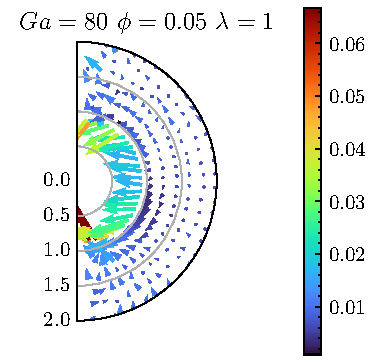
\includegraphics[width=0.3\textwidth]{image/HOMOGENEOUS_final/Dist/F_rel_l_1_Ga_80_PHI_5}
        \caption{Averaged force vector applied on the droplet present at the origin, conditioned on the presence of a nearest neighbor.
        The radial distance is made dimensionless by the droplets' diameter. 
        The color map represents the magnitude of the forces.}
        \label{fig:perspective_forces}
    \end{figure}
    On \ref{perspective_forces} we display our first result regarding the interaction forces statistic. 
    According to \citet{zhang2021ensemble} one remark \ref{fig:perspective_forces} is exactly a visual representation of teh particle-fluid-particle stress. 
    \item Altrough the most relevent closure of the continuous phase equations have been treated in this PhD work (Reynolds stress, drag force and stresslet), the closure terms of the disperse phase, specifically the particles center of mass velocity fluctuation $\pavg{\textbf{u}_\alpha'\textbf{u}_\alpha'}$, that is still need to be modeled. 
    Using a combination of Neast-Particle statistics and reflection method it is actually possible to derive an analytical model in the Stokes and Dilute regime. 
    The methodology is very similar to what is done in \ref{chap:pseudoturbulence}. 
    The first results gives, 
    \begin{equation*}
        \pavg{\textbf{u}_\alpha'\textbf{u}_\alpha'}
        % = 
        % n_p[\textbf{x},t]
        % \int_{\mathbb{R}^3}
        % (\textbf{v}^\text{nst}_p
        % \textbf{v}^\text{nst}_p)[\textbf{x},\textbf{y},t]
        % P_\text{nst}[\textbf{y}|\textbf{x},t]
        % d\textbf{y}
        = 
        C_1[\textbf{u}_{fp}\textbf{u}_{fp} - \frac{1}{3}(\textbf{u}_{fp}\cdot \textbf{u}_{fp})\bm\delta] 
        + C_2(\textbf{u}_{fp}\cdot \textbf{u}_{fp})\bm\delta
    \end{equation*}
    \begin{align}
      C_1 = \frac{1}{960}\left(\frac{2+3\lambda}{\lambda+1}\right)^2 \left[
        108\Gamma(1/3)
        - 80\Gamma (4/3)
        +15\Gamma(7/3)
      \right]\phi^{2/3}\\
      C_2 = \frac{1}{576}\left(
        \frac{2+3\lambda}{\lambda+1}\right)^2 \left[
        24\Gamma(1/3)
        - 16\Gamma (4/3)
        +3\Gamma(7/3)
      \right]\phi^{2/3}
    \end{align}
    For solid particle ($\lambda=\infty$) we find $\sqrt{k_p} = 1.52\phi^{1/3}$, while the experimental results reported in \citet{guazzelli2011fluctuations} suggest $\sqrt{k_p} = 2\phi^{1/3}$ and $3\phi^{1/3}$ which is higher. 
    First results are promising, more work on this topic is clearly needed.
    This study might lead to solve the famous Carlfish-Luke paradox \citet{caflisch1985variance}. 
\end{enumerate}

\paragraph*{Might be necessary}
Then there is points that might be relevant for this work, however at this stage it is hard to estimate the acctual needs.
\begin{enumerate}
    \item Another point of major importance not presented in this manuscript is the study of particle-fluid-particle stress, or long range interaction stress. 
    According to \cite{Lhuillier_2009,nott2011suspension,zhang2021ensemble} the drag force term can be expressed as a pure drag force term (that is the closure provided in \ref{chap:mono-disperse}) plus the divergence of a stress, the so-called particle-fluid-particle stress. 
    The latter stress would be responsible (among other term), for particle migration phenomenon.  
    At this stage it is hard to estimate if this stress is more or less important than the center of mass velocity variance, anyhow studies remain to be done to determine this contribution. 
    \item More generally up to know we considered homogeneous rising emulsion, however it might be relevant to take in account gradient of particle concentration in all of our closure terms. 
    The recent study of \citet{wang2024effect} started to include the gradient of volume fraction in the drag force closure. 
    \item Although we studied the first moment of hydrodynamic at low but finite inertial effect, it seems important to develop a model that is valid at higher Reynolds number and volume fraction since it seems that it could have a predominant effect on the stress in dense regime. 
    This can be carried out using the same DNS as presented in this work. 
    \item The study of the second moment of the hydrodynamic forces seems absent of the literature, while in our case where the flotation effects are dominant it remains important. 
    \item Finally, all of our closure terms consider a steady-state situation, meaning that we neglect the contribution from dispersed or continuous phase acceleration in our closure. 
    For the drag force this would correspond to added mass effect and that is known to be important. 
    For the other moment of forces this kind of contribution must be determined as well in terms of the unknowns of the problem. 
\end{enumerate}
These points mainly concerns the needs in closure models, a more general and thecnical conclusion on the closure model of the momentum equaitons is provided in \ref{ap:momentum_formulation} 


\paragraph*{Ideas of reaserch topics}
Now we would like to mention some ideas that seem pertinent for the modeling of multi-phase flow. 
\begin{enumerate}
    \item PR-DNS can be quite expansive to develop closure. 
    Thus, one might consider solving the single-particle conditioned averaged equations to produce closure.  
    Indeed, as demonstrated by \citet{hinch1977averaged} by considering closure within those equaitons one is able to derive more completet closure term, such as the second oreder correction of the equivalent stress and sedimentation velocity in this case. 
    Nevertheless, this approch is theoritically difficult, limiting the number of problem that can be traeated. 
    Solving this equation using numerical approach would enable us to consider more complicated scenario. 
    For example we could prescribe a given pair-distribution in the equations leading to closure model in terms of that pair-distribution; that could represent mean gradient of volume fraction, layers in the microstructure etc\ldots. 
    \item A second idea that seem relevant, is the use of the volume-averaged momentum bulk-equations presented in \ref{chap:daniel15} instead of the continuous phase averaged equation commonly used to describe the continuous phase momentum.
    This is interesting since this equations has the same form as classical N-S equaitons enabling us to use the single phase NS solver to describe the bulk-phase. 
    A set of equations for the dispersed phase is then added following the usual procedure. 
    A summary of this approach is given in \ref{ap:momentum_formulation}. 
\end{enumerate}




\addcontentsline{toc}{chapter}{Bibliography}
\bibliography{Bib/bib_bulles.bib}
\appendix
\addcontentsline{toc}{chapter}{Appendix }

\chapter{A detailed derivation of the \textit{one-fluid}, \textit{two-fluid} and volume averaged formulation of a generalized balance equations.}
\label{ap:average}

\section{General balance equations}

\begin{figure}[h]
    \centering
    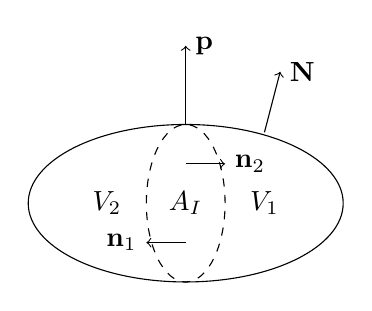
\begin{tikzpicture}
        \draw (0,0) ellipse (2 and 1);
        \draw[dashed] (0,0) ellipse (0.5 and 1)node{$A_I$};
        \draw[->](0,1)--++(0,1)node[right]{\textbf{p}}; 
        \draw[->](1,0.9)--++(0.2,0.77)node[right]{\textbf{N}}; 
        \draw[->](0,-0.5)--++(-0.5,0)node[left]{$\textbf{n}_1$}; 
        \draw[->](0,0.5)--++(0.5,0)node[right]{$\textbf{n}_2$}; 
        \draw (1,0)node{$V_1$};
        \draw (-1,0)node{$V_2$};
    \end{tikzpicture}
    \caption{Scheme of an arbitrary material control volume.   }
\end{figure}

Let $f^0$  be an arbitrary quantity to be conserved inside the non-material volume $\omega$. 
Then $\bm\Phi^0$ refer to the non-convective flux of $f^0$. 
Then $s^0$ refer to source term  related to  $f^0$. 
Then, for an arbitrary control volume we have, 
\begin{equation*}
    \ddt \int_{V} f^0 dV 
    = 
    \int_{V} s^0 dV 
    + \int_{\partial V} \mathbf{\Phi}^0 \cdot \textbf{N} dS,
\end{equation*}
where $\textbf{N}$ is the normal of the control volume. 
Any quantities defined in $V_k$ will be noted with a subscript $_k$ and those who are defined at the interface with $_I$. 
Therefore, if we decompose any quantity such as $f^0 = \sum_k f_k^0 \chi_k + f_I^0 \delta_I$ we obtain, 
\begin{multline*}
    \sum_k\left[\ddt \int_{V_k} f_k^0 dV 
    - \int_{V_k} s_k^0 dV 
    - \int_{A_k} \mathbf{\Phi}_k^0 \cdot \textbf{N} dS
    \right]
    + \ddt \int_{A_I} f_I^0 dS 
    - \int_{A_I} s_I^0 dS 
    - \int_{C} \mathbf{\Phi}_I^0 \cdot \textbf{p} dC 
    = 0
\end{multline*}
Using the Reynolds transport theorem on volume integral yields,
\begin{align*}
    \ddt \int_{V_k} f_k^0 dV 
    &= \int_{V_k} \pddt f_k^0 dV 
    + \int_{A_I \cup A_k} f_k^0 \textbf{u} \cdot \textbf{n}_k dS\\
    &= \int_{V_k} \left[
        \pddt f_k^0  + \div (f_k^0 \textbf{u}_k^0) 
    \right]dV 
    + \int_{A_I} f_k^0 (\textbf{u}_I^0 - \textbf{u}_k^0) \cdot \textbf{n}_k dS\\
\end{align*}
where $\textbf{n}_k$ is the normal of the interface $A_I$ on the outward direction of the $k$ phase. 

The second term is integrated only over $A_I$ as it is the interface between both phase and not the one of the control volume. 
Using the Ledbiz rule for integration on surface yields, 
\begin{align*}
    \ddt \int_{A_I} f_I^0 dS 
    &= \int_{A_I} \left[
        \pddt f_I^0  + \divI (f_I^0 \textbf{u}_I^0) 
    \right]dS
\end{align*}

Regarding the non-convective integrals, by using the divergence theorem we can write\citep{nadim1996concise}, 
\begin{align*}
    \int_{A_k} \mathbf{\Phi}_k^0\cdot \textbf{n}_k dS
    = \int_{V_k} \div\mathbf{\Phi}_k^0 dV
    - \int_{A_I} \mathbf{\Phi}_k^0\cdot \textbf{n}_k dS. 
\end{align*}
The last term can also be re-written with the divergence theorem \citet{nadim1996concise},
\begin{align*}
    \int_{C} \mathbf{\Phi}_I^0\cdot \textbf{p} dC 
    = \int_{A_I} \divI \mathbf{\Phi}_I^0 dS
    - \int_{A_I} \mathbf{\Phi}_I^0 \cdot \textbf{n} \div \textbf{n} dS
\end{align*}
Notice that whether it is $\textbf{n}_1$ or $\textbf{n}_2$ the second term on the left conserve the same sign. 

Taking in account these reformulations, we can re-write the integral balance previously exposed by, 
\begin{align*}
    \sum_k \int_{V_k}{\left[
        \pddt f_k^0
        + \div (f_k^0\textbf{u}_k^0 - \bm\Phi_k^0)
        - s_k^0
    \right]}\\
    + \sum_k\int_{A_I}{\left[
        f_k^0(\textbf{u}_I^0 - \textbf{u}_k^0)
        + \bm\Phi_k^0
    \right]\cdot \textbf{n}_k}
    + \int_{A_I}{\left[
        \pddt f_I^0 
        + \divI (f_I^0 \textbf{u}_I - \bm\Phi_I^0)
        + \bm\Phi_I^0 \cdot \textbf{n} \div \textbf{n}
    \right]} =0 
\end{align*}

Every integral of volume must be balanced independently of the surface integral. 
This means that we can separate this equation into two, 
\begin{equation*}
    \pddt f_k  
    + \div (f_k \textbf{u}_k - \mathbf{\Phi}_k) 
    =s_k. 
\end{equation*}
\begin{equation}
    \pddt f_I  
    + \divI (f_I \textbf{u}_I -\mathbf{\Phi}_I)
    + \mathbf{\Phi}_I \cdot \textbf{n} \div \textbf{n}
    = 
    + s_I
    - \sum_k \left[
    f_k (\textbf{u}_I - \textbf{u}_k)
    + \mathbf{\Phi}_k
    \right] \cdot \textbf{n}_k. 
    \label{ap:eq:dt_f_I}
\end{equation}
These equations are valid in $\Omega_k(t)$ and $\Sigma(t)$ for volume and surface quantity, respectively. 

Now let's reformulate the third term of the surface balance equation. 
Let $\textbf{F}$ be an arbitrary surface quantity. 
It can be split into two part such as, 
\begin{equation*}
    \textbf{F} 
    = \textbf{F} \cdot \textbf{n}\textbf{n}
    + (\textbf{I} - \textbf{nn})  \cdot \textbf{F}
    = \textbf{F}_\bot + \textbf{F}_{||}.
\end{equation*}
Injecting this decomposition inside the Gauss theorem on an arbitrary control volume it can be shown that, 
\begin{equation*}
    \int_{S} \divI \textbf{F}dS
    = 
    \int_{S} \left[\divI \textbf{F}_{||} 
    + \textbf{F} \cdot \textbf{n} \div\textbf{n}
    \right]dS
\end{equation*}
Consequently, we have the following relation,
\begin{equation*}
    \int_{A_I} \divI \bm\Phi_I^0dS
    = 
    \int_{A_I} \left[\divI \bm\Phi_{I||}^0
    + \bm\Phi_I^0 \cdot \textbf{n} \div\textbf{n}
    \right]dS
\end{equation*}

By taking in account this relation it is easy to take or not the normal components of a vector to the interface within the balance equaitons. 
For example, we can write either, 
\begin{equation}
    \pddt f_I  
    + \divI (f_I \textbf{u}^I_{||} -\mathbf{\Phi}^I_{||})
    + f_I \textbf{u}_I \cdot \textbf{n} \div \textbf{n}
    - s_I
    = 
    - \sum_k \left[
    f_k (\textbf{u}_I - \textbf{u}_k)
    + \mathbf{\Phi}_k
    \right] \cdot \textbf{n}_k 
    \label{ap:eq:dt_f_I2}
\end{equation}
Or 
\begin{equation}
    \pddt f_I  
    + \divI (f_I \textbf{u}^I -\mathbf{\Phi}^I_{||})
    - s_I
    = 
    - \sum_k \left[
    f_k (\textbf{u}_I - \textbf{u}_k)
    + \mathbf{\Phi}_k
    \right] \cdot \textbf{n}_k 
    \label{ap:eq:dt_f_I2}
\end{equation}
where we have changed the flux term formulation. 



\section{Topological equations}
There is two Topological equaitons one for $\chi_k$ and an other for $\delta_I$.
First, we recall the relations related to the phase indicator function, 
\begin{equation}
    \frac{\partial}{\partial t} \chi_k
    + \textbf{u}_I  \nablabh \chi_k 
    = 0, \;\;\;\;\text{and}\;\;\;\; 
    \nablabh \chi_k 
    = - \delta_I \textbf{n}_k.
    \label{ap:eq:phase_properties}
\end{equation}
Now the surface indicator function transport equation can be obtained using the Leibniz rule for differentiation,  
\begin{equation*}
    \ddt \int_{A_I} dS
    = \int_{A_I} \nablabh_I \cdot \textbf{u}_I dS,
\end{equation*}
Those integrals can be re rewritten as, 
\begin{equation*}
    \ddt \int_{V} \delta_I dV
    = \int_{V} \delta_I \nablabh_I \cdot \textbf{u}_I dV.
\end{equation*}
Then using the Reynolds transport term for fixed material volume yields,
\begin{equation*}
    \pddt \delta_I
    + \nablabh \cdot (\delta_I \textbf{u}_I)
    = \delta_I \nablabh_I \cdot \textbf{u}_I. 
\end{equation*}
This equation can also be takes the form 
\begin{equation}
    \pddt \delta_I
    + \nablabh \cdot (\delta_I \textbf{u}_I\cdot \textbf{n}\textbf{n})
    = \delta_I \textbf{u}_I \cdot \textbf{n}\nablabh \cdot \textbf{n}. 
    \label{ap:eq:dt_delta_I}
\end{equation}
Also, it can be useful to derive an expression for the gradient of the $\delta_I$ function. 
To do so we take the gradient of \ref{ap:eq:phase_properties} yielding, 
\begin{equation*}
    \nablabh\delta_I 
    = \nablabh( - \textbf{n}_k \cdot \nablabh \chi_k)
    = \nablabh\textbf{n}_k \cdot \textbf{n}_k \delta_I
    + \nablabh(\textbf{n}_k \delta_I) \cdot \textbf{n}_k 
\end{equation*}

\section{\textit{One-fluid} and \textit{two-fluid} formulations}
In this appendix we derive the \textit{two-fluid} and \textit{one-fluid} formulation of a generalized conservation equation, namely,
\begin{equation}
    \frac{\partial}{\partial t} f_k
    = \nablabh \cdot (\bm{\Phi}_k - f_k\textbf{u}_k)
    + \textbf{S}_k.
    \label{ap:eq:global_balance}
\end{equation}
Then we derive the phase averaged and global averaged equation of this general equation of conservation. 

We can derive the \textit{two-fluid} formulation by multiplying \ref{ap:eq:global_balance} by the phase indicator function \ref{eq:phase_indicator}. 
It yields, 
\begin{equation*}
    \frac{\partial}{\partial t} (\chi_k f_k)
    = \nablabh \cdot (\chi_k \bm{\Phi}_k - \chi_k f_k \textbf{u}_k)
    + \chi_k \textbf{S}_k.
    + f_k \frac{\partial}{\partial t} \chi_k
    + \left(
        f_k \textbf{u}_k 
        - \bm{\Phi}_k
    \right) \cdot \nablabh \chi_k
    % \label{ap:eq:global_balance}
\end{equation*}
where we have included the phase function $\chi_k$ into the derivative operators. 
Now, using the \ref{ap:eq:phase_properties} we get, 
\begin{equation}
    \frac{\partial}{\partial t} (\chi_k f_k)
    = \nablabh \cdot (\chi_k \bm{\Phi}_k - \chi_k f_k \textbf{u}_k)
    + \chi_k \textbf{S}_k
    + \left[
        \bm{\Phi}_k 
        + f_k 
        \left(
            \textbf{u}_I
            - \textbf{u}_k
        \right) 
    \right]
    \cdot \textbf{n}_k \delta_I 
    \label{ap:eq:two-fluid_global}
\end{equation}
where the last term is the interfacial source term, such as the drag force if $f_k$ is the momentum or the mass transfer if $f_k$ is the density. 
In this equation notice that all quantities are factor of the phase indicator function $\chi_k$. 
So we transport $\chi_k f_k$ which is field quantity defined over the whole domain. 
Thus, \ref{ap:eq:two-fluid_global} is valid over the entire domain.   

Now, we define the jump condition across the interface or the surface transport equation as the sum of the interfacial term on each phase $k$. 
It can be obtained using  the transport of surface \ref{ap:eq:dt_f_I2}.
Indeed, multiplying \ref{ap:eq:dt_f_I2} by $\delta_I$ gives, 
\begin{equation}
    \pddt (f_I\delta_I)  
    = 
    + \nablabh \cdot (\delta_I \mathbf{\Phi}^I_{||} - \delta_I f_I \textbf{u}^I)
    +\textbf{S}_I \delta_I
    - \sum_k \left[
    f_k (\textbf{u}_I - \textbf{u}_k)
    + \mathbf{\Phi}_k
    \right] \cdot \textbf{n}_k \delta_I
    \label{ap:eq:general_jump}
\end{equation}
\tb{
    Notice that the first term on the RHS is the parallele component of $\mathbf{\Phi}$ thus it must be reformulated as, 
    
}

Now, let's derive the \textit{one-fluid} formulation of the general conservation law.
To do so we sum on all phases \ref{ap:eq:two-fluid_global} plus the interface. 
Besides, we define any quantities $q$ such as, $q = \sum_k \chi_k q_k + \delta_I q_I$.
Then it is trivial to show that, 
\begin{equation}
    \frac{\partial}{\partial t} f
    = \nablabh \cdot (\bm{\Phi} - f \textbf{u})
    + \textbf{S}
    \label{ap:eq:one-fluid_global}
\end{equation}
which is the \textit{one-fluid} formulation. 

The volume average of \ref{ap:eq:two-fluid_global} is then straight forward, by using the definition of the averaged operator, we get, 
\begin{equation*}
    \frac{\partial}{\partial t} (\phi_k\kavg{f})
    = \nablabh \cdot \left(
        \phi_k \kavg{\bm{\Phi} - f \textbf{u}}
    \right)
    + \phi_k \kavg{\textbf{S}}
    + a_I \Iavg{
        \bm{\Phi}_k \cdot \textbf{n}_k
        + f_k 
        \left(
            \textbf{u}_I
            - \textbf{u}_k
        \right) \cdot \textbf{n}_k
    } 
\end{equation*}
Similarly, the bulk average can be obtained by averaging \ref{ap:eq:one-fluid_global} yielding, 
\begin{equation*}
    \frac{\partial}{\partial t} \avg{f}
    = \nablabh \cdot \avg{\bm{\Phi} - f \textbf{u}}
    + \avg{\textbf{S}}
    % + a_I\avg{\textbf{J}_I},
    \label{ap:eq:avg_global}
\end{equation*}
\section{Derivation of the point velocity}
Consider a particle of center of mass $\textbf{y}_\alpha$ defined such as
\begin{equation*}
    m_\alpha \textbf{y}_\alpha
    = \int_{V_\alpha} \rho_k \textbf{y}_k dV,
\end{equation*}
its velocity can be solely the derivation of $\textbf{y}_\alpha$ whitin time.
Yielding, 
\begin{align*}
    \ddt \textbf{y}_\alpha (t)
    &=
    \ddt \left(
        \frac{1}{m_\alpha} \int_{V_\alpha} \rho_k \textbf{y}_k dV
    \right)\\
    &= \frac{1}{m_\alpha}
    \ddt 
    \left(
        \int_{V_\alpha} \rho_k \textbf{y} dV
    \right)
    - \frac{1}{m_\alpha^2} \ddt \int_{V_\alpha} \rho_k dV \int_{V_\alpha} \rho_k \textbf{y}_k dV
    \\
    &= \frac{1}{m_\alpha}\int_{V_\alpha} \left[
        \pddt (\rho_k \textbf{y}) + \nablabh \cdot\left(\rho_k \textbf{y}\textbf{u}_k\right) dV 
    \right]\\
    &+ \frac{1}{m_\alpha}\int_{S_\alpha} \textbf{y} M_k d S
    -  \frac{1}{m_\alpha^2} \int_{S_\alpha} M_k dS  \int_{V_\alpha} \rho_k \textbf{y}_k dV
    \\
    &= \frac{1}{m_\alpha}\int_{V_\alpha} \textbf{y} \left[
    \pddt (\rho_k) + \nablabh \cdot\left(\rho_k \textbf{u}_k\right) dV 
    \right]dV
    + \frac{1}{m_\alpha}\int_{V_\alpha} \rho_k  \textbf{u}_k  \cdot \nablabh \textbf{y} dV \\
    &+ \frac{1}{m_\alpha}\int_{S_\alpha} \textbf{y}_k M_k d S
    - \frac{1}{m_\alpha}  \textbf{y}_\alpha \int_{S_\alpha} M_k dS
\end{align*}
By considering the mass conservation \ref{eq:single-fluid_mass} for the first term,  noticing that $\nablabh \textbf{y} = \textbf{I}$ where $\textbf{I}$ is the identity tensor for the second term and introducing \textbf{r} in the third term gives, we get the following relation,
\begin{equation*}
    \textbf{u}_\alpha
    = \frac{1}{m_\alpha} \left(
        \textbf{p}_\alpha
        +  \int_{S_\alpha} \textbf{r} M_k dS
    \right)
    % = \frac{1}{m_\alpha}  \left(
    %     \textbf{p}_\alpha
    % - \int_{V_\alpha} \rho_k \textbf{w} dV
    % \right)
\end{equation*}

\section{Derivation of the surface transport equations for Lagrangian particles}

By making use of the Leibniz rule together with \ref{ap:eq:dt_f_I} it can be shown that for any surface quantity $f_I$ we have, 
\begin{align*}
    \ddt \int_{S_\alpha} f_I dS
    &= \int_{S_\alpha} \pddt f_I 
    + \nablabh_I \cdot (\textbf{u}_If_I) dS\\
    &= \int_{S_\alpha} \left(
        \nablabh_I \cdot \mathbf{\Phi}_{||}^I
        + \textbf{S}_I
    \right) dS\\
    & - \sum_k \int_{S_\alpha} \left[
        f_k (\textbf{u}_I - \textbf{u}_k)
        + \mathbf{\Phi}_k
    \right] \cdot \textbf{n}_k
    dS
\end{align*}
Then remark that if $\mathbf{\Phi} = \sigma (\textbf{I}-\textbf{nn})$.
Then, 
\begin{equation*}
    \int_S \nablabh_I \cdot \left[\sigma (\textbf{I} - \textbf{nn})\right]dS 
    =
    \int_S  \nablabh_I \sigma dS 
    + \int_S \sigma \kappa \textbf{n}dS 
    = 0
\end{equation*}

Using the Gauss theorem for closed surface it can be shown easily that the first term on the RHS can be reformulated, leaving with, 
\begin{align}
    \ddt \int_{S_\alpha} f_I dS
    = \int_{S_\alpha} \left[
        \textbf{S}_I 
        - \kappa \mathbf{\Phi}_{||}^I\cdot \textbf{n} 
    \right]dS
    - \sum_k \int_{S_\alpha} \left[
        f_k (\textbf{u}_I - \textbf{u}_k)
        + \mathbf{\Phi}_k
    \right] \cdot \textbf{n}_k
    dS
\end{align}
In this equation we can see that $\mathbf{\Phi}_I$ plays no role at all. 

Now let's derive the first moment of a surface quantity, namely $f_I \textbf{r}$. 
\begin{align*}
    \ddt \int_{S_\alpha} f_I \textbf{r} dS
    &= \int_{S_\alpha} \textbf{r}\left[
        \pddt f_I 
        + \nablabh_I \cdot (\textbf{u}_If_I) 
    \right]dS
    + \int_{S_\alpha}
    f_I \left[
        \pddt \textbf{r} + \textbf{u}_I \cdot \nablabh_I \textbf{r}
    \right]
    dS\\
\end{align*}
Using \ref{ap:eq:dt_f_I} on the first term of the RHS and the relation $\nablabh_I \textbf{r} = (\textbf{I} - \textbf{nn})$ gives, 
\begin{align*}
    \ddt \int_{S_\alpha} f_I \textbf{r} dS
    &= \int_{S_\alpha} \textbf{r}\left[
        \nablabh_I \cdot \mathbf{\Phi}_I
        - \Phi_I\cdot\textbf{n}\nablabh\textbf{n}
        + \textbf{S}_I
    \right] dS\\
    & - \sum_k \int_{S_\alpha}\textbf{r} \left[
        f_k (\textbf{u}_I - \textbf{u}_k)
        + \mathbf{\Phi}_k
    \right] \cdot \textbf{n}_k
    dS\\
    &+ \int_{S_\alpha}
    f_I (\textbf{u}^I_{||} - \textbf{u}_\alpha)
    dS\\
\end{align*}
Using the Gauss theorem for closed surface on the first term on the RHS, this equation can be simplified to, 
\begin{align}
    \ddt \int_{S_\alpha} f_I \textbf{r} dS
    &= \int_{S_\alpha} \left(
        \textbf{S}_I\textbf{r}
        - \mathbf{\Phi}_{||}^I
    \right) dS
    + \int_{S_\alpha}
    f_I \textbf{w}_I
    dS\nonumber\\
    & - \sum_k \int_{S_\alpha}\textbf{r} \left[
        f_k (\textbf{u}_I - \textbf{u}_k)
        + \mathbf{\Phi}_k
    \right] \cdot \textbf{n}_k
    dS
    \label{ap:eq:dt_r_f_I}
\end{align}
where $\textbf{w}_{I||} = \textbf{u}_{I||} - \textbf{u}_\alpha$. 
In the jump condition of the first moment it is now evident that $\mathbf{\Phi}^I_{||}$ is relevant. 

As an example, if $f_I$ were to be the momentum of the surface, then $\mathbf{\Phi}_{||}^I = \sigma (\textbf{I} - \textbf{nn})$. 
Thus, we can express the integrals as, 
\begin{equation*}
    \int_{S_\alpha}\mathbf{\Phi}_{||}^IdS
    =\int_{S_\alpha} \sigma (\textbf{I} - \textbf{nn}) dS
    =\int_{S_\alpha} \nablabh_I \cdot (\sigma \textbf{r}) dS
    =\int_{S_\alpha} \sigma \textbf{r} (\nablabh\cdot\textbf{n}) \textbf{n} dS
\end{equation*} 
where we used the Gauss theorem on closed surface for the first term. 
In this last expression we recognize the last term as begin the first moment of the surface tension force. 




\section{Decomposition of the particular energy balance.}
This section is a detailed derivation of the energy equation for a whole fluid particle, namely,
\begin{equation*}
    \label{ap:eq:E_alpha_dt}
    \ddt E_\alpha 
    % = \ddt \int_{V_\alpha} \rho_k E_k dV
    = \int_{V_\alpha} \textbf{b}_k \cdot \textbf{u}_k dV
    + \int_{S_\alpha} \left[
        (\textbf{T}\cdot \textbf{u} 
    - \textbf{q})\cdot\textbf{n}_k 
    + M_k E_k 
    + \textbf{f}_I \cdot \textbf{u}_I 
    \right]dS, 
\end{equation*}
Since we can decompose the velocity fields of a particle following $\textbf{u}_k = \textbf{u}_\alpha + \textbf{w}$ it is then possible to rewrite the total energy, 
Yielding, 
\begin{multline*}
    \int_{V_\alpha} \rho_k E_k dV
    = \int_{V_\alpha} \rho_k e_k dV
    + \frac{1}{2} \int_{V_\alpha} \rho_k \textbf{u}_\alpha\cdot\textbf{u}_\alpha dV\\
    + \int_{V_\alpha} \rho_k \textbf{u}_\alpha\cdot\textbf{w} dV
    + \frac{1}{2} \int_{V_\alpha} \rho_k \textbf{w}\cdot\textbf{w} dV
\end{multline*}
by applying the relation \ref{eq:M_alpha_dt} on the second term, it is possible to show that,
\begin{equation*}
    E_\alpha
    = \int_{V_\alpha} \rho_k e_k dV
    + \frac{1}{2} \textbf{u}_\alpha\cdot\textbf{u}_\alpha  m_\alpha
    + \textbf{u}_\alpha\cdot \int_{V_\alpha} \rho_k \textbf{w} dV
    + \frac{1}{2} \int_{V_\alpha} \rho_k \textbf{w}\cdot\textbf{w} dV.
\end{equation*}
We clearly see that the energy can be decomposed into internal and kinetic energy. 
We define the integrated internal energy of the particle by $e_\alpha = \int_{V_\alpha} = \rho_k e_k dV$.
It is the straight forward (using \ref{eq:one-fuild_internal_energy}) to show that, 
\begin{equation*}
    \ddt e_\alpha
    = \int_{V_\alpha} \textbf{T}:\nablabh\textbf{u}_k dV
    + \int_{S_\alpha} \left(
        e_k M_k
        - \textbf{q}_k \cdot \textbf{n}_k
    \right) dS.
\end{equation*}
Similarly, the kinetic energy equation for a whole fluid particle can be obtained deriving the local kinetic energy ,namely,
\begin{equation*}
    \ddt \int_{V_\alpha} \rho_k \frac{u_k^2}{2} dV
    = \int_{V_\alpha}\textbf{u}_k \cdot  \left(
        \textbf{b}_k
        + \nablabh \cdot \textbf{T}_k
    \right)dV
    + \int_{S_\alpha} \frac{u_k^2}{2} M_k dS.
\end{equation*}
Using the velocity decomposition one can deduce, 
\begin{multline}
    \frac{1}{2} \ddt \left(
        m_\alpha \textbf{u}_\alpha \cdot \textbf{u}_\alpha
        + 2\textbf{u}_\alpha \cdot \int_{V_\alpha}  \rho_k \textbf{w}_k dV
        + \int_{V_\alpha} \rho_k \textbf{w}_k \cdot \textbf{w}_k dV
    \right)\\
    =  \textbf{u}_\alpha \left[
        \cdot\int_{V_\alpha} \textbf{b}_k dV
        +  \int_{S_\alpha} \left(
            \textbf{T}_k \cdot \textbf{n}_k
            + \frac{1}{2} \textbf{u}_\alpha M_k 
            + \textbf{w}_k M_k 
        \right)dS
    \right]\\
    + \int_{V_\alpha} \left(
        \textbf{w}_k\cdot\textbf{b}_k
        -\textbf{T}_k : \nablabh \textbf{w}_k
    \right)dV
    + \int_{S_\alpha} 
        \textbf{w}_k\cdot(\textbf{T}_k\cdot \textbf{n}_k)
    dS\\
    + \int_{S_\alpha} \frac{1}{2} \textbf{w}_k \cdot \textbf{w}_k M_k dS.
    \label{ap:eq:u_2_dt}
\end{multline}
Besides, taking the dot product of the centered velocity $\textbf{u}_\alpha$, with the momentum equation \ref{eq:dt_p_alpha}, gives, 
\begin{multline*}
    \frac{1}{2}\ddt (m_\alpha \textbf{u}_\alpha \cdot \textbf{u}_\alpha)
    + \textbf{u}_\alpha \cdot \ddt \int_{V_\alpha} \rho_k \textbf{w}_k dV \\
    = \textbf{u}_\alpha \cdot \int_{V_\alpha} \textbf{b}_k dV
    + \textbf{u}_\alpha \cdot \int_{S_\alpha} \left(
    \textbf{T}_k \cdot\textbf{n}_k
    +\frac{\textbf{u}_\alpha}{2} M_k
    +\textbf{w}_k M_k
    \right)dS,
\end{multline*}
We can notice that the RHS of this equation correspond rigorously to the second line of \ref{ap:eq:u_2_dt}.
Therefore, taking the difference between those equations, yields the internal motion equation of an arbitrary particle, namely, 
\begin{multline*}
    \frac{1}{2}\ddt \int_{V_\alpha} \frac{\rho_k}{2} \textbf{w}_k \cdot \textbf{w}_k dV
    = \int_{V_\alpha} \left(
        \textbf{w}_k\cdot\textbf{b}_k
        -\textbf{T}_k : \nablabh \textbf{w}_k
    \right)dV\\
    + \int_{S_\alpha} 
        \textbf{w}_k\cdot(\textbf{T}_k\cdot \textbf{n}_k)
    dS
    + \int_{S_\alpha} \frac{1}{2} \textbf{w}_k \cdot \textbf{w}_k M_k dS.
\end{multline*}

\section{Derivation of kinetic Turbulence Evolution Equations}

The aim of this section is to derive the transport equation for the granular temperature scalar. 
Let's define the grain temperature, $T$ as such, $T =\frac{1}{2} \textbf{u}'\cdot\textbf{u}'$, where $\textbf{u}'$ is the fluctuation velocity of a given average procedure. 

\subsection{For a continuous phase}
We start this derivation for the continuous phase $k$, so that $\textbf{u}'_k = \textbf{u}_k - \kavg{\textbf{u}}$.
We start from the averaged kinetic energy equation over the $k$ phase, namely : 
\begin{multline*}
    \frac{\rho_k}{2}\frac{\partial }{\partial t}\left(
        \phi_k
        \kavg{u^2}
    \right)
    +\frac{\rho_k}{2}\nablab\cdot \left(
        \phi_k
        \kavg{u^2\textbf{u}}
    \right)
    =
    \nablab\cdot\left(
        \phi_k
        \kavg{\textbf{u}\cdot \textbf{T}}
    \right)
    +\phi_k\kavg{\textbf{u}\cdot\textbf{b} - \textbf{T}: \nablabh\textbf{u}}\\
    +a_I \Iavg{
        (\textbf{T}_k\cdot\textbf{u}_k)\cdot\textbf{n}_k
        + \frac{u^2_k}{2} M_k}.
\end{multline*}
Breaking down the LHS of this equation times $\frac{2}{\rho_k}$, yields,
\begin{align*}
    &\frac{\partial }{\partial t}\left(
        \phi_k
        \kavg{u^2}
    \right)
    +
    \nablab\cdot \left(
        \phi_k
        \kavg{u^2\textbf{u}}
    \right)\\
    &=
    \phi_k\frac{\partial }{\partial t}\kavg{u^2}
    +\kavg{u^2}\frac{\partial }{\partial t}\phi_k
    +\nablab\cdot \left(
        \phi_k
        \kavg{u^2}\kavg{\textbf{u}}
        +\phi_k
        \kavg{u^2\textbf{u}'}
    \right)\\
    &=
    \phi_k
    \left[
        \frac{\partial }{\partial t}\kavg{u^2}
        + 
        \kavg{\textbf{u}}
        \cdot\nablab 
        \kavg{u^2}
    \right]
    +\kavg{u^2} \left[
        \frac{\partial }{\partial t}\phi_k
        + \nablab\cdot \left(
            \phi_k
            \kavg{\textbf{u}}
        \right)
    \right]\\
    &+ \nablab\cdot \left(
        2\phi_k
        \kavg{\textbf{u}}\cdot\kavg{\textbf{u'}\textbf{u'}} + \phi_k \kavg{T \textbf{u'}}
    \right)
\end{align*}
where we used $\kavg{u^2} = \kavg{u}^2 + T$. 
By using the averaged mass conservation \ref{eq:avg_k_mass} times $\frac{1}{2}\kavg{u^2}$, namely, 
\begin{equation*}
    \frac{\rho_k}{2} \kavg{u^2} \pddt \phi_k 
    + \frac{\rho_k}{2} \kavg{u^2} \nablab \cdot\left(\phi_k\kavg{\textbf{u}}\right)
    = \frac{a_I}{2}\kavg{u^2}\Iavg{M_k},
\end{equation*}
we can rewrite the energy balance in conservative form. 
It reads as, 
\begin{multline}
    \phi_k\frac{\rho_k}{2}  \left[
        \frac{\partial }{\partial t}
        \kavg{u^2}
        +\kavg{\textbf{u}}\cdot\nablab 
        \kavg{u^2}
    \right]
    =
    \nablab\cdot\left(
        \phi_k
        \kavg{\textbf{u}\cdot \textbf{T}
        - \rho_k\kavg{\textbf{u}}\cdot\textbf{u'u'}
        - \frac{\rho_k}{2}T\textbf{u'}}
    \right)\\
    +\phi_k\kavg{\textbf{u}\cdot\textbf{b} - \textbf{T}: \nablabh\textbf{u}}
    +a_I \Iavg{
        (\textbf{T}_k\cdot\textbf{u}_k)\cdot\textbf{n}_k
        + \frac{u^2_k - \kavg{u^2}}{2} M_k}.
    \label{ap:eq:avg_k_u_2}
\end{multline}
On the other hand the momentum equation reads as, 
\begin{multline*}
    \rho_k\pddt (\phi_k\kavg{\textbf{u}}) 
    + \rho_k\nablab\cdot(\phi_k\kavg{\textbf{u}}\kavg{\textbf{u}})\\
    = \nablab\cdot\left[
        \phi_k \kavg{\textbf{T}
        - \rho_k \textbf{u'u'}}
    \right]
    +\phi_k\kavg{\textbf{b}}
    + a_I\Iavg{M_k \textbf{u}_k +\textbf{n}_k\cdot\textbf{T}_k},
\end{multline*}
using the mass balance times $\kavg{\textbf{u}}$, we can write the momentum equation as, 
\begin{multline*}
    \rho_k \phi_k \left[
        \pddt \kavg{\textbf{u}}
        + \kavg{\textbf{u}}\cdot\nablab\kavg{\textbf{u}}
    \right]\\
    = \nablab\cdot\left[
        \phi_k \kavg{\textbf{T}
        - \rho_k \textbf{u'u'}}
    \right]
    +\phi_k\kavg{\textbf{b}}
    + a_I\Iavg{M_k \left(\textbf{u}_k - \kavg{\textbf{u}}\right) +\textbf{n}_k\cdot\textbf{T}_k}.
\end{multline*}
Then taking the dot product of this equation with $\kavg{\textbf{u}}$ gives, 
\begin{multline}
    \phi_k\frac{\rho_k}{2}  \left[
        \pddt \kavg{u}^2
        + \kavg{\textbf{u}}\cdot\nablab\kavg{u}^2
    \right]\\
    = \nablab\cdot\left[
        \phi_k \kavg{\textbf{u}}\cdot\kavg{\textbf{T}
        - \rho_k  \textbf{u'u'}}
    \right]
    +\phi_k\kavg{\rho_k \textbf{u'u'} - \textbf{T}}:\nablab
         \kavg{\textbf{u}}\\
    +\phi_k\kavg{\textbf{u}}\cdot\kavg{\textbf{b}}
    + a_I\Iavg{M_k \left(\textbf{u}_k\cdot\kavg{\textbf{u}} 
    - \kavg{u}^2\right) +\textbf{n}_k\cdot(\kavg{\textbf{u}}\cdot\textbf{T}_k)}.
    \label{ap:eq:avg_k_u_u}
\end{multline}
Finally, we can obtain the transport equation of $T$ by subtracting \ref{ap:eq:avg_k_u_2} with \ref{ap:eq:avg_k_u_u}. 
Yielding the following equation, 
\begin{multline}
    \phi_k\rho_k  \left[
        \frac{\partial }{\partial t}
        \kavg{T}
        +\kavg{\textbf{u}}\cdot\nablab 
        \kavg{T}
    \right]\\
    =
    \nablab\cdot\left(
        \phi_k
        \kavg{\textbf{u'}\cdot \textbf{T'}
        - \rho_k T\textbf{u'}}
    \right)
    +\phi_k\kavg{\rho_k \textbf{u'u'}}:\nablab
         \kavg{\textbf{u}}\\
    +\phi_k\kavg{\textbf{u'}\cdot\textbf{b'} + \textbf{T'}: (\nablabh\textbf{u})'}
    +a_I \Iavg{
        (\textbf{T}_k'\cdot\textbf{u}'_k)\cdot\textbf{n}_k
        + T M_k}.
    \label{ap:eq:avg_k_T}
\end{multline}


\subsection*{Dispersed phase}

In the same spirit as the previous section we carry out the derivation for the transport of the kinetic turbulence evolution $T$. 
The only difference is that $T$ is now defined relative to the mean velocity of the particular phase $\pavg{u}$.  
From the previous section we know that we can write the energy equation under the following form, 
\begin{multline*}
    \frac{1}{2}\ddt (m_\alpha u^2_\alpha)
    + \textbf{u}_\alpha \cdot \ddt \int_{V_\alpha} \rho_k \textbf{w}_k dV 
    = \textbf{u}_\alpha \cdot \int_{V_\alpha} \textbf{b}_k dV\\
    + \textbf{u}_\alpha \cdot \int_{S_\alpha} \left[
    \textbf{T}_k \cdot\textbf{n}_k
    +\frac{\textbf{u}_\alpha}{2} M_k
    +\textbf{w}_k M_k
    \right]dS.
\end{multline*}
Applying the particular average operator yields the averaged point of mass kinetic energy equation, 
\begin{multline*}
    \frac{1}{2}\pddt   \left(\pavg{m_\alpha} \pnavg{u^2_\alpha}\right)
    + \frac{1}{2}\nablab \cdot \left(\pavg{m_\alpha} \pnavg{u^2_\alpha \textbf{u}_\alpha}\right) 
    = \pavg{\textbf{u}_\alpha \cdot \int_{V_\alpha} \textbf{b}_k dV}\\
    - \frac{1}{2}\pddt \left(\pavg{m_\alpha'(u_\alpha^2)'}\right)
    - \frac{1}{2}\nablab\cdot\left(\pavg{m_\alpha' (u_\alpha^2 \textbf{u}_\alpha)'}\right)\\
    - \pavg{\textbf{u}_\alpha \cdot \ddt \int_{V_\alpha} \rho_k \textbf{w}_k dV} 
    + \pavg{\textbf{u}_\alpha \cdot \int_{S_\alpha} \left[
    \textbf{T}_k \cdot\textbf{n}_k
    +\frac{\textbf{u}_\alpha}{2} M_k
    +\textbf{w}_k M_k
    \right]dS}.
\end{multline*}
From this step, we can carry out the same decomposition as the previous section for the RHS/2. 
Namely, 
\begin{multline*}
    \frac{\partial }{\partial t}\left(
        \pavg{m_\alpha}
        \pnavg{u^2_\alpha}
    \right)+
    \nablab\cdot \left(
        \pavg{m_\alpha}
        \pnavg{u^2_\alpha\textbf{u}_\alpha}
    \right) \\
    =
    \pavg{m_\alpha}
    \left[
        \frac{\partial }{\partial t}\pnavg{u^2_\alpha}
        + 
        \pnavg{\textbf{u}_\alpha}
        \cdot\nablab 
        \pnavg{u^2_\alpha}
    \right]
    +\pnavg{u^2_\alpha} \left[
        \frac{\partial }{\partial t}\pavg{m_\alpha}
        + \nablab\cdot \left(
            \pavg{m_\alpha}
            \pnavg{\textbf{u}_\alpha}
        \right)
    \right]\\
    + \nablab\cdot \left(
        2\pavg{m_\alpha}
        \pnavg{\textbf{u}_\alpha}\cdot\pnavg{\textbf{u'}\textbf{u'}} 
        + \pavg{m_\alpha} \pnavg{T \textbf{u'}}
    \right)
\end{multline*}
As we can observe the possible polydispersity of the flow, add supplementary terms linked to the fluctuation of the mass, $m_\alpha'$.
The energy equations in the conservative form then reads as, 
\begin{multline*}
    \frac{\pavg{m_\alpha}}{2}
    \left[
        \frac{\partial }{\partial t}\pnavg{u^2_\alpha}
        + 
        \pnavg{\textbf{u}_\alpha}
        \cdot\nablab 
        \pnavg{u^2_\alpha}
    \right]
    = \pavg{\textbf{u}_\alpha \cdot \int_{V_\alpha} \textbf{b}_k dV} + \nablab \cdot \textbf{L}\\
    - \pavg{\textbf{u}_\alpha \cdot \ddt \int_{V_\alpha} \rho_k \textbf{w}_k dV} 
    - \pavg{u_\alpha^2}\pnavg{\int_{S_\alpha} M_k d S}\\
    + \pavg{\textbf{u}_\alpha \cdot \int_{S_\alpha} \left[
    \textbf{T}_k \cdot\textbf{n}_k
    +\frac{\textbf{u}_\alpha}{2} M_k
    +\textbf{w}_k M_k
    \right]dS},
\end{multline*}
where \textbf{L} represent all the fluctuation terms derived in the two previous equations. 

Now let's look at the particular averaged momentum equation. 
Using similar decomposition as in the previous part,
and by using the decomposition of the momentum, $\textbf{p}_\alpha = m_\alpha \textbf{u}_\alpha + \int_{V_\alpha} \textbf{w}_k dV$, the equation aforesaid reads as, 
\begin{multline*}
    \pavg{m_\alpha} \left[
        \pddt \pnavg{\textbf{u}_\alpha}
        + \pnavg{\textbf{u}_\alpha}\cdot\nablab\pnavg{\textbf{u}_\alpha}
    \right]
    = \pavg{\int_{V_\alpha} \textbf{b}_k dV}
    + \nablab \cdot \textbf{R}\\
    - \pavg{\ddt \int_{V_\alpha} \rho_k \textbf{w}_k dV} 
    + \pavg{\int_{S_\alpha} \left[\textbf{T}_k + \rho_k \textbf{u}_k (\textbf{u}_I-\textbf{u}_k) \right] \cdot \textbf{n}_k d S}
\end{multline*}
where \textbf{R} is the term that gather all the fluctuation terms. 
Multiplying, this equation by $\pnavg{\textbf{u}_\alpha}$ and taking the difference with the energy equation yielding, 
\begin{multline*}
    \frac{\pavg{m_\alpha}}{2}
    \left[
        \frac{\partial }{\partial t}\pnavg{T_\alpha}
        + 
        \pnavg{\textbf{u}_\alpha}
        \cdot\nablab 
        \pnavg{T_\alpha}
    \right]
    = \pavg{\textbf{u}_\alpha' \cdot \left(\int_{V_\alpha} \textbf{b}_k dV\right)'} 
    + \nablab \cdot \left(\textbf{L}-\textbf{R}\right)\\
    - \pavg{\textbf{u}_\alpha' \cdot \left(\ddt \int_{V_\alpha} \rho_k \textbf{w}_k dV\right)'} \\
    - \pavg{T_\alpha}\pnavg{\int_{S_\alpha} M_k d S}
    + \pavg{\textbf{u}_\alpha \cdot \int_{S_\alpha} \left[
    \textbf{T}_k \cdot\textbf{n}_k
    +\frac{\textbf{u}_\alpha}{2} M_k
    +\textbf{w}_k M_k
    \right]dS},
\end{multline*}
\chapter{Equivalence between volume average and weighted average for Lagrangian poly-disperse particles}
\label{ap:equivalence}
As mentioned in \ref{chap:avg} the velocity fields $\left<\bm{u}\right>^L_\gamma$ is needed in \ref{eq:PBM_QBMM}.
While, with the particular-average, \ref{eq:classic_hybrid_momentum_c}, we solve for $\left<\bm{u}\right>^p$.
Also, in \ref{eq:classic_hybrid_momentum_c} we have assumed an even distribution of particles size where this is clearly not the case. 
In the following we show the equivalence between the two averaged quantities and the correctness of the uniformity assumption. 
This appendix aim to prove rigorously the link between the population balance model and the particular-average equation.
The strategy is to derive \ref{eq:classic_hybrid_momentum_p} from Liouville equation following the method of \citet{curtiss1956kinetic} and \citet[chapter~7]{rao2008introduction}.
This way we show an equivalence by identification between the quantities mentioned above.

Let's consider the Boltzmann equation for a distribution $P(\textbf{x},\mathscr{C})$.
The distribution must remain physical, thus it must respect $\lim_{\mathscr{C} \rightarrow \partial\mathscr{C}} = 0$, where $\partial \mathscr{C}$ correspond to the boundary of the domain of definition of each component of $\mathscr{C}$. 
It yields, 
\begin{equation}
    \label{eq:Liouville}
    \pddt P(\textbf{x},\mathscr{C})
    + \bm{\nabla} \cdot \left(\textbf{u} P(\textbf{x},\mathscr{C})\right)
    + \grad_\mathscr{C} \cdot \left(\frac{d\mathscr{C}}{dt} P(\textbf{x},\mathscr{C})\right) 
    = \Psi
\end{equation}
Now let's consider a function $f(\mathscr{C},t)$ which represent any physical quantity function of the internal coordinate and the time. 
Multiplying \ref{eq:Liouville} by the function, $q_\alpha$, and integrating over all the internal coordinates yields Maxwell equation,
\begin{equation}
    \int q_\alpha \pddt P d\mathscr{C}
    + \int q_\alpha \grad \cdot \left(\textbf{u} P\right)d\mathscr{C}
    + \int q_\alpha \grad_\mathscr{C} \cdot \left(\frac{d\mathscr{C}}{dt} P\right) d\mathscr{C} = \int q_\alpha \Psi d\mathscr{C}.
\end{equation}
The first two terms derivative can be swapped with the integral since they are not function of $\mathscr{C}$.
Then, we make use of the divergence theorem on the third term, 
yielding,
\begin{multline}
    \pddt \int q_\alpha  P d\mathscr{C}
    + \grad \cdot\int q_\alpha \left(\textbf{u} P\right)d\mathscr{C} 
    % + \int_{\partial \lambda} \grad_\mathscr{C} \cdot \left(f \textbf{u}_\lambda P\right) d\partial\mathscr{C} 
    = \int q_\alpha \Psi d\mathscr{C},
    +\int \left(\frac{d\mathscr{C}}{dt} P\right) \cdot \grad_\mathscr{C} f  d\mathscr{C} 
    \label{eq:inttt}
\end{multline}
The second integral on RHS has been derived using the divergence theorem and considering that the distributions $P$ vanish near its boundaries. 
After applying the average operator \ref{eq:inttt} reads as,
\begin{equation}
    \pddt \left( n \avg{q_\alpha}\right)
    + \bm{\nabla} \cdot \left(n \avg{\textbf{u} q_\alpha}\right)
    = n \avg{\Psi q_\alpha}
    + n  \avg{\frac{d\mathscr{C}}{dt} \cdot \grad_\mathscr{C} q_\alpha}
    \label{ap:eq:maxwell}
\end{equation}
Note that up to now we have made no assumption on the shape of $P$ and on the nature of the internal coordinates $\mathscr{C}$. 
Nevertheless, only the number of particles  $n$, appear in \ref{ap:eq:maxwell}.
At this point of the development we must specify the nature of the internal coordinates.
Thus, in the next section we investigate different situation. 
In this context the scalar $\Psi$ represent the source term due to 3 things. 
The coalescence and break-up phenomena, and the inter particular collision. 
The source term can be thus expressed under this form \citep{rao2008introduction,curtiss1956kinetic},  
\begin{equation*}
    \Psi(\mathscr{C}) = B(\mathscr{C}) + D(\mathscr{C}) + \Pi(\mathscr{C}) + \nabla \cdot \Theta(\mathscr{C})
\end{equation*}
where $B$ is the birth term, $D$ the death term, $\Pi$ the collision source term, and $\Theta$ the collision flux. 

\section{Point mass particles}
We start by considering only point of mass particles. 
Therefore, we consider only the momentum of the particles $\textbf{p}_\alpha$ and the volume $V_\alpha$ as an internal coordinate.
Thus, \ref{ap:eq:maxwell} yields,
\begin{equation}
    \pddt \left( n \avg{q_\alpha}\right)
    + \bm{\nabla} \cdot \left(n \avg{q_\alpha \textbf{u}_\alpha}\right)
    - n  \avg{\frac{\partial V_\alpha}{\partial t} \cdot \frac{\partial q_\alpha}{\partial V_\alpha}}
    - n  \avg{\frac{\partial \textbf{p}_\alpha}{\partial t} \cdot \frac{\partial q_\alpha}{\partial \textbf{p}_\alpha}}
    = n \avg{\Psi q_\alpha},
\end{equation}
From this equation we can recover the conservation equations of the particular phase by replacing $q_\alpha$ by the right quantity. 
Consider, $f = 1$, for example, we get, 
\begin{equation}
    \pddt n
    + \grad \cdot \left(n \avg{\textbf{u}_\alpha}\right)
    = n\avg{\Psi}
\end{equation}
which is the conservation of the number density of the particles. 
Where the right-hand side is to coalesce and break up kernel.
Similarly, the mass balance equation can be obtained with $f = V_\alpha \rho_d$, yielding,
\begin{equation}
    \pddt (n\avg{m_\alpha})
    + \bm{\nabla} \cdot \left(n \avg{\textbf{u}_\alpha m_\alpha}\right)
    =
    n  \avg{\int_{S_\alpha} M_d dS},
\end{equation}
where we have use \ref{eq:dt_m_alpha} to make appear the mass transfer term. 
Note that the source term is null since coalescence and break-up conserve the mass. 
Again, for the momentum conservation equation we set $f = \textbf{p}_\alpha$.
\begin{equation}
    \pddt \left( n \avg{\textbf{p}_\alpha}\right)
    + \grad \cdot \left(n \avg{\textbf{u}_\alpha \textbf{p}_\alpha}\right)
    =  \nabla \cdot \Theta
    + n  \avg{\frac{\partial \textbf{p}_\alpha}{\partial t}}
\end{equation}
where $B$, $D$ and $\Pi$ cancel out since they doesn't change the momentum of the phase. 
Nevertheless, note that the collision flux term stay \citep{rao2008introduction}.
Using, the momentum balance for a single particle \ref{eq:dt_p_alpha}, we can simplify the last term yielding, 
\begin{multline*}
    \pddt \left( n \avg{\textbf{p}_\alpha}\right)
    + \bm{\nabla} \cdot \left(n \avg{\textbf{u}_\alpha \textbf{p}_\alpha }\right)\\
    = 
    \nabla \cdot \Theta
    + n\avg{\int_{V_\alpha} \textbf{b}_k dV}
    + \avg{\int_{S_\alpha} \left(
    \textbf{T}_k\cdot\textbf{n}_k
    - M_k \textbf{u}_k
    \right)dS},
\end{multline*}
The system of equation obtained here is equivalent to \ref{eq:avg_p_momentum}, but with an additional source $\Theta$ terms representing the particle stress.

We can also set $f = \textbf{u}_\alpha$ instead of $\textbf{p}_\alpha$ and consider only $\textbf{u}_\alpha$ as an internal coordinate.
Then by using \ref{eq:u_alpha_dt} we directly have, 
\begin{multline*}
    \pddt \left( n \avg{\textbf{u}_\alpha}\right)
    + \bm{\nabla} \cdot \left(n \avg{\textbf{u}_\alpha \textbf{u}_\alpha }\right)
    = 
    \nabla \cdot \Theta
    + n\avg{\frac{1}{m_\alpha}\int_{V_\alpha} \textbf{b}_k dV} \\
    + \avg{\frac{1}{m_\alpha}\int_{S_\alpha} \left(
    \textbf{T}_k\cdot\textbf{n}_k
    - M_k \textbf{w}_k
    \right)dS}
    + \avg{\frac{1}{m_\alpha} \ddt \int_{S_\alpha} 
        \textbf{r} M_k dS},
\end{multline*}

% \section{Higher order description of the particles}
% In the previous section we only considered the center of mass velocity.
% Here we consider also the first order moment of inertia and momentum.
% Therefore, we consider the following quantities as internal coordinate,
% the momentum $\textbf{p}_\alpha$, the moment of momentum $\mathcal{P}_\alpha$ and the moment of inertia $\mathcal{G}$.
% In the following we will adopt indices notation to be more rigorous. 
% Besides, we will neglect all terms related to the mass transfer.
% \ref{ap:eq:maxwell} now reads as, 
% \begin{multline*}
%     \pddt \left( n \avg{q_\alpha}\right)
%     + \frac{\partial}{\partial x_i} \left(n \avg{\textbf{u}_\alpha q_\alpha}\right) 
%     = n \left<Jf\right>^\lambda.\\
%     + n  \left<\frac{d p^\alpha_i}{dt} \frac{\partial q_\alpha}{\partial p_i} \right>^{\lambda} 
%     + n  \left<\frac{d\mathcal{G}^\alpha_{ij}}{dt} \frac{\partial q_\alpha}{\partial\mathcal{G}_{ij}}\right>^{\lambda} 
%     + n  \left<\frac{d\mathcal{P}^\alpha_{ij}}{dt} \frac{\partial q_\alpha}{\partial\mathcal{P}_{ij}}\right>^{\lambda} 
% \end{multline*}
% Now, we can apply the same process as earlier to get the conservation equations.
% For $f = \mathcal{G}_{ij}^\alpha$ we get,
% \begin{equation*}
%     \pddt \left( n \left<\mathcal{G}_{ij}\right>^\lambda\right)
%     + \frac{\partial}{\partial x_k} \cdot \left(n \left<\mathcal{G}_{ij} u_k^\alpha \right>^\lambda\right)
%     = n \left<J \mathcal{G}_{ij}\right>^\lambda.
%     + n  \left<\mathcal{S}_\alpha\right>^{\lambda} 
% \end{equation*}
% where we have use \ref{eq:Gorderl}, with $\mathcal{S} = \mathcal{P} + \mathcal{P}^T$ ($^T$ being the transpose operator). 
% As one can note we recover the particular averaged equation for the transport of $\mathcal{G}$.
% Besides, we assumed that $J$ does not cancel since it might not conserve the shape of particle. 
% Now, setting $f = \mathcal{P}_{ij}$ and using \ref{eq:momentMumdeq_\alpha} yields the moment of momentum equation,
% \begin{multline*}
%     \pddt \left( n \left<\mathcal{P}\right>^\lambda\right)
%     + \frac{\partial}{\partial x_i} \left(n \left<\mathcal{P} u_i^\alpha\right>^\lambda\right) 
%     = n \left<J\mathcal{P}\right>^\lambda \\
%     + \lavg{M_{ij}^\alpha}
%     - \lavg{\int_{V_\alpha} \sigma_{ij}dV}
%     + \lavg{\int_{V_\alpha} \rho_d u_i w_j dV}.
% \end{multline*}
% Again we kept the source term $J$, as we have no information on its nature while considering the moment of momentum and shape tensor. 
% As proven in \ref{ap:cinematic} we could derive additional equations for the higher order of inertia and momentum. 

% \section{Alternative derivation of the momentum equation}

% In this section we consider the following internal coordinate, the center of mass velocity $\bm{u}^\alpha$, the moment of inertia $\mathcal{G}$ and the volume $V_\alpha$.
% We would like to empathize that the center of mass velocity isn't rigorously equivalent to the moment $\textbf{p}_\alpha$ (see \ref{ap:cinematic}). 
% Indeed, the latter can be expressed as a Taylor expansion at the center of the particle. 
% Therefore, it is interesting to consider the derivation of the momentum equation using those internal coordinates.
% The global conservation equation now reads as,
% \begin{equation*}
%     \pddt \left( n \avg{q_\alpha}\right)
%     + \frac{\partial}{\partial x_i} \left(n \avg{\textbf{u}_\alpha q_\alpha}\right) 
%     - n  \left<\frac{d u^\alpha_i}{dt} \frac{\partial q_\alpha}{\partial u_i} \right>^{\lambda} 
%     - n  \left<\frac{d V_\alpha}{dt} \frac{\partial q_\alpha}{\partial V}\right>^{\lambda} 
%     - n  \left<\frac{d \mathcal{G}^\alpha_{ij}}{dt} \frac{\partial q_\alpha}{\partial \mathcal{G}_{ij}} \right>^{\lambda} 
%     = n \left<Jf\right>^\lambda.
% \end{equation*}
% According to \ref{ap:cinematic} we can express the linear momentum as $p^\alpha_j = V_\alpha u_j^\alpha + \frac{1}{2} \mathcal{G}_{kl}  K^\alpha_{jkl}+\ldots$, with $K^\alpha_{jkl} = \frac{\partial u_j^\alpha}{\partial y_k\partial y_l}|_\alpha$, where we neglected the third or above order terms. 
% Then, setting $f = p^\alpha_i$ gives, 
% \begin{multline*}
%     \pddt \left( n \left<V_\alpha u_j^\alpha + \frac{1}{2} \mathcal{G}_{kl}  K^\alpha_{jkl}\right>^\lambda\right)
%     + \frac{\partial}{\partial x_i} \left(n \left<
%         \left(V_\alpha u_j^\alpha 
%         + \frac{1}{2} \mathcal{G}_{kl}  K^\alpha_{jkl}\right) u_i^\alpha
%     \right>^\lambda\right) \\
%     + \frac{1}{2} n  \left<\frac{d\mathcal{G}_{kl}  K^\alpha_{jkl}}{dt}\right>^{\lambda} 
%     - \frac{1}{2} n  \left<\frac{d \mathcal{G}^\alpha_{kl}}{dt} K^\alpha_{jkl} \right>^{\lambda} 
%     = n \left<Jf\right>^\lambda
%     + \lavg{\bm{q_\alpha}_\alpha}
%     +\lavg{\bm{b}_{ext}}.
% \end{multline*}
% Since the averaging operator is linear, we can group the derivative yielding, 
% \begin{multline*}
%     \pddt \left( n \left<V_\alpha u_j^\alpha + \frac{1}{2} \mathcal{G}_{kl}  K^\alpha_{jkl}\right>^\lambda\right)
%     + \frac{\partial}{\partial x_i} \left(n \left<
%         \left(V_\alpha u_j^\alpha 
%         + \frac{1}{2} \mathcal{G}_{kl}  K^\alpha_{jkl}\right) u_i^\alpha
%     \right>^\lambda\right) \\
%     + \frac{1}{2} n  \left<\frac{d K^\alpha_{jkl}}{dt}\mathcal{G}_{kl}\right>^{\lambda} 
%     = n \left<Jf\right>^\lambda
%     + \lavg{\bm{q_\alpha}_\alpha}
%     +\lavg{\bm{b}_{ext}}.
% \end{multline*}


\chapter{Proof on kinematic, shape, external forces and moments relations on deformable particle.}
\label{ap:cinematic}

    % \begin{align}
%     \phi\left<\bm{u}\right>^d 
%     &= n/\rho_d\left<\bm{p}_\alpha\right>^p
%     + \sum_{q=1}^\infty \left[\frac{(-1)^q}{q!} \prod^q_{i=1}\bm{\nabla} (n\left< \bm{Q}_\alpha^q\right>^p)\right]\\
%     \label{eq:exp}
% \end{align}
\tb{
\section{On the particles shape tensors for general to specific cases.}

All along the derivation of the averaged equations for the hybrid model we see appear this tensor : $\bm{\mathcal{G}_\alpha}^n = \int_{V_\alpha} \left(\bm{\bm{r}_\alpha}\right)^n dV$. 
In this Appendix we wish to give more physical sense to this tensor by taking the example of simple cases.
First, let's start with some basics.
For any shape the $0^{th}$ order of this tensor is the volume of the particle, it reads, $\bm{\mathcal{G}_\alpha}^0 = \int_{V_\alpha} dV = V_\alpha$.
For any particles the first order tensor $\bm{\mathcal{G}_\alpha}^0$ is always null, indeed by using the definition of  $\bm{r}_\alpha$ and $\bm{y}_\alpha$  it yields the following relation,
\begin{equation}
    \bm{\mathcal{G}_\alpha}^l
    = \int_{V_\alpha} \bm{r}_\alpha^n dV 
    = \int_{V_\alpha} \bm{y} dV - \bm{y}_\alpha \int  dV .
    = V_\alpha \bm{y}_\alpha - \bm{y}_\alpha V_\alpha 
    = 0.
\end{equation}
Then, in order to understand the meaning of the higher order tensor it is useful to think in terms of central moments and probability density function used in statistical theories. 
Therefore, the integral : $\int_{V_\alpha} \bm{r}_\alpha dV$, is equivalent to, 
\begin{equation}
    \mathcal{G}^n 
    = V_\alpha\int \bm{r}_\alpha^n f_\alpha(\bm{y}) d\bm{y},
\end{equation}
where $\bm{r}_\alpha = \bm{y}_\alpha -\bm{y}$, and $f_\alpha$ is a probability density function defined as such,
\begin{equation}
    f_\alpha(\bm{y}) = \left\{
        \begin{tabular}{cc}
        $1/V_\alpha \text{  if  }$ &$\bm{y}  \in V_\alpha$\\
        $0 \text{  if  }$ &$\bm{y} \notin  V_\alpha$
    \end{tabular}
    \right..
\end{equation}
Now we see clearly that $\mathcal{G}^n$ is the $n^{th}$ centered moment of the distribution of $f_\alpha$. 
Therefore, it follows that,
the first moment is the mean, i.e $\bm{y}_\alpha$. 
The second moment is variance, i.e. the spreading of the distribution computed by $\mathcal{G}^2$. 
The third moment is the skewness, it measures the asymmetry of the distribution, i.e. $\mathcal{G}^3$. 
The fourth moment is the Kurtosis, it measures the heaviness of the tail of the distribution, i.e. the shape. 

Some comment of the second order shape tensor are of interest. 
Indeed, it must respect some property, 

$\frac{d}{dt}\text{det}(\mathcal{G}) = 0$

to respect the pass conservation.
\subsection{2D disc shape tensor}

\tdplotsetmaincoords{70}{110}
%
\pgfmathsetmacro{\thetavec}{48.17}
\pgfmathsetmacro{\phivec}{63.5}
%
\begin{figure}[h!]
    \centering
    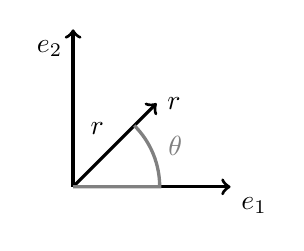
\begin{tikzpicture}[very thick]
        % \draw[fill=gray!30] (0,0)circle(1);
        \draw[->](0,0) --++ (2,0)node[below right ]{$\bm{e}_1$};
        \draw[->](0,0) --++ (0,2)node[below left ]{$\bm{e}_2$};
        \draw[->](0,0) --++ (45:1.5)node[right]{$r$}node[midway, above left]{$r$};
        \draw[gray](0,0) --++ (0:1.1)arc(0:45:1.1)node[below right]{$\;\;\;\theta$};
    \end{tikzpicture}   
	\begin{tikzpicture}[tdplot_main_coords,scale = 0.3]
		\draw[->,thick] (0,0,0) -- (6.5,0,0) node [pos=1.1] {$\bm{e}_1$};
		\draw[->,thick] (0,0,0) -- (0,6,0) node [pos=1.05] {$\bm{e}_2$};
		\draw[->,thick] (0,0,0) -- (0,0,5.5)  node [pos=1.05] {$\bm{e}_3$};   
		\tdplotsetcoord{P'}{7}{\thetavec}{\phivec}
    	\tdplotsetcoord{P''}{1}{90}{90+\phivec}
    	\tdplotsetcoord{P'''}{1}{90+\thetavec}{\phivec}
		\tdplotsetcoord{P}{6}{\thetavec}{\phivec}
		\draw[->] (0,0,0) -- (P) node [midway, above] {$r$};
		\draw[thick] (0,0,0) -- (2,4,0);
		\draw[dashed] (2,4,4) -- (2,4,0);
		\draw[dashed] (2,0,0) -- (2,4,0) node [pos=-0.1] {$x$};
		\draw[dashed] (0,4,0) -- (2,4,0) node [pos=-0.3] {$y$};
		\draw[dashed] (0,0,4) -- (2,4,4) node [pos=-0.1] {$z$};
		\draw[dashed, tdplot_main_coords] (4.47,0,0) arc (0:90:4.47);
		\node[fill=black, circle, inner sep=0.8pt] at (2,4,4) {};
		\tdplotdrawarc{(0,0,0)}{0.7}{0}{\phivec}{below}{$\phi$}
	    \tdplotsetthetaplanecoords{\phivec}
	    \tdplotdrawarc[tdplot_rotated_coords]{(0,0,0)}{0.5}{0}{\thetavec}{}{}
	    \node at (0,0.25,0.67) {$\theta$};
	\end{tikzpicture}

    \caption{Parametrization of the problem for 2D and 3D case.}
    \label{fig:schemeshpere}
\end{figure}
Now let's derive the first 4 moments for a 2D spherical particle. 
The zeroth moment reads as,
\begin{equation}
    \mathcal{G}^0 
    = \int_V  d\bm{y} 
    = \int_0^{2\pi}\int_0^{R}  d\bm{y} 
    = [\theta]_0^{2\pi}[r]_0^{R} 
    = 2\pi R
\end{equation}
where we used the notation depicted on the scheme \ref{fig:schemeshpere}.
The first moment as already mentioned is, $\mathcal{G}^1 = \int \bm{r}_\alpha dV = 0$.
Next, the second moment yields,
\begin{equation}
    (\mathcal{G}^2)_{ij}
    = \int_V r_ir_j d\bm{y} 
    = \int_0^{2\pi}\int_0^{R} r_ir_j d r dr d\theta 
    = \int_0^{R} r^3 dr \int_0^{2\pi} r_ir_j d\theta  
    = \frac{R^4}{4} \int_0^{2\pi} r_ir_j d\theta 
\end{equation}
where $\bm{r} = (\cos{\theta}, \sin{\theta})$. 
Then, 
\begin{equation}
    \mathcal{G}^2 = \frac{R^4}{4}\left[\begin{tabular}{cc}
        $\pi$&$0$\\
        $0$&$\pi$\\
    \end{tabular}
    \right].
\end{equation}
More generally the $l^{th}$ moment reads as, 
\begin{equation}
    (\mathcal{G}^l)_{i_1i_2\ldots i_l}
    = \frac{R^{l+2}}{l+2} \int_0^{2\pi} r_{i_1}r_{i_2}\ldots r_{i_l} d\theta 
\end{equation}
Then, two things can be shown. 
The first one, is that the components off-diagonal of $\mathcal{G}^l$ are null. 
The second, is that the values on the diagonal are the same. 
If we consider the sum on all indices, the product $r_{i_1}r_{i_2}\ldots r_{i_l}$ can be written $(\cos\theta+\sin\theta)^l$.
Moreover, 
\begin{equation}
    (\cos\theta+\sin\theta)^l  = \sum_{k=0}^l\binom{l}{k}\cos^k\theta\sin^{l-k}\theta
\end{equation}
Thus, the integral $\int_0^{2\pi} r_{i_1}r_{i_2}\ldots r_{i_l} d\theta$ always follows this form,
\begin{equation}
    \int_0^{2\pi} \cos^k\theta\sin^{l-k}\theta d\theta \;\;\;\forall k\leq l. 
    \label{eq:cossin}
\end{equation}
Now, we can note that the diagonal components $I$ and $II$ (i.e. the diagonal in the sense that all the indices are the same) are equal to,
\begin{equation}
    (\mathcal{G}^l)_{I}
    = \int_0^{2\pi} \cos^l d\theta\;\;\;
    (\mathcal{G}^l)_{II}
    = \int_0^{2\pi} \sin^l d\theta  
\end{equation}
Let's develop the first term, 
\begin{align*}
    (\mathcal{G}^l)_{I}
    &= \int_0^{2\pi} \cos^l d\theta\\
    &= \frac{1}{l} \left[\cos^{l-1}\theta\sin\theta \right]_0^{2\pi} + \frac{l-1}{l} \int_0^{2\pi} \cos^{l-2} d\theta.\\
\end{align*}
The first term on the right hands side is always null. 
Indeed, $\cos$ is pair at any power of, $l-1$, and $\sin$ is odd, thus the product of the two terms is an odd function. 
Moreover, the product between $\sin$ or $\cos$ are at least $2\pi$ periodic. 
Therefore, the integral taken between $0$ and $\pi$ is null, and the relation reduce to, 
\begin{equation*}
    (\mathcal{G}^l)_{I}
    = \int_0^{2\pi} \cos^l d\theta
    =  \frac{l-1}{l} \int_0^{2\pi} \cos^{l-2} d\theta\\
    =  \frac{l-1}{l}\frac{l-3}{l-2} \int_0^{2\pi} \cos^{l-4} d\theta\\
\end{equation*}
If we keep repeating the process we eventually arrive to the smallest power. 
Which is either $0$ or $1$ if we start by, respectively a number $l$ pair and a number $l$ odd.
Therefore, we pose $l = 2q$ in the first case and $l = 2q+1$ in the second, 
\begin{equation*}
    (\mathcal{G}^{2q})_{I}
    =  \frac{2q-1}{2q}\frac{2q-3}{2q-2} \int_0^{2\pi} \cos^{2q-4}\theta d\theta\\
    =  \prod^{q-1}_{k= 0}\frac{2q-2k-1}{2q-2k} \int_0^{2\pi}  d\theta\\
    =  \prod^{q-1}_{k= 0}\frac{2q-2k-1}{2q-2k} 2\pi\\,
\end{equation*}
and,
\begin{equation*}
    (\mathcal{G}^{2q+1})_{I}
    =  \prod^{q}_{k= 0}\frac{2q-2k}{2q-2k+1} \int_0^{2\pi} \cos \theta d\theta\\
    = 0.
\end{equation*}
Similar calculation can be done for the powers of $\sin$, and it yields the same results. 
Therefore, the diagonal components of the $l^{th}$ order tensor of a disk are, 
\begin{equation}
    \mathcal{G}_{I}^l=\mathcal{G}_{II}^l = \left\{\begin{tabular}{cc}
        $\prod^{q-1}_{k= 0}\frac{2q-2k-1}{2q-2k} 2\pi $& if $l = 2q$     \\
        $0 $        & if $l = 2q+1$
    \end{tabular}\right.
    \label{eq:cosl}
\end{equation}
In fact, if we can carry out similar calculations for the integral, \ref{eq:cossin}, we find that, 
\begin{equation}
    \int_0^{2\pi} \sin^k \cos^{l-k} dV = \frac{1}{2}\frac{k-1}{l-k-1} \int_0^{2\pi} \sin^{l-2}\theta \cos^{l-k+2}\theta d\theta.
\end{equation}
Note that taking $l = 2q$ or $l=2q+1$ leads to either $\sin^0\theta^{l-k+2q} $ or $\sin \theta^{l-k+2q+1}$ in the integral. 
Therefore, the integral of  $\sin \theta^{l-k+2q+1}$ between $0$ and $2\pi$ will ultimately cancel out. 
Therefore, we obtain the following relation in the non-null cases,
\begin{equation}
    \int_0^{2\pi} \sin^k \cos^{l-k} d\theta = \left\{\begin{tabular}{cc}
        $\prod^{q-1}_{n=0}\frac{2q-2n-1}{l-2q+2n+1} \int_0^{2\pi} \cos^{l} d\theta$& if $k = 2q$     \\
        $0 $        & if $l = 2q+1$
    \end{tabular}\right.
\end{equation}
Using \ref{eq:cosl} yields,
\begin{equation}
    \int_0^{2\pi} \sin^k \cos^{l-k} d\theta = \left\{\begin{tabular}{cc}
        $\prod^{q-1}_{n=0}\frac{2q-2n-1}{2r-2q+2n+1} \prod^{r-1}_{n= 0}\frac{2r-2n-1}{2r-2n} 2\pi $& if $k = 2q$ and $l = 2r$    \\
        $0$        & if $k = 2q  $ and $l = 2r +1$\\
        $0$        & if $k = 2q+1$ and $l = 2r$\\
        $0$        & if $k = 2q+1$ and $l = 2r +1$
    \end{tabular}\right.
\end{equation}
The remaining question is now, how to link the indexes of the tensor to the value of $k$.
If we consider a tensor of order $2$ it is easy to say that, 
\begin{equation}
    \mathcal{G}_{ij} = \delta_{ij} \frac{R^4}{4}\pi. 
\end{equation} 
For a $4^{th}$ order tensor it is given by, 
\begin{equation}
    \mathcal{G}_{ijkl} = (\delta_{ij}\delta_{kl} + \delta_{ik}\delta_{lj}) \frac{R^6}{8} \pi
\end{equation} 
we can deduce the pattern for the higher order tensor. 
Indeed, the non-null terms can be defined by the sum of all the possible product of $\delta$.
It can be shown that for a tensor of order $l$ the number of combination of $\delta$ is $n= 1+(l/2-1)l/2$.
}
\section{3D sphere shape tensor}
For spherical particles, it is possible to carry out similar calculation using spherical coordinate. 
Nevertheless, it is more convenient to use tensor calculation for this matter. 
Using spherical coordinates it follows,
\begin{align*}
    \mathcal{G}_{i_1i_2\ldots i_l}^l 
    &= \rho_d \int_{V_\alpha} \prod^l_{m=1}r^\alpha_{i_m} dV\\
    &= \rho_d \int_0^R r^{l+2} dr  
      \int_{S_\alpha} \prod^l_{m=1}r^\alpha_{i_m} dS\\
    &=\rho_d \frac{R^{l+3}}{l+3}
      \int_{S_\alpha}  n_{i_l} \prod^{l-1}_{m=1} r^\alpha_{i_m} dS\\
    &=\rho_d \frac{R^{l+3}}{l+3}
      \int_{V_\alpha}  \partial_{i_l} \left(\prod^{l-1}_{m=1} r^\alpha_{i_m}\right) dV\\
    &=\rho_d \frac{R^{l+3}}{l+3}\sum_{k=1}^{l-1} \delta_{i_l i_k}
      \int_{V_\alpha}  \prod^{l-1}_{\substack{m=1\\ m\neq k}} r^\alpha_{i_m} dV\\
\end{align*}
where we recognize the $l-2$ order shape tensor in the last expression. 
By carrying the same calculation for this tensor we can compute the original $l^{th}$ order shape tensor in a recursive manner. 
We note that all odds order shape tensor will reduce to a sum of $\int r^\alpha dV$ which is null. 
To conclude, the  $l^{th}$ shape tensor of any spherical particles is null for any odd order. 
Moreover, for even order tensor we can note that the components non-null are carried by Kronecker symbols which is the expression of isotropy of the particle. 
Indeed, repeating the previous formula leads to this expression,
\begin{align*}
    \mathcal{G}_{i_1i_2\ldots i_l}^l 
    &=\rho_d \frac{R^{l+3}}{l+3}\sum_{a=1}^{l-1} \delta_{i_l i_a}
      \int_{V_\alpha}  \prod^{l-1}_{\substack{m=1\\ m\neq a}} r^\alpha_{i_m} dV\\
    &=\rho_d \frac{R^{l+3}}{l+3}
    \frac{R^{l+1}}{l+1}\sum_{a=1}^{l-1} \delta_{i_l i_a}
    \sum_{\substack{b=1\\ b\neq a}}^{l-2} \delta_{i_{l-1} i_b}
      \int_{V_\alpha}  \prod^{l-2}_{\substack{m=1\\ m\neq a\\ m\neq b}} r^\alpha_{i_m} dV\\
    &=\rho_d \frac{R^{l+3}}{l+3}
    \frac{R^{l+1}}{l+1} 
    \ldots
    \frac{R^3}{3}
    V_\alpha
    \delta_{i_l i_a}
    \delta_{i_{l-1} i_b}
    \delta_{i_{l-2} i_c}
    \ldots
    \delta_{i_2i_1},
\end{align*}
In further developments we will refer to the product of all the scalar values with the letter $A^l$. 
Therefore, 
\begin{equation}
    \mathcal{G}_{i_1i_2\ldots i_l}^l 
    = A^l V_\alpha
    \delta_{i_l i_a}
    \delta_{i_{l-1} i_b}
    \delta_{i_{l-2} i_c}
    \ldots
    \delta_{i_2i_1},
    \label{eq:shapeT}
\end{equation}
where it is implies that we sum the expression on $a$, $b$, $c\ldots$ in their respective range. 

From this formula we can derive the theoretical expression of the second order shape tensor. 
\begin{equation*}
    \mathcal{G}_{ij} 
    = \rho \int_{V_\alpha} \textbf{r} \textbf{r} dV 
    = \rho \int_0^R r^2 dr \int_{S_\alpha} \textbf{n} \textbf{n}  dS 
    = \rho \frac{R^3}{3} \int_{V_\alpha} \grad \textbf{n} dV
    = \rho \frac{R^2}{3} V_\alpha \delta_{ij}
\end{equation*}
where we have used the relation $\frac{\partial}{\partial y_i}n_j = R^{-1} \delta_{ij}$, note that this is equivalent to the regular calculation, i.e. 
\begin{equation*}
    \mathcal{G}_{zz} 
    = \int_{V_\alpha} r^2 \cos^2{\theta} dV 
    = \int_{0}^R \int_{\phi = 0}^{2\pi} \int_{\theta = 0}^{\pi} r^4 \cos^2{\theta} \sin{\theta} drd\theta d\phi
    = \frac{4R^5}{15}\pi
\end{equation*}

POZRIKIDIS P 217 

\tb{
\subsection{Second order shape tensor for elongated particles}

Now let's consider any particles oriented along its axis of revolution $\bm{p}$. 
Any shape tensor can be expressed as $\mathcal{G}^2_{ij} = p_ip_j G_{||} + (\delta_{ij} - p_ip_j) G_{\bot}$ where $G_\bot$ and $G_{||}$ are constants value corresponding to Eigenvalues values of the shape tensor. 
For antisymmetric particles the Eigenvectors are aligned with the axis of revolution. 
Therefore, using a polar coordinates frame $(r, \theta, z)$ aligned with $\bm{p}$ yields the following formulas for the Eigenvalues of the shape tensor :
\begin{equation}
    G_{||} = \int_V z z dV \;\;\;\;\;\;
    G_{\bot} = \int_V r^2 \cos^2\theta dV.
\end{equation}
As an example let's now consider cylindrical particles of radius $R$ and aspect ratio $\chi$.
Then,
\begin{equation}
    G_{||} = \int_0^R\int_{-\chi R}^{\chi R} \int_0^{2\pi} z z r dr d\theta dz
    = \frac{2}{3}\pi R^5 \chi^3
\end{equation}
\begin{equation}
    G_{\bot} = \int_0^R\int_{-\chi R}^{\chi R} \int_0^{2\pi} r^3 \cos^2\theta dr d\theta dz
    = \frac{1}{2} \pi R^5 \chi.
\end{equation}
If we consider a 2D ellipse where the main axis are of length $a$ and $b$ we can express the shape tensor as,
\begin{equation}
    \mathcal{G}_{11}
    = \frac{\pi}{4}a^3b,
    \;\;\;\; 
    \mathcal{G}_{22}
    = \frac{\pi}{4}b^3a. 
    \label{eq:shapeellipse}
\end{equation}

}
\section{Kinematic equations for the $l^{th}$ order surface tensor.}

Here is the proof of the surface tensor derivations,
\begin{equation*}
    \ddt \int_{S_\alpha} dS 
    = \int_{S_\alpha} \grad_I \cdot \textbf{u}_I dS
\end{equation*}
\begin{equation*}
    \ddt \int_{S_\alpha} \textbf{r} dS 
    = \int_{S_\alpha} \textbf{r} \grad_I \cdot \textbf{u}_I dS
    + \int_{S_\alpha} \textbf{u}_I  \cdot (\textbf{I}-\textbf{nn}) dS
    - \textbf{u}_\alpha \int_{S_\alpha} dS
\end{equation*}
\begin{equation*}
    \ddt \int_{S_\alpha} \textbf{rr} dS 
    = \int_{S_\alpha} \textbf{rr} \grad_I \cdot \textbf{u}_I dS
    + 2 \int_{S_\alpha}\textbf{r} \textbf{u}_I  \cdot (\textbf{I}-\textbf{nn}) dS
    - \int_{S_\alpha} \textbf{u}_\alpha \textbf{r} + \textbf{r}  \textbf{u}_\alpha dS
\end{equation*}
Now we can write the derivation for an arbitrary tensor orders, using the Reynolds transport theorem it reads, 
\begin{align*}
    \ddt \int_{S_\alpha} \pri{1}{n}dS
    &= \int_{S_\alpha} \pddt \left(
        \pri{1}{n}
    \right) dS
    + \int_{S_\alpha} 
    \partial_k^I  \left(
        u^I_k \pri{1}{n}
    \right)dS \\
    &= - \sum_{e=1}^n u^\alpha_{i_e} \int_{S_\alpha} 
        \prod_{\substack{m = 1 \\m \neq e}}^{n} r_{i_m}
     dS
    + \int_{S_\alpha} u^I_k
    \partial_k^I  \left(
         \prod_{m=1}^{n} r_{i_m}
    \right)dS \\
    &+ \int_{S_\alpha} 
    \prod_{m=1}^{n} r_{i_m}
    \partial_k^I u^I_k 
    dS \\
\end{align*}
Using the definition of the surface derivative
\begin{align*}
    \ddt \int_{S_\alpha} \pri{1}{n}dS
    &= \int_{S_\alpha} 
    \prod_{\substack{m = 1 \\m \neq e}}^{n} r_{i_m}
    \partial_k^I u^I_k 
    dS 
    - \sum_{e=1}^n u^\alpha_{i_e} \int_{S_\alpha} 
    \prod_{\substack{m = 1 \\m \neq e}}^{n} r_{i_m}dS \\
    &+ \sum_{e=1}^n \int_{S_\alpha} u^I_k
    \prod_{\substack{m = 1 \\m \neq e}}^{n} r_{i_m}
    (\delta_{ki_e} - n_kn_{i_e}) dS \\
    &= \int_{S_\alpha} 
    \prod_{\substack{m = 1 \\m \neq e}}^{n} r_{i_m}
    \partial_k^I u^I_k dS 
    + \sum_{e=1}^n  \int_{S_\alpha} (w^I_{i_e} - u^I_kn_kn_{i_e}) 
    \prod_{\substack{m = 1 \\m \neq e}}^{n} r_{i_m}dS \\
\end{align*}
Thus, 
\begin{align*}
    \int_{S_\alpha} 
    \prod_{\substack{m = 1 \\m \neq e}}^{n} r_{i_m}
    \partial_k^I u^I_k dS 
    &=
    \ddt \int_{S_\alpha} \pri{1}{n}dS
    + \sum_{e=1}^n u^\alpha_{i_e} \int_{S_\alpha} 
    \prod_{\substack{m = 1 \\m \neq e}}^{n} r_{i_m}dS \\
    &+ \sum_{e=1}^n \int_{S_\alpha} u^I_k
    \prod_{\substack{m = 1 \\m \neq e}}^{n} r_{i_m}
    (n_kn_{i_e} - \delta_{ki_e}) dS \\
\end{align*}


\section{Equations for arbitrary moment of mass.}
Let consider the $l^{th}$ order shape tensor $\mathcal{G}^l_\alpha$ of a given particle $\alpha$. 
In this section we demonstrate how to take the time derivative of any tensor $\mathcal{G}^l_\alpha$. 
In this section we are going to make use of Einstein summation convention to represent the arbitrary order tensors. 
Besides, for a better understanding of the equations we use the notation $\bm{r}^\alpha$ for $\bm{r}_\alpha$ (which is the distance between the center of mass and a given point). 
The shape tensor of any order $l$ is defined by,
\begin{equation}
    \mathcal{G}_{i_1i_2\ldots i_l}^l = \rho_d \int_{V_\alpha} \prod^l_{m=1}r^\alpha_{i_m} dV,
\end{equation}
where each $i_m$ represent different indices. 
Then taking the time derivative and using \ref{eq:timetransport} gives the following relation,
\begin{multline}
    \frac{d}{dt}\mathcal{G}_{i_1i_2\ldots i_l}^l 
    = \rho_d \int_{V_\alpha} \left[ \frac{\partial}{\partial t} \left(\prod^l_{m=1}r^\alpha_{i_m}\right) 
    + \frac{\partial}{\partial y_k} \left(u_k\prod^l_{m=1}r^\alpha_{i_m}\right) \right]dV\\
    +\int_{S_\alpha} \prod^l_{m=1}r^\alpha_{i_m} \rho_d \left((u_I)_k - u_k\right) n_k^\alpha dS,
\end{multline}
where we recall that the second term is due to mass transfer and will be noted $T^l_\alpha$ for compactness. 
Using, the product rule on the derivative yields the following relation :
\begin{multline}
    \frac{d}{dt}\mathcal{G}_{i_1i_2\ldots i_l}^l 
    = \rho_d \int_{V_\alpha} \sum_{e=1}^l \left[ \prod^l_{\substack{ m=1 \\   m \neq e}}r^\alpha_{i_m} \frac{\partial}{\partial t} \left(r_{i_e}\right) 
    + \prod^l_{m=1}r^\alpha_{i_m} \frac{\partial}{\partial y_k} \left(u_k\right) 
    \right.\\
    \left.
    + u_k \frac{\partial}{\partial y_k} \left(\prod^l_{m=1}r^\alpha_{i_m}\right) \right]dV
    +T^\alpha_{i_1i_2\ldots i_l},
\end{multline}
where we can recognize the second term as the divergence of the velocity, which is null since the fluid is incompressible. 
Now, by making use of the product rule on the third term it yields,
\begin{equation}
    \frac{d}{dt}\mathcal{G}_{i_1i_2\ldots i_l}^l 
    = \rho_d \int_{V_\alpha} \sum_{e=1}^l \prod^l_{\substack{ m=1 \\   m \neq e}} r^\alpha_{i_m}\left[ \frac{\partial}{\partial t} \left(r_{i_e}\right) 
    + u_k \frac{\partial}{\partial y_k} \left(r_{i_e}\right) \right]dV
    +T^\alpha_{i_1i_2\ldots i_l},
\end{equation}
The term within the brackets can be simplified thanks to \ref{eq:momentofmomentumDev} as the fluctuation of the velocity around the center of mass noted $\bm{w}^\alpha$.
\begin{equation}
    \frac{d}{dt}\mathcal{G}_{i_1i_2\ldots i_l}^l 
    = \rho_d \sum_{e=1}^l \int_{V_\alpha}  \prod^l_{\substack{ m=1 \\   m \neq e}} r^\alpha_{i_m} w_{i_e}dV
    +T^\alpha_{i_1i_2\ldots i_l}.
\end{equation}
In the summation sign we can recognize the $(l-1)^{th}$ moment of momentum tensor. 
\begin{equation}
    \frac{d}{dt}\mathcal{G}_{i_1i_2\ldots i_l}^l 
    = \sum_{e=1}^l P^\alpha_{i_1\ldots i_e\ldots i_l}
    +T^\alpha_{i_1i_2\ldots i_l}.
\end{equation}
Each terms in the sum is just the same tensor where we have permuted the indices. 
All the possible permutations are in the sum since there is only two different vectors, i.e. $\bm{r}^\alpha$ and $\bm{w}^\alpha$, and $\bm{w}^\alpha$ takes all the places among the $\bm{r}^\alpha$.
Furthermore, the sum of all the permutations of a tensor is proportional to its symmetric part \citep{itin2022decomposition}. 
Thus, we define the $^\text{Sym}$ operator which return the symmetric part of any $l^{th}$ order tensor. 
In tensor form the previous relation is then,
\begin{equation}
    \frac{d}{dt}\mathcal{G}^l 
    = l (\bm{P}_\alpha^l)^{\text{Sym}}
    +\bm{T}^\alpha.
    \label{eq:dt_G_alpha_l}
\end{equation}
The rate of change of the shape of the particle is therefore linked directly to its own moment of momentum. 
But it does not depend on the antisymmetric part. 
Which mean that the angular momentum do not play any role in the change of the shape. 
Next, we apply the particular average to this set of equations using \ref{eq:partia}.
It yields a $l$ order equation, 
\begin{equation}
    \partial_t\left(n\left<\mathcal{G}_{i_1i_2\ldots i_l}^l\right>^p\right) 
    +\partial_k\left(n\left<u_k\mathcal{G}_{i_1i_2\ldots i_l}^l\right>^p\right) 
    = n\;l\left<(P^\alpha_{i_1\ldots i_e\ldots i_l})^\text{Sym}\right>
    +n\left<T^\alpha_{i_1i_2\ldots i_l}\right>.
\end{equation}
Then, we obtained a set of $l$ equations which describe the evolution and the transport of the averaged shape properties. 
In the following we review the meaning for each of the first orders equations. 
Besides, we neglect the mass transfer term as it is not useful for our application. 
\tb{In those equations we must add the conservation of volume condition.
Look into \citet{maffettone1998equation}}

\tb{
\subsection{Equation at the first order}
At the first order we have the following relation, 
\begin{equation}
    \frac{d}{dt}\mathcal{G}^1 
    =  \frac{\partial}{\partial t} \rho_d \int_{V_\alpha} \bm{r}_\alpha dV 
    = \rho_d \int_{V_\alpha} \bm{w}_\alpha dV
    = 0. 
\end{equation}
We recall that $\bm{r}_\alpha$ is defined such that $\int_{V_\alpha} \bm{r}_\alpha dV$ is null. 
Therefore, this relation leads to a null term. 

\subsection{Second order relation}
At the second order the relation is, 
\begin{equation}
    \frac{d}{dt}\mathcal{G}^2
    = 2 (\bm{P}_\alpha^2)^{\text{Sym}}. 
    \label{eq:dGdt}
\end{equation}
Therefore the following calculation might not make sense
Thus, the rate of change of the shape of the particle is equal to the symmetric part of the moment of momentum. 
Let's study this equation in the linear displacement hypothesis to get a more physical conclusion of the matter. 
From the previous section (\ref{eq:linear2}), and by keeping only the symmetric part of $\bm{P_\alpha}$ one can deduce, 
\begin{equation}
    \frac{d}{dt}\mathcal{G}^2
    = 2 \bm{E}_\alpha \cdot \mathcal{G}^2. 
\end{equation}
Which gives us a set of $d^2$ (where $d$ is the dimension) linear differential equations for the shape tensor, namely
\begin{equation}
    \frac{d}{dt}\mathcal{G}^2_{ij}
    = 2 E^\alpha_{ik}  \mathcal{G}^2_{kj}. 
\end{equation}


}
\section{Dynamical equations for the $l^{th}$ order momentum tensor.}
Let consider the $l^{th}$ order momentum tensor $\bm{P}^l_\alpha$ of a given particle $\alpha$. 
In this section we demonstrate how to take the time derivative of any tensor $\bm{P}^l_\alpha$. 
We are going to make use of Einstein summation convention to represent the arbitrary order tensors. 
The momentum tensor of any order $l$ is defined by,
\begin{equation}
    P_{i_1i_2\ldots i_l}^{l} = \rho_d \int_{V_\alpha} \prod^{l-1}_{m=1}r^\alpha_{i_m} u_{i_l} dV,
\end{equation}
Then taking the time derivative and using \ref{eq:timetransport} gives the following relation,
\begin{multline*}
    \frac{d}{dt}P_{i_1i_2\ldots i_l}^l 
    = \rho_d \int_{V_\alpha} \left[ \frac{\partial}{\partial t} \left(\prod^{l-1}_{m=1}r^\alpha_{i_m} u_{i_l}\right) 
    + \frac{\partial}{\partial y_k} \left(u_k\prod^{l-1}_{m=1}r^\alpha_{i_m} u_{i_l}\right) \right]dV\\
    +\int_{S_\alpha} \prod^{l-1}_{m=1}r^\alpha_{i_m} u_{i_l} \left((u_I)_k - u_k\right) n_k^\alpha dS.
\end{multline*}
The last term is the moment of momentum of mass transfer and will be referred as $(T_u^\alpha)_{i_1i_2\ldots i_l}$ 
using the product rule for the derivation of the terms inside the first integral gives, 
\begin{multline*}
    \frac{d}{dt}P_{i_1i_2\ldots i_l}^l 
    = 
    \rho_d \int_{V_\alpha} u_{i_l}\left[  \frac{\partial}{\partial t} \left(\prod^{l-1}_{m=1}r^\alpha_{i_m} \right) 
    + u_k \frac{\partial}{\partial y_k} \left(\prod^{l-1}_{m=1}r^\alpha_{i_m}\right) \right]dV\\
    +\rho_d \int_{V_\alpha}  \prod^{l-1}_{m=1}r^\alpha_{i_m} \left[ 
    \frac{\partial}{\partial t} \left(u_{i_l}\right) 
    + \frac{\partial}{\partial y_k} \left(u_k u_{i_l}\right) 
    \right]dV
    +(T_u^\alpha)_{i_1i_2\ldots i_l},
\end{multline*}
Using the same calculation as in the previous section for the first term, and using,  the development carried in \ref{chap:avg} for the second leads to, 
\begin{multline*}
    \frac{d}{dt}P_{i_1i_2\ldots i_l}^l 
    = 
    \rho_d \sum_{e=1}^{l-1} \int_{V_\alpha} u_{i_l}  \prod^{l-1}_{\substack{ m=1 \\   m \neq e}} r^\alpha_{i_m} w_{i_e}dV\\
    +\rho_d \int_{V_\alpha}  \prod^{l-1}_{m=1}r^\alpha_{i_m} \left[ 
    \partial_k \sigma_{ki_l} + b_{i_l} + f^\sigma_{i_l}   
    \right]dV
    +(T_u^\alpha)_{i_1i_2\ldots i_l}.
    \label{eq:B68}
\end{multline*}
Besides, we can derive the following relation,
\begin{multline*}
    \partial_k\left(\prod^{l-1}_{m=1}r^\alpha_{i_m}  \sigma_{ki_l}\right)
    = \prod^{l-1}_{m=1}r^\alpha_{i_m} \partial_k \sigma_{ki_l} 
    + \sigma_{ki_l} \partial_k \prod^{l-1}_{m=1}r^\alpha_{i_m}\\
    = \prod^{l-1}_{m=1}r^\alpha_{i_m} \partial_k \sigma_{ki_l} 
    + \sum^{l-1}_{e =1} \sigma_{i_ei_l} \prod^{l-1}_{\substack{m=1\\ m\neq e}}r^\alpha_{i_m}  
\end{multline*}
Therefore, term involving the divergence of the stress in \ref{eq:B68} can be rewritten as so, 
\begin{equation}
    \int_{V_\alpha} \prod^{l-1}_{m=1}r^\alpha_{i_m} \partial_k \sigma_{ki_l} dV
    =
    \int_{V_\alpha} \partial_k\left(\prod^{l-1}_{m=1}r^\alpha_{i_m}  \sigma_{ki_l}\right) dV 
    -\int_{V_\alpha} \sum^{l-1}_{e=1} \sigma_{i_ei_l}  \prod^{l-1}_{\substack{m=1\\ m\neq e}}r^\alpha_{i_m}  dV
\end{equation}
Using the divergence theorem on the first term yields,  
\begin{equation}
    \int_{V_\alpha} \prod^{l-1}_{m=1}r^\alpha_{i_m} \partial_k \sigma_{ki_l} dV
    =
    \int_{S_\alpha} \prod^{l-1}_{m=1}r^\alpha_{i_m}  \sigma_{ki_l}^fn_k dS 
    -\int_{V_\alpha} \sum^{l-1}_{e=1} \prod^{l-1}_{\substack{m=1\\ m\neq e}}r^\alpha_{i_m}  \sigma_{i_ei_l}^d dV,
\end{equation}
noticing that the first term represent the $l^h$ order of the hydrodynamic moment and the terms in brackets in \ref{eq:B68} represent the $l^{th}$ moment of the body forces and surface tension force,
\begin{multline}
    \frac{d}{dt}P_{i_1i_2\ldots i_l}^\alpha
    = 
    (M^h_\alpha)_{i_1\ldots i_l}
    +(M^\sigma_\alpha)_{i_1\ldots i_l}
    +(M^b_\alpha)_{i_1\ldots i_l}\\
    +\rho_d  \int_{V_\alpha} \sum_{e=1}^{l-1}  \prod^{l-1}_{\substack{ m=1 \\   m \neq e}} r^\alpha_{i_m} w_{i_e} u_{i_l}dV
    -\rho_d\int_{V_\alpha} \sum^{l-1}_{e=1} \prod^{l-1}_{\substack{m=1\\ m\neq e}}r^\alpha_{i_m}  \sigma_{i_ei_l}^d dV
    +(T_u^\alpha)_{i_1i_2\ldots i_l}.
    \label{eq:dt_P_order_l}
\end{multline}
Furthermore, as a consequence of the summation, the $5^{th}$ term on the right hands side is symmetric on all indices from $1$ to $l-1$.
Besides, the stress tensor is by definition symmetric on its own indices, i.e. $i_e$ and $i_l$. Therefore, this term is symmetric on all its indices and will vanish if one takes the antisymmetric part of the equation. 
By applying the decomposition of the velocity $u_i = u^\alpha_i + w_i$ we obtain a fully symmetric tensor plus the moments of the fluctuations times the mean velocity.
Knowing that it is possible to derive two distinct equations, one for the antisymmetric part and symmetric part. 
Using \ref{eq:Gorderl} the equation for the symmetric part reads as,
\begin{multline*}
    \frac{d^2}{dt^2}G_{i_1i_2\ldots i_l}^\alpha
    = 
    (S^h_\alpha)_{i_1\ldots i_l}
    +(S^\sigma_\alpha)_{i_1\ldots i_l}
    +(S^b_\alpha)_{i_1\ldots i_l}\\
    +\rho_d  \int_{V_\alpha} \sum_{e=1}^{l-1}  \prod^{l-1}_{\substack{ m=1 \\   m \neq e}} r^\alpha_{i_m} w_{i_e} u_{i_l}dV
    -\rho_d\int_{V_\alpha} \sum^{l-1}_{e=1} \prod^{l-1}_{\substack{m=1\\ m\neq e}}r^\alpha_{i_m}  \sigma_{i_ei_l}^d dV
    +(T_u^\alpha)_{i_1i_2\ldots i_l}.
\end{multline*}
Which is the equation of state of the particle shape tensor. 
And the antisymmetric part yields, 
\begin{multline*}
    \frac{d^2}{dt^2}G_{i_1i_2\ldots i_l}^\alpha
    = 
    (S^h_\alpha)_{i_1\ldots i_l}
    +(S^\sigma_\alpha)_{i_1\ldots i_l}
    +(S^b_\alpha)_{i_1\ldots i_l}\\
    +\rho_d  \int_{V_\alpha} \sum_{e=1}^{l-1}  \prod^{l-1}_{\substack{ m=1 \\   m \neq e}} r^\alpha_{i_m} w_{i_e} u_{i_l}dV
    -\rho_d\int_{V_\alpha} \sum^{l-1}_{e=1} \prod^{l-1}_{\substack{m=1\\ m\neq e}}r^\alpha_{i_m}  \sigma_{i_ei_l}^d dV
    +(T_u^\alpha)_{i_1i_2\ldots i_l}.
\end{multline*}

Anyhow, it is now possible ti apply the particular average the transport of momentum equation yielding, 
\begin{multline*}
    \partial_t\left(n\left<\mathcal{P}_{i_1i_2\ldots i_l}^\alpha\right>^p\right)
    +\partial_k\left(n\left<u_k\mathcal{P}_{i_1i_2\ldots i_l}^\alpha\right>^p\right)
    =
    \pavg{M^\alpha_{i_1\ldots i_l}}\\
    +\rho_d \pavg{ \int_{V_\alpha} \sum_{e=1}^{l-1}  \prod^{l-1}_{\substack{ m=1 \\   m \neq e}} r^\alpha_{i_m} w_{i_e} u_{i_l}dV}
    -\rho_d \pavg{\int_{V_\alpha} \sum^{l-1}_{e=1} \prod^{l-1}_{\substack{m=1\\ m\neq e}}r^\alpha_{i_m}  \sigma_{i_ei_l}^d dV}\\
    + \pavg{T^\alpha_{i_1i_2\ldots i_l}},
\end{multline*}
for the moment of momentum, were
$M^\alpha_{i_1\ldots i_l}$ is the sum of the moments due to the hydrodynamic forces, the surface tension forces and the body forces.

\subsection*{Arbitrary order moments equation}

Let's define the arbitrary moment of the tensor $f$, by, 
\begin{equation*}
    Q_{i_1\ldots i_n}
    = \int_{V_\alpha} 
    \pri{1}{n} f dV
\end{equation*}
Then,
\begin{multline*}
    \ddt Q_{i_1\ldots i_n}
    =\int_{V_\alpha} \left[ \partial_t \left(\pri{1}{n}f\right) 
    + \partial_k \left(u_k \pri{1}{n}f\right) \right]dV\\
    +\int_{S_\alpha} \pri{1}{n} f \left(u^I_k - u_k\right) n_k dS.
\end{multline*}
Using the product rule on the derivatives yields, 
\begin{multline*}
    \ddt Q_{i_1\ldots i_n}
    =\int_{V_\alpha} f \left[ \partial_t \left(\pri{1}{n}\right) 
    + u_k \partial_k \left( \pri{1}{n}\right) \right]dV\\
    +\int_{V_\alpha} \pri{1}{n} \left[ \partial_t \left(f\right) 
    +  \partial_k \left(u_k f \right) \right]dV\\
    +\int_{S_\alpha} \pri{1}{n} f \left(u^I_k - u_k\right) n_k dS.
\end{multline*}
From similar arguments as before one can easily show that, 
\begin{multline*}
    \ddt Q_{i_1\ldots i_n}
    = \sum_{e=1}^{n} \int_{V_\alpha} f  \prod^{n}_{\substack{ m=1 \\   m \neq e}} r_{i_m} w_{i_e}dV
    +\int_{V_\alpha} \pri{1}{n} \grad\cdot\mathbf{\Phi} dV\\
    + \int_{V_\alpha} \pri{1}{n} \textbf{S} dV
    +\int_{S_\alpha} \pri{1}{n} f \left(u^I_k - u_k\right) n_k dS.
\end{multline*}
The second term can be reformulated such as,
\begin{align*}
    \int_{V_\alpha} \pri{1}{n} \grad\cdot\mathbf{\Phi} dV
    &= \int_{S_\alpha} \grad \cdot \left(\pri{1}{n} \mathbf{\Phi} \right)dV
    - \int_{V_\alpha} \mathbf{\Phi} \cdot \grad \left(\pri{1}{n} \right)dV\\
    &= \int_{S_\alpha} \pri{1}{n} \mathbf{\Phi} \cdot \textbf{n}dS
    -\sum_{e=1}^{n} \int_{V_\alpha} \mathbf{\Phi}  \prod^{n}_{\substack{ m=1 \\m \neq e}} r_{i_m}  dV
\end{align*}
Including this relation into the former equation yields, 
\begin{multline*}
    \ddt Q_{i_1\ldots i_n}
    = \sum_{e=1}^{n} \int_{V_\alpha} \prod^{n}_{\substack{ m=1 \\   m \neq e}} r_{i_m} (w_{i_e}f  - \Phi)dV
    +\int_{S_\alpha} \pri{1}{n} \mathbf{\Phi} \cdot \textbf{n}dS\\
    + \int_{V_\alpha} \pri{1}{n} \textbf{S} dV
    +\int_{S_\alpha} \pri{1}{n} f \left(u^I_k - u_k\right) n_k dS.
\end{multline*}
Then it is possible from this equation to carry out a particular average but also to get the local scale equations. 
Indeed, if we consider $V_\alpha$ as being a fixed control volume the above equality can be rewritten such as, 
\begin{multline*}
    \pddt \left(\pri{1}{n}f\right)
    + \grad \cdot \left(\pri{1}{n}f \textbf{u}\right)
    = n  \pri{1}{n-1}  (w_{i_n}f  - \Phi)\\
    + \pri{1}{n} \textbf{S} 
    + \grad \cdot \left( \pri{1}{n} \mathbf{\Phi} \right)
    \label{ap:eq:dt_rrf}
\end{multline*}


\subsection{On the first hydrodynamic moment and its contribution.}

While providing closure term for the first moment the user must know which part is function of the local pressure since it is absolute. 
We recall that the first hydrodynamic moment of a particle reads as,
\begin{equation}
    (M^h_\alpha)_{ij} 
    = \int_{S_\alpha} r^\alpha_i \sigma_{jk} n_k dS.
\end{equation}
In this section we discuss the different contribution from the viscous and pressure stress to the first moment tensor by investigating the specific case of a particle in a uniform flow. 
We consider a flow where pressure can be express as the sum of a constant pressure $p_0$, a constant gradient along the $z$ coordinate, and a fluctuation part $p'$, thus $p =p_0 + f_b z + p'$ where $p'$ is the fluctuation and $f_b$ the constant gradient ($f_b = \rho_f g$ is the case of buoyant flows). 
Therefore, the stress tensor reads as, $\sigma_{jk} = -p \delta_{jk} + \mu_f (\partial_j u_k+\partial_k u_j)$.
Besides, the particles are assumed spherical, thus $r_i = n_i R$ over the surface $S_\alpha$, where $R$ is the radius. 
Injecting the previous facts in the first moment expression gives,
\begin{equation}
    (M^h_\alpha)_{ij} 
    = - p_0 \int_{S_\alpha} r_i n_j dS
    - f_b \int_{S_\alpha} r_i n_j z dS
    - \int_{S_\alpha} r_i n_j p' dS
    + \int_{S_\alpha} r_i n_k \mu_f (\partial_j u_k+\partial_k u_j) dS
    \label{eq:Fistmomentdec}
\end{equation}
The viscous and pressure fluctuation part are function of local property of the flow, 
consequently they cannot be computed theoretically. 
So, let's focus on the first and second terms in the case of spherical particles. 
Using spherical coordinate, any point, $\bm{r} = (r\sin\theta \cos\phi,\; r\sin\theta \sin\phi,\; r\cos\theta )$,
Therefore the first term can be written, 
\begin{equation}
    p_0 \int_{S_\alpha} r_i n_j dS
    = p_0 R^3 \int_{0}^{2\pi}\int_{0}^\pi n_i n_j \sin\theta d\theta d\phi.
\end{equation}
Then, we have to compute the integral of each member of the following matrix,
\begin{multline}
    p_0 R^3 \int_{0}^{2\pi}\int_{0}^\pi n_i n_j \sin\theta d\theta d\phi
    =\\
     p_0 R^3 \int_{0}^{2\pi}\int_{0}^\pi
    \left[
        \begin{matrix}
            \sin^3\theta \cos^2\phi & \sin^3\theta  \cos\phi \sin\phi
            &\cos\theta\sin^2\theta \cos\phi\\
            \sim& \sin^3\theta \sin^2\phi & \sin^2\theta \cos\theta\sin\phi \\
            \sim& \sim & \sin\theta \cos^2\theta \\
        \end{matrix}
    \right]
    d\theta d\phi,
\end{multline}
by using the separation of variable method one can compute any of these integrals and find that only the diagonal components remain, and we find that, 
\begin{equation}
    p_0 R^3 \int_{0}^{2\pi}\int_{0}^\pi n_i n_j \sin\theta d\theta d\phi
    = \frac{4}{3}  p_0 R^3 \pi \delta_{ij}.
\end{equation}
Likewise, the second term of \ref{eq:Fistmomentdec} reads as,
\begin{multline}
    f_b \int_{S_\alpha} r_i n_j z dS
    =\\
     f_b R^3 \int_{0}^{2\pi}\int_{0}^\pi
    \left[
        \begin{matrix}
            \sin^3\theta \cos\theta \cos^2\phi & \sin^3\theta \cos\theta \cos\phi \sin\phi
            &\cos^2\theta\sin^2\theta \cos\phi\\
            \sim& \sin^3\theta \cos\theta \sin^2\phi & \sin^2\theta \cos^2\theta\sin\phi \\
            \sim& \sim & \sin\theta \cos^3\theta \\
        \end{matrix}
    \right]
    d\theta d\phi,
\end{multline}
Since the function depending on $\theta$ are antisymmetric around $\pi/2$ the integrals of the diagonal term are null.
In addition, the anti-diagonal components must be null due to the anisotropy of the geometry, and they are.  
In conclusion, the absolute pressure contribute to the first moment as $ \frac{4}{3}  p_0 R^4 \pi \delta_{ij}$, and the pressure gradient do not. 
Consequently, care must be taken while computing the stresslet on DNS software since we do not want the absolute pressure to appear in the results. 


\subsection{On the first moment of the surface tension}
The aim of this part is to express the link between the first order moment of the surface tension, i.e. $\bm{M}^\sigma_\alpha$ to the shape of the particle, i.e. the shape tensor $\mathcal{G}_\alpha$.
In the moment of momentum equation we see appear the unique contribution to the surface tension on the averaged equation though the first moment of the surface tension defined as,
\begin{equation}
    (M^\sigma_\alpha)_{ij}=\int_{S_\alpha}r^\alpha_i f^\sigma_j dS
\end{equation}
using the definition of the surface forces with a constant surface tension $\sigma$ gives, 
\begin{equation}
    (M^\sigma_\alpha)_{ij}=\int_{S_\alpha}r^\alpha_i \sigma \kappa n_j dS
\end{equation}
where $\kappa = -\nabla \cdot \bm{n}$ is the curvature of the surface. 
For spherical particles $\kappa = 1/R$ where $R$ is the radius of the sphere.
Therefore, the moment over the surface of the particle reads,
\begin{align}
    (M^\sigma_\alpha)_{ij}
    &= \frac{\sigma}{R}\int_{S_\alpha}r^\alpha_i n_j dS
    = \frac{\sigma}{R}\int_{V_\alpha} \partial_j r^\alpha_i dV
    = V_\alpha \frac{\sigma}{R}  \delta_{ij}\\
    &
    = \frac{4}{3} \pi R^2 \sigma  \delta_{ij} 
    \text{ for sphere, and  } 
    \pi R \sigma  \delta_{ij} 
    \text{ for circle.} 
    )
    \label{eq:MtensionCric}
\end{align}
The moment is fully isotropic, and in the static isolated case, it clearly expresses the hydrostatic pressure due to surface force applied on a spherical particle. 

For arbitrary shaped particles it gives we need to decompose the problem in two sub-problems. 
Any geometry can be decomposed by a static sphere of radius $R_m(t)$ plus a perturbed shape which can be described with a $2\pi$ periodic function $f(t,\theta,\phi)$. 
Similarly, we can define the curvature $\kappa$ as the sum of $\kappa_1$, which is the mean curvature and $\kappa_2$ is the fluctuations from the surface of the spherical geometry. Then,
\begin{equation}
    (M^\sigma_\alpha)_{ij}
    =\int_{S_\alpha}r^\alpha_i \sigma \kappa_1 n_j dS
    +\int_{S_\alpha}r^\alpha_i \sigma \kappa_2 n_j dS\\
    = \underbrace{\frac{4}{3} \pi \sigma R_m^2(t)  \delta_{ij}}_{\text{Spherical}}
    +
    \underbrace{\int_{S_\alpha(t)}r^\alpha_i \sigma \kappa_2 n_j dS}_{\text{Deviatoric}},
\end{equation}
where we can clearly identify the spherical and deviatoric part of the moment due to surface forces,
and we empathize the dependency of the surface $S_\alpha(t)$ with time. 
Before going further it is important to note that the deviatoric part of this tensor isn't necessarily symmetric, consequently it must appear in the torque equation.
Now we let's consider a 2D deformable ellipsoid of volume, $\pi R_m^2$, and as semi-minor axis $a(t)$ and $b(t)$. 
By exploiting the conservation of volume property we obtain the following relation, 
$a(t) = R^2_m/b(t)$. 
The coordinates an ellipse can be represented by $\bm{r} = (a(t) \cos\theta, b(t)\sin\theta)$. 
Besides, in 2D it can be shown (see \citet{tryggvason2011direct}) that the normal and curvature of the surface, respectively $\bm{n}$ and $\kappa$ can be express as,
\begin{equation}
    \bm{n} 
    = \frac{\left(b(t) \cos\theta, a(t)\sin\theta\right)}{(a^2(t)\sin^2\theta+b^2(t)\cos^2\theta)^{1/2}},
    \;\;\;\;
    \kappa
    = \frac{- R_m^2}{(a^2(t)\sin^2\theta+b^2(t)\cos^2\theta)^{3/2}}.
\end{equation}

Subsequently, we can formulate $\bm{r}$ as 
$r_i = A_{ik} n_k (a^2(t)\sin^2\theta+b^2(t)\cos^2\theta)^{1/2}$, 
where $A_{ik} =b(t)/a(t) e^1_ie^1_k+a(t)/b(t)e^2_ie^2_k$,
as well, the norm of $|\bm{r}| = (a^2(t)\cos^2\theta+b^2(t)\sin^2\theta)^{1/2}$.
We can now express the first moment of the surface tension in polar coordinate, using the relation 
$dS = (a^2(t)\sin^2\theta+b^2(t)\cos^2\theta)^{1/2}d\theta$.
\begin{equation*}
    (M_{\alpha}^\sigma)_{ij} 
    = - \sigma R_m^2 A_{ik} b(t)^{-3}\int_{0}^{2\pi}
    e_k  e_j 
    (c(t)\sin^2\theta+\cos^2\theta)^{-3/2} 
    d\theta,
\end{equation*}
where $c = b^2/a^2$, $\bm{e}$ is $\bm{n}$ times its own norm, so it can be expressed in terms of $c(t) $ as well. 
It can be demonstrated that the anti-diagonal components are antisymmetric functions, thereby, they vanish under the integration operator $\int_0^{2\pi}$. 
Nonetheless, the integral of the diagonal components are not trivial, indeed they involve elliptical integral of the first and second kind, namely $K(x)$ and $E(x)$. It reads,
\begin{equation*}
    \bm{M}_{\alpha}^\sigma
    = - \sigma R_m^2 A_{ik} \left[    
        \begin{matrix}
            b^{-1} \frac{(E(1 - c^2) - K(1 - c^2))}{c^2-1} & 0\\
            0 & a^{-1} c\frac{cK(1 - c^2) - E(1 - c^2)}{c^2-1}\\
        \end{matrix}
    \right].
\end{equation*}
In the limit of small $(c-1)$ and discarding the terms above $\mathcal{O}(c-1)^2$, the elliptic integral reads,
\begin{align*}
    (\bm{M}_{\alpha}^\sigma)_{22}
    &= - \sigma \pi R_m^2 
            a^{-1} (1 -\frac{3}{4}   (c-1)+\frac{9}{16}   (c-1)^2 )
    +O\left((c-1)^3\right)\\
    (\bm{M}_{\alpha}^\sigma)_{22}
    &= - \sigma \pi R_m^2 
            b^{-1} (1 +\frac{3}{4}   (c-1)-\frac{3}{16}   (c-1)^2)
    +O\left((c-1)^3\right)\\
    \label{eq:momentSigma}
\end{align*}
One can note that for $a(t) = R_m$ we recover the expression for circular drop \ref{eq:MtensionCric}.
\tb{make appear the shape tensor inside}

\subsubsection*{Ellipsoid}

In indices notation,  
\begin{equation*}
    \sigma_{I,ij}^0 =\gamma\left[
    \delta_{ij} - \frac{ H_{ik} H_{jl} :  r_kr_l}{  H_{ab}  H_{ac} r_br_c} \right]
\end{equation*}
Integrating this over a surface will eventually leads to an elliptic integral due to the elliptical surface. 

If the spheroid is aligned with the principal axes $\textbf{H} = \textbf{e}_1\textbf{e}_1 / a^2(t) + (\textbf{e}_2\textbf{e}_2+ \textbf{e}_3\textbf{e}_3)/b^2(t)$.
Thus, $\textbf{H}\cdot \textbf{r} = H_{ij} r_j = {e}_{1,i}{e}_{1,j}r_j / a^2(t) + ({e}_{2,i}{e}_{2,j} + {e}_{3,i}{e}_{3,j})r_j/b^2(t) $ which gives, the vector, 
$\textbf{H}\cdot \textbf{r} = \textbf{e}_{1} x/ a^2(t) + (\textbf{e}_{2}y + \textbf{e}_{3}z)/b^2(t)  = \textbf{e}_i r_i /a_i^2$
Consequently, the second term of the last equality reads in a main axis as, 
\begin{equation*}
    \frac{ H_{ik} H_{jl} :  r_kr_l}{  H_{ab}  H_{ac} r_br_c} 
    = \textbf{e}_i \textbf{e}_j \frac{ r_i r_j /(a_i a_j)^2 }
    {\frac{z^2}{a^4}+\frac{y^2+x^2}{b^4}}
\end{equation*}
To dealt with this ellipsoid integral we may employ the following change of variable :
\begin{align*}
    x = b \sin \theta \cos \phi\\
    y = b \sin \theta \sin \phi\\
    z = a \cos \theta 
\end{align*}
with $\theta \in [0,\pi]$ and $\phi \in [0,2\pi]$. 
The point on the ellipsoid surface can then be written as $\textbf{v} = [x(\theta,\phi),y(\theta,\phi),z(\theta,\phi)]$. 
Now let's first consider the surface calculation, in our coordinate system we have, 
\begin{equation*}
    \iint_S dS
    = 
    \int_{0}^{2\pi}
    \int_{0}^{\pi}
    \left|\frac{\partial \textbf{v}}{\partial \theta} 
    \times 
    \frac{\partial \textbf{v}}{\partial \phi} \right|
    d\theta
    d\phi
\end{equation*}
The partial derivative reads, 
\begin{align*}
    \frac{\partial \textbf{v}}{\partial \theta}
    = 
    b \cos \theta \cos \phi \textbf{e}_x
    + b \cos \theta \sin \phi\textbf{e}_y
    - a \sin \theta \textbf{e}_z
    \\
    \frac{\partial \textbf{v}}{\partial \phi}
    = 
    - b \sin \theta \sin \phi \textbf{e}_x
    + b \sin \theta \cos \phi\textbf{e}_y
\end{align*}
Taking the norm of the above vector cross product yields the relation : 
$dS = \left|\frac{\partial \textbf{v}}{\partial \theta} 
\times 
\frac{\partial \textbf{v}}{\partial \phi} \right| d\theta d\phi = b \sin\theta (a^2\sin^2\theta+ b^2 \cos^2\theta)^{1/2}d\theta d\phi$. 

Injecting these coordinate into the previous integrand formula for the dyadic normal reads, 
\begin{equation*}
    \frac{ H_{ik} H_{jl} :  r_kr_l}{  H_{ab}  H_{ac} r_br_c} 
    = \textbf{e}_i \textbf{e}_j \frac{ r_i r_j /(a_i a_j)^2 }
    {\frac{1}{a^2}\cos^2 \theta+\frac{1}{b^2}\sin^2 \theta (\cos^2 \phi+ \sin^2 \phi)}
    = \textbf{e}_i \textbf{e}_j \frac{ r_i r_j}
    {\frac{(a_i a_j)^2}{a^2}\cos^2 \theta+\frac{(a_i a_j)^2}{b^2}\sin^2 \theta }
\end{equation*}
Due to symmetry consideration the crossed terms are all null thus the remaining terms to evaluate are just the diagonal terms. 
The first term of the surface stress, that we call $S_1$ is the surface energy, i.e. the surface of the ellipsoid times the surface tension coefficient $\gamma$. 
\begin{equation*}
    (S_1)_{ij} 
    = \delta_{ij} 2\pi 
    \int_0^\pi 
    b \sin\theta (a^2\sin^2\theta+ b^2 \cos^2\theta)^{1/2} d\theta 
    = 2\pi b \left[\frac{a^2}{\sqrt{b^2-a^2}} \text{asinh}\left(\frac{\sqrt{b^2-a^2}}{a}\right)+b\right]
\end{equation*} 
where $\text{asinh}$ is the Hyperbolic Arc Sine function.
Note that the surface can be reformulated as,  
\begin{equation*}
    s_\alpha
    = 2\pi b \left[\frac{a^2}{\sqrt{b^2-a^2}} \text{ln}\left(\frac{b + \sqrt{b^2-a^2}}{a}\right)+b\right]
\end{equation*} 
which is more convenient. 
This expression is consistent with the classic ex pression of an ellipsoid surface. 
Now let's compute the integral $S_{2,zz}$ it reads, 
\begin{align*}
    S_{||}
    = 
    \gamma\int_0^{2\pi}\int_0^{\pi}\left[
        \frac{\cos^2\theta}{\cos^2 \theta+\frac{a^2}{b^2}\sin^2 \theta }
    \right]
    b \sin\theta (a^2\sin^2\theta+ b^2 \cos^2\theta)^{1/2} d\theta d\phi\\
    = 
    \gamma\int_0^{2\pi}\int_0^{\pi}\left[
        \frac{\cos^2\theta}{b^2\cos^2 \theta+a^2\sin^2 \theta }
    \right]
    b^3 \sin\theta (a^2\sin^2\theta+  b^2\cos^2\theta)^{1/2} d\theta d\phi\\
    = 
    \gamma 2\pi \int_0^{\pi}
    b^3 \cos^2\theta\sin\theta (a^2\sin^2+  b^2\cos^2\theta)^{-1/2} d\theta\\
    = \gamma 2\pi  b^3\,\left({{2\,b}\over{2\,b^2-2\,a^2}}-{{a^2\,{\rm asinh}\; \left(
    {{\sqrt{b^2-a^2}}\over{a}}\right)}\over{\left(b^2-a^2\right)^{{{3
    }\over{2}}}}}\right)
\end{align*}
Now let's see for the perpendicular components, namely, 
\begin{align*}
    S_{\bot}
    = 
    b a^2\gamma\int_0^{2\pi}\sin^2\phi d\phi 
    \int_0^{\pi}
        \sin^2\theta
    \sin\theta (a^2\sin^2\theta+ b^2 \cos^2\theta)^{-1/2} d\theta \\
    = 
    b a^2\gamma \pi
    \int_0^{\pi}
    \sin^3\theta (a^2\sin^2\theta+ b^2 \cos^2\theta)^{-1/2} d\theta \\
\end{align*}

The final results is the following, 
The surface tension stress can be written in terms of the two principal axis of the ellipsoid in the laboratory reference frame with, 
\begin{equation*}
    \intS{\bm{\sigma}_I^0}
    = \frac{2}{3} s_\alpha \gamma \textbf{I} + \textbf{pp} (-2 S)  + (\textbf{I} - \textbf{pp}){S}
\end{equation*}
where the first term is the isotropic part consisting into the surface energy and the second and third terms correspond to the components of anisotropy of the surface stress, namely, 
\begin{align*}
    S
    = 
    {{\left(\pi\,a^4\,b-4\,\pi\,a^2\,b^3\right)\,\log \left({{\sqrt{b^2
    -a^2}+b}\over{a}}\right)+\sqrt{b^2-a^2}\,\left(2\,\pi\,b^4+\pi\,a^2
    \,b^2\right)}\over{\sqrt{b^2-a^2}\,\left(3\,b^2-3\,a^2\right)}}
\end{align*}
We recall that this quantity drives the stress jump at the interface. 
As it is expected this stress jump is axis symmetric around the particle main axis. 
Besides, it is maximum at the poles and minimum at the equator of the particle. 
It is then possible to compute the integral of the stress by direct integration in the reference frame of the ellipsoid principal axes. 
The exact result yields, 
\begin{equation*}
    \gamma\pSavg{\textbf{I}-\textbf{nn}}
    = \gamma \left[
        \frac{2}{3} s_\alpha \textbf{I}
        + S (\textbf{I}-\textbf{pp}) -2S\textbf{pp}
        \right]
\end{equation*}
where the first component correspond to the isotropic part of the surface stress, and the second component to the deviatoric part of the surface stress. 
Note that the deviatoric part of this tensor is function of one unique coefficient, $S$ due to the axis symmetrical nature of the droplets. 
Exact solution can be given in terms of the small deformation parameter $e_\bot = b/r$. 
Then an approximation can be deduced for the $e -1 \ll 1$, it gives,
\begin{align*}
    s_\alpha 
    = 4\pi r^2 \left[\frac{e_\bot^2}{2} + \frac{\ln\left(\sqrt{{e_\bot^6}-1}+{e_\bot^3}\right)}{2e_\bot\sqrt{e_\bot^6-1}}\right]
    = 4 \pi r^2 + \frac{24 v }{5 r} (e_\bot-1)^2\\
    S = \frac{4}{3} \pi r^2 \left[
    \frac{\left( \frac{1}{4} - e_\bot^6\right)  \log{\left( \sqrt{e_\bot^6-1}+{e_\bot^3}\right) } }
    { e_\bot  \left( e_\bot^6- 1\right)^{3/2} }
    +  \frac{e_\bot^2\left( e_\bot^6+  \frac{1}{2}\right)}{2\left( e_\bot^6- 1\right)}  \right]
    \approx 
    \frac{8 v}{5 r}(e_\bot-1) + \frac{12 v }{35r}(e_\bot-1)^2 \ldots
\end{align*}
Regarding the expression of the surface of the spheroid, it can be noted that the function within bracket tends to $1$ for $e=1$ leaving us with $s_\alpha = 4\pi r^2$ which is the surface of the sphere. 
Then, it slowly increases when $e$ is either superior or inferior to $1$. 

Equally, the results can be expressed in terms of the deformation parameter $e_{||} = a/r$ in which case the previous results give at the second order in $e_\bot-1$ the following expression, 
\begin{align*}
    s_\alpha 
    \approx 4 \pi r^2 + \frac{6 v }{5 r} (e_{||}-1)^2 \ldots\\
    S 
    \approx 
    - \frac{4 v}{5 r}(e_{||}-1) + \frac{24 v }{35r}(e_{||}-1)^2 \ldots
\end{align*}
Noticing that the strain tensor $\textbf{C} = (e_{||}-1) \textbf{pp} + (e_\bot-1)(\textbf{I}- \textbf{pp})$ one can finally write,
\begin{align*}
    \gamma\pSavg{\textbf{I}-\textbf{nn}}
    = \frac{\gamma v}{r} \left[
        2  + \frac{6 }{10 } (\textbf{C}:\textbf{pp})^2 + \frac{6 }{10 } [\textbf{C}:(\textbf{I}-\textbf{pp})]^2\right] \textbf{I}\\
        + \frac{\gamma v}{r} \left[ \frac{8}{5} \textbf{C}
        + \frac{12}{35}[\textbf{C}\cdot \textbf{C}- 6 (\textbf{C}:\textbf{pp})^2\textbf{pp}]
        \right]
\end{align*}
This gives the surface stress tensor up to the second order terms in accuracy. 
To our knowledge this has never been proposed. 
\subsection{Discussion on the moment of momentum equation and specific case} 
\ref{eq:momentMumdef} can be split into a symmetric part, and an antisymmetric part, the former is linked to the momentum of the rate of strain and the latter correspond to the angular momentum balance.
In the angular momentum balance equation we can note that all the symmetric quantities vanish, i.e. $\bm{\sigma}^{\text{Anti}} = 0$ and $(\bm{uw_\alpha})^{\text{Anti}} =0$, 
Thus, it has the form, 
\begin{equation}
    \frac{d\bm{P}_\alpha^{\text{Anti}}}{dt} 
    = \bm{T}_\alpha^{h}
    + \bm{T}_\alpha^{b}
    + \bm{T}_\alpha^\sigma,
\end{equation} 
where $\bm{T}$ is the torque tensor defined as $\bm{T} = \epsilon\cdot\bm{\tau}$.
In the symmetric part of the equation none of the terms vanish, while the moment over the surface traction becomes stresslets of hydrodynamic, body and surface forces referred as respectively, $\bm{S}_\alpha^h$, $\bm{S}_\alpha^b$ and $\bm{S}_\alpha^\sigma$. 
Is, reads as, 
\begin{equation}
    \frac{d\bm{P}_\alpha^{\text{Sym}}}{dt} 
    + \int_{V_\alpha} \bm{\sigma} dV
    = \bm{S}_\alpha^{h}
    + \bm{S}_\alpha^{b}
    + \bm{S}_\alpha^\sigma
    + \rho_d\int_{V_\alpha} (\bm{u}\bm{w}_\alpha+\bm{w}_\alpha\bm{u}) dV.
\end{equation} 
Now let's consider the specific case of an isolated droplet $\alpha$ immersed in an inert fluid ($\bm{u} = 0$).
Thus, all the terms cancel, except the stress in the fluid phase which reduce to $\sigma_{ij}^f = -p^f_0\delta_{ij}$,
the stress in the dispersed phase $\sigma_{ij}^d = -p^d_0 \delta_{ij}$,
and the first moment of the surface tension $(M^\sigma_\alpha)_{ij} =\sigma \int_{S_\alpha} \kappa r^\alpha_i n_j dS$.
Consequently, we can write the following equality, 
\begin{equation}
    \bm{M}^\sigma_\alpha 
    + \bm{M}^h_\alpha 
    - \int \sigma^d dV
    = 0,
\end{equation}
after expanding each term we get, 
\begin{equation}
    \sigma \int_{S_\alpha} \kappa r^\alpha_i  n_j  dS
    + \int_{S_\alpha}  r_i^\alpha \sigma_{jk}^f n_k dS
    - \int \sigma_{ij}^d dV
    = 0,
\end{equation}
\begin{equation}
    \sigma \int_{S_\alpha} n_i  n_j  dS
    - R p^f_0 \int_{S_\alpha} n_i n_j dS
    + p^d_0 \int\delta_{ij} dV
    = 0.
\end{equation}
Considering spherical coordinate and particle geometry, noticing that $\kappa$ is constant,   
and applying the expression computed in the previous section for the integral of $n_in_j$ we can show that : 
\begin{equation}
    \kappa \sigma \delta_{ij}= \Delta P \delta_{ij},
\end{equation}
where $\Delta P = p^f_0 - p^d_0$. 
Consequently, the moment of momentum equation is equivalent to the Laplace equation in this case. 

Now let's consider the case of a 2D deformable ellipse with constant volume. 
Besides, we consider non-viscous flow, so that $\mu_d = \mu_f = 0$.  
Thus, the droplets will be subject to pressure forces and surface tension forces only.  
In this specific case, the geometry is not in its state of equilibrium, i.e. a sphere, so the moment of momentum will not cancel.  
Since we do not know the velocity fields a priori, we make use of \ref{eq:dGdt} to express the moment of momentum as the derivative of the shape tensor.
Hence, we must discard the antisymmetric part of the equation. 
Accordingly, the moment of momentum equilibrium reads as, 
\begin{equation}
    \frac{d^2}{dt^2}\int_{V_\alpha} r_ir_j dV
    =
    \sigma \int_{S_\alpha} \kappa (r_i  n_j+n_ir_j)   dS
    - p^f_0\int_{S_\alpha}  (r_i n_j+r_j n_i) dS
    + p^d_0\delta_{ij}\int_{V_\alpha} dV. 
\end{equation}
Each terms of this equation have been demonstrated in the previous part, see \ref{eq:shapeellipse} and \ref{eq:momentSigma} for respectively the shape tensor and the moment of the surface tension (e.i. the first term of the right-hand side). 
The second term on the right-hand side can be solved in the same way as the moment of the surface tension and the last one is trivial. 
After carrying out the algebra the equation on the $e^1_i e^2_j$ axis, yields, 
\begin{equation}
    \frac{d^2}{dt^2}(\frac{\pi}{8}a(t)^3b(t))
    =
    \sigma \int_{S_\alpha} \kappa (r_i  n_j+n_ir_j)   dS
    - p^f_0 \pi \frac{b(t)^3}{a(t)}
    + p^d_0 \pi a(t)b(t). 
\end{equation}
\section{Proof of the contribution on the surface moments}
\tb{make appeear the jump cond in the moment Balance
and find that the hydrodinac and surface force moment ar ein fact the same things}



\section{A detailed derivation of the moment derivative}

The first moment or dipoles of any property $q_\alpha$ can be defined as,
\begin{equation*}
    \textbf{Q}_\alpha 
    = \int_{V_\alpha} \textbf{r} f_k dV
\end{equation*}
As, before we use the Reynolds transport theorem to describe the evolution of any $\textbf{Q}_\alpha$ within time. 
Yielding,
\begin{align}
    \ddt \textbf{Q}_\alpha
    & = \ddt \int_{V_\alpha} \textbf{r} f_k dV  
    =  \int_{V_\alpha} \left[
        \pddt(\textbf{r}  f_k)
        + \grad \cdot \left(f \textbf{r} \textbf{u}_k\right)
    \right]dV \nonumber \\
    &+ \int_{S_\alpha} \textbf{r}  f_k  (\textbf{u}_I-\textbf{u}_k)\cdot \textbf{n}_k  dS  \nonumber \\
    &=  \int_{V_\alpha} \textbf{r}\left[
        \pddt f_k
        + \grad \cdot \left(f_k \textbf{u}_k\right)
    \right] dV
    + \int_{V_\alpha} f_k \left[
        \pddt \textbf{r}
        +\textbf{u}_k \grad \textbf{r}
    \right]dV\\
    &+ \int_{S_\alpha} \textbf{r}  f_k (\textbf{u}_I-\textbf{u}_k)\cdot \textbf{n}_k  dS,
\end{align}
Using \ref{eq:general_conservation} for the first term, and considering the relation,
$  \pddt \textbf{r}
+ \textbf{u}_k \cdot \grad \textbf{r}
= - \frac{d}{dt} \textbf{y}_\alpha  + \textbf{u}_k \cdot \textbf{I}
= \textbf{w}_k$,
where $\textbf{I}$ is the identity tensor. 
Applying this relation for the second term, we get, 
\begin{align}
    \ddt \textbf{Q}_\alpha
    &= \int_{V_\alpha} \textbf{r} \left[
         \textbf{S}_k +  \grad \cdot \bm{\Phi}_k
    \right]dV
    +\int_{V_\alpha} f_k  \textbf{w}_k dV
    + \int_{S_\alpha} \textbf{r}  f_k (\textbf{u}_I-\textbf{u}_k)\cdot \textbf{n}_k  dS,\\
    &= \int_{V_\alpha} \left( 
        \textbf{r} \textbf{S}_k 
        - \bm{\Phi}_k
        + f_k  \textbf{w}_k 
    \right) dV
    + \int_{S_\alpha} \textbf{r} \left[
        \bm{\Phi}_k
        + f_k (\textbf{u}_I-\textbf{u}_k)
    \right]\cdot \textbf{n}_k  dS.
\end{align}
\include{Appendix/Shape}
% \chapter{Equivalence between the momentum dispersed averaged and particular averaged equations.}
\chapter{Complete development of the particular averaged equations for the moments of inertia and momentum of the dispersed phase.}
\label{ap:exp}

This appendix aim to prove the Equivalence between the continuous and particular averaged momentum equations derived in \ref{sec:introavg} and \ref{sec:Lagrange_to_Euler} but for arbitrary order of the expansion.
We start by the derivation of the mass related equations, i.e. the expansion of the continuous mass balance and the transport of the moment of inertia of the particles for arbitrary order.
Then we carry out the same process for the momentum equations, and we show that the equivalence of \citet{nott2011suspension} is false.
Finally, we explore specific cases, as the solid spherical particle assumption, the axisymmetric shaped particles, and the case of viscous spherical droplets.

\tb{
\section{Generalized formula for the Taylor expansion of a dispersed averaged quantity.}
\label{sec:expansion_generalized}
In the following parts we will make use of specific notations to express expansion at arbitrary order.
Therefore, in this section we introduce the above named notation.
Let, $f$ be a physical quantity inside the dispersed phase.
Note that $\bm{f}$ could be a vector $f_i$, a tensor $f_{ij}$, it really doesn't matter at this point.
By carrying out an expansion of $g$ at a particle center $\alpha$ (see \ref{eq:expansion}), we show that for any tensor $f$,
\begin{equation*}
    \int_{V_\alpha} g \bm{f} dV
    = g_\alpha \int_{V_\alpha} \bm{f} dV
    - \partial_i g|_\alpha \int_{V_\alpha} r_i\bm{f}  dV
    % + \partial_i\partial_j g|_\alpha \frac{1}{2} \int_{V_\alpha} \bm{f} r_irj dV
    + \ldots,
    + \frac{(-1)^q}{q!}\partialp{1}{q} g|_\alpha \int_{V_\alpha} \pri{1}{q}\bm{f}  dV
\end{equation*}
where we have use $\frac{\partial}{\partial\bm{y}} g(\bm{x},\bm{y}) = - \frac{\partial}{\partial \bm{x}} g(\bm{y},\bm{x})$.
We recall that $\bm{y}$ is the local position vector and $\bm{x}$ the global one, thus any function of $\bm{x}$ can go out the integration by $dV$.
The $|_\alpha$ notation indicate that we take the value of the receding variable at $\bm{y}_\alpha$, e.g. $g|_\alpha = g(\bm{x},\bm{y}_\alpha)$.
Then it follows,
\begin{align}
    \phi\left<\bm{f}\right>^d
    &= \sum_\alpha g_\alpha \int_{V_\alpha} \bm{f} dV
    - \partial_i \cdot \sum_\alpha g_\alpha \int_{V_\alpha} r_i \bm{f} dV
    % + \frac{1}{2}\bm{\nabla\nabla} : \sum_\alpha g_\alpha \int_{V_\alpha} f \bm{r} \bm{r} dV
    \ldots
    + \frac{(-1)^q}{q!}\partialp{1}{q} \sum_\alpha g_\alpha \int_{V_\alpha} \pri{1}{q} \bm{f}  dV
    \nonumber\\
    % &= \sum_\alpha g_\alpha \bm{Q}_\alpha^0
    % - \bm{\nabla} \cdot \sum_\alpha g_\alpha \bm{Q}_\alpha^1
    % % + \frac{1}{2}\bm{\nabla\nabla} : \sum_\alpha g_\alpha  \bm{Q}_\alpha^2
    % \ldots
    % + \frac{(-1)^q}{q!}\partialp{1}{q} \sum_\alpha g_\alpha \bm{Q}_\alpha^q\\
    % \\
    &= \sum_{q=0}^\infty \left[\frac{(-1)^q}{q!} \partialp{1}{q} \sum_{\alpha} g_\alpha \int_{V_\alpha} \pri{1}{q} \bm{f}  dV\right]
    \nonumber\\
    \label{eq:monoexp}
    &= \sum_{q=0}^\infty \frac{(-1)^q}{q!} \partialp{1}{q} 
        \pavg{\int_{V_\alpha} \pri{1}{q} \bm{f}  dV}
\end{align}
where we can notice that the integral is the volume moment of order $q$ of the quantity $\bm{f}$ of each particle $\alpha$.
One can notice that all the terms in the sum over the $\alpha$ index correspond to particles phase average.
Certainly, we can even go further in the development, if we consider the expansion of the quantity $\bm{f}$ at the $n^{th}$ order around the center of mass of each particle.
Indeed, by doing so, it yields,
\begin{align*}
    \phi\left<\bm{f}\right>^d &= \sum_{q=0}^\infty \left[\frac{(-1)^q}{q!} \partialp{1}{q} \sum_{\alpha} g_\alpha \int_{V_\alpha} \pri{1}{q} \sum_{n=0}^\infty \left(
        \frac{1}{n!} \hatpartialp{1}{n}\bm{f}|_\alpha \prj{1}{n}
    \right) dV\right]\\
    &= \sum_{q=0}^\infty \sum_{n=0}^\infty\left[\frac{(-1)^q}{n!q!} \partialp{1}{q} \sum_{\alpha} g_\alpha 
    \hatpartialp{1}{n}\bm{f}|_\alpha 
    \int_{V_\alpha} \pri{1}{q}  
        \prj{1}{n}
    dV\right] 
\end{align*}
where we recall that $\hat{\partial}$ is the derivative over the local variable $\bm{y}$ thus it cannot go out the particular average.  
In the integral we recognize the definition of the moment of inertia $\mathcal{G}$, of order $q+n$. 
This series is a double infinite sum on $n$ and $q$, which is not very convenient when one want to keep only the term below a given order. 
Therefore, we introduce a new index $l$ which correspond to the maximum order of the series. 
% \begin{align}
    %     \rho_d \phi\left<\bm{f}\right>^d
    %     = \sum_{q=0}^\infty\sum^\infty_{n=1}\bm{\nabla}^q \sum_{\alpha} g_\alpha  \left[\frac{(-1)^q}{q!n!}   \bm{\hat{\nabla}^n u}|_{y_\alpha}\bm{\mathcal{G}_\alpha}^{q+n}\right]\\
    % \end{align}
So, we rearrange this equation in terms of the index $l = n + q$, and manipulate the product limits to keep only the $i_m$ index and remove the $j_m$.
By doing so we can group the product inside the integral such that, 
\begin{equation*}
    \phi\left<\bm{f}\right>^d 
    = \sum_{l=0}^\infty \sum_{q}^l\left[\frac{(-1)^{q}}{q!(l-q)!} \partialp{1}{q} \sum_{\alpha} g_\alpha 
    \hatpartialpi{q+1}{l}\bm{f}|_\alpha 
    \int_{V_\alpha} 
        \pri{1}{l}  
    dV\right] 
\end{equation*}
% \begin{align}
%     \rho_d \phi\left<\bm{f}\right>^d
%     =\sum_{\alpha} g_\alpha \sum_{l=0}^\infty\sum^l_{q=1} \left[\frac{(-1)^q}{q!(l-q)!}\bm{\nabla^q} \bm{\hat{\nabla}^{l-q} f}|_{y_\alpha}\bm{\mathcal{G}_\alpha}^{l}\right]\\
%     \label{eq:final}
% \end{align}
which is the results given by the application of the general Leibniz's rule when applying the $l^{th}$ order derivative over the product $g\bm{f}$.
In terms of particular average this expression yields,
\begin{equation}
    \davg{f}
    = \sum_{l=0}^\infty
    \sum_{q=0}^l \partialp{1}{q} \frac{(-1)^q}{q!(l-q)!}
    \pavg{\hatpartialpi{q+1}{l}\bm{f}|_\alpha \mathcal{G}^\alpha_{i_1i_2\ldots i_l}}
    \label{eq:doubleexpansion}
\end{equation}
where we used the expression for the $l^{th}$ order moment of inertia tensor. 
}

\section{General equivalence for an arbitrary conservation law}

A general conservation equation over the $k$ phase is written as, 
\begin{multline}
    \frac{\partial}{\partial t} (\phi_k\kavg{f})
    + \grad \cdot \left(
        \phi_k \kavg{f \textbf{u}}
    \right)\\
    = \grad \cdot \left(
        \phi_k \kavg{\bm{\Phi}}
    \right)
    + \phi_k \kavg{\textbf{S}}
    + a_I \Iavg{
        \bm{\Phi}_k \cdot \textbf{n}_k
        + f_k 
        \left(
            \textbf{u}_I
            - \textbf{u}_k
        \right) \cdot \textbf{n}_k
    } 
\label{ap:eq:avg_k_global}
\end{multline}
besides the local balance available inside the volume of the $k$ phase,
\begin{equation}
    \pddt f_k
    = \grad \cdot \left(
        \bm{\Phi}_k
        - f_k\textbf{u}_k
        \right)
    + \textbf{S}_k
\end{equation}
In the particular average formalism the same balance can be written as, 
\begin{equation}
    \pddt   \left(\pavg{q_\alpha}\right)
    + \grad \cdot \left(\pavg{q_\alpha \textbf{u}_\alpha}\right)
    = \pavg{\int_{V_\alpha} \textbf{S}_k dV }
    + \pavg{\int_{S_\alpha} \left[\bm{\Phi}_k + f (\textbf{u}_I-\textbf{u}_k) \right] \cdot \textbf{n}_k d S}
\end{equation}
where $q_\alpha = \int_{V_\alpha} f_k dV$.
The expansion of all the terms inside the phase average equation are rather straight forward.
Nevertheless, the divergence of the averaged non-convective flux is of a particular interest. 
Indeed, it is the only term that doesn't appear inside the particular average balance, which is normal since we transport integrated quantities.
It can be show that, 
\begin{equation}
    \partial_{i_{l+1}}
    (\phi_k \kavg{\bm{\Phi}_{i_{l+1}}})=
    \sum_l^\infty
    \left[
        \frac{(-1)^{l}}{l!}
        \prod^{l+1}_{m=1}
        \partial_{i_m}
        \sum_{\alpha}
        g_{\alpha}
        \int_{V_\alpha}
        \prod^{l}_{m=1}
        r_{i_m} \bm{\Phi}_{i_{l+1}}dV
    \right],
\end{equation}
By decomposition into symmetric and antisymmetric part we arrive to the expression, 
\begin{equation}
    \prod^{l}_{m=1} r_{i_m} \bm{\Phi}_{i_{l+1}}
    = \frac{1}{l+1}
    \underbrace{\left[
    \sum_{n=1}^{l+1} \bm{\Phi}_{i_{n}}\prod^{l+1}_{\substack{m=1 \\ m \neq n}} r_{i_m} \right.}_{\text{Symmetric part}}
    +\underbrace{\left.\sum_{n=1}^{l} (r_{i_n}\bm{\Phi}_{i_{l+1}} - r_{i_{l+1}}\bm{\Phi}_{i_{n}}) \prod^{l}_{\substack{m=1 \\ m \neq n}} r_{i_m} \right]}_{\text{Antisymmetric part}}.
\end{equation}
Taking the divergence of the same product yields, 
\begin{align*}
    \grad \cdot \left(\prod^{l+1}_{m=1} r_{i_m} \bm{\Phi}\right)
    &= \prod^{l+1}_{m=1} r_{i_m} \grad \cdot \bm{\Phi}
    + \bm{\Phi} \cdot \grad \prod^{l+1}_{m=1} r_{i_m}\\
    &= \prod^{l+1}_{m=1} r_{i_m} \grad \cdot \bm{\Phi}
    + \bm{\Phi}  \cdot\sum_{m=1}^l \grad r_{i_m}  \prod^{l}_{\substack{n=1 \\ n \neq m}} r_{i_m}\\,
    &= \prod^{l+1}_{m=1} r_{i_m} \grad \cdot \bm{\Phi}
    + \sum_{m=1}^l \bm{\Phi}_{i_m}  \prod^{l}_{\substack{n=1 \\ n \neq m}} r_{i_m}\\,
\end{align*}
Which, by considering the previous relation and the fact that the anti symmetric part is null under derivation, gives, 
\begin{equation}
    \prod^{l}_{m=1} r_{i_m} \bm{\Phi}_{i_{l+1}}
    =\frac{1}{l+1}\sum_{m=1}^{l+1} \bm{\Phi}_{i_m}  \prod^{l+1}_{\substack{n=1 \\ n \neq m}} r_{i_m}
    =\frac{1}{l+1}\grad\cdot \left(\prod^{l+1}_{m=1} r_{i_m} \bm{\Phi}\right)
    - \frac{1}{l+1}\prod^{l+1}_{m=1} r_{i_m} \grad\cdot \bm{\Phi}.
\end{equation}
Using the micro scale conservation equation for the second term it reads, 
\begin{equation}
    (l+1) \prod^{l}_{m=1} r_{i_m} \bm{\Phi}_{i_{l+1}}
    =\grad \cdot \left(\prod^{l+1}_{m=1} r_{i_m} \bm{\Phi}\right)
    - \prod^{l+1}_{m=1} r_{i_m} \left(
        \pddt f 
        + \grad \cdot (f \textbf{u})
        - \textbf{S}
    \right).
\end{equation}
Injecting this term into the initial expansion and using Gauss theorem on the first term gives,
\begin{align*}
    \partial_{i_{l+1}}
    (\phi_k \kavg{\bm{\Phi}_{i_{l+1}}})
    & =\sum_l^\infty
    \left[
        \frac{(-1)^{l}}{(l+1)!}
        \prod^{l+1}_{m=1}
        \partial_{i_m}
        \sum_{\alpha}
        g_{\alpha}
        \int_{S_\alpha}
        \prod^{l+1}_{m=1}
        r_{i_m} \bm{\Phi}_k \cdot \textbf{n}_k dS
    \right],\\
    & +\sum_l^\infty
    \left[
        \frac{(-1)^{l}}{(l+1)!}
        \prod^{l+1}_{m=1}
        \partial_{i_m}
        \sum_{\alpha}
        g_{\alpha}
        \int_{V_\alpha}
        \prod^{l+1}_{m=1}
        r_{i_m} \textbf{S} dV
    \right],\\
    & +\sum_l^\infty
    \left[
        \frac{(-1)^{l+1}}{(l+1)!}
        \prod^{l+1}_{m=1}
        \partial_{i_m}
        \sum_{\alpha}
        g_{\alpha}
        \int_{V_\alpha}
        \prod^{l+1}_{m=1}
        r_{i_m} \pddt f dV
    \right],\\
    & +\sum_l^\infty
    \left[
        \frac{(-1)^{l+1}}{(l+1)!}
        \prod^{l+1}_{m=1}
        \partial_{i_m}
        \sum_{\alpha}
        g_{\alpha}
        \int_{V_\alpha}
        \prod^{l+1}_{m=1}
        r_{i_m} \grad \cdot (f \textbf{u}) dV
    \right],\\
\end{align*}
where we recognize the expansion of the source term \textbf{S} and the one of the non-convective flux dotted with the normal, i.e. $\bm{\Phi}\cdot\textbf{n}$.
Therefore, those series cancel directly with the expansion of the terms in the general phase averaged conservation equation, only the zeroth moments remain, yielding the particular average of the zeroth moment of \textbf{S} and $\bm{\Phi}\cdot \textbf{n}_k$. 
Now let's focus on the third and fourth term. Namely, 
\begin{align*}
    \int_{V_\alpha}\pri{1}{l+1}\left[
        \pddt f 
        + 
        \grad \cdot (f \textbf{u}) 
    \right]dV
    &= \int_{V_\alpha} \left[
    \pddt \left(\pri{1}{l+1}  f \right)
    + 
    \grad \cdot \left(
    \prod^{l+1}_{m=1}
    r_{i_m} f \textbf{u}
    \right) \right]dV   \\ 
    &- \int_{V_\alpha}f\left[
        \pddt \left(\prod^{l+1}_{m=1}
        r_{i_m} \right)
        +
        \textbf{u} \cdot
        \grad \pri{1}{l+1}  
    \right]
    dV.\\
\end{align*}
Noticing that $\pddt \textbf{r} = - \textbf{u}_\alpha$, $\grad \textbf{r} = \textbf{I}$, and using the Reynolds transport theorem on the first term on the RHS (\ref{eq:q_alpha_dt}), gives, 
\begin{align*}
    \int_{V_\alpha}\pri{1}{l+1}\left[
        \pddt f 
        + 
        \grad \cdot (f \textbf{u}) 
    \right]dV
    &= \ddt \int_{V_\alpha} 
    \pri{1}{l+1}  f dV   \\
    &- \int_{S_\alpha} 
    \pri{1}{l+1}  f (\textbf{u}_I - \textbf{u})\cdot \textbf{n} dV \\
    &- \int_{V_\alpha}f \sum_{e=1}^{m=1} 
    \prod^{l+1}_{\substack{m=1\\ m\neq e}} 
    r_{i_m} 
    w_{i_e}
    dV.\\
\end{align*}
The second term on the RHS, i.e. the moments of the phase transfer term, cancels directly with the expansion of the interfacial average term in the phase average balance \ref{ap:eq:avg_k_global}.
In the end, the expansion of the non-convective flux reads as,
\begin{align*}
    \partial_{i_{l+1}}
    (\phi_k \kavg{\bm{\Phi}_{i_{l+1}}})
    & =\sum_l^\infty
    \left[
        \frac{(-1)^{l+1}}{(l+1)!}
        \prod^{l+1}_{m=1}
        \partial_{i_m}
        \sum_{\alpha}
        g_{\alpha}\ddt \int_{V_\alpha}
        \left(\pri{1}{l+1}  f \right)dV
    \right]\\
    &+\sum_l^\infty
    \left[
        \frac{(-1)^{l}}{(l+1)!}
        \prod^{l+1}_{m=1}
        \partial_{i_m}
        \sum_{\alpha}
        g_{\alpha}\int_{V_\alpha}
        f\sum_{e=1}^{m=1} 
        \prod^{l+1}_{\substack{m=1\\ m\neq e}} 
        r_{i_m} 
        w_{i_e}
         dV
    \right].\\
\end{align*}
Notice that the time derivative doesn't commute with the particular average operator, instead one must use \ref{eq:q_alpha_dt_avg}, giving the following expression, 
\begin{align}
    \partial_{i_{l+1}}
    (\phi_k \kavg{\bm{\Phi}_{i_{l+1}}})
    & =\sum_l^\infty
    \left[
        \frac{(-1)^{l+1}}{(l+1)!}
        \prod^{l+1}_{m=1}
        \partial_{i_m}
        \pddt
        \sum_{\alpha}
        g_{\alpha} \int_{V_\alpha}
        \pri{1}{l+1}  f dV
    \right]
    \\
    & + \sum_l^\infty
    \left[
        \frac{(-1)^{l+1}}{(l+1)!}
        \prod^{l+1}_{m=1}
        \partial_{i_m}
        \grad \cdot
        \sum_{\alpha}
        g_{\alpha} \textbf{u}_\alpha 
        \int_{V_\alpha}
        \pri{1}{l+1}  f  dV
        \right]\\
    % & - \sum_l^\infty
    % \left[
    %     \frac{(-1)^{l+1}}{(l+1)!}
    %     \prod^{l+1}_{m=1}
    %     \partial_{i_m}
    %     \sum_{\alpha}
    %     g_{\alpha} \psi
    %     \int_{V_\alpha}
    %     \pri{1}{l+1}  f  dV
    %     \right]\\
        &+\sum_l^\infty
    \left[
        \frac{(-1)^{l}}{(l+1)!}
        \prod^{l+1}_{m=1}
        \partial_{i_m}
        \sum_{\alpha}
        g_{\alpha}\int_{V_\alpha}
        f\sum_{e=1}^{m=1} 
        \prod^{l+1}_{\substack{m=1\\ m\neq e}} 
        r_{i_m} 
        w_{i_e}
        dV
    \right].
    \label{ap:eq:partial_Phi}
\end{align}
In this expression we clearly recognize the time derivative of the moments of $\pri{1}{l+1}f$, which will obviously cancel with the first term on the LHS of \ref{ap:eq:avg_k_global}.
Now let's compare the two remaining term to the expansion of the advection term in \ref{ap:eq:avg_k_global}, which reads as, 
\begin{equation}
    \grad \cdot \phi_k \kavg{\textbf{u} f}
    = \sum_{l=0}^\infty  
    \left[
        \frac{(-1)^l}{l!} \prod^{l}_{m=1}\partial_{i_m}
        \grad \cdot
        \sum_\alpha  g_\alpha \int_{V_\alpha} \prod^l_{m=1}r_{i_m} \textbf{u} f dV
    \right],
\end{equation}
using the decomposition of the velocity, $\textbf{u} = \textbf{u}_\alpha + \textbf{w}$, 
\begin{align}
    \grad \cdot \phi_k \kavg{\textbf{u} f}
    &= \sum_{l=0}^\infty  
    \left[
        \frac{(-1)^l}{l!} \prod^{l}_{m=1}\partial_{i_m}
        \grad \cdot
        \sum_\alpha  g_\alpha \textbf{u}_\alpha  \int_{V_\alpha} \prod^l_{m=1}r_{i_m} f dV
    \right]\\
    &+ \sum_{l=0}^\infty  
    \left[
        \frac{(-1)^l}{l!} \prod^{l}_{m=1}\partial_{i_m}
        \grad \cdot
        \sum_\alpha  g_\alpha \int_{V_\alpha} \prod^l_{m=1}r_{i_m} \textbf{w} f dV
    \right]
    \label{ap:eq:partial_uf}
\end{align}
It is now clear that the first term of this equation will cancel out with the second term on the RHS of \ref{ap:eq:partial_Phi} except for the zeroth order moments that are not present in the latter equation.
Besides, the difference of second term of \ref{ap:eq:partial_uf} with \ref{ap:eq:partial_Phi} can be written as follows, 
\begin{equation}    
    \sum_{l=0}^\infty  
    \left[
        \frac{(-1)^l}{l!} \prod^{l+1}_{m=1}\partial_{i_m}
        \sum_\alpha  g_\alpha 
        \int_{V_\alpha} f_k\left(
            \prod^l_{m=1}r_{i_m} w_{i_{l+1}} 
            -
            \frac{1}{l+1}
            \sum_{e=1}^{m=1} 
            \prod^{l+1}_{\substack{m=1\\ m\neq e}} 
            r_{i_m} 
            w_{i_e}
        \right)
        dV
    \right]
    \label{ap:eq:diff_rw_term}
\end{equation}
Notice that the integral of \ref{ap:eq:diff_rw_term} is the difference of the tensor $\pri{1}{l}w_{l_{l+1}}$ and its own antisymmetric part, i.e. $\frac{1}{l+1} \sum_{e=1}^{m=1} \prod^{l+1}_{\substack{m=1\\ m\neq e}} r_{i_m} w_{i_e}$.
Consequently, the remaining term will be an antisymmetric tensor, in the indices $i_1i_2\ldots i_{l+1}$, which will ultimately cancel upon the operator $\partialp{1}{l+1}$.

At last, the only terms remaining in \ref{ap:eq:avg_k_global} are the following,
\begin{multline*}
    \pddt   \left(\pavg{\int_{V_\alpha} f_k dV}\right)
    + \grad \cdot \left(\pavg{\textbf{u}_\alpha \int_{V_\alpha} f_k  dV  }\right)\\
    = \pavg{\int_{V_\alpha} \textbf{S}_k dV }
    + \pavg{\int_{S_\alpha} \left[\bm{\Phi}_k 
    + f (\textbf{u}_I-\textbf{u}_k) \right] \cdot \textbf{n}_k d S},
\end{multline*}
If we note, $q_\alpha = \int_{V_\alpha} f_k dV$ it yields the particular averaged equation, i.e. 
\begin{equation}
    \pddt   \left(\pavg{q_\alpha}\right)
    + \grad \cdot \left(\pavg{\textbf{u}_\alpha q_\alpha  }\right)
    = \pavg{\int_{V_\alpha} \textbf{S}_k dV }
    + \pavg{\int_{S_\alpha} \left[\bm{\Phi}_k 
    + f (\textbf{u}_I-\textbf{u}_k) \right] \cdot \textbf{n}_k d S},
\end{equation}
Thus, the phase average on the $k$ phase is equivalent to the particular average on the same phase. 




\section{Particular surface averaged equation}
\begin{equation}
    \pddt a_I
    + \grad \cdot \left(
        a_I
        \Iavg{\textbf{u}}
    \right)
    = a_I \Iavg{\grad \cdot \textbf{u}}
\end{equation}

Each term give,
also, 
\begin{align*}
    \pddt a_I &= \frac{(-1)^{n}}{n!}
        \pddt
        \prod^{n}_{m=1}
        \partial_{i_m}
        \sum_{\alpha}
        g_{\alpha}
        \int_{S_\alpha}
        \pri{1}{n}dS \\
    \grad \cdot (a_I \Iavg{\textbf{u}^I}) &= \frac{(-1)^{n}}{n!}
        \grad\cdot\prod^{n}_{m=1}
        \partial_{i_m}
        \sum_{\alpha}
        g_{\alpha}
        \int_{S_\alpha}
        \pri{1}{n} \textbf{u}_IdS\\
    a_I \Iavg{\grad \cdot \textbf{u}^I} &= \frac{(-1)^{n}}{n!}
        \prod^{n}_{m=1}
        \partial_{i_m}
        \sum_{\alpha}
        g_{\alpha}
        \int_{S_\alpha}
        \pri{1}{n} (\grad \cdot \textbf{u}_I)dS\\
\end{align*}
Using the relation derived in \ref{ap:cinematic}, 
\begin{align*}
    \int_{S_\alpha} 
    \prod_{\substack{m = 1 \\m \neq e}}^{n} r_{i_m}
    \partial_k^I u^I_k dS 
    &=
    \ddt \int_{S_\alpha} \pri{1}{n}dS
    + \sum_{e=1}^n u^\alpha_{i_e} \int_{S_\alpha} 
    \prod_{\substack{m = 1 \\m \neq e}}^{n} r_{i_m}dS \\
    &+ \sum_{e=1}^n \int_{S_\alpha} u^I_k
    \prod_{\substack{m = 1 \\m \neq e}}^{n} r_{i_m}
    (n_kn_{i_e} - \delta_{ki_e}) dS \\
\end{align*}
we have,
\begin{align*}
    a_I \Iavg{\grad \cdot \textbf{u}^I} 
    &= \frac{(-1)^{n}}{n!}
    \pddt 
    \prod^{n}_{m=1}
    \partial_{i_m}
    \sum_{\alpha}
    g_{\alpha} 
    \int_{S_\alpha} \pri{1}{n}dS \\
    &+ \frac{(-1)^{n}}{n!}
    \grad \cdot
    \prod^{n}_{m=1}
    \partial_{i_m}
    \sum_{\alpha}
    g_{\alpha} 
     \textbf{u}_\alpha \int_{S_\alpha} \pri{1}{n}dS \\
    & + \frac{(-1)^{n}}{n!}
    \prod^{n}_{m=1}
    \partial_{i_m}
    \sum_{\alpha}
    g_{\alpha} 
    \sum_{e=1}^n u^\alpha_{i_e} \int_{S_\alpha} 
    \prod_{\substack{m = 1 \\m \neq e}}^{n} r_{i_m}dS \\
    & +  \frac{(-1)^{n}}{n!}
    \prod^{n}_{m=1}
    \partial_{i_m}
    \sum_{\alpha}
    g_{\alpha} 
    \sum_{e=1}^n \int_{S_\alpha} u^I_k
    \prod_{\substack{m = 1 \\m \neq e}}^{n} r_{i_m}
    (n_kn_{i_e} - \delta_{ki_e}) dS
\end{align*}
We can see that the time derivatives cancels out, therefore it reads, 
\begin{align*}
    &\pddt \pavg{\int_{S_\alpha} dS}
     + \grad \cdot \left(
         \pavg{\textbf{u}_\alpha \int_{S_\alpha} dS} 
    \right)
    = \pavg{\int_{S_\alpha} \grad \cdot \textbf{u}_I dS} \\
    &+ \frac{(-1)^{n+1}}{n!}
    \grad\cdot\prod^{n}_{m=1}
    \partial_{i_m}
    \pavg{
    \int_{S_\alpha}
    \pri{1}{n} \textbf{u}_IdS}\\
    &+ \frac{(-1)^{n}}{n!}
    \grad \cdot
    \prod^{n}_{m=1}
    \partial_{i_m}
    \pavg{
     \textbf{u}_\alpha \int_{S_\alpha} \pri{1}{n}dS }\\
    & + \frac{(-1)^{n}}{n!}
    \prod^{n}_{m=1}
    \partial_{i_m}
    \pavg{
    \sum_{e=1}^n u^\alpha_{i_e} \int_{S_\alpha} 
    \prod_{\substack{m = 1 \\m \neq e}}^{n} r_{i_m}dS} \\
    & +  \frac{(-1)^{n}}{n!}
    \prod^{n}_{m=1}
    \partial_{i_m}
    \pavg{
    \sum_{e=1}^n \int_{S_\alpha} u^I_k
    \prod_{\substack{m = 1 \\m \neq e}}^{n} r_{i_m}
    (n_kn_{i_e} - \delta_{ki_e}) dS}
\end{align*}
It is evident that the $3^{th}$ and fourth line simplify, 
\begin{align*}
    &\pddt \pavg{\int_{S_\alpha} dS}
     + \grad \cdot \left(
         \pavg{\textbf{u}_\alpha \int_{S_\alpha} dS} 
    \right)
    = \pavg{\int_{S_\alpha} \grad \cdot \textbf{u}_I dS} \\
    &+ \frac{(-1)^{n+1}}{n!}
    \grad\cdot\prod^{n}_{m=1}
    \partial_{i_m}
    \pavg{
    \int_{S_\alpha}
    \pri{1}{n} \textbf{u}_IdS - 
    \left(
        \int_{S_\alpha}
        \pri{1}{n} \textbf{u}_IdS
    \right)^S}\\
    &+ \frac{(-1)^{n}}{n!}
    \grad \cdot
    \prod^{n}_{m=1}
    \partial_{i_m}
    \pavg{
     \textbf{u}_\alpha \int_{S_\alpha} \pri{1}{n}dS 
     - \left(\textbf{u}_\alpha \int_{S_\alpha} \pri{1}{n} dS\right)^S }\\\\
    & +  \frac{(-1)^{n+1}}{n!}
    \prod^{n+1}_{m=1}
    \partial_{i_m}
    \pavg{\left(\int_{S_\alpha} u^I_k
    \pri{1}{n} n_kn_{i_{n+1}}  dS\right)^S}
\end{align*}
where $(...)^S$ is the symmetric part of the argument. 
Both terms are thus antisymmetric and vanish under the divergence operators. 
\begin{align*}
    &\pddt \pavg{\int_{S_\alpha} dS}
     + \grad \cdot \left(
         \pavg{\textbf{u}_\alpha \int_{S_\alpha} dS} 
    \right)
    = \pavg{\int_{S_\alpha} \grad_I \cdot \textbf{u}_I dS} \\
    & +  \frac{(-1)^{n+1}}{n!}
    \prod^{n+1}_{m=1}
    \partial_{i_m}
    \pavg{\int_{S_\alpha} u^I_k n_kn_{i_{n+1}} \pri{1}{n} dS}^S
\end{align*}

\section{Particular mass averaged equation}
Now that we have defined a formalism to carry out Taylor expansion of any dispersed averaged quantity $\bm{f}$, it is rather easy to express dispersed average mass balance equation in terms of particular average quantities. 
First, we recall the dispersed averaged mass conservation equation.
\begin{equation*}
    \partial_t \phi + \partial_k (\davg{u_k} \phi)
    = 0
\end{equation*}
As stated before, we start by taking the expansion of each continuous averaged terms independently.
So, we make use of \ref{eq:doubleexpansion} to carry out this expansion, it gives the following relations,
\begin{equation*}
    \phi
    = \sum^\infty_l \frac{(-1)^l}{l!} \partialp{0}{l} \pavg{\mathcal{G}^\alpha_{i_1i_2\ldots i_l}},
\end{equation*}
for the expansion of the volume fraction, and,
\begin{equation*}
    \phi \davg{u_k}
    = \sum^\infty_l
    \sum_{q=0}^l
    \frac{(-1)^q}{q!(l-q)!}
    \partialp{1}{q} 
        \pavg{
        \mathcal{G}^\alpha_{i_1i_2\ldots i_l}
        \hatpartialp{q}{l} u_k
    },
\end{equation*}
Therefore, we can rewrite the continuous mass balance equation as,
\begin{multline*}
    \partial_t \sum_l^\infty
    \left[
        \frac{(-1)^l}{l!} \partialp{0}{l} \pavg{\mathcal{G}^\alpha_{i_1i_2\ldots i_l}}
    \right]\\
    + \partial_k
    \sum_l^\infty \sum_{q=0}^l
    \left[
        \frac{(-1)^q}{q!(l-q)!}
        \partialp{1}{q} \pavg{
            \mathcal{G}^\alpha_{i_1i_2\ldots i_l}
            \hatpartialp{q}{l} u_k
        }
    \right]
    = 0.
\end{multline*}
This equation depicts the contribution of the $l^{th}$ order moment of inertia times the derivative of the velocity of order $l$.
Alternatively, the second term of this equation can be written using \ref{eq:monoexp}, yielding,
\begin{equation}
    \partial_t
    \sum_l^\infty
    \left[
        \frac{(-1)^l}{l!} \partialp{1}{l} \pavg{\mathcal{G}^\alpha_{i_1i_2\ldots i_l}}
    \right]
    + \partial_k
    \sum_{q=0}^\infty
    \left[
        \frac{(-1)^q}{q!}
        \partialp{1}{q}
        \pavg{
            \mathcal{P}^\alpha_{i_1i_2\ldots i_l k}
        }
    \right]
    = 0.
    \label{eq:mass_order_l}
\end{equation}
In this form we make appear the $q^{th}$ moment of momentum which isn't necessarily a term of order $l$, since it contain higher order contribution within itself (see expansion in the previous section).
Nevertheless, some simplifications are in order. 
Indeed, using 









The reader must keep in mind that this equation remain a scalar equation, therefore, in order to be solvable it needs, an additional set of equations.
That is why in the following sections we will present additional equations to complete the system.


\tb{
\section{Particular average of the momentum equation}
Now let's apply the same process for the momentum averaged equation. 
We recall the dispersed averaged equation of the momentum,
\begin{equation}
    \rho_d\phi \left<\frac{D \bm{u}}{D t}\right>^d
    =
    \rho_d\frac{\partial}{\partial t} (\phi \left<\bm{u}\right>^d)
    + \rho_d\bm{\nabla}\cdot(\phi \left<\bm{uu}\right>^d)
    = \bm{\nabla}\cdot(\phi \left<\bm{\sigma}\right>^d)
    +\sum_\alpha\int_{S_\alpha}\bm{n}\cdot\bm{\sigma} g dS
    +\phi\left<\bm{b}\right>^d,
    \label{eq:momentumd}
\end{equation}
where we explicitly show the two possible formulation for the left-hand side term. 
Each term can be expressed with the series expansion of $g$ around the center of the particle, thus using \ref{eq:monoexp} we have,
\begin{equation}
    \phi\left<b\right>^d_q
    % = \sum_{l=0}^\infty \sum_\alpha \left[\frac{(-1)^l}{l!} \bm{\nabla}^l g|_\alpha \int (\r_\alpha)^l\bm{b} dV\right],
    = \sum_{l=0}^\infty \left[\frac{(-1)^l}{l!} \prod^l_{m=1}\partial_{i_m} \sum_\alpha g_\alpha \int_{V_\alpha} \prod^l_{m=1}r_{i_m}b_q dV\right],
    \label{eq:C1}
\end{equation}
% \begin{equation}
%     \rho_d\phi \left<\hat{D} u_q\right>^d
%     % = \sum_{l=0}^\infty \sum_\alpha \left[\frac{(-1)^l}{l!} \bm{\nabla}^l g|_\alpha \int (\r_\alpha)^l\bm{u} dV\right],
%     = \sum_{l=0}^\infty  \left[\frac{(-1)^l}{l!} \prod^l_{m=1} \partial_{i_m}  \sum_\alpha  g_\alpha \int_{V_\alpha} \rho_d \prod^l_{m=1}r_{i_m}  \hat{D} u_q dV\right],
%     % \label{eq:C3}
% \end{equation}
\begin{equation}
    \partial_t \phi \left< u\right>^d_q
    % = \sum_{l=0}^\infty \sum_\alpha \left[\frac{(-1)^l}{l!} \bm{\nabla}^l g|_\alpha \int (\r_\alpha)^l\bm{u} dV\right],
    = \sum_{l=0}^\infty  \left[\frac{(-1)^l}{l!} \prod^l_{m=1} \partial_{i_m} \partial_t \sum_\alpha  g_\alpha \int_{V_\alpha} \prod^l_{m=1}r_{i_m}  u_qdV\right],
    \label{eq:dt}
\end{equation}
\begin{equation}
    \partial_{i_{l+1}} \phi \left< u_{{i_{l+1}}} u_q\right>^d
    % = \sum_{l=0}^\infty \sum_\alpha \left[\frac{(-1)^l}{l!} \bm{\nabla}^l g|_\alpha \int (\r_\alpha)^l\bm{u} dV\right],
    = \sum_{l=0}^\infty  \left[\frac{(-1)^l}{l!} \prod^{l+1}_{m=1}\partial_{i_m}\sum_\alpha  g_\alpha \int_{V_\alpha} \prod^l_{m=1}r_{i_m} u_{i_{l+1}} u_q dV\right],
    \label{eq:u_pu_q1}
\end{equation}
\begin{equation}
    \sum_\alpha\int_{S_\alpha}n_p\sigma_{pq} g dS
    = \sum_{l=0}^\infty  \left[\frac{(-1)^l}{l!} \prod^l_{m=1}\partial_{i_m} \sum_\alpha g_\alpha\int_{S_\alpha} \prod^l_{m=1}r_{i_m} n_p\sigma_{pq} dS\right].
    \label{eq:C4}
\end{equation}
\begin{equation}
    \partial_{i_{l+1}}
    \phi\left<\sigma_{i_{l+1}q}\right>^d=
    \sum_l^\infty
    \left[
        \frac{(-1)^{l}}{(l)!}
        \prod^{l+1}_{m=1}
        \partial_{i_m}
        \sum_{\alpha}
        g_{\alpha}
        \int_{V_\alpha}
        \prod^{l}_{m=1}
        r_{i_m} \sigma_{i_{l+1} q}dV
    \right],
    \label{eq:expsig}
\end{equation}
where $\hat{D} u_q$ is the total derivative defined as $\hat{D} u_q = \partial_t u_q + u_k \hat{\partial}_k u_q$.
The $(l+2)^{th}$ order tensor in the latter equation $\prod^{l}_{m=1} r_{i_m} \sigma_{qp}$ can be rewritten as the sum of its symmetric part and antisymmetric part \citep{nott2011suspension}.
We recall that the symmetric part of a tensor of arbitrary order is just the sum of all its permutation divided by the number of permutation, and the antisymmetric part is the sum of the differences of all opposite permutations.
\begin{equation}
    \prod^{l}_{m=1} r_{i_m} \sigma_{i_{l+1}q}
    = \frac{1}{l+1}
    \underbrace{\left[\sum_{n=1}^{l+1} \sigma_{i_{n}q}\prod^{l+1}_{\substack{m=1 \\ m \neq n}} r_{i_m} \right.}_{\text{Symmetric part}}
    +\underbrace{\left.\sum_{n=1}^{l} (r_{i_n}\sigma_{i_{l+1}q} - r_{i_{l+1}}\sigma_{i_{n}q}) \prod^{l}_{\substack{m=1 \\ m \neq n}} r_{i_m} \right]}_{\text{Antisymmetric part}}.
    \label{eq:symanisym}
\end{equation}
The antisymmetric part of this tensor will cancel upon the operation $\partial_{i_n}\partial_{i_l}$ since it is antisymmetric on these indices, therefore only the symmetric part matter \citep{nott2011suspension}.
Besides, if we consider the divergence of this same product we can derive the following relation,
\begin{align*}
    \hat{\partial_p} \left(\prod^{l+1}_{m=1} r_{i_m} \sigma_{pq}\right)
    &= \prod^{l+1}_{m=1} r_{i_m} \hat{\partial_p} \sigma_{pq}
    + \sigma_{pq} \hat{\partial_p} \prod^{l+1}_{m=1} r_{i_m}\\
    &= \prod^{l+1}_{m=1} r_{i_m} \hat{\partial_p} \sigma_{pq}
    + \sigma_{pq}  \sum_{m=1}^l \hat{\partial_p}  r_{i_m}  \prod^{l}_{\substack{n=1 \\ n \neq m}} r_{i_m}\\,
\end{align*}
noticing that the gradient of $\bm{r}$ is the identity matrix, and reversing the equation yields,
\begin{equation}
    \sum_{m=1}^{l+1} \sigma_{i_mp}  \prod^{l+1}_{\substack{n=1 \\ n \neq m}} r_{i_m}
    =\hat{\partial_p} \left(\prod^{l+1}_{m=1} r_{i_m} \sigma_{pq}\right)
    - \prod^{l+1}_{m=1} r_{i_m} \hat{\partial_p} \sigma_{pq}.
    \label{eq:prod}
\end{equation}
Injecting \ref{eq:prod} and \ref{eq:symanisym} into \ref{eq:expsig} gives,
\begin{equation*}
    \partial_{i_{l+1}}
    \phi\left<\sigma\right>_{i_{l+1}q}^d=
    \sum_l^\infty
    \left\{
        \frac{(-1)^{l}}{(l+1)!}
        \prod^{l+1}_{m=1}
        \partial_{i_m}
        \sum_{\alpha}
        g_{\alpha}
        \int_{V_\alpha}
        \left[
            \hat{\partial_p} \left(\prod^{l+1}_{m=1} r_{i_m} \sigma_{pq}\right)
            - \prod^{l+1}_{m=1} r_{i_m} \hat{\partial_p} \sigma_{pq}.
        \right]
        dV
    \right\},
\end{equation*}
by making use of the divergence theorem for the first term in the integral, and using the momentum balance \ref{eq:CmomentumOnefluide} for the second term,  gives,
\begin{align}
    \label{eq:S}
    \partial_{i_{l+1}}
    \phi\left<\sigma\right>_{i_{l+1}q}^d
    &=
    \sum_l^\infty
    \frac{(-1)^{l}}{(l+1)!}
    \prod^{l+1}_{m=1}
    \partial_{i_m}
    \sum_{\alpha}
    g_{\alpha}
    \int_{S_\alpha}
    \prod^{l+1}_{m=1} r_{i_m} n_p \sigma_{pq}
    dS\\
    \label{eq:Dt}
    &+\sum_l^\infty
    \frac{(-1)^{l+1}}{(l+1)!}
    \prod^{l+1}_{m=1}
    \partial_{i_m}
    \sum_{\alpha}
    g_{\alpha}
    \int_{V_\alpha}
    \rho_d
    \prod^{l+1}_{m=1} r_{i_m} 
    \hat{D}u_q
    dV \\  
    % &+\sum_l^\infty
    % \frac{(-1)^{l+1}}{(l+1)!}
    % \prod^{l+1}_{m=1}
    % \partial_{i_m}
    % \partial_t
    % \sum_{\alpha}
    % g_{\alpha}
    %         \int_{V_\alpha}
    %         \rho_d
    %         \prod^{l+1}_{m=1} r_{i_m} u_q
    %     dV \\  
    % \label{eq:dt2}
    % &+\sum_l^\infty
    % \frac{(-1)^{l+1}}{(l+1)!}
    % \prod^{l+1}_{m=1}
    % \partial_{i_m}
    % \sum_{\alpha}
    % g_{\alpha}
    % \sum_{f=1}^{l+1}
    % u^\alpha_{i_f}
    %         \int_{V_\alpha}
    %         \rho_d
    %         \prod^{l+1}_{\substack{m=1\\ m\neq f}} r_{i_m} u_q
    %     dV \\  
    % \label{eq:u_pu_q}
    % &+ \sum_l^\infty
    % \frac{(-1)^{l+1}}{(l+1)!}
    % \prod^{l+1}_{m=1}
    % \partial_{i_m}
    % \sum_{\alpha}
    % g_{\alpha}
    %         \int_{V_\alpha}
    %         \rho_d
    %         \prod^{l+1}_{m=1} r_{i_m}  \hat{\partial}_p (u_pu_q)
    %     dV \\
    \label{eq:b}
    &+
    \sum_l^\infty
    \frac{(-1)^{l}}{(l+1)!}
    \prod^{l+1}_{m=1}
    \partial_{i_m}
    \sum_{\alpha}
    g_{\alpha}
            \int_{V_\alpha}
            \prod^{l+1}_{m=1} r_{i_m} b_q
        dV,
\end{align}
where we have used the notation $\hat{D}$ for the total derivative.
We observe that each terms of order $l$ in this expansion correspond to the terms of order $l+1$ in \ref{eq:S}, \ref{eq:Dt} and \ref{eq:b}.
Consequently, they all cancel out except the zeroth order terms of the latter equations (as already demonstrated by \citet{prosperetti2004average}).
Therefore, keeping only the first order terms in \ref{eq:momentumd} gives the simplified form,
\begin{equation*}
    \rho_d \sum_\alpha g_\alpha \int_{V_\alpha} \hat{D} \bm{u}  dV
    =  \sum_\alpha g_\alpha \int_{V_\alpha} \bm{b} dV
    +\sum_\alpha g_\alpha\int_{S_\alpha}  \bm{n}\cdot\bm{\sigma} dS.
\end{equation*}
At this point if we want to recover the particular average equation, we need to carry out some modifications.
Indeed, the right hands side correspond rigorously to the particular averaged quantities.
However, at the left hands side we recover the particular average of the total derivative while we should obtain the total derivative of the particular averaged quantities.

Another way to express the left hands side ($\textbf{LHS}$) term is to carry out the difference of the expansion while keeping the time derivative and divergence terms separated.  
This term can be derived by carrying out the difference between \ref{eq:Dt}, \ref{eq:dt}.
For conciseness, we will remove the summation sign over $l$ and $\alpha$ and treat them as implicit.   
Besides, remarks that in the following expression we incremented the order of the temporal term (\ref{eq:dt}), thus we added the zeroth order term at the beginning. 
It yields,
\begin{multline*}
    \textbf{LHS}
    = \partial_t \pavg{\int_{V_\alpha} u_q dV}
    + \frac{(-1)^l}{l!} \partialp{1}{l+1}
    \left[
        + \int_{V_\alpha} \pri{1}{l}
        \left(
            u_{i_{l+1}}u_q 
            +\frac{r_{i_{l+1}}}{l+1}  
            u_p \hat{\partial}_p u_q 
        \right) dV
    \right]\\
    + \frac{(-1)^{l+1}}{l!} \partialp{1}{l}
    \left[
        \sum_{e=1}^{l}
        u_{i_e}^\alpha \int_{V_\alpha}  
        \prod_{\substack{m=1 \\ m \neq e}}^{l} r_{i_m} u_q dV
    \right]
\end{multline*}
Considering the symmetry of the last term we can introduce the following simplification,
\begin{multline*}
    \textbf{LHS}
    = \partial_t \pavg{\int_{V_\alpha} u_q dV}
    + \frac{(-1)^l}{l!} \partialp{1}{l+1}
    \left[
        \int_{V_\alpha} \pri{1}{l}
        \left(
            u_{i_{l+1}}u_q 
            +\frac{r_{i_{l+1}}}{l+1}  
            u_p \hat{\partial}_p u_q 
        \right) dV
    \right]\\
    + \frac{(-1)^{l+1}}{(l-1)!} \partialp{1}{l}
    \left[
        u_{i_l}^\alpha \int_{V_\alpha}  
        \prod_{m=1}^{l-1} r_{i_m} u_q dV
    \right]
\end{multline*}
So, under that form we can clearly see that the first term is the transport of the moment of momentum of order $l$.
The additional term are source terms due to the internal motion of the particles.
The idea now, is to express $u_q$ as a Taylor expansion and let the other velocity as an Eulerian field so that we can introduce the different moment of momentum into this expression.
After carrying out the algebra it yields,
% \begin{multline*}
%     \int_{V_\alpha} \pri{1}{l}
%         \left(
%             u_{i_{l+1}}u_q 
%             +\frac{r_{i_{l+1}}}{l+1}  
%             u_p \hat{\partial}_p u_q 
%         \right) dV
%     \\= \sum_{n=0}^\infty  \sum_{l=0}^n \frac{1}{(n-l)!} 
%     \hatpartialpi{l+2}{n+1} u_q|_\alpha
%     \int_{V_\alpha} 
%     \left(
%         \prod_{\substack{m=1 \\ m \neq l+1}}^{n+1} r_{i_m}
%         u_{i_{l+1}} 
%         +\frac{n-l}{l+1}  
%         \prod_{m=1}^{n}
%         r_{i_m} u_{i_{n+1}}
%     \right) dV
% \end{multline*}
\begin{multline*}
    \textbf{LHS}
    = \partial_t \pavg{\int_{V_\alpha} u_q dV}\\
    + 
    \sum_{l=0}^n
    \frac{(-1)^l}{l!(n-l)!} \partialp{1}{l+1}
    \left[
    \hatpartialpi{l+2}{n+1} u_q|_\alpha
    \int_{V_\alpha} 
    \left(
        \prod_{\substack{m=1 \\ m \neq l+1}}^{n+1} r_{i_m}
        u_{i_{l+1}} 
        +\frac{n-l}{l+1}  
        \prod_{m=1}^{n}
        r_{i_m} u_{i_{n+1}}
    \right) dV
    \right]\\
    + \frac{(-1)^{n+1}}{(n-1)!} \partialp{1}{n}
    \left[
        u_{i_n}^\alpha \int_{V_\alpha}  
        \prod_{m=1}^{n-1} r_{i_m} u_q dV
    \right]
\end{multline*}
After averaging and expressing the integrals terms with moment of momentum expression, this equation reads,
\begin{multline*}
    \textbf{LHS}
    = \partial_t \pavg{\int_{V_\alpha} u_q dV}
    + \frac{(-1)^{n+1}}{(n-1)!} \partialp{1}{n}
    \left[
        u_{i_n}^\alpha   
        \mathcal{P}_{i_1 \ldots i_q}
    \right]\\
    + 
    \sum_{l=0}^n
    \frac{(-1)^l}{l!(n-l)!} \partialp{1}{l+1}
    \left[
    \hatpartialpi{l+2}{n+1} u_q|_\alpha
    \left(
        \mathcal{P}_{i_1 \ldots i_n i_{l+1}}
        +\frac{n-l}{l+1}  
        \mathcal{P}_{i_1 \ldots i_n i_{n+1}}
    \right) 
    \right]
\end{multline*}
notice that the last index of $\mathcal{P}$ correspond to the index of the velocity vector.
The moment of momentum tensor $\mathcal{P}$ can be decomposed into a symmetric part $\mathcal{S}$ and an antisymmetric part $\mathcal{A}$.
The former represents at the second order the \textit{stretching momentum} of the particle, the latter the rate of rotation.
Considering the index of the derivative operator and the symmetry property of the tensor, the previous equation yields, 
\begin{multline*}
    \textbf{LHS}
    = \partial_t \pavg{\int_{V_\alpha} u_q dV}
    + \frac{(-1)^{n+1}}{(n-1)!} \partialp{1}{n}
    \left[
        u_{i_n}^\alpha   
        \left(
            \mathcal{S}_{i_1 \ldots i_q}
            +\mathcal{A}_{i_1 \ldots i_q}
        \right)
    \right]\\
    + 
    \sum_{l=0}^n
    \frac{(-1)^l}{l!(n-l)!} \partialp{1}{l+1}
    \left[
    \hatpartialpi{l+2}{n+1} u_q|_\alpha
    \left(
        \mathcal{S}_{i_1 \ldots i_n i_{l+1}}
        +\frac{n-l}{l+1}  
        \mathcal{S}_{i_1 \ldots i_n i_{n+1}}
    \right) 
    \right]
\end{multline*}

Likewise, instead of expressing the expansion with moment of momentum we could introduce the expansion of the second velocity vector.
In this case, we obtain only derivative of the velocity of arbitrary order.
Below, is the global expression, were we have used the index $k$ for the expansion of the second velocity component.
After manipulating the indices we get,
\begin{multline*}
    \sum_\alpha g_\alpha \int_{V_\alpha} \hat{\partial}_p(u_pu_q)  dV
    =
    \sum_{k=0}^\infty
    \sum_{n=0}^k
    \sum_{l=0}^n
    \frac{(-1)^l}{l!(n-l)!(k-n)!}
    \prod^{l+1}_{m=1}
    \partial_{i_m}
    \sum_{\alpha}
    g_{\alpha}\\
    \hatpartialpi{l+2}{n+1}u_q|_\alpha
    \left[
    \hatpartialpi{n+2}{k+1}  
    u_{i_{l+1}}|_\alpha
    \int_{V_\alpha}
        \prod_{\substack{m=1\\ m\neq l+1}}^{k+1} r_{i_m}
    dV
    -
    \sum_{e=l+2}^{n+1}
    \hatpartialpi{n+2}{k+1}
    u_{i_e}|_\alpha
    \int_{V_\alpha}
        \prod_{\substack{m=1\\ m\neq e}}^{k+1} r_{i_m}
    dV
    \right]
\end{multline*}
Also, we need to expand the first term of \ref{eq:first_order},
\begin{equation*}
    \partial_t (n\pavg{p^\alpha_i})
    = \partial_t \sum_\alpha g_\alpha 
    \sum_{k=0}^\infty \hatpartialpi{1}{k} u_i|_\alpha \int_{V_\alpha} \pri{1}{k} dV, 
\end{equation*}
then we obtain the complete expansion of the momentum equation of the dispersed phase.  


\section{Transport of the moment of inertia and momentum.}

As demonstrated by \ref{eq:first_order} and \ref{eq:mass_order_l}, the particular averaged moment of inertia and momentum both appear in the expansion of the dispersed averaged equation of mass and momentum.
While, we bought two unknown tensor at each order of the expansion, i.e. $\mathcal{G}$ and  $\mathcal{P}$ (the moments of momentum can be replaced by derivative of the velocity at $\bm{y}_\alpha$), the equation stays a scalar for the mass conservation and a vector for the momentum conservation.
Thus, to complete the system of equation we need the particular averaged transport equation introduced in \ref{ap:cinematic}.
Namely,
\begin{equation*}
    \partial_t\left(n\left<\mathcal{G}_{i_1i_2\ldots i_l}^\alpha\right>^p\right)
    +\partial_k\left(n\left<u_k\mathcal{G}_{i_1i_2\ldots i_l}^\alpha\right>^p\right)
    = n\;l\left<(\mathcal{P}^\alpha_{i_1i_2\ldots i_l})^\text{Sym}\right>
    +n\left<T^\alpha_{i_1i_2\ldots i_l}\right>,
\end{equation*}
for the moments of inertia of order $l$ and,
\begin{multline*}
    \partial_t\left(n\left<\mathcal{P}_{i_1i_2\ldots i_l}^\alpha\right>^p\right)
    +\partial_k\left(n\left<u_k\mathcal{P}_{i_1i_2\ldots i_l}^\alpha\right>^p\right)
    =
    n\pavg{M^\alpha_{i_1\ldots i_l}}
    +\rho_d n \pavg{ \int_{V_\alpha} \sum_{e=1}^{l-1}  \prod^{l-1}_{\substack{ m=1 \\   m \neq e}} r_{i_m} w_{i_e} u_{i_l}dV}\\
    -\rho_d n \pavg{\int_{V_\alpha} \sum^{l-1}_{e=1} \prod^{l-1}_{\substack{m=1\\ m\neq e}}r_{i_m}  \sigma_{i_ei_l}^d dV}
    + n \pavg{T^\alpha_{i_1i_2\ldots i_l}}.
\end{multline*}
To synthesize, in any dispersed two phases flow were no assumption is possible on the dispersed phase we have as unknown (excluding the closure terms), the particular averaged $l^th$ first moment of inertia, $l^th$ first moment of momentum, the number density of particles  $n$ and the averaged velocity of particles $\bm{u}_\alpha$. 
Which makes us $1+3+2\sum_{n=0}^l n^2 = 4+\frac{l(l+1)(2l+1)}{3}$ unknown. 
The above system of equation, provides $2\sum_{n=0}^l n^2 = \frac{l(l+1)(2l+1)}{3}$ equations. 
Then the $4$ remaining equations must be the \textit{linking equations}, i.e. the balance of the momentum \ref{eq:first_order} and the mass expanded mass balance \ref{eq:mass_order_l}.
Although one can notice that the gradient of the velocity also appear into the latter equation 


This set of equation, is only needed completely if we ignore everything about the dispersed phase.
In practical cases we usually know if the dispersed phase is solid or the kind of inner flow of t isn't.  
Therefore, in the next section we investigate the form of the equations assuming specific cases. 
\section{Application to specific cases.}

In the first place we derive the $^n$ order system of equation for spherical particles. 
It has been done possible by knowing by advance the form of the inertial tensor at arbitrary order. 
Then we investigate the first term of the expansion when considering axisymmetric particles. 
And finally we consider droplet by describing the inner flow as hill vortex. 

\subsection{The case of solid particles}
The velocity inside a solid particle can express as, $\bm{u} = \bm{u}^\alpha + \bm{\Omega}_\alpha\cdot\bm{r} = \bm{u}^\alpha + \bm{\omega}_\alpha\times\bm{r}$, or in indices notation $u_p = u^\alpha_p + \Omega_{pj}^\alpha r_j = \epsilon_{pjk} \omega_k^\alpha r_j$.
Then, we seek the expression of, 
\begin{align*}
    u_pu_q &= (u^\alpha_p + \Omega_{pj}^\alpha r_j)(u^\alpha_q + \Omega_{qe}^\alpha r_e)\\
           &= u^\alpha_pu^\alpha_q
           + u^\alpha_p\Omega_{qe}^\alpha r_e
           + u^\alpha_q\Omega_{pj}^\alpha r_j
           +\Omega_{pj}^\alpha \Omega_{qe}^\alpha r_e r_j\\
           &= u^\alpha_p u^\alpha_q
           + u^\alpha_p \epsilon_{qea}\omega^\alpha_a r_e
           + u^\alpha_q \epsilon_{pia} \omega^\alpha_a r_e
           -\epsilon_{pja} \omega^\alpha_a \epsilon_{qeb}\omega^\alpha_b   r_e r_j,
\end{align*}
Keep in mind that $\bm{u}_\alpha$ and $\bm{\Omega}_\alpha$ are solely function of time, since it is a purely Lagrangian quantity.
The term in the integral of the second term of \ref{eq:sigmaexp} is the advection of the velocity $u_q$ along $u_p$.
Therefore, $u_p = u_p + \Omega_{pj}^\alpha r_j$ is the velocity fields, and $u_q = u^\alpha_q + \Omega_{qe}^\alpha r_e$ the Lagrangian velocity presented above.
\begin{align*}
    u_p\hat{\partial}_p(u_q)
    &= (u_p^\alpha + \Omega_{pj}^\alpha r_j) \hat{\partial}_p(u^\alpha_q + \Omega_{qe}^\alpha r_e)\\
    &= u_p^\alpha \Omega^\alpha_{qp} 
    + \Omega_{pj}^\alpha  \Omega_{qp}^\alpha r_j \\
    &= u_p^\alpha \Omega^\alpha_{qp} \epsilon_{pqb} \omega^\alpha_b 
    - \epsilon_{pja}  \epsilon_{pqb} \omega^\alpha_a\omega^\alpha_b r_j,
\end{align*}
Therefore, it yields,
\begin{align}
    &\partial_{i_{l+1}} \phi \left< u_{i_{l+1}} u_q\right>^d
    % = \sum_{l=0}^\infty \sum_\alpha \left[\frac{(-1)^l}{l!} \bm{\nabla}^l g|_\alpha \int (\r_\alpha)^l\bm{u} dV\right],
    =\\
    & \sum_{l=0}^\infty
        \frac{(-1)^l}{l!}
        \prod^{l+1}_{m=1} \partial_{i_m}
        \sum_\alpha  g_\alpha
        \int_{V_\alpha}
        \prod^l_{m=1}r_{i_m}
        \left(
            u^\alpha_{i_{l+1}} u^\alpha_q
            + u^\alpha_{i_{l+1}}\Omega_{qe}^\alpha r_e
            + u^\alpha_q\Omega_{i_{l+1}j}^\alpha r_j
            +\Omega_{qe}^\alpha \Omega_{i_{l+1}j}^\alpha  r_e r_j
        \right) dV
    \\
    =& \sum_{l=0}^\infty
        \frac{(-1)^l}{l!}
        \prod^{l+1}_{m=1} \partial_{i_m}
        \sum_\alpha  g_\alpha
        \left(
            \mathcal{G}_{i_1\ldots i_l}^l u^\alpha_{i_{l+1}} u^\alpha_q
            +\mathcal{G}_{i_1\ldots i_l e}^{l+1} u^\alpha_{i_{l+1}}\Omega_{qe}^\alpha
            +\mathcal{G}_{i_1\ldots i_l j}^{l+1} u^\alpha_q\Omega_{i_{l+1}j}^\alpha
            +\mathcal{G}_{i_1\ldots i_l ej}^{l+2}\Omega_{qe}^\alpha \Omega_{i_{l+1}j}^\alpha
        \right),
    \label{eq:C17}
\end{align}
and the third and fourth term of \ref{eq:sigmaexp} reads,
\begin{align}
    &-\sum_l^\infty
    \frac{(-1)^{l+1}}{(l+1)!}
    \prod^{l+1}_{m=1}
    \partial_{i_m}
    \sum_{\alpha}
    g_{\alpha}
    \sum_{f=1}^{l+1}
    u^\alpha_{i_f}
        \int_{V_\alpha}
        \rho_d
        \prod^{l+1}_{\substack{m=1\\ m\neq f}} r_{i_m} (u_q^\alpha + \Omega_{qe} r_e)
    dV \\  
    &+\sum_l^\infty
    \frac{(-1)^{l+1}}{(l+1)!}
    \prod^{l+1}_{m=1}
    \partial_{i_m}
    \sum_{\alpha}
    g_{\alpha}
            \int_{V_\alpha}
            \rho_d
            \prod^{l+1}_{m=1} r_{i_m}  \left(
                u_p^\alpha \Omega^\alpha_{qp} 
                +\Omega_{qp}^\alpha \Omega_{pj}^\alpha   r_j
            \right)
        dV \\
    &=
    \sum_l^\infty
    \frac{(-1)^{l+1}}{(l+1)!}
    \prod^{l+1}_{m=1}
    \partial_{i_m}
    \sum_{\alpha}
    g_{\alpha}\left(
        \mathcal{G}_{i_1\ldots i_{l+1}}^{l+1}u_p^\alpha \Omega^\alpha_{qp}     
        +\mathcal{G}_{i_1\ldots i_{l+1}j}^{l+2}\Omega_{qp}^\alpha \Omega_{pj}^\alpha
    \right)\\
    &-\sum_l^\infty
    \frac{(-1)^{l+1}}{(l+1)!}
    \prod^{l+1}_{m=1}
    \partial_{i_m}
    \sum_{\alpha}
    g_{\alpha}
    \sum_{f=1}^{l+1}
    \left(
        u^\alpha_{i_f}
        u_q^\alpha 
        \mathcal{G}_{i_1\ldots i_{l+1}}^l
        +u_{i_f}^\alpha \Omega_{qe} 
        \mathcal{G}_{i_1\ldots i_{l+1}e}^{l+1}
    \right).\\
    \label{eq:C19}
\end{align}
As one can notice, the terms of the two above equations do not directly cancel with the terms of the latter one.  
Considering the symmetry of the terms 
Indeed, if we gather all the terms together taking care of the sign of each term we find, 
\begin{multline*}
    \sum_{l=0}^\infty
        \frac{(-1)^l}{l!}
        \prod^{l+1}_{m=1} \partial_{i_m}
        \sum_\alpha  g_\alpha
        \left[
            \mathcal{G}_{i_1\ldots i_l}^l u^\alpha_{i_{l+1}} u^\alpha_q
            +\mathcal{G}_{i_1\ldots i_l e}^{l+1} u^\alpha_{i_{l+1}}\Omega_{qe}^\alpha
            +\mathcal{G}_{i_1\ldots i_l j}^{l+1} u^\alpha_q\Omega_{i_{l+1}j}^\alpha
            +\mathcal{G}_{i_1\ldots i_l ej}^{l+2}\Omega_{qe}^\alpha \Omega_{i_{l+1}j}^\alpha
            \phantom{\sum^{l+1}_l}
        \right.\\
            +\frac{1}{l+1}
            \left(
                \mathcal{G}_{i_1\ldots i_{l+1}}^{l+1}u_p^\alpha \Omega^\alpha_{qp}     
                +\mathcal{G}_{i_1\ldots i_{l+1}j}^{l+2}\Omega_{qp}^\alpha \Omega_{pj}^\alpha
            \right)
        \\
        \left.
            +\frac{1}{l+1}
            \sum_{f=1}^{l+1}
            \left(
                u^\alpha_{i_f}
                u_q^\alpha 
                \mathcal{G}_{i_1\ldots i_{l+1}}^l
                +u_{i_f}^\alpha \Omega_{qe} 
                \mathcal{G}_{i_1\ldots i_{l+1}e}^{l+1}
            \right)
        \right].
\end{multline*}
The two term on the third line end up being symmetrical on all indices, from $i_1$ to $i_{l+1}$, moreover, we apply the operator $\prod^{l+1}_{m=1} \partial_{i_m}$ on those same terms.
Considering those facts the terms on the third line are the same than the two first terms on the first line. 
At this point the equation reduce to :
\begin{multline*}
    \sum_{l=0}^\infty
        \frac{(-1)^l}{l!}
        \prod^{l+1}_{m=1} \partial_{i_m}
        \sum_\alpha  g_\alpha
        \left[
            2\mathcal{G}_{i_1\ldots i_l}^l u^\alpha_{i_{l+1}} u^\alpha_q
            +2\mathcal{G}_{i_1\ldots i_l e}^{l+1} u^\alpha_{i_{l+1}}\Omega_{qe}^\alpha
            +\mathcal{G}_{i_1\ldots i_l j}^{l+1} u^\alpha_q\Omega_{i_{l+1}j}^\alpha
            +\mathcal{G}_{i_1\ldots i_l ej}^{l+2}\Omega_{qe}^\alpha \Omega_{i_{l+1}j}^\alpha
        \right.\\
        \left.
            +\frac{1}{l+1}
            \left(
                \mathcal{G}_{i_1\ldots i_{l+1}}^{l+1}u_p^\alpha \Omega^\alpha_{qp}     
                +\mathcal{G}_{i_1\ldots i_{l+1}j}^{l+2}\Omega_{qp}^\alpha \Omega_{pj}^\alpha
            \right)
        \right].
\end{multline*}
No more simplification can be made. 

\subsection{Spherical particles}
Up to now we didn't consider the shape of the particles, we just considered arbitrary solid particles. 
Now, if we consider spherical particles the we can express the shape tensor as such,
\begin{equation}
    \mathcal{G}_{i_1\ldots i_{l+1}j}^{l+2}
    =\rho_d \frac{R^{l+3}}{l+3}\sum_{k=1}^{l+1} \delta_{j i_k}
    \int_{V_\alpha}  \prod^{l+1}_{\substack{m=1\\ m\neq k}} r_{i_m} dV
    = \sum_{k=1}^{l+1} \delta_{j i_k} \mathcal{G}^l,
\end{equation}
where $\mathcal{G}^l$ is an $l^{th}$ order tensor containing all indices except the ones already contained in the Kronecker symbol (see \ref{ap:cinematic}).
For the other shape tensor appearing in \ref{eq:C17} and \ref{eq:C19} we can derive similar relations with different indices.
Then, if we make use of this expression, we get for each terms of order $l$ in \ref{eq:C17} the following expression,
\begin{equation}
    \mathcal{G}_{i_1\ldots i_l j}^{l+1} u^\alpha_q\Omega_{ji_{l+1}}^\alpha
    = \sum_{k=1}^{l}
    u^\alpha_q\Omega_{i_{l+1}i_k}^\alpha \mathcal{G}^{l-1}_{i_1\ldots i_l},
    \label{eq:C23}
\end{equation}
\begin{equation}
    \mathcal{G}_{i_1\ldots i_l ej}^{l+2}\Omega_{qe}^\alpha \Omega_{i_{l+1}j}^\alpha =
    -\Omega_{qe}^\alpha \Omega_{ei_{l+1}}^\alpha \mathcal{G}^l_{i_1 \ldots i_l}
    +\sum_{k=1}^{l}
    \Omega_{qe}^\alpha \Omega_{i_{l+1}i_k}^\alpha \mathcal{G}^l_{i_1\ldots i_le}
    \label{eq:C24}
\end{equation}
and for \ref{eq:C19},
\begin{equation}
    \frac{1}{l+1}\mathcal{G}_{i_1\ldots i_l i_{l+1}j}^{l+2}\Omega_{qp}^\alpha \Omega_{pj}^\alpha
    =
    \frac{1}{l+1}
    \sum_{k=1}^{l+1}
    \Omega_{qp}^\alpha \Omega_{p i_k}^\alpha \mathcal{G}^l
    =
    \Omega_{qp}^\alpha \Omega_{p i_{l+1}}^\alpha \mathcal{G}^l_{i_1 \ldots i_l},
    \label{eq:C21}
\end{equation}
for the second equality, we have used the fact that the tensor inside the sum is symmetric over all $i_k$ indices, besides, by applying the operator $\prod_{m=1}^{l+1}\partial_{i_e}$ which is also symmetric, all the terms in the sum are the exact same.  
Then, notice that $i_k \in \left\{ i_1, \dots, i_{l+1}\right\}$ for \ref{eq:C21},  and $i_k \in \left\{ i_1, \dots, i_{l}\right\}$ for the other terms.
Therefore, the antisymmetric tensor $\Omega_{i_ki_{l+1}}^\alpha$ vanish under the operator $\prod^{l+1}_{m=1} \partial_{i_m}$ since it contain partial derivative of both indices.
The first term of equation \ref{eq:C24} is the scalar product of the rotation tensors.
In equation \ref{eq:C21} we recover the same term, thus the two series cancel out.
Therefore, for solid spherical particles the equation \ref{eq:first_order} reduce to,
\begin{equation*}
    \rho_d \frac{\partial}{\partial t} \left(n\left<V^\alpha u_q\right>^p\right)
    +\sum_{l=0}^\infty \left[
        \left(n
        \left<
            \mathcal{G}_{i_1\ldots i_l e}^{l+1} u^\alpha_{i_{l+1}}\Omega_{qp}^\alpha
        \right>^p\right)
    \right]
    = n \left<V^\alpha b^{ext}_q\right>^p
    + n\left<f_q^\alpha\right>^p,
\end{equation*}
If we make use of the general expression of the moment of inertia tensor (see \ref{eq:shapeT}), we can write the following infinite sum expression for the first and second terms inside the average, 
\begin{equation*}
    \mathcal{G}_{i_1\ldots i_l}^l u^\alpha_{i_{l+1}} u^\alpha_q
    = A^l V_\alpha
    \delta_{i_l i_a}
    \delta_{i_{l-1} i_b}
    \delta_{i_{l-2} i_c}
    \ldots
    \delta_{i_2i_1}
    u^\alpha_{i_{l+1}} u^\alpha_q,
\end{equation*}
\begin{equation*}
    \mathcal{G}_{i_1\ldots i_l e}^{l+1} u^\alpha_{i_{l+1}}\Omega_{qe}^\alpha
    = A^{l+1} V_\alpha
    \delta_{i_l i_a}
    \delta_{i_{l-1} i_b}
    \delta_{i_{l-2} i_c}
    \ldots
    \delta_{i_1e}
    u^\alpha_{i_{l+1}}\Omega_{qe}^\alpha.
\end{equation*}
First, notice that for any even order $l$ the second term cancel, and for any odd order the first term cancel (see \ref{ap:cinematic}). 
Since, any $\partial_{i_e} \partial_{i_m} \delta_{i_ei_m} = \partial_{i_e}\partial_{i_e}$ which is a scalar quantity (i.e. the Laplacian sign), the expression simplify to,
\begin{multline*}
    \rho_d \frac{\partial}{\partial t} \left(n\left<V^\alpha u_q^\alpha\right>^p\right)
    +\rho_d\partial_{i_{l+1}} \sum_{l=0}^\infty 
    \left[
        \frac{A^l(-1)^l}{l!}
        (\partial_i\partial_i)^{l/2}
        \left(n 
        \left<V_\alpha u^\alpha_{i_{l+1}} u^\alpha_q \right>^p
        \right)
     \right.\\
     \left.
        +
        \frac{A^{l+1}(-1)^l}{l!}
        (\partial_i\partial_i)^{(l-1)/2}\partial_e 
        \left(n 
        \left<V_\alpha u^\alpha_{i_{l+1}}\Omega_{qe}^\alpha \right>^p
        \right)
    \right]
    = n \left<V^\alpha b^{ext}_q\right>^p
    + n\left<f_q^\alpha\right>^p
\end{multline*}
The $A^l$ and $A^{l+1}$ are coefficient solely function of the shape of the particle and not of the volume, therefore since it is all spherical particles they can be removed. 

\subsection{Case of axisymmetric particles}

For axisymmetric particles the only change is the shape tensor.
As developed in the previous appendix at second order $\mathcal{G}^2_{ij} = p_ip_j G_{||} + (\delta_{ij} - p_ip_j) G_{\bot}$.
Therefore, at the zeroth order the kinematic part of the expansions read as,
\begin{align}
    \partial_{i} \phi \left< u_{i} u_q\right>^d
    % = \sum_{l=0}^\infty \sum_\alpha \left[\frac{(-1)^l}{l!} \bm{\nabla}^l g|_\alpha \int (\r_\alpha)^l\bm{u} dV\right],
    &=
    \partial_{i}
    \sum_\alpha  g_\alpha
    \left(
        V_\alpha u^\alpha_{i} u^\alpha_q
        -\mathcal{G}_{ej}^{2}\Omega_{qe}^\alpha \Omega_{ji}^\alpha
    \right)
    = \ldots
    (p_ep_j G_{||} + (\delta_{ej} - p_ep_j)G_{\bot})\Omega_{qe}^\alpha \Omega_{ji}^\alpha)
\end{align}
and the kinematic term inside the divergence of the stress reads as,
\begin{align}
    \partial_i \left<\sigma_{iq}\right>^d =
    -\partial_{i}
    \sum_{\alpha}
    g_{\alpha}
    (\mathcal{G}_{ij}^{2}\Omega_{qp}^\alpha \Omega_{pj}^\alpha )
    =\ldots
    (p_ip_j G_{||} + (\delta_{ij} - p_ip_j) G_{\bot})\Omega_{qp}^\alpha \Omega_{pj}^\alpha)
\end{align}
If we subtract both equations and keep only rotation terms for conciseness we get,
\begin{align}
    \Delta \Omega
    &= - (p_ip_j G_{||} + (\delta_{ij} - p_ip_j) G_{\bot})\Omega_{qp}^\alpha \Omega_{pj}^\alpha
    + (p_ep_j G_{||} + (\delta_{ej} - p_ep_j)G_{\bot})\Omega_{qe}^\alpha \Omega_{ji}^\alpha\\
    &=- (p_ip_j G_{||} - p_ip_j  G_{\bot})\Omega_{qp}^\alpha \Omega_{pj}^\alpha
    + (p_ep_j G_{||} - p_ep_j G_{\bot})\Omega_{qe}^\alpha \Omega_{ji}^\alpha\\
    &= (G_{||} - G_{\bot})
    (p_ep_j\Omega_{qe}^\alpha \Omega_{ji}^\alpha
    - p_ip_j \Omega_{qp}^\alpha \Omega_{pj}^\alpha)\\
    &= (G_{||} - G_{\bot}) p_j \Omega_{qe}^\alpha
    (p_e \Omega_{ji}^\alpha
    - p_i \Omega_{ej}^\alpha)\\
    % &= (G_{||} - G_{\bot})
    % (p_ep_j\epsilon_{qea} \omega_a^\alpha \epsilon_{jib}\omega_b^\alpha
    % - p_ip_j \epsilon_{qpa}\epsilon_{pjb}\omega_a^\alpha \omega_b^\alpha) \\
    % &= (G_{||} - G_{\bot})
    % (p_ep_j\epsilon_{qea}  \epsilon_{jib} \omega_b^\alpha \omega_a^\alpha
    % + p_ip_j (\delta_{qj}\delta_{ab} - \delta_{qb}\delta_{aj})\omega_a^\alpha \omega_b^\alpha)\\
    % &= (G_{||} - G_{\bot})
    % (p_ep_j\epsilon_{qea}  \epsilon_{jib} \omega_b^\alpha \omega_a^\alpha
    % + p_ip_q\omega_a^\alpha \omega_a^\alpha
    % -p_i p_a \omega_a^\alpha \omega_q^\alpha)\\
\end{align}
Now, if we derive the form of the first order terms it reads,
\begin{align}
    \partial_{i_2} \phi \left< u_{i_2} u_q\right>^d
    &=
    -
    \partial_{i_1}\partial_{i_2}
        \sum_\alpha  g_\alpha
        \left(
            \mathcal{G}_{i_1 e}^{2} u^\alpha_{i_2}\Omega_{qe}^\alpha
            +\mathcal{G}_{i_1 j}^{2} u^\alpha_q\Omega_{i_{2}j}^\alpha
        \right)\\
    &=
    -
    \partial_{i_1}\partial_{i_2}
        \sum_\alpha  g_\alpha
        \left(
            (p_{i_1}p_e G_{||} + (\delta_{{i_1}e} - p_{i_1}p_e) G_{\bot}) u^\alpha_{i_2}\Omega_{qe}^\alpha
            +(p_{i_1}p_j G_{||} + (\delta_{{i_1}j} - p_{i_1}p_j) G_{\bot}) u^\alpha_q\Omega_{i_{2}j}^\alpha
        \right)
\end{align}

Then to solve the averaged equations at zeroth order accuracy, one has to solve the following system of equation,
The mass and shape conservation :
\begin{equation}
    \frac{\partial }{\partial t}(n\left<V_\alpha\right>^p)
    + \bm{\nabla}\cdot(n\left<\bm{u_\alpha}V_\alpha\right>^p)
    = 0,
\end{equation}
\begin{equation}
    \frac{\partial }{\partial t}\left(
        n\left<(G_{||}^\alpha-G_{\bot}^\alpha)\bm{p}\bm{p}+G_\bot^\alpha\bm{I}\right>^p
    \right)
    +\bm{\nabla}\cdot\left(
    n\left<(G_{||}^\alpha-G_{\bot}^\alpha)\bm{u}_\alpha\bm{p}\bm{p}+G_\bot^\alpha\bm{u}_\alpha\bm{I}\right>^p
    \right)
    = 0.
\end{equation}
The transport equation of the momentum equation,
\begin{equation}
    \rho_d\left[
        \frac{\partial }{\partial t}(n\left<V_\alpha\bm{u}_\alpha\right>^p)
        + \bm{\nabla}\cdot(n\left<V_\alpha\bm{u_\alpha}\bm{u}_\alpha\right>^p)
    \right]
    = n \left<V_\alpha\bm{b_{ext}}\right>^p
    + n\left<\bm{f_\alpha}\right>^p,
\end{equation}
The moment of momentum transport equation,
\begin{equation}
    \rho_d\frac{\partial }{\partial t}\left(n\left<(G_{||}^\alpha-G_{\bot}^\alpha)\bm{\Omega}_{\alpha} \cdot\bm{p}\bm{p}+G_\bot^\alpha\bm{\Omega}_{\alpha}\right>^p\right)
    + \rho_d\bm{\nabla}\cdot\left(n\left<(G_{||}^\alpha-G_{\bot}^\alpha)\bm{u_\alpha}\bm{\Omega}_{\alpha} \cdot\bm{p}\bm{p}+G_\bot^\alpha\bm{u_\alpha}\bm{\Omega}_{\alpha}\right>^p\right)
    = \left<\bm{T}_\alpha^{h}\right>^p
    + \left< \bm{T}_\alpha^{b}\right>^p
\end{equation}
Up to now we have 1 equation for the volume conservation, 9 for the shape conservation, 3 and 9 for the momentum and angular momentum equations, which gives us a total of 22 equations.
Regarding the unknown we have the 3 components of the velocity, the averaged volume, the 9 component of the shape tensor, the number density, and the 9 component of the rotation tensor, which makes a total of 23 unknown.
Therefore, to solve the complete system we need to add the scalar equation for the number density, which at the second order reads,
\begin{multline}
    \frac{\partial }{\partial t}\left[n\left<V_\alpha\right>^p
    +\frac{1}{2}\bm{\nabla}^2  n \left<(G_{||}^\alpha-G_{\bot}^\alpha)\bm{p}\bm{p}+G_\bot^\alpha\bm{I}\right>^p
    \right]
    + \bm{\nabla}\cdot\left[
        \frac{1}{2} \bm{\nabla}^{2} : \left(n \left<(G_{||}^\alpha-G_{\bot}^\alpha)\bm{p}\bm{p}\bm{u}_\alpha +G_\bot^\alpha\bm{I} \bm{u}_\alpha \right>^p\right)
    \right.\\\left.
        - \bm{\nabla} \cdot \left(n \left<(G_{||}^\alpha-G_{\bot}^\alpha)\bm{p}\bm{p}\cdot \bm{\Omega}_\alpha+G_\bot^\alpha\bm{\Omega}_\alpha \right>^p\right)
        +n\left<\bm{u_\alpha}V_\alpha\right>^p
    \right]
    =0,
\end{multline}
If we add the momentum conservation equation of the continuous phases at the zeroth order, namely,
\begin{equation}
    \rho_d
    \frac{\partial }{\partial t}(n\left<V_\alpha\bm{u}_\alpha\right>^p)
    + \rho_d\bm{\nabla}\cdot\left[n\left<V_\alpha\bm{u}_\alpha\bm{u}_\alpha\right>^p
    +\left<
    (G_{||}^\alpha - G_{\bot}^\alpha)
    \bm{\Omega}^\alpha\cdot
    (\bm{p}\bm{p}\cdot\bm{\Omega}^\alpha
    - \bm{\Omega}^\alpha\cdot \bm{p}  \bm{p})
    \right>^p
    \right]
    = n \left<V_\alpha\bm{b_{ext}}\right>^p
    + n\left<\bm{f_\alpha}\right>^p,
\end{equation}
which lead to the following equation (considering the identity \ref{eq:comutativity}),
\begin{equation}
    \bm{\nabla}\cdot\left<
    (G_{||}^\alpha - G_{\bot}^\alpha)
    \bm{\Omega}^\alpha\cdot
    (\bm{p}\bm{p}\cdot\bm{\Omega}^\alpha
    - \bm{\Omega}^\alpha\cdot \bm{p}  \bm{p})
    \right>^p
    = 0,
\end{equation}
where we have omitted the higher order terms
}
% \chapter{Plots of the distributions functions for the phenomenology of particles interaction.}
\label{ap:dist}

\subsection*{2D distribution of $P_{\theta,\beta}$, $P_{\beta,u_{rel}}$ and  $P_{d_{nbr},u_{rel}}$}
\label{sec:dist_beta_theta}

\begin{figure}[h!]
    \centering
    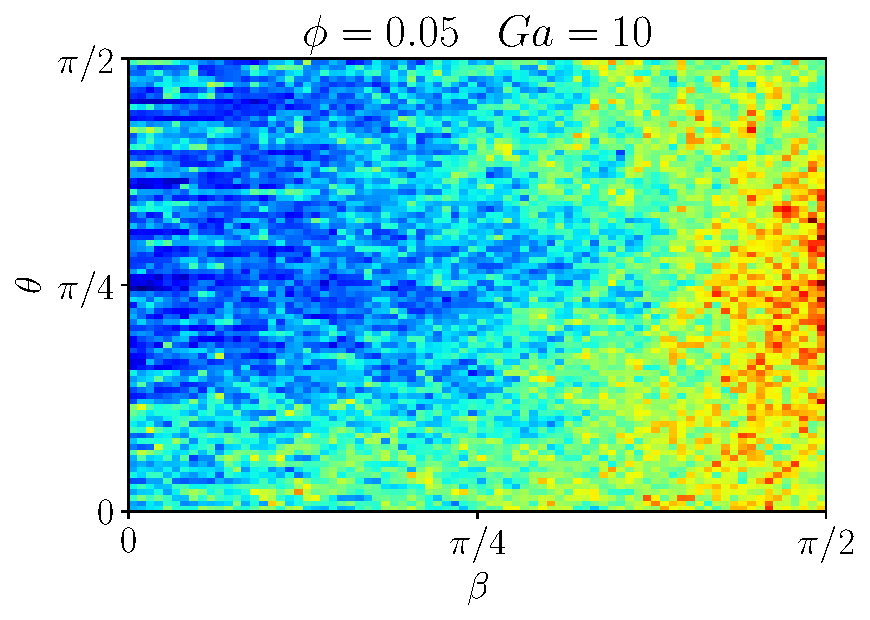
\includegraphics[height =\size]{image/N_10/beta/2DMAP_beta_theta_dmin_10_Bo0_5PHI0_05mu_r0_042Ga10.pdf}
    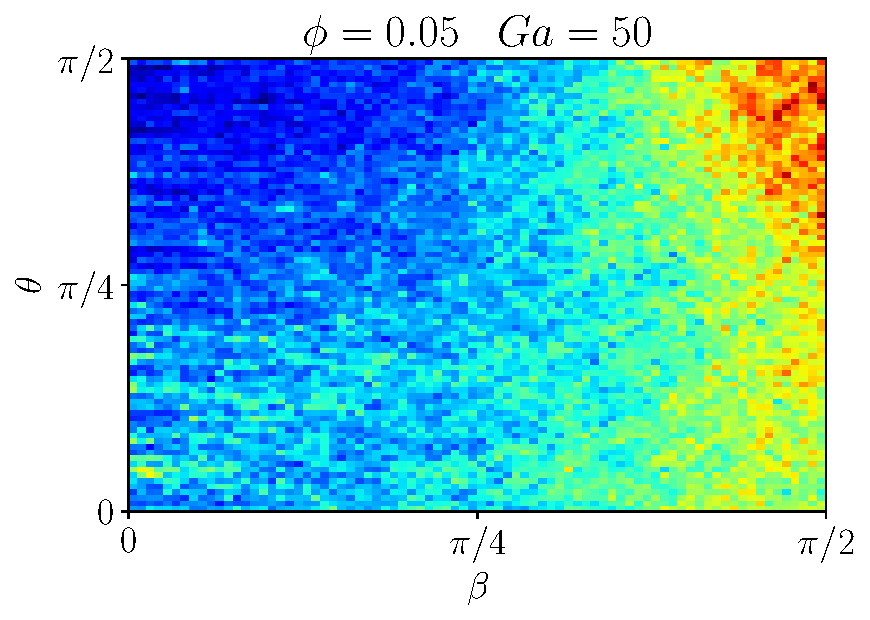
\includegraphics[height =\size]{image/N_10/beta/2DMAP_beta_theta_dmin_10_Bo0_5PHI0_05mu_r0_042Ga50.pdf}
    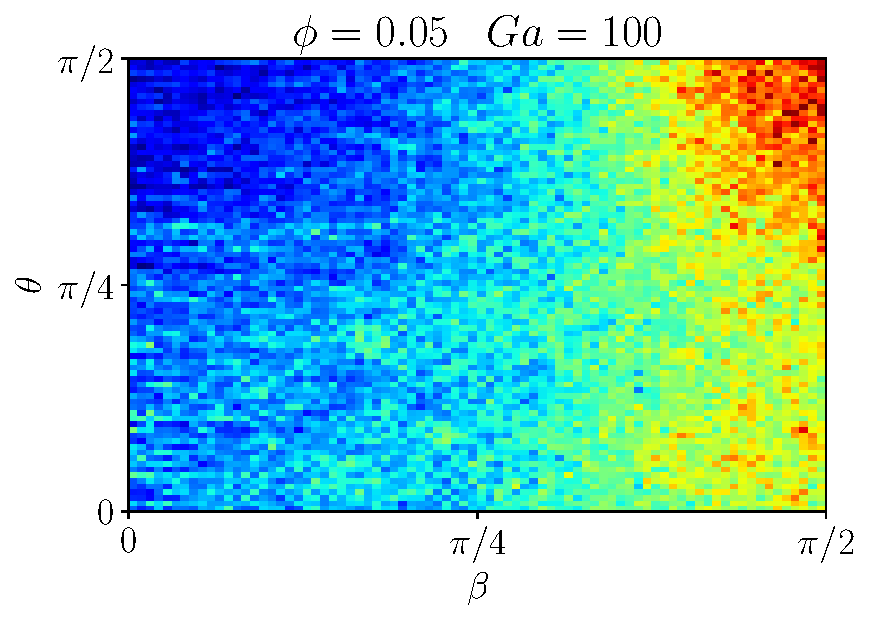
\includegraphics[height =\size]{image/N_10/beta/2DMAP_beta_theta_dmin_10_Bo0_5PHI0_05mu_r0_042Ga100.pdf}
    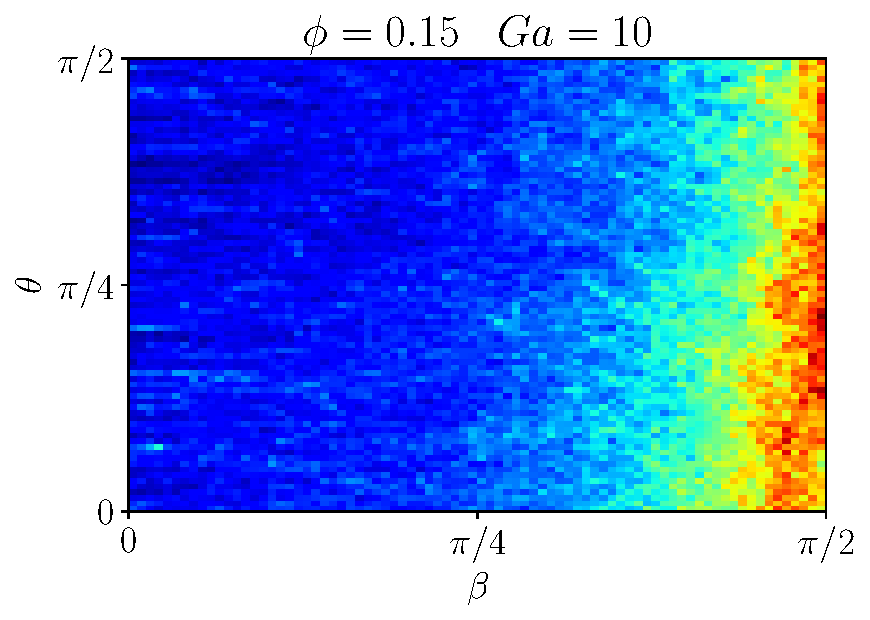
\includegraphics[height =\size]{image/N_10/beta/2DMAP_beta_theta_dmin_10_Bo0_5PHI0_15mu_r0_042Ga10.pdf}
    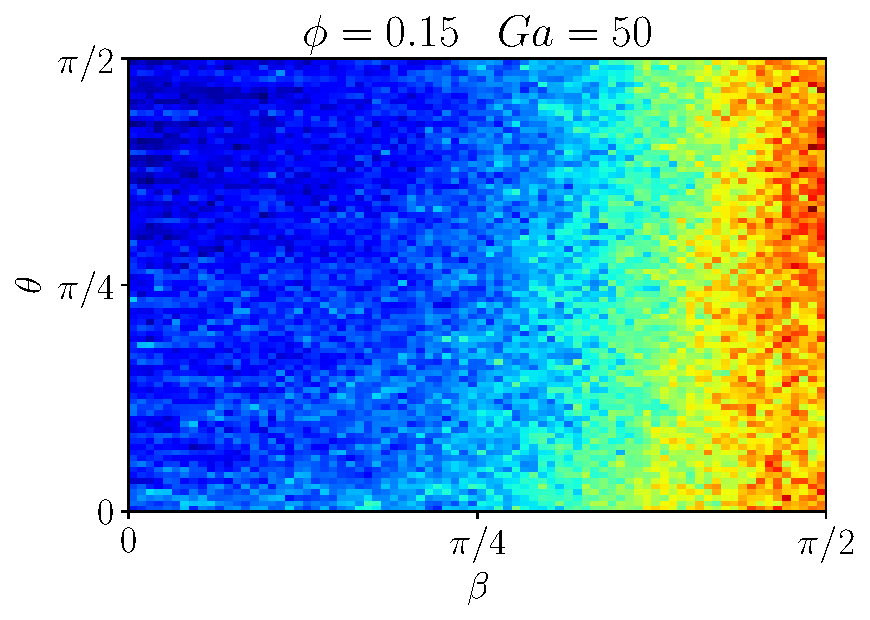
\includegraphics[height =\size]{image/N_10/beta/2DMAP_beta_theta_dmin_10_Bo0_5PHI0_15mu_r0_042Ga50.pdf}
    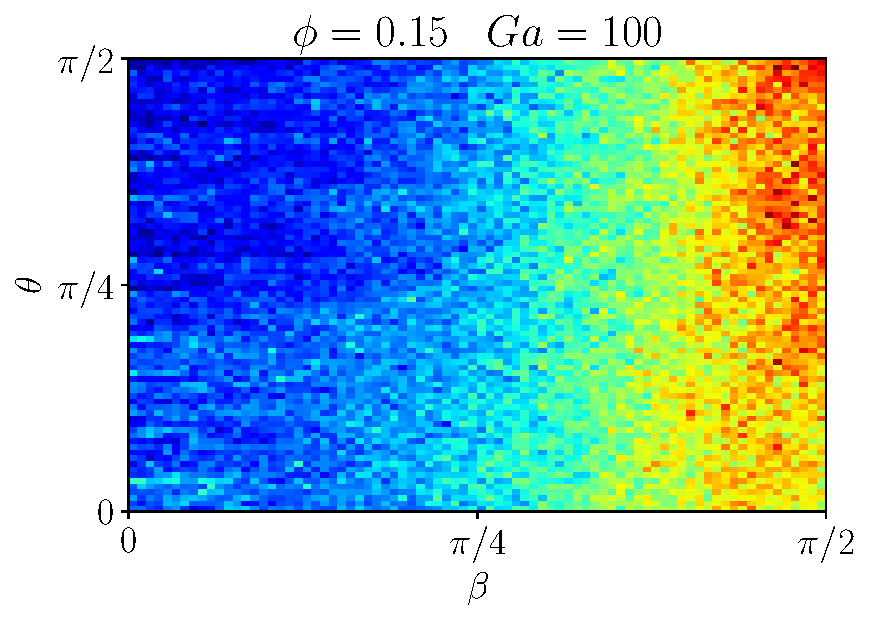
\includegraphics[height =\size]{image/N_10/beta/2DMAP_beta_theta_dmin_10_Bo0_5PHI0_15mu_r0_042Ga100.pdf}
    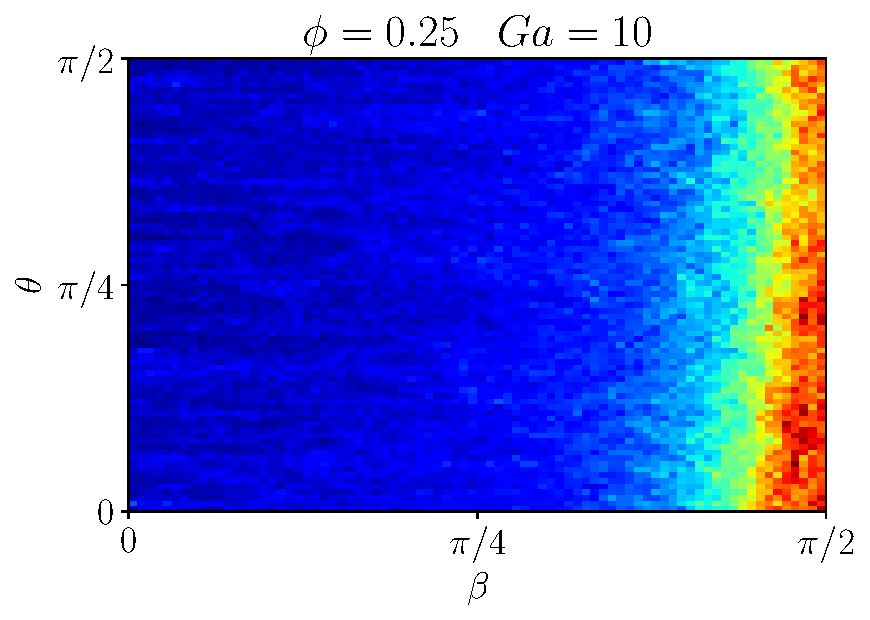
\includegraphics[height =\size]{image/N_10/beta/2DMAP_beta_theta_dmin_10_Bo0_5PHI0_25mu_r0_042Ga10.pdf}
    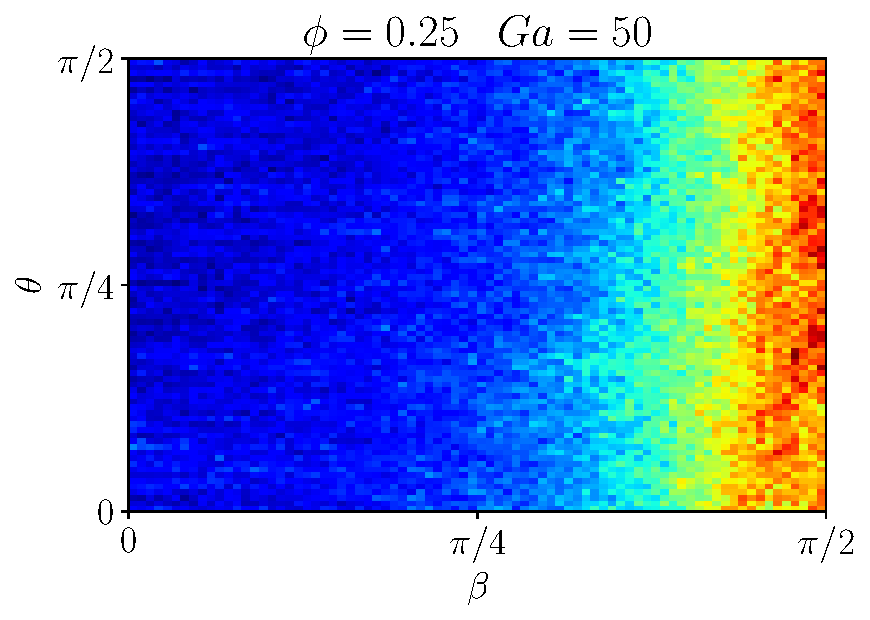
\includegraphics[height =\size]{image/N_10/beta/2DMAP_beta_theta_dmin_10_Bo0_5PHI0_25mu_r0_042Ga50.pdf}
    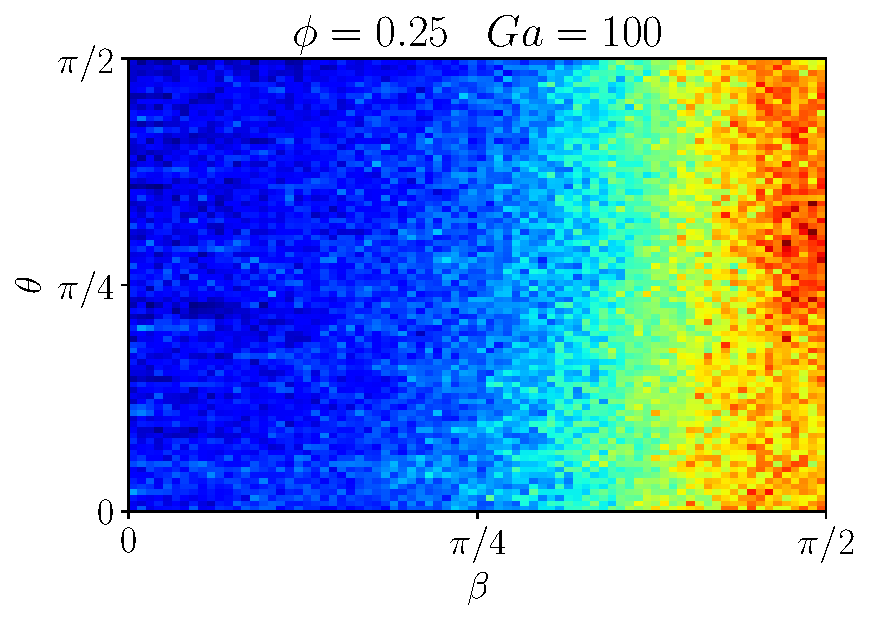
\includegraphics[height =\size]{image/N_10/beta/2DMAP_beta_theta_dmin_10_Bo0_5PHI0_25mu_r0_042Ga100.pdf}
    \caption{2 plots of $P_{\beta\theta}(\beta,\theta)$ for different $\phi$ and $Ga$ at $Bo = 0.5$ and $\mu_r = 0.042$. The color represents the density, it goes from blue meaning $P_{\beta\theta}(\beta,\theta)= P_{min}$, to red meaning $P_{\beta\theta}(\beta,\theta) = P_{max}$. The different plots are label from left to right and from top to bottom with the letters (a) to (i).} 
\end{figure} 
\begin{figure}[h!]
    \centering
    \includegraphics[height =\size]{image/N_10/beta/2DMAP_beta_theta_dmin_10_Bo0_5PHI0_05mu_r0_42Ga10.pdf}
    \includegraphics[height =\size]{image/N_10/beta/2DMAP_beta_theta_dmin_10_Bo0_5PHI0_05mu_r0_42Ga50.pdf}
    \includegraphics[height =\size]{image/N_10/beta/2DMAP_beta_theta_dmin_10_Bo0_5PHI0_05mu_r0_42Ga100.pdf}
    \includegraphics[height =\size]{image/N_10/beta/2DMAP_beta_theta_dmin_10_Bo0_5PHI0_15mu_r0_42Ga10.pdf}
    \includegraphics[height =\size]{image/N_10/beta/2DMAP_beta_theta_dmin_10_Bo0_5PHI0_15mu_r0_42Ga50.pdf}
    \includegraphics[height =\size]{image/N_10/beta/2DMAP_beta_theta_dmin_10_Bo0_5PHI0_15mu_r0_42Ga100.pdf}
    \includegraphics[height =\size]{image/N_10/beta/2DMAP_beta_theta_dmin_10_Bo0_5PHI0_25mu_r0_42Ga10.pdf}
    \includegraphics[height =\size]{image/N_10/beta/2DMAP_beta_theta_dmin_10_Bo0_5PHI0_25mu_r0_42Ga50.pdf}
    \includegraphics[height =\size]{image/N_10/beta/2DMAP_beta_theta_dmin_10_Bo0_5PHI0_25mu_r0_42Ga100.pdf}
    \caption{2 plots of $P_{\beta\theta}(\beta,\theta)$ for different $\phi$ and $Ga$ at $Bo = 0.5$ and $\mu_r = 0.42$. The color represents the density, it goes from blue meaning $P_{\beta\theta}(\beta,\theta)= P_{min}$, to red meaning $P_{\beta\theta}(\beta,\theta) = P_{max}$. The different plots are label from left to right and from top to bottom with the letters (a) to (i).} 
\end{figure} 
\begin{figure}[h!]
    \centering
    \includegraphics[height =\size]{image/N_10/beta/2DMAP_theta_distmin_dmin_10_Bo1PHI0_05mu_r0_42Ga10.pdf}
    \includegraphics[height =\size]{image/N_10/beta/2DMAP_theta_distmin_dmin_10_Bo1PHI0_05mu_r0_42Ga50.pdf}
    \includegraphics[height =\size]{image/N_10/beta/2DMAP_theta_distmin_dmin_10_Bo1PHI0_05mu_r0_42Ga100.pdf}
    \includegraphics[height =\size]{image/N_10/beta/2DMAP_theta_distmin_dmin_10_Bo1PHI0_15mu_r0_42Ga10.pdf}
    \includegraphics[height =\size]{image/N_10/beta/2DMAP_theta_distmin_dmin_10_Bo1PHI0_15mu_r0_42Ga50.pdf}
    \includegraphics[height =\size]{image/N_10/beta/2DMAP_theta_distmin_dmin_10_Bo1PHI0_15mu_r0_42Ga100.pdf}
    \includegraphics[height =\size]{image/N_10/beta/2DMAP_theta_distmin_dmin_10_Bo1PHI0_25mu_r0_42Ga10.pdf}
    \includegraphics[height =\size]{image/N_10/beta/2DMAP_theta_distmin_dmin_10_Bo1PHI0_25mu_r0_42Ga50.pdf}
    \includegraphics[height =\size]{image/N_10/beta/2DMAP_theta_distmin_dmin_10_Bo1PHI0_25mu_r0_42Ga100.pdf}
    \includegraphics[height =\size]{image/N_10/beta/2DMAP_theta_distmin_dmin_10_Bo1PHI0_05mu_r0_042Ga10.pdf}
    \includegraphics[height =\size]{image/N_10/beta/2DMAP_theta_distmin_dmin_10_Bo1PHI0_05mu_r0_042Ga50.pdf}
    \includegraphics[height =\size]{image/N_10/beta/2DMAP_theta_distmin_dmin_10_Bo1PHI0_05mu_r0_042Ga100.pdf}
    \caption{2 plots of $P_{d_{nbr}\theta}(d_{nbr},\theta)$ for different $\phi$ and $Ga$ at $Bo = 1$ and $\mu_r = 0.42$. The color represents the density, it goes from blue meaning $P_{d_{nbr}\theta}(d_{nbr},\theta)= P_{min}$, to red meaning $P_{d_{nbr}\theta}(d_{nbr},\theta) = P_{max}$. The different plots are label from left to right and from top to bottom with the letters (a) to (i).} 
\end{figure} 

\begin{figure}[h!]
    \centering
    \includegraphics[scale = 0.9,height = \size]{image/N_10/beta/2DMAP_beta_v_rel_dmin_10_Bo1PHI0_05mu_r0_42Ga10.pdf}
    \includegraphics[scale = 0.9,height = \size]{image/N_10/beta/2DMAP_beta_v_rel_dmin_10_Bo1PHI0_05mu_r0_42Ga50.pdf}
    \includegraphics[scale = 0.9,height = \size]{image/N_10/beta/2DMAP_beta_v_rel_dmin_10_Bo1PHI0_05mu_r0_42Ga100.pdf}
    \includegraphics[scale = 0.9,height = \size]{image/N_10/beta/2DMAP_beta_v_rel_dmin_10_Bo1PHI0_15mu_r0_42Ga10.pdf}
    \includegraphics[scale = 0.9,height = \size]{image/N_10/beta/2DMAP_beta_v_rel_dmin_10_Bo1PHI0_15mu_r0_42Ga50.pdf}
    \includegraphics[scale = 0.9,height = \size]{image/N_10/beta/2DMAP_beta_v_rel_dmin_10_Bo1PHI0_15mu_r0_42Ga100.pdf}
    \includegraphics[scale = 0.9,height = \size]{image/N_10/beta/2DMAP_beta_v_rel_dmin_10_Bo1PHI0_25mu_r0_42Ga10.pdf}
    \includegraphics[scale = 0.9,height = \size]{image/N_10/beta/2DMAP_beta_v_rel_dmin_10_Bo1PHI0_25mu_r0_42Ga50.pdf}
    \includegraphics[scale = 0.9,height = \size]{image/N_10/beta/2DMAP_beta_v_rel_dmin_10_Bo1PHI0_25mu_r0_42Ga100.pdf}
    \caption{2 plots of $P_{\beta\theta}(\beta,\theta)$ for different $\phi$ and $Ga$ at $Bo = 0.5$ and $\mu_r = 0.042$. The color represents the density, it goes from blue meaning $P_{\beta\theta}(\beta,\theta)= P_{min}$, to red meaning $P_{\beta\theta}(\beta,\theta) = P_{max}$. The different plots are label from left to right and from top to bottom with the letters (a) to (i).} 
    \label{fig:beta_u_rel_2D}
\end{figure} 

\begin{figure}[h!]
    \centering
    \includegraphics[height = \size]{image/N_10/beta/2DMAP_distmin_v_rel_dmax_10_Bo1PHI0_05mu_r0_42Ga10.pdf}
    \includegraphics[height = \size]{image/N_10/beta/2DMAP_distmin_v_rel_dmax_10_Bo1PHI0_05mu_r0_42Ga50.pdf}
    \includegraphics[height = \size]{image/N_10/beta/2DMAP_distmin_v_rel_dmax_10_Bo1PHI0_05mu_r0_42Ga100.pdf}
    \includegraphics[height = \size]{image/N_10/beta/2DMAP_distmin_v_rel_dmax_10_Bo1PHI0_15mu_r0_42Ga10.pdf}
    \includegraphics[height = \size]{image/N_10/beta/2DMAP_distmin_v_rel_dmax_10_Bo1PHI0_15mu_r0_42Ga50.pdf}
    \includegraphics[height = \size]{image/N_10/beta/2DMAP_distmin_v_rel_dmax_10_Bo1PHI0_15mu_r0_42Ga100.pdf}
    \includegraphics[height = \size]{image/N_10/beta/2DMAP_distmin_v_rel_dmax_10_Bo1PHI0_25mu_r0_42Ga10.pdf}
    \includegraphics[height = \size]{image/N_10/beta/2DMAP_distmin_v_rel_dmax_10_Bo1PHI0_25mu_r0_42Ga50.pdf}
    \includegraphics[height = \size]{image/N_10/beta/2DMAP_distmin_v_rel_dmax_10_Bo1PHI0_25mu_r0_42Ga100.pdf}
    \caption{2 plots of $P_{\beta\theta}(\beta,\theta)$ for different $\phi$ and $Ga$ at $Bo = 0.5$ and $\mu_r = 0.042$. The color represents the density, it goes from blue meaning $P_{\beta\theta}(\beta,\theta)= P_{min}$, to red meaning $P_{\beta\theta}(\beta,\theta) = P_{max}$. The different plots are label from left to right and from top to bottom with the letters (a) to (i).} 
    \label{fig:beta_u_rel_2D}
\end{figure} 

\subsection*{Distribution of $P_{\theta}$ and $P_{\beta}$}
\label{sec:dist_theta}
\begin{figure}[h!]
    \centering
    \includegraphics[height =\size]{image/N_10/beta/2DMAP_theta_dmin_10_Bo1PHI0_05mu_r0_042Ga10.pdf}
    \includegraphics[height =\size]{image/N_10/beta/2DMAP_theta_dmin_10_Bo1PHI0_05mu_r0_042Ga50.pdf}
    \includegraphics[height =\size]{image/N_10/beta/2DMAP_theta_dmin_10_Bo1PHI0_05mu_r0_042Ga100.pdf}
    \includegraphics[height =\size]{image/N_10/beta/2DMAP_theta_dmin_10_Bo1PHI0_15mu_r0_042Ga10.pdf}
    \includegraphics[height =\size]{image/N_10/beta/2DMAP_theta_dmin_10_Bo1PHI0_15mu_r0_042Ga50.pdf}
    \includegraphics[height =\size]{image/N_10/beta/2DMAP_theta_dmin_10_Bo1PHI0_15mu_r0_042Ga100.pdf}
    \includegraphics[height =\size]{image/N_10/beta/2DMAP_theta_dmin_10_Bo1PHI0_25mu_r0_042Ga10.pdf}
    \includegraphics[height =\size]{image/N_10/beta/2DMAP_theta_dmin_10_Bo1PHI0_25mu_r0_042Ga50.pdf}
    \includegraphics[height =\size]{image/N_10/beta/2DMAP_theta_dmin_10_Bo1PHI0_25mu_r0_042Ga100.pdf}
    \caption{2 plots of $P_{\theta}(\theta)$ for different $\phi$ and $Ga$ at $Bo = 0.5$ and $\mu_r = 0.042$. The color represents the density, it goes from blue meaning $P_{\theta}(\theta)= P_{min}$, to red meaning $P_{\theta}(\theta) = P_{max}$. The different plots are label from left to right and from top to bottom with the letters (a) to (i).} 
\end{figure} 
\begin{figure}[h!]
    \centering
    \includegraphics[height =\size]{image/N_10/beta/2DMAP_beta_dmin_10_Bo1PHI0_05mu_r0_042Ga10.pdf}
    \includegraphics[height =\size]{image/N_10/beta/2DMAP_beta_dmin_10_Bo1PHI0_05mu_r0_042Ga50.pdf}
    \includegraphics[height =\size]{image/N_10/beta/2DMAP_beta_dmin_10_Bo1PHI0_05mu_r0_042Ga100.pdf}
    \includegraphics[height =\size]{image/N_10/beta/2DMAP_beta_dmin_10_Bo1PHI0_15mu_r0_042Ga10.pdf}
    \includegraphics[height =\size]{image/N_10/beta/2DMAP_beta_dmin_10_Bo1PHI0_15mu_r0_042Ga50.pdf}
    \includegraphics[height =\size]{image/N_10/beta/2DMAP_beta_dmin_10_Bo1PHI0_15mu_r0_042Ga100.pdf}
    \includegraphics[height =\size]{image/N_10/beta/2DMAP_beta_dmin_10_Bo1PHI0_25mu_r0_042Ga10.pdf}
    \includegraphics[height =\size]{image/N_10/beta/2DMAP_beta_dmin_10_Bo1PHI0_25mu_r0_042Ga50.pdf}
    \includegraphics[height =\size]{image/N_10/beta/2DMAP_beta_dmin_10_Bo1PHI0_25mu_r0_042Ga100.pdf}
    \caption{2 plots of $P_{\beta}(\beta)$ for different $\phi$ and $Ga$ at $Bo = 0.5$ and $\mu_r = 0.042$. The color represents the density, it goes from blue meaning $P_{\beta}(\beta)= P_{min}$, to red meaning $P_{\beta}(\beta) = P_{max}$. The different plots are label from left to right and from top to bottom with the letters (a) to (i).} 
\end{figure} 
\begin{figure}[h!]
    \centering
    \includegraphics[height =\size]{image/N_10/beta/2DMAP_beta_dmin_10_Bo0_5PHI0_15mu_r0_042Ga10.pdf}
    \includegraphics[height =\size]{image/N_10/beta/2DMAP_beta_dmin_10_Bo1PHI0_15mu_r0_042Ga10.pdf}

    \includegraphics[height =\size]{image/N_10/beta/2DMAP_beta_dmin_10_Bo0_5PHI0_15mu_r0_42Ga10.pdf}
    \includegraphics[height =\size]{image/N_10/beta/2DMAP_beta_dmin_10_Bo1PHI0_15mu_r0_42Ga10.pdf}
    \caption{2 plots of $P_{\beta}(\beta)$ for different $\phi$ and $Ga$ at $Bo = 0.5$ and $\mu_r = 0.042$. The color represents the density, it goes from blue meaning $P_{\beta}(\beta)= P_{min}$, to red meaning $P_{\beta}(\beta) = P_{max}$. The different plots are label from left to right and from top to bottom with the letters (a) to (i).} 
    \label{fig:beta_bomu}
\end{figure} 
\end{document}
